\documentclass[12pt, openany, oneside]{book}

\usepackage{listings}
\usepackage[dvipsnames]{xcolor}
\usepackage{ctex}
\usepackage{fontspec}
\usepackage{setspace}
\usepackage{tikz}
\usepackage{anyfontsize}
\usepackage{sectsty}
\usepackage{titlesec}
\usepackage{float}
\usepackage[hidelinks]{hyperref}
\usepackage[a4paper]{geometry}
\usepackage{url}
\usepackage{amssymb}
\usepackage{fontawesome5}
\usepackage[most]{tcolorbox}
\usepackage{stackengine}
\usepackage{multirow}
\usepackage{makecell}
\usepackage[T1]{fontenc}
\usepackage{diagbox}
\usepackage{longtable}
\usepackage{newtxtt}
\usepackage{pgf-umlcd}
\usepackage{bbding}
\usepackage[edges]{forest}
\usepackage{amsmath}
\usepackage{algorithm}
\usepackage{algpseudocode}
\usepackage{tkz-graph}
\usepackage{drawstack}
\usepackage{dcolumn}

\usetikzlibrary{calc,trees,positioning,arrows,fit,shapes}
\usetikzlibrary{shapes.multipart,chains}
\usetikzlibrary{shadows}
\usetikzlibrary{arrows.meta}
\usetikzlibrary{matrix,backgrounds}

\tikzset{iv/.style={draw,fill=red!50,circle,minimum size=20pt,inner
sep=0pt,text=black},ev/.style={draw,fill=yellow,rectangle,minimum
size=20pt,inner sep=0pt,text=black}}

\tikzstyle{redVertex}  =[draw,fill=red,     circle,minimum size=18pt,inner sep=0pt, text=white]
\tikzstyle{blackVertex}=[draw,fill=black,   circle,minimum size=18pt,inner sep=0pt, text=white]
\tikzstyle{nil}        =[draw,fill=black,rectangle,minimum size=18pt,inner sep=0pt, text=white]

\tikzset{block/.style={
        font=\sffamily,
        draw=black,
        thin,
        fill=pink!50,
        rectangle split,
        rectangle split horizontal,
        rectangle split parts=#1,
        outer sep=0pt},
        gblock/.style={
            block,
            rectangle split parts=#1,
            fill=green!30}
        }

\tikzstyle{ptr}  = [draw, -{Stealth[scale=1.0]}, blue]
\tikzstyle{head} = [rectangle, draw, text height=3mm, text width=3mm,
                    text centered, node distance=3cm, inner sep=0pt]
\tikzstyle{data} = [rectangle split, rectangle split parts=2, draw,
                    text centered, minimum height=3em]
\newcommand{\data}{
  data \nodepart{second}
  \phantom{\texttt{NULL}}
}

\tikzset{
    queue element/.style={
        draw,very thin,rounded corners,
        fill=yellow!30,
        minimum width=1cm,minimum height=.5cm,
        font=\sffamily\footnotesize
    },
    >={[scale=0.8]Triangle},
    queue/.style={matrix of nodes,
        nodes in empty cells,
        nodes={queue element, anchor=center},
        fill=green!20,
        column sep=5mm,
        row sep=2mm,
    },
}

\def\x{0}
\def\y{0}
\def\k{0}
\def\radius{5}

\makeatletter
\newcommand{\verbatimfont}[1]{\renewcommand{\verbatim@font}{\ttfamily#1}}
\makeatother

\makeatletter
\def\BState{\State\hskip-\ALG@thistlm}
\makeatother

\tikzstyle{startend} = [rectangle, rounded corners, minimum width=3cm, minimum height=1cm, text centered, draw=black, fill=red!30]
\tikzstyle{io}        = [trapezium, trapezium left angle=70, trapezium right angle=110, minimum width=3cm, inner xsep = -15pt, minimum height=1cm, text centered, draw=black, fill=blue!30]
\tikzstyle{process}   = [rectangle, minimum width=3cm, minimum height=1cm, inner ysep=0, text centered, draw=black, fill=orange!30]
\tikzstyle{decision}  = [diamond,shape aspect=2.5, minimum width=3cm, minimum height=1cm, inner xsep=0,text centered, draw=black, fill=green!30]
\tikzstyle{arrow}     = [thick,->,>=stealth]

\def\rlwd{.5pt} \def\rlht{2.2ex} \def\rldp{.5ex}
\def\mydiv#1{~
  \rule[-\rldp]{\rlwd}{\rlht}
  \setbox0=\hbox{~#1}
  \stackunder[\dimexpr\rldp-\rlwd]{~#1}{\rule{\wd0}{\rlwd}}%
}

\definecolor{mycolor}{RGB}{0,128,128}
\newtcbox{\mybox} {
    on line,
    colback=mycolor,
    fontupper=\bfseries\color{white},
    boxrule=0pt,
    arc=5pt, 
    boxsep=0pt, 
    left=2pt, 
    right=2pt, 
    top=5pt, 
    bottom=5pt
}

\setstretch{1.5}
\setlength{\parindent}{0cm}

\geometry{a4paper,top=2.5cm,bottom=2.5cm}

\titleformat{\chapter}{\Huge\Huge\bfseries}{\chaptertitlename\ \thechapter{\ }}{0pt}{\Huge}{}
\titlespacing{\chapter}{0pt}{0pt}{12pt}

\definecolor{dkgreen}{rgb}{0,0.4,0}
\definecolor{gray}{rgb}{0.5,0.5,0.5}
\definecolor{mauve}{rgb}{0.58,0,0.82}
\definecolor{LightGray}{gray}{0.9}

\lstset{
    basicstyle=\linespread{1.3} \fontspec{Consolas},    %  the size of the fonts that are used for the code
	basewidth=0.5em,
    numbers=left,            % where to put the line-numbers
    numberstyle=\color{black},  % the style that is used for the line-numbers
    numbersep=10pt,                  % how far the line-numbers are from the code
    backgroundcolor=\color{white},
    showspaces=false,
    showstringspaces=false,
    showtabs=false,
    frame=single,                   % adds a frame around the code
    rulecolor=\color{black},        % if not set, the frame-color may be changed on line-breaks within not-black text (e.g. commens (green here))
    tabsize=4,                      % sets default tabsize to 2 spaces
    captionpos=t,                   % sets the caption-position to bottom
    breaklines=false,                % sets automatic line breaking
    breakatwhitespace=true,        % sets if automatic breaks should only happen at whitespace
    title=\lstname,                   % show the filename of files included with \lstinputlisting;
    % also try caption instead of title
    numberstyle=\color{black},		% line number color
    keywordstyle=\color{blue},          % keyword style
    commentstyle=\color{dkgreen},       % comment style
    stringstyle=\color{mauve},         % string literal style
    escapeinside={\%*}{*)},            % if you want to add LaTeX within your code
    morekeywords={*,...}               % if you want to add more keywords to the set
}

\begin{document}

\thispagestyle{empty}

\begin{tikzpicture}[overlay,remember picture]
	\fill[
		black!2]
	(current page.south west) rectangle (current page.north east);

	\shade[
		left color=Dandelion,
		right color=Dandelion!40,
		transform canvas ={rotate around ={45:($(current page.north west)+(0,-6)$)}}]
	($(current page.north west)+(0,-6)$) rectangle ++(9,1.5);

	\shade[
		left color=lightgray,
		right color=lightgray!50,
		rounded corners=0.75cm,
		transform canvas ={rotate around ={45:($(current page.north west)+(.5,-10)$)}}]
	($(current page.north west)+(0.5,-10)$) rectangle ++(15,1.5);

	\shade[
		left color=lightgray,
		rounded corners=0.3cm,
		transform canvas ={rotate around ={45:($(current page.north west)+(.5,-10)$)}}] ($(current page.north west)+(1.5,-9.55)$) rectangle ++(7,.6);

	\shade[
		left color=orange!80,
		right color=orange!60,
		rounded corners=0.4cm,
		transform canvas ={rotate around ={45:($(current page.north)+(-1.5,-3)$)}}]
	($(current page.north)+(-1.5,-3)$) rectangle ++(9,0.8);

	\shade[
		left color=red!80,
		right color=red!80,
		rounded corners=0.9cm,
		transform canvas ={rotate around ={45:($(current page.north)+(-3,-8)$)}}] ($(current page.north)+(-3,-8)$) rectangle ++(15,1.8);

	\shade[
		left color=orange,
		right color=Dandelion,
		rounded corners=0.9cm,
		transform canvas ={rotate around ={45:($(current page.north west)+(4,-15.5)$)}}]
	($(current page.north west)+(4,-15.5)$) rectangle ++(30,1.8);

	\shade[
		left color=RoyalBlue,
		right color=Emerald,
		rounded corners=0.75cm,
		transform canvas ={rotate around ={45:($(current page.north west)+(13,-10)$)}}]
	($(current page.north west)+(13,-10)$) rectangle ++(15,1.5);

	\shade[
		left color=lightgray,
		rounded corners=0.3cm,
		transform canvas ={rotate around ={45:($(current page.north west)+(18,-8)$)}}]
	($(current page.north west)+(18,-8)$) rectangle ++(15,0.6);

	\shade[
		left color=lightgray,
		rounded corners=0.4cm,
		transform canvas ={rotate around ={45:($(current page.north west)+(19,-5.65)$)}}]
	($(current page.north west)+(19,-5.65)$) rectangle ++(15,0.8);

	\shade[
		left color=OrangeRed,
		right color=red!80,
		rounded corners=0.6cm,
		transform canvas ={rotate around ={45:($(current page.north west)+(20,-9)$)}}]
	($(current page.north west)+(20,-9)$) rectangle ++(14,1.2);

	% Title
	\node[align=center] at ($(current page.center)+(0,-7)$)
	{
	{\fontsize{60}{60} \selectfont {{数据结构与算法}}}\\[1cm]
	{\fontsize{40}{40} \selectfont {{Data Structure and Algorithm}}}\\[2cm]
	{\fontsize{20}{19.2} \selectfont \textcolor{orange}{ \bf 极夜酱}}\\[4pt]
	};
\end{tikzpicture}

\newpage

\pagestyle{plain}
\setcounter{page}{1}
\setcounter{tocdepth}{1}
\tableofcontents

\newpage

\setcounter{page}{1}

% \part{基础篇}

% \chapter{数据结构与算法}

\section{算法}

\subsection{算法(Algorithm)}

算法是一个很古老的概念,最早来自数学领域。 \\

有一个关于算法的小故事:在很久很久以前,曾经有一个顽皮又聪明的熊孩子,天天在课堂上调皮捣蛋。终于有一天,老师忍无可忍,对熊孩子说:“臭小子,你又调皮啊!今天罚你做加法,算出$ 1 + 2 + 3 + \dots + 9999 + 10000 $累加的结果,算不完不许回家!”  \\

老师以为,熊孩子会按部就班地一步一步计算:

\vspace{-1cm}

\begin{align*}
	1 + 2  & = 3  \\
	3 + 3  & = 6  \\
	6 + 4  & = 10 \\
	10 + 5 & = 15 \\
	\dots
\end{align*}

这还不得算到明天天亮?够这小子受的!老师心里幸灾乐祸地想着。谁知仅仅几分钟后…… \\

“老师,我算完了!结果是50005000,对不对?” \\

“这,这,这……你小子怎么算得这么快?我读书多,你骗不了我的!” \\

看着老师惊讶的表情,熊孩子微微一笑,讲出了他的计算方法。 \\

首先把从1到10000这10000个数字两两分组相加:

\vspace{-1cm}

\begin{align*}
	1 + 10000 & = 10001 \\
	2 + 9999  & = 10001 \\
	3 + 9998  & = 10001 \\
	4 + 9997  & = 10001 \\
	\dots
\end{align*}

一共有$ 10000 \div 2 = 5000 $组,所以1到10000相加的总和可以这样来计算:

$$
	(1 + 10000) \times 10000 \div 2 = 50005000
$$

这个熊孩子就是后来著名的犹太数学家约翰·卡尔·弗里德里希·高斯,而他所采用的这种等差数列求和的方法,被称为高斯算法。 \\

算法是解决问题的一种方法或一个过程,是一个由若干运算或指令组成的有穷序列。求解问题的算法可以看作是输入实例与输出之间的函数。 \\

算法有5个特点:

\begin{enumerate}
	\item 有穷性(finiteness):算法必须能在执行有限个步骤之后终止。
	\item 确定性(definiteness):算法的每一步骤必须有确切的定义。
	\item 输入项(input):一个算法有0个或多个输入。
	\item 输出项(output):一个算法有一个或多个输出,没有输出的算法是毫无意义的。
	\item 可行性(effectiveness):算法中执行的任何计算步骤都是可以被分解为基本的可执行的操作步。
\end{enumerate}

\subsection{算法描述}

算法是可完成特定任务的一系列步骤,算法的计算过程定义明确,通过一些值作为输入并产生一些值作为输出。 \\

流程图(flow chart)是算法的一种图形化表示方式,使用一组预定义的符号来说明如何执行特定任务。

\begin{itemize}
	\item 圆角矩形:开始和结束
	\item 矩形:数据处理
	\item 平行四边形:输入/输出
	\item 菱形:分支判断条件
	\item 流程线:步骤
\end{itemize}

\begin{figure}[H]
	\centering
	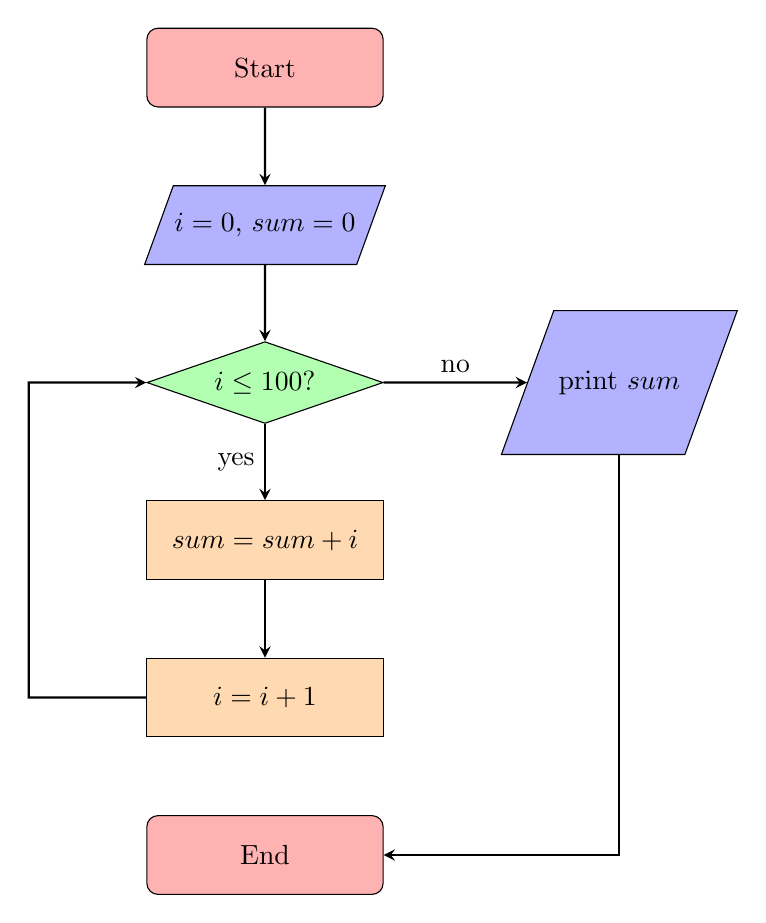
\begin{tikzpicture}[node distance=2cm]
		\node (start) [startend] {Start};
		\node (init)   [io, below of=start] {$ i = 0 $, $ sum = 0 $};
		\node (decision)  [decision, below of=init] {$ i \le 100 $?};
		\node (accumulation) [process, below of=decision] {$ sum = sum + i $};
		\node (update) [process, below of=accumulation] {$ i = i + 1 $};
		\node (output) [io, right of=decision, xshift=2.5cm] {print $ sum $};
		\node (end) [startend, below of=update] {End};

		\draw [arrow] (start) -- (init);
		\draw [arrow] (init) -- (decision);
		\draw [arrow] (decision) -- node[anchor=east] {yes } (accumulation);
		\draw [arrow] (accumulation) -- (update);
		\draw [arrow] (update) -- (-3,-8) -- (-3,-4) -- (decision);
		\draw [arrow] (decision) -- node[anchor=south] {no} (output);
		\draw [arrow] (output) |- (end);
	\end{tikzpicture}
	\caption{计算$ \sum_{i=1}^{100} i $的流程图}
\end{figure}

伪代码(pseudocode)是一种非正式的,类似于英语结构的,用于描述模块结构图的语言。使用伪代码的目的是使被描述的算法可以容易地以任何一种编程语言实现。

\begin{algorithm}[H]
	\caption{插入排序}
	\begin{algorithmic}[1]
		\Procedure{insertionSort}{A[0..n-1]}
		\For {j = 2 to n - 1}
		\State key = A[j]
		\State i = j - 1
		\While {i > 0 and A[i] > key}
		\State A[i+1] = A[i]
		\State i = i - 1
		\EndWhile
		\State A[i+1] = key
		\EndFor
		\State \Return A
		\EndProcedure
	\end{algorithmic}
\end{algorithm}

\newpage

\section{算法效率}

\subsection{算法效率}

算法有高效的,也有拙劣的。在高斯的故事中,高斯所用的算法显然是更加高效的算法,它利用等差数列的规律,四两拨千斤,省时省力地求出了最终结果。而老师心中所想的算法,按部就班地一个数一个数进行累加,则是一种低效、笨拙的算法。虽然这种算法也能得到最终结果,但是其计算过程要低效得多。 \\

在计算机领域,我们同样会遇到各种高效和拙劣的算法。衡量算法好坏的重要标准有两个:时间复杂度、空间复杂度。 \\

让我们来想象一个场景:某一天,小灰和大黄同时加入了同一家公司。老板让他们完成一个需求。一天后,小灰和大黄交付了各自的代码,两人的代码实现的功能差不多。但是,大黄的代码运行一次要花100 ms,占用内存5 MB;小灰的代码运行一次要花100 s,占用内存500 MB。 \\

“小灰,收拾东西走人,明天不用来上班了!” \\

小灰虽然也按照老板的要求实现了功能,但他的代码存在两个很严重的问题:运行时间长、占用空间大。 \\

算法效率分析指的是算法求解一个问题所需要的时间资源和空间资源。效率可以通过对算法执行基本运算(步数)的数目进行估算,度量一个算法运算时间的三种方式:

\begin{itemize}
	\item 最好情形时间复杂度
	\item 最坏情形时间复杂度
	\item 平均情形时间复杂度
\end{itemize}

最坏情形是任何规模为n的问题实例运行时间的上界,即任何规模为n的实例,其运行时间都不会超过最坏情况的运行时间。 \\

对某些算法,最坏情况经常发生。例如在某个数据库中查询不存在的某条诗句就是查询算法的最坏情形。平均情形有时跟最坏情形差不多。

\subsection{时间复杂度(Time Complexity)}

算法的效率主要取决于算法本身,与计算模型(例如计算机)无关,这样可以通过分析算法的运行时间从而比较出算法之间的快慢。分析一个算法的运行时间应该主要关注与问题规模有关的主要项,其它低阶项,甚至主要项的常数系数都可以忽略。 \\

渐进时间复杂度用大写$ O $来表示,所以也被称为大$ O $表示法。

时间复杂度有如下原则:

\begin{enumerate}
	\item 如果运行时间是常数量级,则用$ O(1) $表示。
	\item 只保留时间函数中的最高阶项。
	\item 如果最高阶项存在,则省去最高阶项前面的系数。
\end{enumerate}

在编程的世界中有各种各样的算法,有许多不同形式的时间复杂度,例如:$ O(1) $、$ O(logn) $、$ O(n) $、$ O(nlogn) $、$ O(n^2) $、$ O(2^n) $、$ O(n!) $等。

\subsection{空间复杂度(Space Complexity)}

内存空间是有限的,在时间复杂度相同的情况下,算法占用的内存空间自然是越小越好。如何描述一个算法占用的内存空间的大小呢?这就用到了算法的另一个重要指标——空间复杂度。 \\

和时间复杂度类似,空间复杂度是对一个算法在运行过程中临时占用存储空间大小的量度,它同样使用了大$ O $表示法。 \\

正所谓鱼和熊掌不可兼得,很多时候,我们不得不在时间复杂度和空间复杂度之间进行取舍。在绝大多数时候,时间复杂度更为重要一些,我们宁可多分配一些内存空间,也要提升程序的执行速度。

\newpage

\section{基础算法}

\subsection{暴力枚举}

暴力破解法也称穷举法,思想就是列举出所有可能情况,然后根据条件判断此答案是否合适,合适就保留,不合适就丢弃。暴力法主要利用计算机运算速度快、精确度高的特点。因此暴力法是通过牺牲时间来换取答案的全面性。 \\

\mybox{鸡兔同笼} \\

上有三十五头,下有九十四足,问鸡兔各几何?

\begin{lstlisting}[language=C]
void count(int head, int foot) {
	for(int chicken = 0; chicken <= head; chicken++) {
		int rabbit = head - chicken;
		if(chicken*2 + rabbit*4 == foot) {
			printf("鸡:%2d\t兔:%2d\n", chicken, rabbit);
		}
	}
}
\end{lstlisting}

\vspace{0.5cm}

\mybox{百钱买百鸡} \\

公鸡5文钱1只,母鸡3文钱1只,小鸡1文钱3只,如果用100文钱买100只鸡,那么公鸡、母鸡和小鸡各应该买多少只?

\begin{lstlisting}[language=C]
void buy(int n, int money) {
	for(int x = 0; x <= n/5; x++) {
		for(int y = 0; y <= n/3; y++) {
			int z = n - x - y;
			if(z > 0 && z % 3 == 0 && 5*x + 3*y + z/3 == money) {
				printf("公鸡:%3d\t母鸡:%3d\t小鸡:%3d\n", x, y, z);
			}
		}
	}
}
\end{lstlisting}

\subsection{字符串逆序}

将一个字符串中的字符顺序颠倒过来实现逆序。 \\

\mybox{字符串逆序}

\begin{lstlisting}[language=C]
void reverse(char *str) {
	int i = 0;
	int j = strlen(str) - 1;
	while(i < j) {
		char temp = str[i];
		str[i] = str[j];
		str[j] = temp;
		i++;
		j--;
	}
}
\end{lstlisting}

\subsection{随机算法}

随机算法就是在算法中引入随机因素,通过随机数选择算法的下一步操作,它采用了一定程序的随机性作为其逻辑的一部分。 \\

只有随机数生成器的情况下如何计算圆周率的近似值?蒙特卡洛算法就是一种随机算法,用于近似计算圆周率$ \pi $的值。 \\

蒙特卡洛算法是以概率和统计理论方法为基础的一种计算方法,将所求解的问题同一定的概率模型相联系,用电子计算机实现统计模拟或抽样,以获得问题的近似解。为象征性地表明这一方法的概率统计特征,故借用赌城蒙特卡罗命名。 \\

蒙特卡洛算法的基本思想就是当样本数量足够大时,可以用频率去估计概率,这也是求圆周率$ \pi $的常用方法。

\begin{figure}[H]
	\centering
	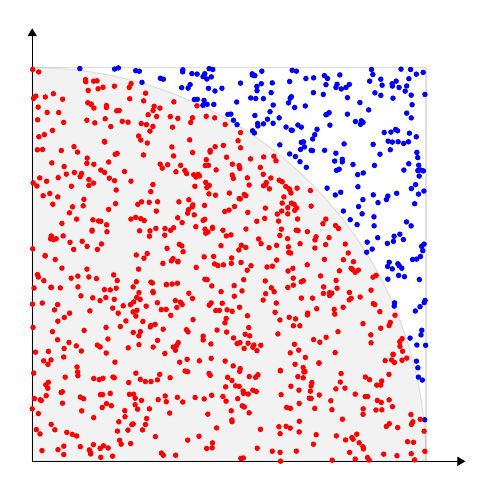
\begin{tikzpicture}
		\draw[fill=gray, opacity=0.1] (\radius,0) arc(0:90:\radius) -- (0,0) -- cycle;
		\draw[gray, opacity=0.25] (0,0) rectangle (\radius,\radius);
		\draw[->] (0,0) -- (1.1*\radius,0);
		\draw[->] (0,0) -- (0,1.1*\radius);
		\foreach \i in {1,2,...,1000}{
				\typeout{Point \i}
				\pgfmathsetmacro\x{\radius*rnd}
				\typeout{X \x}
				\pgfmathsetmacro\y{\radius*rnd}
				\typeout{Y \y}
				\pgfmathsetmacro\k{(pow(\x,2)+pow(\y,2)) <pow(\radius,2)}
				\typeout{im Kreis?: \k}
				\pgfmathparse{ifthenelse(\k==1,"red","blue")}
				\fill[\pgfmathresult] (\x,\y)circle(1pt);
			}
	\end{tikzpicture}
	\caption{蒙特卡洛算法}
\end{figure}


当在$ [0, 1] $的范围内随机选择一个坐标$ (x, y) $时,每个坐标点被选中的概率相等,则坐标落在直径为1的正方形中的圆的概率为:

$$
	P \left( \sqrt{x^2 + y^2} \le 1 \right) = {\pi \over 4}
$$

在生成大量随机点的前提下能得到尽可能接近圆周率的值。 \\

\mybox{蒙特卡罗算法}

\begin{lstlisting}[language=C]
double montePI(int n) {
	int cnt = 0;        // 圆内点的数量
	for(int i = 0; i < n; i++) {
		double x = rand() / (RAND_MAX + 1.0);   // [0, 1]
		double y = rand() / (RAND_MAX + 1.0);   // [0, 1]
		if(sqrt(x*x + y*y) <= 1) {
			cnt++;
		}
	}
	return 4.0 * cnt / n;
}
\end{lstlisting}

\newpage

\section{数据结构}

\subsection{数据结构(Data Structure)}

数据结构是算法基石,是计算机数据的组织、管理和存储的方式,数据结构指的是相互之间存在一种或多种特定关系的数据元素的集合。一个好的数据结构可以带来更高的运行或者存储效率。 \\

\begin{figure}[H]
	\centering
	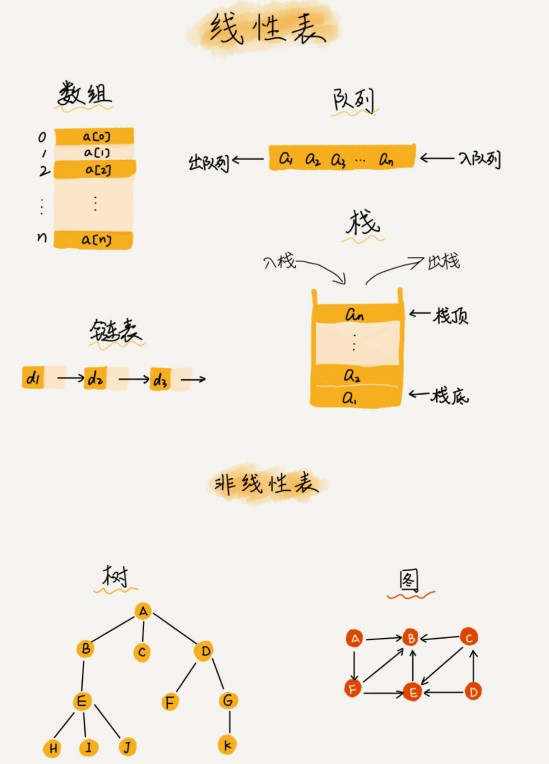
\includegraphics[]{img/C1/1-4/1.png}
	\caption{常用数据结构}
\end{figure}

\newpage
% \chapter{数组}

\section{数组}

\subsection{数组(Array)}

数组是数据结构中最简单的结构,很多编程语言都内置数组。数组是有限个相同类型的变量所组成的集合,数组中的每一个变量被称为元素。\\

创建数组时会在内存中划分出一块连续的内存,将数据按顺序进行存储,数组中的每一个元素都有着自己的下标(index),下标从0开始一直到数组长度-1。因为数组在存储数据时是按顺序存储的,存储数据的内存也是连续的。\\

对于数组来说,读取元素是最简单的操作。由于数组在内存中顺序存储,所以只要给出数组的下标,就可以读取到对应位置的元素。像这种根据下标读取元素的方式叫作随机读取。但是需要注意的是,数组的下标范围必须在0到数组长度-1之内,否则会出现数组越界。数组读取元素的时间复杂度是$ O(1) $。\\

数组拥有非常高效的随机访问能力,只要给出下标,就可以用常量时间找到对应元素。有一种高效查找元素的算法叫作二分查找,就是利用了数组的这个优势。\\

数组的劣势体现在插入和删除元素方面。由于数组元素连续紧密地存储在内存中,插入、删除元素都会导致大量元素被迫移动,影响效率。总的来说,数组所适合的是读操作多、写操作少的场景。\\

\mybox{更新数组元素}

\begin{lstlisting}[language=Python]
arr = [3, 1, 2, 5, 4, 9, 7, 2]
arr[5] = 10
print(arr[5])
\end{lstlisting}

\newpage

\section{查找算法}

\subsection{顺序查找(Sequence Search)}

顺序查找也称线性查找,是一种按照序列原有顺序进行遍历比较查询的基本查找算法。\\

对于任意一个序列以及一个需要查找的元素(关键字),将关键字与序列中元素依次比较,直到找出与给定关键字相同的元素,或者将序列中的元素与其都比较完为止。若某个元素的值与关键字相等,则查找成功;如果直到最后一个元素,元素的值和关键字比较都不等时,则查找不成功。\\

最好的情况就是在第一个位置就找到,算法时间复杂度为$ O(1) $。\\

最坏情况是关键字不存在,需要进行$ n $次比较,时间复杂度为$ O(n) $。\\

平均查找次数为$ (n + 1) / 2 $,平均时间复杂度为$ O(n) $。\\

\mybox{顺序查找}

\begin{lstlisting}[language=C]
int sequence_search(int *arr, int n, int key) {
    for (int i = 0; i < n; i++) {
        if (arr[i] == key) {
            return i;
        }
    }
    return -1;
}
\end{lstlisting}

\vspace{0.5cm}

\subsection{二分查找(Binary Search)}

二分查找法也称折半查找,是一种效率较高的查找方法。折半查找要求线性表必须采用顺序存储结构,而且表中元素按关键字有序排列。\\

算法思想是假设表中元素是按升序排列,将表中间位置的关键字与查找关键字比较,如果两者相等,则查找成功;否则利用中间位置记录将表分成前、后两个子表,如果中间位置的关键字大于查找关键字,则进一步查找前一子表,否则进一步查找后一子表。重复以上过程,直到找到满足条件的记录,使查找成功,或直到子表不存在为止,此时查找不成功。\\

二分查找法的时间复杂度为$ O(logn) $。\\

\mybox{二分查找}

\begin{lstlisting}[language=C]
int binary_search(int *arr, int n, int key) {
    int start = 0;
    int end = n - 1;
    while (start <= end) {
        int mid = (start + end) / 2;
        if (arr[mid] == key) {
            return mid;
        } else if (arr[mid] < key) {
            start = mid + 1;
        } else {
            end = mid - 1;
        }
    }
    return -1;
}
\end{lstlisting}

\newpage

\section{数组元素插入与删除}

\subsection{插入元素}

在数组中插入元素存在3种情况:

\begin{figure}[H]
	\centering
	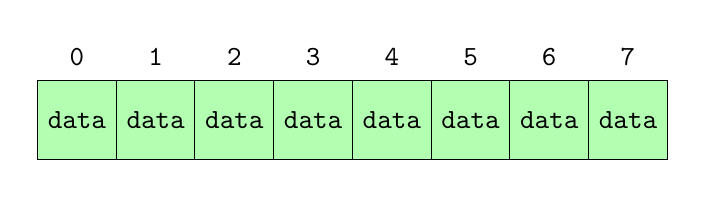
\begin{tikzpicture}[font=\ttfamily,
			array/.style={matrix of nodes,nodes={draw, minimum size=10mm, fill=green!30},column sep=-\pgflinewidth, row sep=0.5mm, nodes in empty cells,
					row 1/.style={nodes={draw=none, fill=none, minimum size=5mm}},
				}]

		\matrix[array] (array) {
			0    & 1    & 2    & 3    & 4    & 5    & 6    & 7    \\
			data & data & data & data & data & data & data & data \\
		};
	\end{tikzpicture}
	\caption{数组}
\end{figure}

\subsubsection{尾部插入}

直接把插入的元素放在数组尾部的空闲位置即可。

\subsubsection{中间插入}

首先把插入位置及后面的元素向后移动,腾出位置,再把要插入的元素放入该位置上。\\

\mybox{插入元素}

\begin{lstlisting}[language=C]
int insert(int *arr, int n, int index, int val) {
    if(index < 0 || index >= n) {
        return n;
    }
    for(int i = n - 1; i >= index; i--) {
        arr[i+1] = arr[i];
    }
    arr[index] = val;
    n++;
    return n;
}
\end{lstlisting}

\subsubsection{超范围插入}

数组的长度在创建时就已经确定了,要实现数组的扩容,只能创建一个新数组,长度是旧数组的2倍,再把旧数组中的元素全部复制过去,这样就实现了数组的扩容。\\

数组插入元素最好情况是尾部插入,无需移动任何元素,时间复杂度为$ O(1) $。最坏情况是在第一个位置插入,这样就需要移动后面所有$ n - 1 $个元素,时间复杂度为$ O(n) $。因此,总体的时间复杂度为$ O(n) $。\\

\subsection{删除元素}

数组的删除操作与插入操作过程相反,如果被删除的元素位于数组中间,其后的元素都需要向前挪动一位。\\

\mybox{删除元素}

\begin{lstlisting}[language=C]
int delete(int *arr, int n, int index) {
    if(index < 0 || index >= n) {
        return n;
    }
    for(int i = index + 1; i < n; i++) {
        arr[i-1] = arr[i];
    }
    n--;
    return n;
}
\end{lstlisting}

数组的删除操作,由于只涉及元素的移动,时间复杂度为$ O(n) $。\\

对于删除操作,其实还存在一种取巧的方式,前提是数组元素没有顺序要求。如需要删除数组中某个元素,可直接把最后一个元素复制到被删除元素的位置,然后再删除最后一个元素。这样一来,无须进行大量的元素移动,时间复杂度降低为$ O(1) $。当然,这种方式只作参考,并不是删除元素主流的操作方式。

\newpage
% \chapter{链表}

\section{链表}

\subsection{单向链表(Singly Linked List)}

为避免元素的移动,采用线性表的另一种存储方式:链式存储结构。链表是一种在物理上非连续、非顺序的数据结构,由若干结点(node)所组成。 \\

单向链表的每一个结点又包含两部分,一部分是存放数据的数据域data,另一部分是指向下一个结点的指针域next。结点可以在运行时动态生成。

\vspace{-0.5cm}

\begin{lstlisting}[language=C]
typedef struct Node {
    dataType data;          // 数据域
    struct Node *next;		// 指针域
} Node;
\end{lstlisting}

链表的第一个结点被称为头结点,最后一个节点被称为尾结点,尾结点的next指针指向空NULL。 \\

\begin{figure}[H]
	\centering
	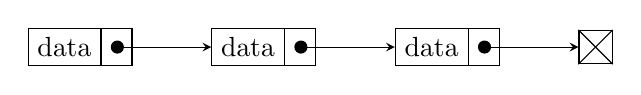
\begin{tikzpicture}[list/.style={rectangle split, rectangle split parts=2,
					draw, rectangle split horizontal}, >=stealth, start chain]
		\node[list,on chain] (A) {data};
		\node[list,on chain] (B) {data};
		\node[list,on chain] (C) {data};
		\node[on chain,draw,inner sep=6pt] (D) {};
		\draw (D.north east) -- (D.south west);
		\draw (D.north west) -- (D.south east);
		\draw[*->] let \p1 = (A.two), \p2 = (A.center) in (\x1,\y2) -- (B);
		\draw[*->] let \p1 = (B.two), \p2 = (B.center) in (\x1,\y2) -- (C);
		\draw[*->] let \p1 = (C.two), \p2 = (C.center) in (\x1,\y2) -- (D);
	\end{tikzpicture}
	\caption{单向链表}
\end{figure}

与数组按照下标来随机寻找元素不同,对于链表的其中一个结点A,只能根据结点A的next指针来找到该结点的下一个结点B,再根据结点B的next指针找到下一个节点C…… \\

数组在内存中的存储方式是顺序存储,链表在内存中的存储方式则是随机存储。链表采用了见缝插针的方式,每一个结点分布在内存的不同位置,依靠next指针关联起来。这样可以灵活有效地利用零散的碎片空间。

\subsection{双向链表(Doubly Linked List)}

那么,通过链表的一个结点,如何能快速找到它的前一个结点呢?要想让每个结点都能回溯到它的前置结点,可以使用双向链表。 \\

双向链表比单向链表稍微复杂一点,它的每一个结点除了拥有data和next指针,还拥有指向前置结点的prev指针。 \\

\begin{figure}[H]
	\centering
	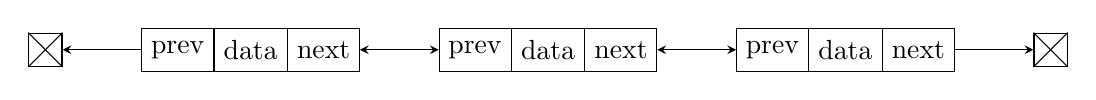
\begin{tikzpicture}[list/.style={rectangle split, rectangle split parts=3,
					draw, rectangle split horizontal}, >=stealth, start chain]
		\node[on chain,draw,inner sep=6pt] (NULL1) {};
		\node[list,on chain] (A) {prev \nodepart{second} data \nodepart{third} next};
		\node[list,on chain] (B) {prev \nodepart{second} data \nodepart{third} next};
		\node[list,on chain] (C) {prev \nodepart{second} data \nodepart{third} next};
		\node[on chain,draw,inner sep=6pt] (NULL2) {};
		\draw (NULL1.north east) -- (NULL1.south west);
		\draw (NULL1.north west) -- (NULL1.south east);
		\draw (NULL2.north east) -- (NULL2.south west);
		\draw (NULL2.north west) -- (NULL2.south east);
		\draw[<-] let \p1 = (A.west), \p2 = (A.center) in (NULL1) -- (\x1,\y2);
		\draw[<->] let \p1 = (A.east), \p2 = (A.center) in (\x1,\y2) -- (B);
		\draw[<->] let \p1 = (B.east), \p2 = (B.center) in (\x1,\y2) -- (C);
		\draw[->] let \p1 = (C.east), \p2 = (C.center) in (\x1,\y2) -- (NULL2);
	\end{tikzpicture}
	\caption{双向链表}
\end{figure}

单向链表只能从头到尾遍历,只能找到后继,无法找到前驱,因此遍历的时候不会死循环。而双向链表需要多分配一个指针的存储空间,每个结点有两个指针,分别指向直接前驱和直接后继。

\subsection{循环链表(Circular Linked List)}

除了单向链表和双向链表以外,还有循环链表。对于单向循环链表,尾结点的next指针指向头结点。对于双向循环链表,尾结点的next指针指向头结点,并且头结点的prev指针指向尾结点。 \\

\begin{figure}[H]
	\centering
	
\begin{tikzpicture}[
			list/.style={
					rectangle split,
					rectangle split parts=2,
					draw,
					rectangle split horizontal
				},
			dotarrow/.style={Circle-Stealth},
			start chain
		]
		\node[list,on chain] (A) {data};
		\node[list,on chain] (B) {data};
		\node[list,on chain] (C) {data};
		\draw[dotarrow] (A.two |- A.center) -- (B);
		\draw[dotarrow] (B.two |- B.center)  -- (C);
		\draw[dotarrow] (C.two |- C.center) to[out=-20,in=190,distance=4cm] (A);
	\end{tikzpicture}
	\caption{单向循环链表}
\end{figure}

\begin{figure}[H]
	\centering
	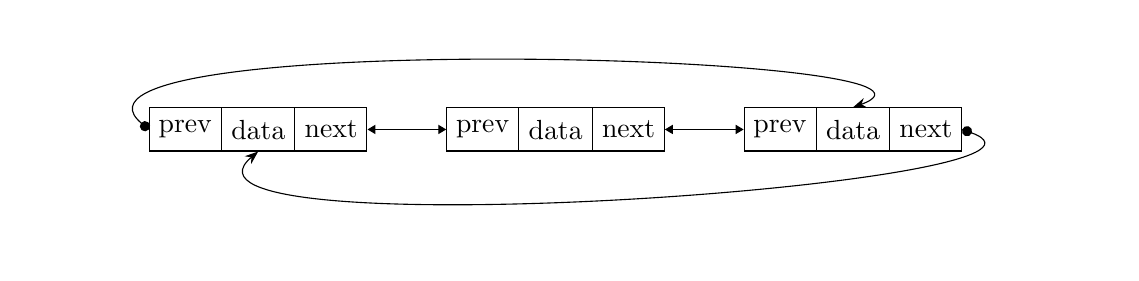
\begin{tikzpicture}[list/.style={
					rectangle split,
					rectangle split parts=3,
					draw,
					rectangle split horizontal
				},
			dotarrow/.style={Circle-Stealth},
			start chain]
		\node[list,on chain] (A) {prev \nodepart{second} data \nodepart{third} next};
		\node[list,on chain] (B) {prev \nodepart{second} data \nodepart{third} next};
		\node[list,on chain] (C) {prev \nodepart{second} data \nodepart{third} next};

		\draw[dotarrow] (A.center -| A.west) to[out=-220,in=20,distance=2cm] (C.north);
		\draw[<->] let \p1 = (A.east), \p2 = (A.center) in (\x1,\y2) -- (B);
		\draw[<->] let \p1 = (B.east), \p2 = (B.center) in (\x1,\y2) -- (C);
		\draw[dotarrow] (C.east |- C.center) to[out=-20,in=220,distance=2cm] (A.south);
	\end{tikzpicture}
	\caption{双向循环链表}
\end{figure}

\newpage

\section{链表的增删改查}

\subsection{查找结点}

在查找元素时,链表不像数组那样可以通过下标快速进行定位,只能从头结点开始向后一个一个结点逐一查找。 \\

链表中的数据只能按顺序进行访问,最坏的时间复杂度是$ O(n) $。 \\

\mybox{查找结点}

\begin{lstlisting}[language=C]
Node* search(List *head, dataType val) {
    // 查找元素位置
    Node *temp = head;
    while(temp) {
        if(temp->data == val) {
            return temp;
        }
        temp = temp->next;
    }
    return NULL;        // 未找到
}
\end{lstlisting}

\subsection{更新结点}

如果不考虑查找结点的过程,链表的更新过程会像数组那样简单,直接把旧数据替换成新数据即可。 \\

\mybox{更新结点}

\begin{lstlisting}[language=C]
void replace(List *head, int pos, dataType val) {
    // 找到元素位置
    Node *temp = head;
    for(int i = 0; i < pos; i++) {
        temp = temp->next;
    }
    temp->data = val;
}
\end{lstlisting}

\subsection{插入结点}

链表插入结点,分为3种情况:

\subsubsection{尾部插入}

把最后一个结点的next指针指向新插入的结点。

\begin{figure}[H]
	\centering
	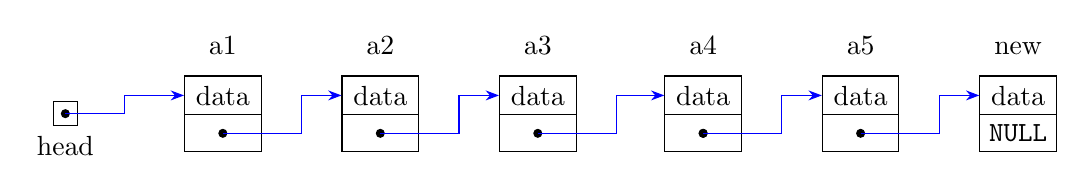
\begin{tikzpicture}[node distance=2cm, auto, scale=1,
			every node/.style={scale=1}]
		\node[head, label=below:head] (head) {};
		\node[data, right of=head] (A) {\data};
		\node[above of=A,node distance=0.5cm,label=above:a1] (a1){};
		\node[data, right of=A] (B) {\data};
		\node[above of=B,node distance=0.5cm,label=above:a2] (a2){};
		\node[data, right of=B] (C) {\data};
		\node[above of=C,node distance=0.5cm,label=above:a3] (a3){};
		\node[data, right of=C, xshift=0.1cm] (D) {\data};%, xshift=1.5cm
		\node[above of=D,node distance=0.5cm,label=above:a4] (a4){};
		\node[data, right of=D] (E) {\data};
		\node[above of=E,node distance=0.5cm,label=above:a5] (a5){};
		\node[data, right of=E] (last) {data \nodepart{second} \texttt{NULL}};
		\node[above of=last,node distance=0.5cm,label=above:new] (new){};

		\draw[fill] (head.center) circle (0.05);

		\path[ptr] (head.center) --++(right:7.5mm) |- (A.text west);
		\draw[fill] ($(A.south)!0.5!(A.text split)$) circle (0.05);
		\draw[ptr] ($(A.south)!0.5!(A.text split)$) --++(right:10mm) |- (B.text west);
		\draw[fill] ($(B.south)!0.5!(B.text split)$) circle (0.05);
		\draw[ptr] ($(B.south)!0.5!(B.text split)$) --++(right:10mm) |- (C.text west);
		\draw[fill] ($(C.south)!0.5!(C.text split)$) circle (0.05);
		\draw[ptr] ($(C.south)!0.5!(C.text split)$) --++(right:10mm) |- (D.text west);
		\draw[fill] ($(D.south)!0.5!(D.text split)$) circle (0.05);

		\draw[fill] ($(D.south)!0.5!(D.text split)$) circle (0.05);
		\draw[ptr] ($(D.south)!0.5!(D.text split)$) --++(right:10mm) |- (E.text west);
		\draw[fill] ($(E.south)!0.5!(E.text split)$) circle (0.05);
		\draw[ptr] ($(E.south)!0.5!(E.text split)$) --++(right:10mm) |- (last.text west);
	\end{tikzpicture}
	\caption{尾部插入}
\end{figure}

\subsubsection{头部插入}

先把新结点的next指针指向原先的头结点,再把新结点设置为链表的头结点。

\begin{figure}[H]
	\centering
	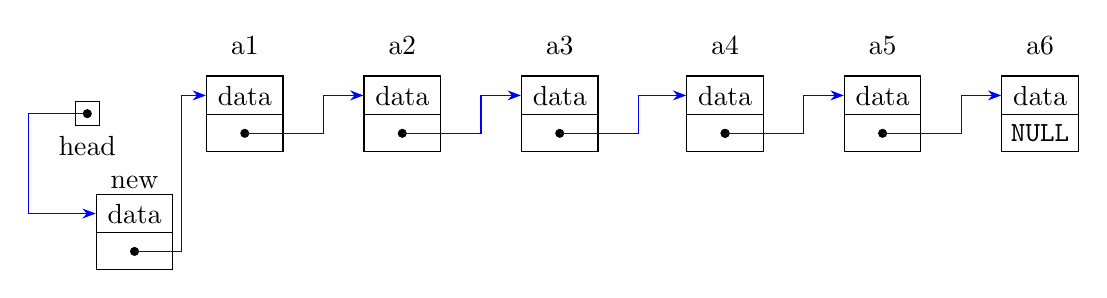
\begin{tikzpicture}[node distance=2cm, auto, scale=1,
			every node/.style={scale=1}]
		\node[head, label=below:head, xshift=-0.5cm] (head) {};
		\node[data, right of=head] (A) {\data};
		\node[above of=A,node distance=0.5cm,label=above:a1] (a1){};
		\node[data, right of=A] (B) {\data};
		\node[above of=B,node distance=0.5cm,label=above:a2] (a2){};
		\node[data, right of=B] (C) {\data};
		\node[above of=C,node distance=0.5cm,label=above:a3] (a3){};
		\node[data, below of=head, xshift=0.6cm, yshift=0.5cm] (NEW) {\data};
		\node[above of=NEW,node distance=0.3cm,label=above:new] (new){};
		\node[data, right of=C, xshift=0.1cm] (D) {\data};%, xshift=1.5cm
		\node[above of=D,node distance=0.5cm,label=above:a4] (a4){};
		\node[data, right of=D] (E) {\data};
		\node[above of=E,node distance=0.5cm,label=above:a5] (a5){};
		\node[data, right of=E] (last) {data \nodepart{second} \texttt{NULL}};
		\node[above of=last,node distance=0.5cm,label=above:a6] (a6){};

		\draw[fill] (head.center) circle (0.05);

		\path[ptr] (head.center) --++(left:7.5mm) |- (NEW.text west);
		\draw[fill] ($(NEW.south)!0.5!(NEW.text split)$) circle (0.05);
		\draw[ptr] ($(NEW.south)!0.5!(NEW.text split)$) --++(right:6mm) |- (A.text west);
		\draw[fill] ($(A.south)!0.5!(A.text split)$) circle (0.05);
		\draw[ptr] ($(A.south)!0.5!(A.text split)$) --++(right:10mm) |- (B.text west);
		\draw[fill] ($(B.south)!0.5!(B.text split)$) circle (0.05);
		\draw[ptr] ($(B.south)!0.5!(B.text split)$) --++(right:10mm) |- (C.text west);
		\draw[fill] ($(C.south)!0.5!(C.text split)$) circle (0.05);
		\draw[ptr] ($(C.south)!0.5!(C.text split)$) --++(right:10mm) |- (D.text west);
		\draw[fill] ($(D.south)!0.5!(D.text split)$) circle (0.05);
		\draw[fill] ($(D.south)!0.5!(D.text split)$) circle (0.05);
		\draw[ptr] ($(D.south)!0.5!(D.text split)$) --++(right:10mm) |- (E.text west);
		\draw[fill] ($(E.south)!0.5!(E.text split)$) circle (0.05);
		\draw[ptr] ($(E.south)!0.5!(E.text split)$) --++(right:10mm) |- (last.text west);
	\end{tikzpicture}
	\caption{头部插入}
\end{figure}

\subsubsection{中间插入}

先把新结点的next指针指向插入位置的结点,再将插入位置的前置结点的next指针指向新结点。

\begin{figure}[H]
	\centering
	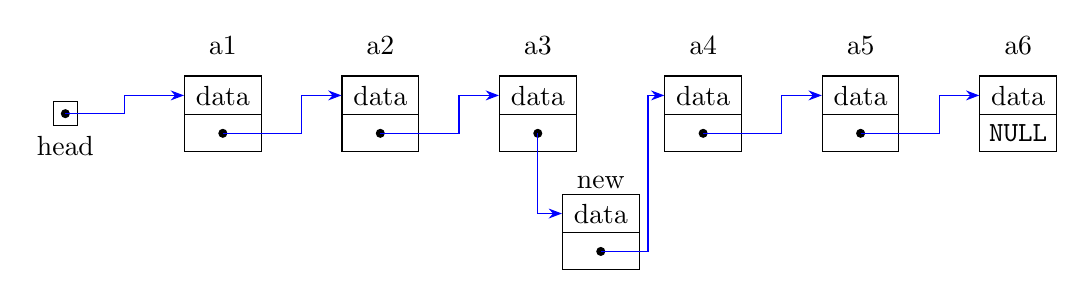
\begin{tikzpicture}[node distance=2cm, auto, scale=1,
			every node/.style={scale=1}]
		\node[head, label=below:head] (head) {};
		\node[data, right of=head] (A) {\data};
		\node[above of=A,node distance=0.5cm,label=above:a1] (a1){};
		\node[data, right of=A] (B) {\data};
		\node[above of=B,node distance=0.5cm,label=above:a2] (a2){};
		\node[data, right of=B] (C) {\data};
		\node[above of=C,node distance=0.5cm,label=above:a3] (a3){};
		\node[data, below of=C, xshift=0.8cm, yshift=0.5cm] (NEW) {\data};
		\node[above of=NEW,node distance=0.3cm,label=above:new] (new){};
		\node[data, right of=C, xshift=0.1cm] (D) {\data};%, xshift=1.5cm
		\node[above of=D,node distance=0.5cm,label=above:a4] (a4){};
		\node[data, right of=D] (E) {\data};
		\node[above of=E,node distance=0.5cm,label=above:a5] (a5){};
		\node[data, right of=E] (last) {data \nodepart{second} \texttt{NULL}};
		\node[above of=last,node distance=0.5cm,label=above:a6] (a6){};

		\draw[fill] (head.center) circle (0.05);

		\path[ptr] (head.center) --++(right:7.5mm) |- (A.text west);
		\draw[fill] ($(A.south)!0.5!(A.text split)$) circle (0.05);
		\draw[ptr] ($(A.south)!0.5!(A.text split)$) --++(right:10mm) |- (B.text west);
		\draw[fill] ($(B.south)!0.5!(B.text split)$) circle (0.05);
		\draw[ptr] ($(B.south)!0.5!(B.text split)$) --++(right:10mm) |- (C.text west);
		\draw[fill] ($(C.south)!0.5!(C.text split)$) circle (0.05);

		\draw[ptr] ($(C.south)!0.5!(C.text split)$) |- (NEW.text west);
		\draw[fill] ($(NEW.south)!0.5!(NEW.text split)$) circle (0.05);
		\draw[ptr] ($(NEW.south)!0.5!(NEW.text split)$) --++(right:6mm) |- (D.text west);
		\draw[fill] ($(D.south)!0.5!(D.text split)$) circle (0.05);
		\draw[ptr] ($(D.south)!0.5!(D.text split)$) --++(right:10mm) |- (E.text west);
		\draw[fill] ($(E.south)!0.5!(E.text split)$) circle (0.05);
		\draw[ptr] ($(E.south)!0.5!(E.text split)$) --++(right:10mm) |- (last.text west);
	\end{tikzpicture}
	\caption{中间插入}
\end{figure}

只要内存空间允许,能够插入链表的元素是无穷无尽的,不需要像数组考虑扩容的问题。如果不考虑插入之前的查找元素的过程,只考虑纯粹的插入操作,时间复杂度是$ O(1) $。

\subsection{删除结点}

链表的删除操作也分3种情况:

\subsubsection{尾部删除}

把倒数第二个结点的next指针指向空。

\begin{figure}[H]
	\centering
	\begin{tikzpicture}[node distance=2cm, auto, scale=1,
			every node/.style={scale=1}]
		\node[head, label=below:head] (head) {};
		\node[data, right of=head] (A) {\data};
		\node[above of=A,node distance=0.5cm,label=above:a1] (a1){};
		\node[data, right of=A] (B) {\data};
		\node[above of=B,node distance=0.5cm,label=above:a2] (a2){};
		\node[data, right of=B] (C) {\data};
		\node[above of=C,node distance=0.5cm,label=above:a3] (a3){};
		\node[data, right of=C, xshift=0.1cm] (D) {\data};
		\node[above of=D,node distance=0.5cm,label=above:a4] (a4){};
		\node[data, right of=D] (E) {\data};
		\node[above of=E,node distance=0.5cm,label=above:a5] (a5){};

		\draw[fill] (head.center) circle (0.05);

		\path[ptr] (head.center) --++(right:7.5mm) |- (A.text west);
		\draw[fill] ($(A.south)!0.5!(A.text split)$) circle (0.05);
		\draw[ptr] ($(A.south)!0.5!(A.text split)$) --++(right:10mm) |- (B.text west);
		\draw[fill] ($(B.south)!0.5!(B.text split)$) circle (0.05);
		\draw[ptr] ($(B.south)!0.5!(B.text split)$) --++(right:10mm) |- (C.text west);
		\draw[fill] ($(C.south)!0.5!(C.text split)$) circle (0.05);
		\draw[ptr] ($(C.south)!0.5!(C.text split)$) --++(right:10mm) |- (D.text west);
		\draw[fill] ($(D.south)!0.5!(D.text split)$) circle (0.05);

		\draw[fill] ($(D.south)!0.5!(D.text split)$) circle (0.05);
		\draw[ptr,red] ($(D.south)!0.5!(D.text split)$) -- (8.1,-1.7) -- (11.5,-1.7) -- (last.text west);
		\draw[fill] ($(E.south)!0.5!(E.text split)$) circle (0.05);

		\draw (12.3,0.3) node {NULL};

		\draw[-, red] (9.3,1) -- (11,-1); 
	\end{tikzpicture}
	\caption{尾部删除}
\end{figure}

\subsubsection{头部删除}

把链表的头结点设置为原先头结点的next指针。

\begin{figure}[H]
	\centering
	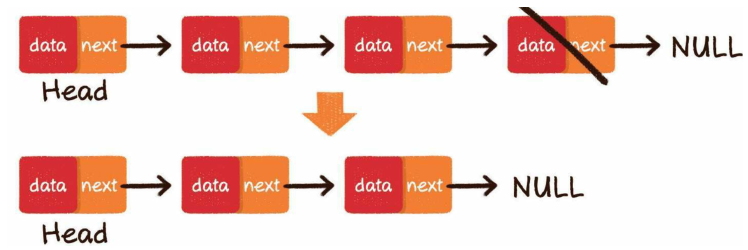
\includegraphics[scale=0.8]{img/C3/3-2/1.png}
\end{figure}

\subsubsection{中间删除}

把要删除的结点的前置结点的next指针,指向要删除结点的下一个结点。

\begin{figure}[H]
	\centering
	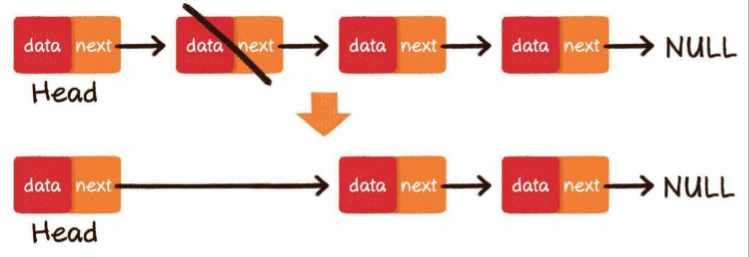
\includegraphics[scale=0.5]{img/C3/3-2/2.png}
\end{figure}

许多高级语言,如Java,拥有自动化的垃圾回收机制,所以不用刻意去释放被删除的结点,只要没有外部引用指向它们,被删除的结点会被自动回收。 \\

如果不考虑删除操作之前的查找的过程,只考虑纯粹的删除操作,时间复杂度是$ O(1) $。

\newpage

\section{带头结点的链表}

\subsection{带头结点的链表}

为了方便链表的插入、删除操作,在链表加上头结点之后,无论链表是否为空,头指针始终指向头结尾。因此对于空表和非空表的处理也统一了,方便了链表的操作,也减少了程序的复杂性和出现bug的机会。 \\

\mybox{插入结点}

\begin{lstlisting}[language=C]
void insert(List *head, int pos, dataType val) {
    Node *newNode = (Node *)malloc(sizeof(Node));
    newNode->data = val;
    newNode->next =  NULL;
    
    // 找到插入位置
    Node *temp = head;
    for(int i = 0; i < pos; i++) {
        temp = temp->next;
    }
    newNode->next = temp->next;
    temp->next = newNode;
}
\end{lstlisting}

\vspace{0.5cm}

\mybox{删除结点}

\begin{lstlisting}[language=C]
void delete(List *head, int pos) {
    Node *temp = head;
    for(int i = 0; i < pos; i++) {
        temp = temp->next;
    }
    Node *del = temp->next;
    temp->next = del->next;
    free(del);
    del = NULL;
}
\end{lstlisting}

\subsection{数组VS链表}

数据结构没有绝对的好与坏,数组和链表各有千秋。

\begin{table}[H]
	\centering
	\setlength{\tabcolsep}{5mm}{
		\begin{tabular}{|c|l|l|}
			\hline
			\textbf{比较内容} & \textbf{数组}          & \textbf{链表}                \\
			\hline
			基本              & 一组固定数量的数据项   & 可变数量的数据项             \\
			\hline
			大小              & 声明期间指定           & 无需指定,执行期间增长或收缩 \\
			\hline
			存储分配          & 元素位置在编译期间分配 & 元素位置在运行时分配         \\
			\hline
			元素顺序          & 连续存储               & 随机存储                     \\
			\hline
			访问元素          & 直接访问:索引、下标   & 顺序访问:指针遍历           \\
			\hline
			插入/删除         & 速度慢                 & 快速、高效                   \\
			\hline
			查找              & 线性查找、二分查找     & 线性查找                     \\
			\hline
			内存利用率        & 低效                   & 高效                         \\
			\hline
		\end{tabular}
	}
	\caption{数组VS链表}
\end{table}

数组的优势在于能够快速定位元素,对于读操作多、写操作少的场景来说,用数组更合适一些。 \\

相反,链表的优势在于能够灵活地进行插入和删除操作,如果需要频繁地插入、删除元素,用链表更合适一些。
% \chapter{栈}

\section{栈}

\subsection{栈(Stack)}

栈,又名堆栈,是一种运算受限的线性数据结构,栈只能在表尾进行插入和删除操作。 \\

栈中的元素只能先进后出(FILO, First In Last Out)。最早进入栈的元素所存放的位置叫作栈底(bottom),最后进入栈的元素存放的位置叫作栈顶(top)。 \\

\begin{figure}[H]
    \centering
    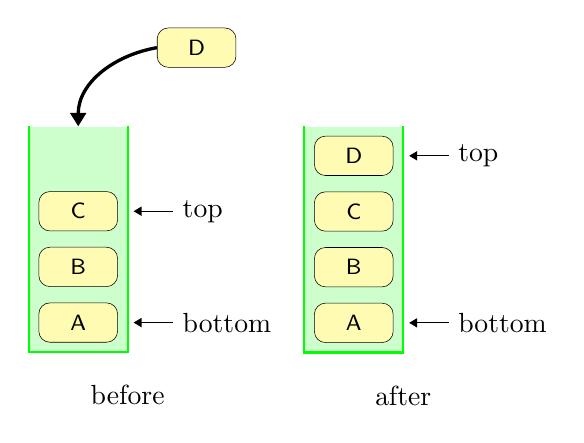
\begin{tikzpicture}
        \matrix[queue] (Q1) {
        |[fill=none, draw=none]| \\
        |(front)| C\\
        B\\
        |(rear)| A\\};
        \draw[green,thick,-] (Q1.north west) |-(Q1.south)-| (Q1.north east);
        \draw[<-] ([xshift=.2cm]front.east) -- ++ (0:.5) node[right] {top};
        \draw[<-] ([xshift=.2cm]rear.east) -- ++ (0:.5) node[right] {bottom};
        \draw[<-,very thick] (Q1.north) to[out=90,in=190] ++ (1,1) node[right, queue element] (D) {D};
        \node[below=3mm of Q1.south east] {before};

        \scope[xshift=3.5cm]
        \matrix[queue] (Q1) {
            |(front)| D \\
            C           \\
            B           \\
            |(rear)| A\\};
        \draw[green,thick,-] (Q1.north west) |-(Q1.south)-| (Q1.north east);
        \draw[<-] ([xshift=.2cm]front.east) -- ++ (0:.5) node[right] {top};
        \draw[<-] ([xshift=.2cm]rear.east) -- ++ (0:.5) node[right] {bottom};
        \node[below=3mm of Q1.south east] {after};
        \endscope
    \end{tikzpicture}
    \caption{栈}
\end{figure}

栈这种数据结构既可以用数组来实现,也可以用链表来实现。

\subsection{顺序栈}

使用数组方式实现的栈称为静态栈。可以根据下标来表示栈顶在数组中的位置,对于空栈,栈顶为-1。 \\

进行入栈操作时,栈顶指针+1;出栈时,栈顶指针-1。 \\

\begin{figure}[H]
    \centering
    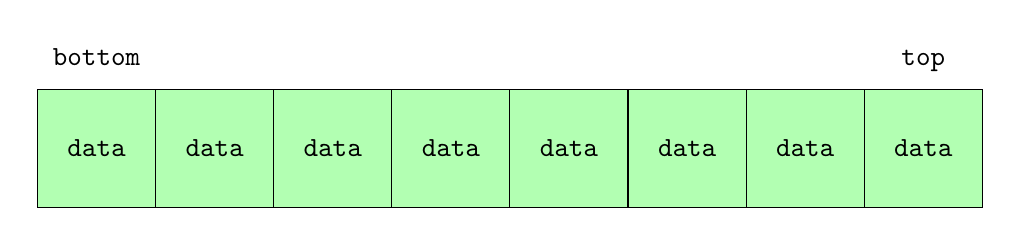
\begin{tikzpicture}[font=\ttfamily,
            array/.style={matrix of nodes,nodes={draw, minimum size=15mm, fill=green!30},column sep=-\pgflinewidth, row sep=0.5mm, nodes in empty cells,
                    row 1/.style={nodes={draw=none, fill=none, minimum size=5mm}},
                }]

        \matrix[array] (array) {
            bottom &      &      &      &      &      &      & top  \\
            data   & data & data & data & data & data & data & data \\
        };
    \end{tikzpicture}
    \caption{顺序栈}
\end{figure}

对满栈进行入栈和对空栈进行出栈操作操作都会产生数组的越界并引起程序崩溃,称为上溢和下溢。因此使用顺序栈前需要提前声明一个数组的大小,如果数组大小不够则可能发生数组越界,如果数组太大则会浪费一定的空间。 \\

使用数组实现的栈的执行效率会比用链表来实现的高,入栈和出栈不需要移动大量元素,只需要移动栈顶指针即可。 \\

\subsection{链式栈}

使用链表方式实现的栈称为动态栈。通过在表头插入一个元素来实现入栈,通过删除表尾元素来实现出栈。 \\

\begin{figure}[H]
    \centering
    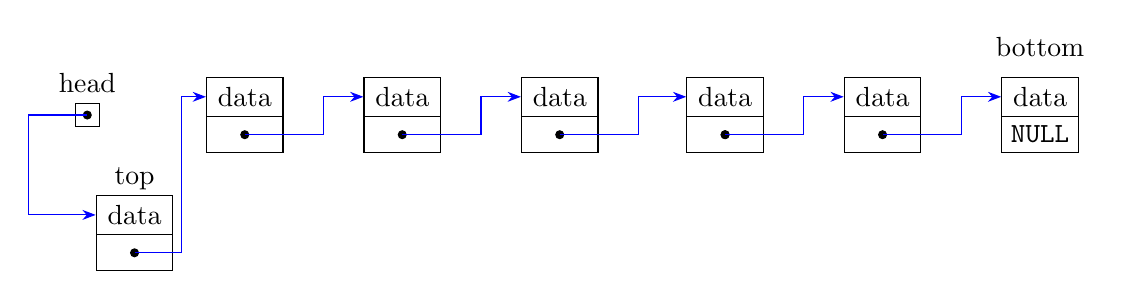
\begin{tikzpicture}[node distance=2cm, auto, scale=1,
            every node/.style={scale=1}]
        \node[head, label=above:head, xshift=-0.5cm] (head) {};
        \node[data, right of=head] (A) {\data};
        \node[above of=A,node distance=0.5cm] (a1){};
        \node[data, right of=A] (B) {\data};
        \node[above of=B,node distance=0.5cm] (a2){};
        \node[data, right of=B] (C) {\data};
        \node[above of=C,node distance=0.5cm] (a3){};
        \node[data, below of=head, xshift=0.6cm, yshift=0.5cm] (NEW) {\data};
        \node[above of=NEW,node distance=0.3cm,label=above:top] (new){};
        \node[data, right of=C, xshift=0.1cm] (D) {\data};%, xshift=1.5cm
        \node[above of=D,node distance=0.5cm] (a4){};
        \node[data, right of=D] (E) {\data};
        \node[above of=E,node distance=0.5cm] (a5){};
        \node[data, right of=E] (last) {data \nodepart{second} \texttt{NULL}};
        \node[above of=last,node distance=0.5cm,label=above:bottom] (a6){};

        \draw[fill] (head.center) circle (0.05);

        \path[ptr] (head.center) --++(left:7.5mm) |- (NEW.text west);
        \draw[fill] ($(NEW.south)!0.5!(NEW.text split)$) circle (0.05);
        \draw[ptr] ($(NEW.south)!0.5!(NEW.text split)$) --++(right:6mm) |- (A.text west);
        \draw[fill] ($(A.south)!0.5!(A.text split)$) circle (0.05);
        \draw[ptr] ($(A.south)!0.5!(A.text split)$) --++(right:10mm) |- (B.text west);
        \draw[fill] ($(B.south)!0.5!(B.text split)$) circle (0.05);
        \draw[ptr] ($(B.south)!0.5!(B.text split)$) --++(right:10mm) |- (C.text west);
        \draw[fill] ($(C.south)!0.5!(C.text split)$) circle (0.05);
        \draw[ptr] ($(C.south)!0.5!(C.text split)$) --++(right:10mm) |- (D.text west);
        \draw[fill] ($(D.south)!0.5!(D.text split)$) circle (0.05);
        \draw[fill] ($(D.south)!0.5!(D.text split)$) circle (0.05);
        \draw[ptr] ($(D.south)!0.5!(D.text split)$) --++(right:10mm) |- (E.text west);
        \draw[fill] ($(E.south)!0.5!(E.text split)$) circle (0.05);
        \draw[ptr] ($(E.south)!0.5!(E.text split)$) --++(right:10mm) |- (last.text west);
    \end{tikzpicture}
    \caption{链式栈}
\end{figure}

动态栈有链表的部分特性,元素与元素之间在物理存储上可以不连续,但是功能有些受限制,动态栈只能在栈顶处进行插入和删除操作,不能在栈尾或栈中间进行插入和删除操作。 \\

动态栈的元素内存是动态分配的,避免了静态栈可能会浪费空间的问题,但是对申请和释放空间的调用开销会比较大。

\subsection{栈的应用}

栈的输出顺序和输入顺序相反,所以栈同行用于对历史的回溯。例如实现递归的逻辑,就可以用栈回溯调用链。 \\

\begin{figure}[H]
    \centering
    \begin{drawstack}
        \startframe
        \cell{N = 1}
        \cell{...}
        \finishframe{fact(1)}
        \startframe
        \cell{N = 2}
        \cell{...}
        \finishframe{fact(2)}
        \cell{$ \vdots $}
        \startframe
        \cell{N = 5}
        \cell{...}
        \finishframe{fact(5)}
    \end{drawstack}
    \caption{函数调用栈}
\end{figure}

栈还有一个著名的应用场景就是面包屑导航,使用户在流浪页面时可以轻松地回溯到上一级更更上一级页面。

\begin{figure}[H]
    \centering
    
\includegraphics[]{img/C4/4-1/1.png}
    \caption{面包屑导航}
\end{figure}

\newpage

\section{入栈与出栈}

\subsection{入栈(Push)}

入栈操作就是把新元素放入栈中,只允许从栈顶一侧放入元素,新元素的位置将会成为新的栈顶。最初,栈为空,栈顶的初始值为-1。每当向栈中添加元素时,栈顶指针+1。 \\

入栈只影响最后一个元素,不涉及元素的整体移动,所以无论是以数组还是链表实现,时间复杂度都是$ O(1) $。 \\

\mybox{入栈}

\begin{lstlisting}[language=C]
void push(Stack *stack, dataType val) {
    stack->data[++stack->top] = val;
}
\end{lstlisting}

\subsection{出栈(Pop)}

出栈操作就是把新元素从栈中弹出,只有栈顶元素才允许出栈,出栈元素的前一个元素将会成为新的栈顶。从栈中移出元素,栈顶指针-1。数组中元素的删除并非真正意义上把元素从内存中清除,出栈只需对栈顶-1即可,后期向栈中添加元素时,新元素会将旧元素覆盖。 \\

出栈只影响最后一个元素,不涉及元素的整体移动,所以无论是以数组还是链表实现,时间复杂度都是$ O(1) $。 \\

\mybox{出栈}

\begin{lstlisting}[language=C]
dataType pop(Stack *stack) {
    return stack->data[stack->top--];
}
\end{lstlisting}

\newpage

\section{最小栈}

\subsection{最小栈}

设计一个支持push()、pop()、peek()和getMin()操作的栈,并能在常数时间内检索到最小元素。 \\

对于栈来说,如果一个元素a在入栈时,栈里有其它的元素b、c、d,那么无论这个栈在之后经历了什么操作,只要a在栈中,b、c、d就一定在栈中。因此,在操作过程中的任意一个时刻,只要栈顶的元素是a,那么就可以确定栈里面现在的元素一定是a、b、c、d。 \\

那么可以在每个元素a入栈时把当前栈的最小值m存储起来。在这之后无论何时,如果栈顶元素是a,就可以直接返回存储的最小值m。 \\

当一个元素要入栈时,取辅助栈的栈顶存储的最小值,与当前元素比较得出最小值,将这个最小值插入辅助栈中。当一个元素要出栈时,把辅助栈的栈顶元素也一并弹出。这样在任意一个时刻,栈内元素的最小值就存储在辅助栈的栈顶元素中。 \\

\mybox{最小栈}

\begin{lstlisting}[language=Python]
class MinStack:
    def __init__(self):
        self.stack = []
        self.min_stack = [math.inf]
    
    def push(self, data):
        self.stack.append(data)
        self.min_stack.append(min(data, self.min_stack[-1]))
    
    def pop(self):
        self.stack.pop()
        self.min_stack.pop()
    
    def peek(self):
        return self.stack[-1]
    
    def get_min(self):
        return self.min_stack[-1]
\end{lstlisting}

\newpage

\section{括号匹配}

\subsection{括号匹配}

给定一个只包括"("、")"、"["、"]"、"\{"和"\}"的字符串,判断字符串是否有效。有效字符串需满足左括号必须用相同类型的右括号闭合,并且左括号必须以正确的顺序闭合。 \\

判断括号的有效性可以使用栈来解决。通过遍历字符串,当遇到左括号时,会期望在后续的遍历中,有一个相同类型的右括号将其闭合。由于后遇到的左括号要先闭合,因此将这个左括号放入栈顶。 \\

当遇到右括号时,需要将一个相同类型的左括号闭合。此时可以取出栈顶的左括号并判断它们是否是相同类型的括号。如果不是相同的类型,或者栈中并没有左括号,那么字符串无效。在遍历结束后,如果为空栈,说明字符串中的所有左括号闭合。 \\

注意有效字符串的长度一定为偶数,因此如果字符串的长度为奇数,可以直接返回判断出字符串无效,省去后续的遍历判断过程。 \\

\mybox{括号匹配}

\begin{lstlisting}[language=Python]
def valid_paratheses(s):
    if len(s) % 2 == 1:
        return False
    
    pairs = {")": "(", "]": "[", "}": "{"}
    stack = list()
    for paran in s:
        if paran in pairs:
            if not stack or stack[-1] != pairs[paran]:
                return False
            stack.pop()
        else:
            stack.append(paran)

    return not stack
\end{lstlisting}

\newpage

\section{表达式求值}

\subsection{表达式求值}

逆波兰表达式是一种后缀表达式,所谓后缀就是指运算符写在运算数的后面。平常使用的算式则是一种中缀表达式,如$ (1 + 2) * (3 + 4) $,该算式的逆波兰表达式写法为$ 1\ 2 + 3\ 4 + * $。 \\

逆波兰表达式的优点在于去掉了中缀表达式中的括号后表达式无歧义,因此适合用栈操作运算。遇到数字则入栈,遇到算符则取出栈顶两个数字进行计算,并将结果压入栈中。 \\

在对中缀表达式求值时,一般都会将其转换为后缀表达式的形式,转换过程同样需要用到栈,规则如下:

\begin{enumerate}
    \item 如果遇到操作数,就直接将其输出。

    \item 如果遇到左括号,将其放入栈中。

    \item 如果遇到右括号,则一直出栈并输出,直到遇到左括号为止。注意,左括号只出栈并不输出。

    \item 如果遇到任何其它的运算符,如果为栈为空,则直接入栈。否则从栈中出栈元素并输出,直到遇到优先级更低的元素(或者栈为空)位置。在出栈完这些元素后,再将当前遇到的运算符入栈。有一点需要注意,只有在遇到右括号的情况下才将左括号出栈,其它情况都不会出栈左括号。

    \item 如果读取到了表达式的末尾,则将栈中所有元素依次出栈输出。
\end{enumerate}

\begin{figure}[H]
    \centering
    \begin{tikzpicture}[]
        \draw[-] (0,0) rectangle (7,1);
        \draw[-] (1,0) -- (1,1);
        \draw[-] (2,0) -- (2,1);
        \draw[-] (3,0) -- (3,1);
        \draw[-] (4,0) -- (4,1);
        \draw[-] (5,0) -- (5,1);
        \draw[-] (6,0) -- (6,1);
        \draw[-] (7,0) -- (7,1);

        \draw (0.5,0.5) node{1};
        \draw (1.5,0.5) node{*};
        \draw (2.5,0.5) node{(};
        \draw (3.5,0.5) node{2};
        \draw (4.5,0.5) node{+};
        \draw (5.5,0.5) node{3};
        \draw (6.5,0.5) node{)};

        \draw[-] (8,3) rectangle (9,-2);
        \draw[-] (8,2) -- (9,2);
        \draw[-] (8,1) -- (9,1);
        \draw[-] (8,0) -- (9,0);
        \draw[-] (8,-1) -- (9,-1);
        \draw (8.5,-2.5) node{num};

        \draw[-] (10,3) rectangle (11,-2);
        \draw[-] (10,2) -- (11,2);
        \draw[-] (10,1) -- (11,1);
        \draw[-] (10,0) -- (11,0);
        \draw[-] (10,-1) -- (11,-1);
        \draw (10.5,-2.5) node{op};

        \draw (8.5,-1.5) node{1};
        \draw[->, red] (0.5,0) to[bend right] (8,-1.5);
    \end{tikzpicture}
\end{figure}

\begin{figure}[H]
    \centering
    \begin{tikzpicture}[]
        \draw[-] (0,0) rectangle (7,1);
        \draw[-] (1,0) -- (1,1);
        \draw[-] (2,0) -- (2,1);
        \draw[-] (3,0) -- (3,1);
        \draw[-] (4,0) -- (4,1);
        \draw[-] (5,0) -- (5,1);
        \draw[-] (6,0) -- (6,1);
        \draw[-] (7,0) -- (7,1);

        \draw (0.5,0.5) node{1};
        \draw (1.5,0.5) node{*};
        \draw (2.5,0.5) node{(};
        \draw (3.5,0.5) node{2};
        \draw (4.5,0.5) node{+};
        \draw (5.5,0.5) node{3};
        \draw (6.5,0.5) node{)};

        \draw[-] (8,3) rectangle (9,-2);
        \draw[-] (8,2) -- (9,2);
        \draw[-] (8,1) -- (9,1);
        \draw[-] (8,0) -- (9,0);
        \draw[-] (8,-1) -- (9,-1);
        \draw (8.5,-2.5) node{num};

        \draw[-] (10,3) rectangle (11,-2);
        \draw[-] (10,2) -- (11,2);
        \draw[-] (10,1) -- (11,1);
        \draw[-] (10,0) -- (11,0);
        \draw[-] (10,-1) -- (11,-1);
        \draw (10.5,-2.5) node{op};

        \draw (8.5,-1.5) node{1};
        \draw (10.5,-1.5) node{*};
        \draw[->, red] (1.5,0) to[bend right] (10,-1.5);
    \end{tikzpicture}
\end{figure}

\begin{figure}[H]
    \centering
    \begin{tikzpicture}[]
        \draw[-] (0,0) rectangle (7,1);
        \draw[-] (1,0) -- (1,1);
        \draw[-] (2,0) -- (2,1);
        \draw[-] (3,0) -- (3,1);
        \draw[-] (4,0) -- (4,1);
        \draw[-] (5,0) -- (5,1);
        \draw[-] (6,0) -- (6,1);
        \draw[-] (7,0) -- (7,1);

        \draw (0.5,0.5) node{1};
        \draw (1.5,0.5) node{*};
        \draw (2.5,0.5) node{(};
        \draw (3.5,0.5) node{2};
        \draw (4.5,0.5) node{+};
        \draw (5.5,0.5) node{3};
        \draw (6.5,0.5) node{)};

        \draw[-] (8,3) rectangle (9,-2);
        \draw[-] (8,2) -- (9,2);
        \draw[-] (8,1) -- (9,1);
        \draw[-] (8,0) -- (9,0);
        \draw[-] (8,-1) -- (9,-1);
        \draw (8.5,-2.5) node{num};

        \draw[-] (10,3) rectangle (11,-2);
        \draw[-] (10,2) -- (11,2);
        \draw[-] (10,1) -- (11,1);
        \draw[-] (10,0) -- (11,0);
        \draw[-] (10,-1) -- (11,-1);
        \draw (10.5,-2.5) node{op};

        \draw (8.5,-1.5) node{1};
        \draw (10.5,-1.5) node{*};
        \draw (10.5,-0.5) node{(};
        \draw[->, red] (2.5,0) to[bend right] (10,-0.5);
    \end{tikzpicture}
\end{figure}

\begin{figure}[H]
    \centering
    \begin{tikzpicture}[]
        \draw[-] (0,0) rectangle (7,1);
        \draw[-] (1,0) -- (1,1);
        \draw[-] (2,0) -- (2,1);
        \draw[-] (3,0) -- (3,1);
        \draw[-] (4,0) -- (4,1);
        \draw[-] (5,0) -- (5,1);
        \draw[-] (6,0) -- (6,1);
        \draw[-] (7,0) -- (7,1);

        \draw (0.5,0.5) node{1};
        \draw (1.5,0.5) node{*};
        \draw (2.5,0.5) node{(};
        \draw (3.5,0.5) node{2};
        \draw (4.5,0.5) node{+};
        \draw (5.5,0.5) node{3};
        \draw (6.5,0.5) node{)};

        \draw[-] (8,3) rectangle (9,-2);
        \draw[-] (8,2) -- (9,2);
        \draw[-] (8,1) -- (9,1);
        \draw[-] (8,0) -- (9,0);
        \draw[-] (8,-1) -- (9,-1);
        \draw (8.5,-2.5) node{num};

        \draw[-] (10,3) rectangle (11,-2);
        \draw[-] (10,2) -- (11,2);
        \draw[-] (10,1) -- (11,1);
        \draw[-] (10,0) -- (11,0);
        \draw[-] (10,-1) -- (11,-1);
        \draw (10.5,-2.5) node{op};

        \draw (8.5,-1.5) node{1};
        \draw (10.5,-1.5) node{*};
        \draw (10.5,-0.5) node{(};
        \draw (8.5,-0.5) node{2};
        \draw[->, red] (3.5,0) to[bend right] (8,-0.5);
    \end{tikzpicture}
\end{figure}

\begin{figure}[H]
    \centering
    \begin{tikzpicture}[]
        \draw[-] (0,0) rectangle (7,1);
        \draw[-] (1,0) -- (1,1);
        \draw[-] (2,0) -- (2,1);
        \draw[-] (3,0) -- (3,1);
        \draw[-] (4,0) -- (4,1);
        \draw[-] (5,0) -- (5,1);
        \draw[-] (6,0) -- (6,1);
        \draw[-] (7,0) -- (7,1);

        \draw (0.5,0.5) node{1};
        \draw (1.5,0.5) node{*};
        \draw (2.5,0.5) node{(};
        \draw (3.5,0.5) node{2};
        \draw (4.5,0.5) node{+};
        \draw (5.5,0.5) node{3};
        \draw (6.5,0.5) node{)};

        \draw[-] (8,3) rectangle (9,-2);
        \draw[-] (8,2) -- (9,2);
        \draw[-] (8,1) -- (9,1);
        \draw[-] (8,0) -- (9,0);
        \draw[-] (8,-1) -- (9,-1);
        \draw (8.5,-2.5) node{num};

        \draw[-] (10,3) rectangle (11,-2);
        \draw[-] (10,2) -- (11,2);
        \draw[-] (10,1) -- (11,1);
        \draw[-] (10,0) -- (11,0);
        \draw[-] (10,-1) -- (11,-1);
        \draw (10.5,-2.5) node{op};

        \draw (8.5,-1.5) node{1};
        \draw (10.5,-1.5) node{*};
        \draw (10.5,-0.5) node{(};
        \draw (8.5,-0.5) node{2};
        \draw (10.5,0.5) node{+};
        \draw[->, red] (4.5,0) to[bend right] (10,0.5);
    \end{tikzpicture}
\end{figure}

\begin{figure}[H]
    \centering
    \begin{tikzpicture}[]
        \draw[-] (0,0) rectangle (7,1);
        \draw[-] (1,0) -- (1,1);
        \draw[-] (2,0) -- (2,1);
        \draw[-] (3,0) -- (3,1);
        \draw[-] (4,0) -- (4,1);
        \draw[-] (5,0) -- (5,1);
        \draw[-] (6,0) -- (6,1);
        \draw[-] (7,0) -- (7,1);

        \draw (0.5,0.5) node{1};
        \draw (1.5,0.5) node{*};
        \draw (2.5,0.5) node{(};
        \draw (3.5,0.5) node{2};
        \draw (4.5,0.5) node{+};
        \draw (5.5,0.5) node{3};
        \draw (6.5,0.5) node{)};

        \draw[-] (8,3) rectangle (9,-2);
        \draw[-] (8,2) -- (9,2);
        \draw[-] (8,1) -- (9,1);
        \draw[-] (8,0) -- (9,0);
        \draw[-] (8,-1) -- (9,-1);
        \draw (8.5,-2.5) node{num};

        \draw[-] (10,3) rectangle (11,-2);
        \draw[-] (10,2) -- (11,2);
        \draw[-] (10,1) -- (11,1);
        \draw[-] (10,0) -- (11,0);
        \draw[-] (10,-1) -- (11,-1);
        \draw (10.5,-2.5) node{op};

        \draw (8.5,-1.5) node{1};
        \draw (10.5,-1.5) node{*};
        \draw (10.5,-0.5) node{(};
        \draw (8.5,-0.5) node{2};
        \draw (10.5,0.5) node{+};
        \draw (8.5,0.5) node{3};
        \draw[->, red] (5.5,1) to[bend left] (8,0.5);
    \end{tikzpicture}
\end{figure}

\begin{figure}[H]
    \centering
    \begin{tikzpicture}[]
        \draw[-] (0,0) rectangle (7,1);
        \draw[-] (1,0) -- (1,1);
        \draw[-] (2,0) -- (2,1);
        \draw[-] (3,0) -- (3,1);
        \draw[-] (4,0) -- (4,1);
        \draw[-] (5,0) -- (5,1);
        \draw[-] (6,0) -- (6,1);
        \draw[-] (7,0) -- (7,1);

        \draw (0.5,0.5) node{1};
        \draw (1.5,0.5) node{*};
        \draw (2.5,0.5) node{(};
        \draw (3.5,0.5) node{2};
        \draw (4.5,0.5) node{+};
        \draw (5.5,0.5) node{3};
        \draw (6.5,0.5) node{)};

        \draw[-] (8,3) rectangle (9,-2);
        \draw[-] (8,2) -- (9,2);
        \draw[-] (8,1) -- (9,1);
        \draw[-] (8,0) -- (9,0);
        \draw[-] (8,-1) -- (9,-1);
        \draw (8.5,-2.5) node{num};

        \draw[-] (10,3) rectangle (11,-2);
        \draw[-] (10,2) -- (11,2);
        \draw[-] (10,1) -- (11,1);
        \draw[-] (10,0) -- (11,0);
        \draw[-] (10,-1) -- (11,-1);
        \draw (10.5,-2.5) node{op};

        \draw (8.5,-1.5) node{1};
        \draw (10.5,-1.5) node{*};
        \draw (10.5,-0.5) node{(};
        \draw (8.5,-0.5) node{2};
        \draw (10.5,0.5) node{+};
        \draw (8.5,0.5) node{3};
        \draw[->, red] (6.5,2) -- (6.5,1);
        \draw[->, red] (10,0.5) -- (9,1.5);
        \draw[->, red] (11,-0.5) -- (12,-0.5);
    \end{tikzpicture}
\end{figure}

\begin{figure}[H]
    \centering
    \begin{tikzpicture}[]
        \draw[-] (0,0) rectangle (7,1);
        \draw[-] (1,0) -- (1,1);
        \draw[-] (2,0) -- (2,1);
        \draw[-] (3,0) -- (3,1);
        \draw[-] (4,0) -- (4,1);
        \draw[-] (5,0) -- (5,1);
        \draw[-] (6,0) -- (6,1);
        \draw[-] (7,0) -- (7,1);

        \draw (0.5,0.5) node{1};
        \draw (1.5,0.5) node{*};
        \draw (2.5,0.5) node{(};
        \draw (3.5,0.5) node{2};
        \draw (4.5,0.5) node{+};
        \draw (5.5,0.5) node{3};
        \draw (6.5,0.5) node{)};

        \draw[-] (8,3) rectangle (9,-2);
        \draw[-] (8,2) -- (9,2);
        \draw[-] (8,1) -- (9,1);
        \draw[-] (8,0) -- (9,0);
        \draw[-] (8,-1) -- (9,-1);
        \draw (8.5,-2.5) node{num};

        \draw[-] (10,3) rectangle (11,-2);
        \draw[-] (10,2) -- (11,2);
        \draw[-] (10,1) -- (11,1);
        \draw[-] (10,0) -- (11,0);
        \draw[-] (10,-1) -- (11,-1);
        \draw (10.5,-2.5) node{op};

        \draw (8.5,-1.5) node{1};
        \draw (10.5,-1.5) node{*};
        \draw (8.5,-0.5) node{2};
        \draw (8.5,0.5) node{3};
        \draw (8.5,1.5) node{+};
        \draw[->, red] (10,-1.5) -- (9,2.5);
    \end{tikzpicture}
\end{figure}

\begin{figure}[H]
    \centering
    \begin{tikzpicture}[]
        \draw[-] (0,0) rectangle (7,1);
        \draw[-] (1,0) -- (1,1);
        \draw[-] (2,0) -- (2,1);
        \draw[-] (3,0) -- (3,1);
        \draw[-] (4,0) -- (4,1);
        \draw[-] (5,0) -- (5,1);
        \draw[-] (6,0) -- (6,1);
        \draw[-] (7,0) -- (7,1);

        \draw (0.5,0.5) node{1};
        \draw (1.5,0.5) node{*};
        \draw (2.5,0.5) node{(};
        \draw (3.5,0.5) node{2};
        \draw (4.5,0.5) node{+};
        \draw (5.5,0.5) node{3};
        \draw (6.5,0.5) node{)};

        \draw[-] (8,3) rectangle (9,-2);
        \draw[-] (8,2) -- (9,2);
        \draw[-] (8,1) -- (9,1);
        \draw[-] (8,0) -- (9,0);
        \draw[-] (8,-1) -- (9,-1);
        \draw (8.5,-2.5) node{num};

        \draw[-] (10,3) rectangle (11,-2);
        \draw[-] (10,2) -- (11,2);
        \draw[-] (10,1) -- (11,1);
        \draw[-] (10,0) -- (11,0);
        \draw[-] (10,-1) -- (11,-1);
        \draw (10.5,-2.5) node{op};

        \draw (8.5,-1.5) node{1};
        \draw (8.5,-0.5) node{2};
        \draw (8.5,0.5) node{3};
        \draw (8.5,1.5) node{+};
        \draw (8.5,2.5) node{*};
    \end{tikzpicture}
\end{figure}

\mybox{表达式求值}

\begin{lstlisting}[language=Python]
def priority(op):
    """
        运算符的优先级
        乘除法优先级高于加减法
        Args:
            op (str): 运算符
        Returns:
            (int): 优先级
    """
    if op == "*" or op == "/":
        return 2
    elif op == "+" or op == "-":
        return 1
    else:
        return 0

def infix_to_postfix(exp):
    """
        中缀表达式转换后缀表达式
        转换后的后缀表达式操作数之前带空格
        Args:
            exp (str): 中缀表达式
        Returns:
            (str): 后缀表达式
    """
    postfix = ""    # 保存生成的后缀表达式
    s = stack.Stack()

    number = ""
    for ch in exp:
        # 如果是数字,保存每一位数字
        if ch.isdigit():
            number += ch
            continue
        
        # 如果读取一个完整数字,直接输出
        if len(number) > 0:
            postfix += number + " "
            number = ""
        
        # 空格忽略
        if ch == " ":
            continue
        
        # 如果是运算符,并且空栈,则直接入栈
        if s.is_empty():
            s.push(ch)
        # 如果遇到左括号,将其放入栈中
        elif ch == "(":
            s.push(ch)
        # 如果遇到右括号,则一直出栈并输出,直到遇到左括号为止
        # 注意,左括号只出栈并不输出
        elif ch == ")":
            while s.peek() != "(":
                postfix += s.pop() + " "
            s.pop()
        # 如果遇到任何其它的运算符,如果为栈为空,则直接入栈
        # 否则从栈中出栈元素并输出,直到遇到优先级更低的元素(或为空)
        # 在出栈完这些元素后,再将当前遇到的运算符入栈
        # 只有遇到右括号的情况下才将左括号出栈
        else:
            while not s.is_empty() 
                    and priority(ch) <= priority(s.peek()):
                postfix += s.pop() + " "
            s.push(ch)
    
    # 如果读取一个完整数字,直接输出
    if len(number) > 0:
        postfix += number + " "
        number = ""
    
    while not s.is_empty():
        postfix += s.pop() + " "
    
    return postfix.rstrip()

def calculate(postfix):
    """
    表达式求值
    Args:
        postfix (str): 后缀表达式
    Returns:
        (int): 表达式结果
    """
    s = stack.Stack()

    tokens = postfix.split()
    for token in tokens:
        # 数字则入栈
        try:
            s.push(int(token))
        # 运算符则出栈2次,将计算结果入栈
        except ValueError:
            num2 = s.pop()
            num1 = s.pop()
            if token == '+':
                s.push(num1 + num2)
            elif token == '-':
                s.push(num1 - num2)
            elif token == '*':
                s.push(num1 * num2)
            elif token == '/':
                s.push(int(num1 / num2))
    return s.pop()
\end{lstlisting}

\newpage
% \chapter{队列}

\section{队列}

\subsection{队列(Queue)}

队列是一种运算受限的线性数据结构,不同于栈的先进后出(FILO),队列中的元素只能先进先出(FIFO, First In First Out)。 \\

队列的出口端叫作队头(front),队列的入口端叫作队尾(rear)。队列只允许在队尾进行入队(enqueue),在队头进行出队(dequeue)。 \\

与栈类似,队列既可以用数组来实现,也可以用链表来实现。其中用数组实现时,为了入队操作的方便,把队尾位置规定为最后入队元素的下一个位置。 \\


% \chapter{哈希表}

\section{哈希表}

\subsection{哈希表(Hash Table)}

例如开发一个学生管理系统,需要有通过输入学号快速查出对应学生的姓名的功能。这里不必每次都去查询数据库,而可以在内存中建立一个缓存表,这样做可以提高查询效率。

\begin{table}[H]
	\centering
	\setlength{\tabcolsep}{5mm}{
		\begin{tabular}{|c|c|}
			\hline
			\textbf{学号} & \textbf{姓名} \\
			\hline
			001121        & 张三          \\
			\hline
			002123        & 李四          \\
			\hline
			002931        & 王五          \\
			\hline
			003278        & 赵六          \\
			\hline
		\end{tabular}
	}
	\caption{学生名单}
\end{table}

再例如需要统计一本英文书里某些单词出现的频率,就需要遍历整本书的内容,把这些单词出现的次数记录在内存中。

\begin{table}[H]
	\centering
	\setlength{\tabcolsep}{5mm}{
		\begin{tabular}{|c|c|}
			\hline
			\textbf{单词} & \textbf{出现次数} \\
			\hline
			this          & 108               \\
			\hline
			and           & 56                \\
			\hline
			are           & 79                \\
			\hline
			by            & 46                \\
			\hline
		\end{tabular}
	}
	\caption{词频统计}
\end{table}

因为这些需要,一个重要的数据结构诞生了,这个数据结构就是哈希表。哈希表也称散列表,哈希表提供了键(key)和值(value)的映射关系,只要给出一个key,就可以高效地查找到它所匹配的value。 \\

哈希表的时间复杂度几乎是常量$ O(1) $,即查找时间与问题规模无关。 \\

哈希表的两项基本工作:

\begin{enumerate}
	\item 计算位置:构造哈希函数确定关键字的存储位置。
	\item 解决冲突:应用某种策略解决多个关键字位置相同的问题。
\end{enumerate}

\newpage

\section{哈希函数}

\subsection{哈希函数(Hash Function)}

哈希的基本思想是将键key通过一个确定的函数,计算出对应的函数值value作为数据对象的存储地址,这个函数就是哈希函数。

\begin{figure}[H]
	\centering
	\begin{tikzpicture}
		\draw (0,0.5) circle (1) node{h(key)};

		\draw (-4,5) node{key};
		\draw[-] (-5,4) rectangle (-3,3);
		\draw[-] (-5,2) rectangle (-3,1);
		\draw[-] (-5,0) rectangle (-3,-1);
		\draw[-] (-5,-2) rectangle (-3,-3);

		\draw (-4,3.5) node{张三};
		\draw (-4,1.5) node{李四};
		\draw (-4,-0.5) node{王五};
		\draw (-4,-2.5) node{赵六};

		\draw (4,5) node{hash table};
		\draw (3,4) rectangle (5,-3);
		\draw (3,3) -- (5,3);
		\draw (3,2) -- (5,2);
		\draw (3,1) -- (5,1);
		\draw (3,0) -- (5,0);
		\draw (3,-1) -- (5,-1);
		\draw (3,-2) -- (5,-2);

		\draw (4,-0.5) node{张三};
		\draw (4,3.5) node{李四};
		\draw (4,0.5) node{王五};
		\draw (4,-2.5) node{赵六};

		\draw[dashed, ->] (-3,3.5) -- (-1,0.5);
		\draw[dashed, ->] (-3,1.5) -- (-1,0.5);
		\draw[dashed, ->] (-3,-0.5) -- (-1,0.5);
		\draw[dashed, ->] (-3,-2.5) -- (-1,0.5);

		\draw[dashed, ->] (1,0.5) -- (3,-0.5);
		\draw[dashed, ->] (1,0.5) -- (3,3.5);
		\draw[dashed, ->] (1,0.5) -- (3,0.5);
		\draw[dashed, ->] (1,0.5) -- (3,-2.5);
	\end{tikzpicture}
	\caption{哈希函数}
\end{figure}

哈希表本质上也是一个数组,可是数组只能根据下标来访问,而哈希表的key则是以字符串类型为主的。 \\

在不同的语言中,哈希函数的实现方式是不一样的。假设需要存储整型变量,转化为数组的下标就不难实现了。最简单的转化方式就是按照数组长度进行取模运算。 \\

一个好的哈希函数应该考虑两个因素:

\begin{enumerate}
	\item 计算简单,以便提高转换速度。
	\item 关键字对应的地址空间分布均匀,以尽量减少冲突。
\end{enumerate}

\subsection{数字关键字的哈希函数构造方法}

对于数字类型的关键字,哈希函数有以下几种常用的构造方法:

\subsubsection{直接定址法}

取关键字的某个线性函数值为散列地址。

\vspace{-0.5cm}

$$
	h(key) = a * key + b
$$

例如根据出生年份计算人口数量h(key) = key - 1990:

\begin{table}[H]
	\centering
	\setlength{\tabcolsep}{5mm}{
		\begin{tabular}{|c|c|c|}
			\hline
			\textbf{地址} & \textbf{出生年份} & \textbf{人数} \\
			\hline
			0             & 1990              & 1285万        \\
			\hline
			1             & 1991              & 1281万        \\
			\hline
			2             & 1992              & 1280万        \\
			\hline
			$ \dots $     & $ \dots $         & $ \dots $     \\
			\hline
			10            & 2000              & 1250万        \\
			\hline
			$ \dots $     & $ \dots $         & $ \dots $     \\
			\hline
			21            & 2011              & 1180万        \\
			\hline
		\end{tabular}
	}
	\caption{直接定址法}
\end{table}

\subsubsection{除留余数法}

哈希函数为h(key) = key \% p,p一般取素数。 \\

例如h(key) = key \% 17:

\begin{table}[H]
	\centering
	\setlength{\tabcolsep}{1.5mm}{
		\begin{tabular}{|c|c|c|c|c|c|c|c|c|c|c|c|c|c|c|c|c|c|}
			\hline
			\textbf{地址}   & \textbf{0} & \textbf{1} & \textbf{2} & \textbf{3} & \textbf{4} & \textbf{5} & \textbf{6} & \textbf{7} & \textbf{8} & \textbf{9} & \textbf{10} & \textbf{11} & \textbf{12} & \textbf{13} & \textbf{14} & \textbf{15} & \textbf{16} \\
			\hline
			\textbf{关键字} & 34         & 18         & 2          & 20         &            &            & 23         & 7          & 42         &            & 27          & 11          &             & 30          &             & 15          &             \\
			\hline
		\end{tabular}
	}
	\caption{除留余数法}
\end{table}

\subsubsection{数字分析法}

分析数字关键字在各位上的变化情况,取比较随机的位作为散列地址。 \\

例如取11位手机号码的后4位作为地址h(key) = int(key + 7)。 \\

再例如取18位身份证号码中变化较为随机的位数:

\begin{table}[H]
	\centering
	\begin{tabular}{|c|c|c|c|c|c|c|c|c|c|c|c|c|c|c|c|c|c|c|}
		\hline
		\textbf{1}               & \textbf{2}               & \textbf{3}               & \textbf{4}               & \textbf{5}               & \textbf{6}               & \textbf{7}               & \textbf{8} & \textbf{9} & \textbf{10} & \textbf{11} & \textbf{12} & \textbf{13} & \textbf{14} & \textbf{15} & \textbf{16} & \textbf{17} & \textbf{18} \\
		\hline
		3                        & 3                        & 0                        & 1                        & 0                        & 6                        & 1                        & 9          & 9          & 0           & 1           & 0           & 0           & 8           & 0           & 4           & 1           & 9           \\
		\hline
		\multicolumn{2}{|c|}{省} & \multicolumn{2}{|c|}{市} & \multicolumn{2}{|c|}{区} & \multicolumn{4}{|c|}{年} & \multicolumn{2}{|c|}{月} & \multicolumn{2}{|c|}{日} & \multicolumn{3}{|c|}{辖} & 校验                                                                                                                                                  \\
		\hline
	\end{tabular}
	\caption{数字分析法}
\end{table}

\subsubsection{折叠法}

把关键字分割成位数相同的几个部分,然后叠加。 \\

例如将整数56793542每三位进行分割:

\begin{table}[H]
	\centering
	\begin{tabular}{cD{.}{.}{3}}
		  & 542  \\
		  & 793  \\
		+ & 056  \\
		\hline
		= & 1319
	\end{tabular}
\end{table}

\vspace{-1cm}

$$
	h(56793542) = 319
$$

\subsubsection{平方取中法}

计算关键字的平方,取中间几位。 \\

例如整数56793542:

\begin{table}[H]
	\centering
	\begin{tabular}{cD{.}{.}{3}}
		  & 56793542         \\
		* & 56793542         \\
		\hline
		= & 3225506412905764
	\end{tabular}
\end{table}

\vspace{-1cm}

$$
	h(56793542) = 641
$$

\subsection{字符串关键字的哈希函数构造方法}

对于字符串类型的关键字,哈希函数有以下几种常用的构造方法:

\subsubsection{ASCII码加和法}

\vspace{-0.5cm}

$$
	h(key) = \left(\sum key[i] \right)\ mod\ N
$$

但是对于某些字符串会导致严重冲突,例如:a3、b2、c1或eat、tea等。 \\

\subsubsection{移位法}

取前3个字符移位。

\vspace{-0.5cm}

$$
	h(key) = \left(key[0] \times 27^2 + key[1] \times 27 | key[2] \right)\ mod\ N
$$

对于一些字符串仍然会冲突,例如string、strong、street、structure等。 \\

一个有效的改进是涉及关键字中所有n个字符:

$$
	h(key) = \left( \sum_{i=0}^{n-1} key[n-i-1] \times 32^i \right)\ mod\ N
$$

\mybox{哈希函数} \\

快速计算$ h('abcde') = a * 32^4 + b * 32^3 + c * 32^2 + d * 32 + e $

\begin{lstlisting}[language=C]
int hash(char *key, int tableSize) {
    int h = 0;          // hash value
    int i = 0;
    while(key[i] != '\0') {
        h = (h << 5) + key[i];
        i++;
    }
    return h % tableSize;
}
\end{lstlisting}

\vspace{0.5cm}

\mybox{凯撒加密}

\begin{lstlisting}[language=C]
/**
* @brief  凯撒加密
* @note  加密算法:ciphertext[i] = (plaintext[i] + Key) % 128
* @param  plaintext: 明文
* @retval 密文
*/
char* encrypt(char *plaintext) {
    int n = strlen(plaintext);
    char *ciphertext = (char *)malloc((n + 1) * sizeof(char));
    for(int i = 0; i < n; i++) {
        ciphertext[i] = (plaintext[i] + KEY) % 128;
    }
    ciphertext[n] = '\0';
    return ciphertext;
}

/**
* @brief  凯撒解密
* @note   解密算法:plaintext[i] = (ciphertext[i] - key + 128) % 128
* @param  ciphertext: 密文
* @retval 明文
*/
char* decrypt(char *ciphertext) {
    int n = strlen(ciphertext);
    char *plaintext = (char *)malloc((n + 1) * sizeof(char));
    for(int i = 0; i < n; i++) {
        plaintext[i] = (ciphertext[i] - KEY + 128) % 128;
    }
    plaintext[n] = '\0';
    return plaintext;
}
\end{lstlisting}

\newpage

\section{冲突处理}

\subsection{装填因子(Load Factor)}

假设哈希表空间大小为m,填入表中元素个数是n,则称$ \alpha = n / m $为哈希表的装填因子。 \\

当哈希表元素太多,即装填因子$ \alpha $太大时,查找效率会下降。实用最大装填因子一般取$ 0.5 \le \alpha \le 0.85 $。当装填因子过大时,解决的方法是加倍扩大哈希表,这个过程叫作再散列(rehashing)。 \\

再散列的过程需要遍历原哈希表,把所有的关键字重新散列到新数组中。为什么需要重新散列呢?因为长度扩大以后,散列的规则也随之改变。经过扩容,原本拥挤的哈希表重新变得稀疏,原有的关键字也重新得到了尽可能均匀的分配。 \\

装填因子也是影响产生哈希冲突的因素之一。当不同的关键字可能会映射到同一个散列地址上,就导致了哈希冲突(collision),即$ h(key_i) = h(key_j),\ key_i \ne key_j $,因此需要某种冲突解决策略。 \\

例如有11个数据对象的集合\{18, 23, 11, 20, 2, 7, 27, 30, 42, 15, 34, 35\},哈希表的大小为17,哈希函数选择h(key) = key \% size。 \\

\begin{table}[H]
	\centering
	\setlength{\tabcolsep}{1.5mm}{
		\begin{tabular}{|c|c|c|c|c|c|c|c|c|c|c|c|c|c|c|c|c|c|}
			\hline
			\textbf{地址}   & \textbf{0} & \textbf{1} & \textbf{2} & \textbf{3} & \textbf{4} & \textbf{5} & \textbf{6} & \textbf{7} & \textbf{8} & \textbf{9} & \textbf{10} & \textbf{11} & \textbf{12} & \textbf{13} & \textbf{14} & \textbf{15} & \textbf{16} \\
			\hline
			\textbf{关键字} & 34         & 18         & 2          & 20         &            &            & 23         & 7          & 42         &            & 27          & 11          &             & 30          &             & 15          &             \\
			\hline
		\end{tabular}
	}
\end{table}

在插入最后一个关键字35之前,都没有产生任何冲突。但是h(35) = 1,位置已有对象,就导致了冲突。 \\

常用的处理冲突的思路有两种:

\begin{enumerate}
	\item 开放地址法(open addressing):一旦产生了冲突,就按某种规则去寻找另一空地址。开放地址法主要有线性探测法、平方探测法(二次探测法)和双散列法。

	\item 分离链接法:将相应位置上有冲突的所有关键字存储在同一个单链表中。
\end{enumerate}

\subsection{线性探测法(Linear Probing)}

当产生冲突时,以增量序列1, 2, 3, ..., n - 1循环试探下一个存储地址。 \\

例如序列\{47, 7, 29, 11, 9, 84, 54, 20, 30\},哈希表表长为13,哈希函数h(key) = key \% 11,用线性探测法处理冲突。

\begin{table}[H]
	\centering
	\setlength{\tabcolsep}{4mm}{
		\begin{tabular}{|c|c|c|c|c|c|c|c|c|c|}
			\hline
			\textbf{key}      & \textbf{47} & \textbf{7} & \textbf{29} & \textbf{11} & \textbf{9} & \textbf{84} & \textbf{54} & \textbf{20} & \textbf{30} \\
			\hline
			\textbf{h(key)}   & 3           & 7          & 7           & 0           & 9          & 7           & 10          & 9           & 8           \\
			\hline
			\textbf{冲突次数} & 0           & 0          & 1           & 0           & 0          & 3           & 1           & 3           & 6           \\
			\hline
		\end{tabular}
	}
\end{table}

\begin{table}[H]
	\centering
	\setlength{\tabcolsep}{2.5mm}{
		\begin{tabular}{|c|c|c|c|c|c|c|c|c|c|c|c|c|c|c|}
			\hline
			\textbf{地址}   & \textbf{0}           & \textbf{1}           & \textbf{2} & \textbf{3}           & \textbf{4} & \textbf{5} & \textbf{6} & \textbf{7}          & \textbf{8}           & \textbf{9}          & \textbf{10}          & \textbf{11}          & \textbf{12}          & \textbf{$ \Delta $} \\
			\hline
			\textbf{插入47} &                      &                      &            & \textcolor{blue}{47} &            &            &            &                     &                      &                     &                      &                      &                      & 0                   \\
			\hline
			\textbf{插入7}  &                      &                      &            & 47                   &            &            &            & \textcolor{blue}{7} &                      &                     &                      &                      &                      & 0                   \\
			\hline
			\textbf{插入29} &                      &                      &            & 47                   &            &            &            & 7                   & \textcolor{blue}{29} &                     &                      &                      &                      & 1                   \\
			\hline
			\textbf{插入11} & \textcolor{blue}{11} &                      &            & 47                   &            &            &            & 7                   & 29                   &                     &                      &                      &                      & 0                   \\
			\hline
			\textbf{插入9}  & 11                   &                      &            & 47                   &            &            &            & 7                   & 29                   & \textcolor{blue}{9} &                      &                      &                      & 0                   \\
			\hline
			\textbf{插入84} & 11                   &                      &            & 47                   &            &            &            & 7                   & 29                   & 9                   & \textcolor{blue}{84} &                      &                      & 3                   \\
			\hline
			\textbf{插入54} & 11                   &                      &            & 47                   &            &            &            & 7                   & 29                   & 9                   & 84                   & \textcolor{blue}{54} &                      & 1                   \\
			\hline
			\textbf{插入20} & 11                   &                      &            & 47                   &            &            &            & 7                   & 29                   & 9                   & 84                   & 54                   & \textcolor{blue}{20} & 3                   \\
			\hline
			\textbf{插入30} & 11                   & \textcolor{blue}{30} &            & 47                   &            &            &            & 7                   & 29                   & 9                   & 84                   & 54                   & 20                   & 6                   \\
			\hline
		\end{tabular}
	}
	\caption{线性探测法}
\end{table}

线性探测法的缺陷在于容易出现聚集现象。

\subsection{平方探测法(Quadratic Probing)}

平方探测法也称为二次探测法,以增量序列$ 1^2, -1^2, 2^2, -2^2, \dots, q^2, -q^2\ (q \le \lfloor N/2 \rfloor) $循环试探下一个存储地址。 \\

例如序列\{47, 7, 29, 11, 9, 84, 54, 20, 30\},哈希表表长为11,哈希函数h(key) = key \% 11,用平方探测法处理冲突。

\begin{table}[H]
	\centering
	\setlength{\tabcolsep}{4mm}{
		\begin{tabular}{|c|c|c|c|c|c|c|c|c|c|}
			\hline
			\textbf{key}      & \textbf{47} & \textbf{7} & \textbf{29} & \textbf{11} & \textbf{9} & \textbf{84} & \textbf{54} & \textbf{20} & \textbf{30} \\
			\hline
			\textbf{h(key)}   & 3           & 7          & 7           & 0           & 9          & 7           & 10          & 9           & 8           \\
			\hline
			\textbf{冲突次数} & 0           & 0          & 1           & 0           & 0          & 2           & 0           & 3           & 3           \\
			\hline
		\end{tabular}
	}
\end{table}

\begin{table}[H]
	\centering
	\setlength{\tabcolsep}{3mm}{
		\begin{tabular}{|c|c|c|c|c|c|c|c|c|c|c|c|c|}
			\hline
			\textbf{地址}   & \textbf{0}           & \textbf{1}           & \textbf{2}           & \textbf{3}           & \textbf{4} & \textbf{5} & \textbf{6}           & \textbf{7}          & \textbf{8}           & \textbf{9}          & \textbf{10}          & \textbf{$ \Delta $} \\
			\hline
			\textbf{插入47} &                      &                      &                      & \textcolor{blue}{47} &            &            &                      &                     &                      &                     &                      & 0                   \\
			\hline
			\textbf{插入7}  &                      &                      &                      & 47                   &            &            &                      & \textcolor{blue}{7} &                      &                     &                      & 0                   \\
			\hline
			\textbf{插入29} &                      &                      &                      & 47                   &            &            &                      & 7                   & \textcolor{blue}{29} &                     &                      & 1                   \\
			\hline
			\textbf{插入11} & \textcolor{blue}{11} &                      &                      & 47                   &            &            &                      & 7                   & 29                   &                     &                      & 0                   \\
			\hline
			\textbf{插入9}  & 11                   &                      &                      & 47                   &            &            &                      & 7                   & 29                   & \textcolor{blue}{9} &                      & 0                   \\
			\hline
			\textbf{插入84} & 11                   &                      &                      & 47                   &            &            & \textcolor{blue}{84} & 7                   & 29                   & 9                   &                      & -1                  \\
			\hline
			\textbf{插入54} & 11                   &                      &                      & 47                   &            &            & 84                   & 7                   & 29                   & 9                   & \textcolor{blue}{54} & 0                   \\
			\hline
			\textbf{插入20} & 11                   &                      & \textcolor{blue}{20} & 47                   &            &            & 84                   & 7                   & 29                   & 9                   & 54                   & 4                   \\
			\hline
			\textbf{插入30} & 11                   & \textcolor{blue}{30} & 20                   & 47                   &            &            & 84                   & 7                   & 29                   & 9                   & 54                   & 4                   \\
			\hline
		\end{tabular}
	}
	\caption{平方探测法}
\end{table}

但是只要还有空间,平方探测法就一定能找到空闲位置吗? \\

例如对于以下哈希表,插入关键字11,哈希函数h(key) = key \% 5,用平方探测法处理冲突。

\begin{table}[H]
	\centering
	\setlength{\tabcolsep}{3mm}{
		\begin{tabular}{|c|c|c|c|c|c|}
			\hline
			\textbf{下标} & \textbf{0} & \textbf{1} & \textbf{2} & \textbf{3} & \textbf{4} \\
			\hline
			\textbf{key}  & 5          & 6          & 7          &            &            \\
			\hline
		\end{tabular}
	}
	\caption{平方探测法存在的问题}
\end{table}

对关键字11进行平方探测的结果一直在下标0和2之间波动,永远无法达到其它空的位置。 \\

但是有定理证明,如果哈希表长度是满足$ 4k + 3\ (k \in Z^+) $形式的素数时,平方探测法就可以探查到整个哈希表空间。

\subsection{双散列探测法(Double Hashing)}


% \chapter{分治法}

\section{分治法}

\subsection{分治法(Divide and Conquer)}

分治策略是将原问题分解为k个子问题,并对k个子问题分别求解。如果子问题的规模仍然不够小,则再划分为k个子问题,如此递归的进行下去,直到问题规模足够小,很容易求出其解为止。 \\

\begin{figure}[H]
	\centering
	\begin{tikzpicture}[
			level distance=2.5cm,
			level 1/.style={sibling distance=6cm},
			level 2/.style={sibling distance=3cm},
			level 3/.style={sibling distance=2cm}
		]
		\node {problem}
		child {
				node {subproblem}
				child {node {compute}}
				child {node {compute}}
			}
		child {
				node {subproblem}
				child {node {compute}}
				child {node {compute}}
			};
	\end{tikzpicture}
	\caption{分治法}
\end{figure}

将求出的小规模的问题的解合并为一个更大规模的问题的解,自底向上逐步求出原来问题的解。 \\

分治法的适用条件有以下四点:

\begin{enumerate}
	\item 该问题的规模缩小到一定的程度就可以容易地解决。

	\item 该问题可以分解为若干个规模较小的相同问题,即该问题具有最优子结构性质。

	\item 利用该问题分解出的子问题的解可以合并为该问题的解。

	\item 该问题所分解出的各个子问题是相互独立的,即子问题之间不包含公共的子问题(如果各子问题是不独立的,则分治法要做许多不必要的工作,重复地解公共的子问题,此时虽然也可用分治法,但一般用动态规划较好)。
\end{enumerate}

人们在大量事件中发现,在用分治法设计算法时,最好使子问题的规模大致相同。即将一个问题分成大小相等的k个子问题的处理方法是行之有效的。这种使子问题规模大致相等的做法是出自一种平衡子问题的思想,它几乎总是比子问题规模不等的做法要好。

\subsection{二分搜索}

一个装有16个硬币的袋子,16个硬币中有一个是伪造的,并且那个伪造的硬币比真的硬币要轻一些,要求找出这个伪造的硬币。只提供一台可用来比较两组硬币重量的仪器,利用这台仪器,可以知道两组硬币的重量是否相同。 \\

算法思想是将16个硬币等分成A、B两份,将A放仪器的一边,B放另一边,如果A袋轻,则表明伪币在A,解子问题A即可,否则解子问题B。 \\

二分搜索每执行一次循环,待搜索数组的大小减少一半,在最坏情况下,循环被执行了$ O(logn) $次,循环体内运算需要$ O(1) $时间。因此,整个算法在最坏情况下的计算时间复杂性为$ O(logn) $。

\newpage

\section{大整数加法}

\subsection{大整数加法}

如果有两个很大的整数,如何求出它们的和? \\

这还不简单?直接用long类型存储,在程序里相加不就行了? \\

C/C++中的int类型能表示的范围是$ -2^{31} \sim 2^{31} - 1 $,unsigned类型能表示的范围是$ 0 \sim 2^{32} - 1 $,所以int和unsigned类型变量都不能保存超过10位的整数。 \\

有时需要参与运算的数可能会远远不止10位,例如计算$ 100! $的精确值。即便使用能表示很大数值范围的double变量,但是由于double变量只有64位,精度也不足以表示一个超过100位的整数。我们称这种基本数据类型无法表示的整数为大整数。 \\

在小学的时候,老师教我们用列竖式的方式计算两个整数的和。

\begin{table}[H]
	\centering
	\begin{tabular}{cD{.}{.}{3}}
		  & 426709752318 \\
		+ & 95481253129  \\
		\hline
		= & 522191005447
	\end{tabular}
\end{table}

不仅仅是人脑,对于计算机来说同样如此。对于大整数,我们无法一步到位直接算出结果,所以不得不把计算拆解成一个一个子步骤。 \\

可是,既然大整数已经超出了long类型的范围,我们如何来存储这样的整数呢? \\

存放大整数最简单的方法就是使用数组,可以用数组的每一个元素存储整数的每一个数位。如果给定大整数的最长位数是n,那么按位计算的时间复杂度是$ O(n) $。 \\

\mybox{大整数加法}

\begin{lstlisting}[language=Python]
def big_int_add(num1, num2):
    # 其中一个数为0,直接返回另一个数
    if num1 == "0":
        return num2
    elif num2 == "0":
        return num1
    
    # 计算两个数中较长的整数位数
    max_len = max(len(num1), len(num2))
    # 让位数较短的整数前面补0对齐
    num1 = '0' * (max_len - len(num1)) + num1
    num2 = '0' * (max_len - len(num2)) + num2

    result = ""         # 结果
    carry = 0           # 保存进位
    # 从右往左逐位相加
    for i in range(max_len - 1, -1, -1):
        s = int(num1[i]) + int(num2[i]) + carry
        result = str(s % 10) + result
        carry = s // 10
    
    # 判断最高位是否有进位
    if carry > 0:
        result = str(carry) + result
    
    # 去除结果前面多余的0
    i = 0
    while result[i] == '0':
        i += 1
    return result[i:]
\end{lstlisting}

这种思路其实还存在一个可优化的地方。我们之前是把大整数按照每一个十进制数位来拆分,比如较大整数的长度有50位,那么需要创建一个51位的数组,数组的每个元素存储其中一位。 \\

真的有必要把原整数拆分得那么细吗?显然不需要,只需要拆分到可以被直接计算的程度就够了。int类型的取值范围是$ -2147483648 \sim 2147483647 $,最多有10位整数。为了防止溢出,可以把大整数的每9位作为数组的一个元素,进行加法运算。如此一来,占用空间和运算次数,都被压缩了9倍。

\begin{figure}[H]
	\centering
	\begin{tikzpicture}[
			level distance=2.5cm,
			level 1/.style={sibling distance=2cm}
		]
		\node {50位}
		child {node {9位}}
		child {node {9位}}
		child {node {9位}}
		child {node {9位}}
		child {node {9位}}
		child {node {9位}};
	\end{tikzpicture}
	\caption{大整数加法优化}
\end{figure}

在Java中,工具类BigInteger和BidDecimal的底层实现也是把大整数拆分成数组进行运算,与此处的思路大体类似。

\newpage
% \chapter{排序算法}

\section{排序算法}

\subsection{排序算法}

应用到排序的常见比比皆是,例如当开发一个学生管理系统时需要按照学号从小到大进行排序,当开发一个电商平台时需要把同类商品按价格从低到高进行排序,当开发一款游戏时需要按照游戏得分从多到少进行排序。\\

根据时间复杂度的不同,主流的排序算法可以分为三类:

\begin{enumerate}
	\item $ O(n^2) $:冒泡排序、选择排序、插入排序
	\item $ O(nlogn) $:归并排序、快速排序、堆排序
	\item $ O(n) $:计数排序、桶排序、基数排序
\end{enumerate}

在算法界还存在着更多五花八门的排序,它们有些基于传统排序变形而来,有些则是脑洞大开,如鸡尾酒排序、猴子排序、睡眠排序等。\\

例如睡眠排序,对于待排序数组中的每一个元素,都开启一个线程,元素值是多少,就让线程睡多少毫秒。当这些线程陆续醒来的时候,睡得少的线程线性来,睡得多的线程后醒来。睡眠排序虽然挺有意思,但是没有任何实际价值。启动大量线程的资源消耗姑且不说,数值接近的元素也未必能按顺序输出,而且一旦遇到很大的元素,线程睡眠时间可能超过一个月。\\

\subsection{稳定性}

排序算法还可以根据其稳定性,划分为稳定排序和不稳定排序:

\begin{itemize}
	\item 稳定排序:值相同的元素在排序后仍然保持着排序前的顺序。
	\item 不稳定排序:值相同的元素在排序后打乱了排序前的顺序。
\end{itemize}

\begin{figure}[H]
	\centering
	\begin{tikzpicture}[font=\ttfamily,
			array/.style={matrix of nodes,nodes={draw, minimum size=10mm, fill=green!30},column sep=-\pgflinewidth, row sep=0.5mm, nodes in empty cells,
					row 1/.style={nodes={draw=none, fill=none, minimum size=5mm}},
				}]

		\draw (-4,0.7) node{原始数列};
		\draw (-3.8,-0.3) node{不稳定排序};
		\draw (-4,-1.4) node{稳定排序};

		\matrix[array] (array) {
			0 & 1 & 2                     & 3                     & 4 \\
			5 & 8 & \textcolor{orange}{6} & \textcolor{purple}{6} & 3 \\
			3 & 5 & \textcolor{purple}{6} & \textcolor{orange}{6} & 8 \\
			3 & 5 & \textcolor{orange}{6} & \textcolor{purple}{6} & 8 \\
		};
	\end{tikzpicture}
	\caption{排序稳定性}
\end{figure}

\newpage

\section{冒泡排序}

\subsection{冒泡排序(Bubble Sort)}

冒泡排序是最基础的交换排序。冒泡排序之所以叫冒泡排序,正是因为这种排序算法的每一个元素都可以像小气泡一样,根据自身大小,一点一点向着数组的一侧移动。\\

按照冒泡排序的思想,要把相邻的元素两两比较,当一个元素大于右侧相邻元素时,交换它们的位置;当一个元素小于或等于右侧相邻元素时,位置不变。\\

例如一个有8个数字组成的无序序列,进行升序排序。

\begin{figure}[H]
	\centering
	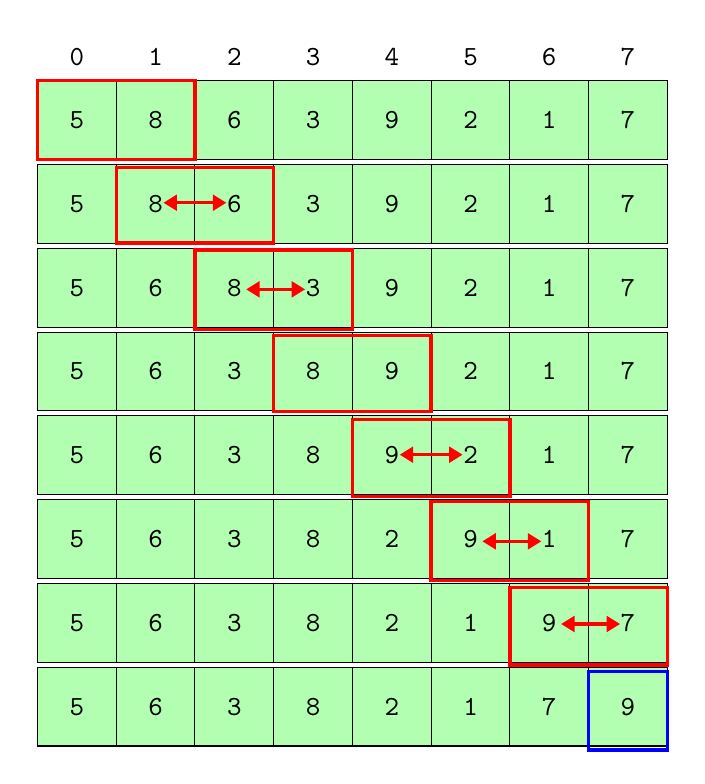
\begin{tikzpicture}[font=\ttfamily,
			array/.style={matrix of nodes,nodes={draw, minimum size=10mm, fill=green!30},column sep=-\pgflinewidth, row sep=0.5mm, nodes in empty cells,
					row 1/.style={nodes={draw=none, fill=none, minimum size=5mm}},
				}]

		\matrix[array] (array) {
			0 & 1 & 2 & 3 & 4 & 5 & 6 & 7 \\
			5 & 8 & 6 & 3 & 9 & 2 & 1 & 7 \\
			5 & 8 & 6 & 3 & 9 & 2 & 1 & 7 \\
			5 & 6 & 8 & 3 & 9 & 2 & 1 & 7 \\
			5 & 6 & 3 & 8 & 9 & 2 & 1 & 7 \\
			5 & 6 & 3 & 8 & 9 & 2 & 1 & 7 \\
			5 & 6 & 3 & 8 & 2 & 9 & 1 & 7 \\
			5 & 6 & 3 & 8 & 2 & 1 & 9 & 7 \\
			5 & 6 & 3 & 8 & 2 & 1 & 7 & 9 \\
		};

		\draw[-, very thick, red] (-4,3.95) rectangle (-2,2.95);
		\draw[-, very thick, red] (-3,2.85) rectangle (-1,1.89);
		\draw[-, very thick, red] (-2,1.8) rectangle (0,0.79);
		\draw[-, very thick, red] (-1,0.71) rectangle (1,-0.25);
		\draw[-, very thick, red] (0,-0.35) rectangle (2,-1.33);
		\draw[-, very thick, red] (1,-1.39) rectangle (3,-2.4);
		\draw[-, very thick, red] (2,-2.49) rectangle (4,-3.47);

		\draw[<->, very thick, red] (-2.4,2.4) -- (-1.6,2.4);
		\draw[<->, very thick, red] (-1.35,1.3) -- (-0.6,1.3);
		\draw[<->, very thick, red] (0.6,-0.8) -- (1.4,-0.8);
		\draw[<->, very thick, red] (1.65,-1.9) -- (2.4,-1.9);
		\draw[<->, very thick, red] (2.65,-2.95) -- (3.4,-2.95);

		\draw[-, very thick, blue] (3,-3.55) rectangle (4,-4.55);
	\end{tikzpicture}
	\caption{冒泡排序第1轮}
\end{figure}

这样一来,元素9作为数列中最大的元素,就像是汽水里的小气泡一样,浮到了最右侧。这时,冒泡排序的第1轮就结束了。数列最右侧元素9的位置可以认为是一个有序区域,有序区域目前只有1个元素。\\

接着进行第2轮排序:

\begin{figure}[H]
	\centering
	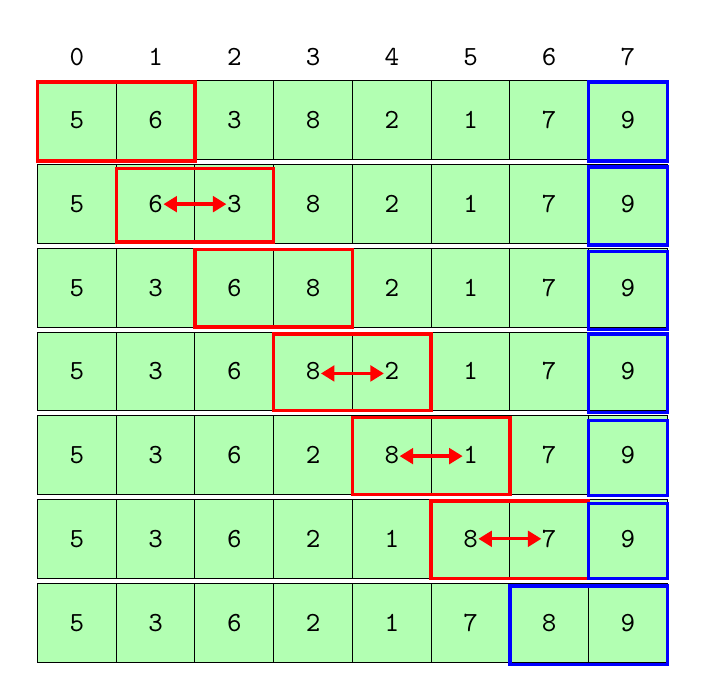
\begin{tikzpicture}[font=\ttfamily,
			array/.style={matrix of nodes,nodes={draw, minimum size=10mm, fill=green!30},column sep=-\pgflinewidth, row sep=0.5mm, nodes in empty cells,
					row 1/.style={nodes={draw=none, fill=none, minimum size=5mm}},
				}]

		\matrix[array] (array) {
			0 & 1 & 2 & 3 & 4 & 5 & 6 & 7 \\
			5 & 6 & 3 & 8 & 2 & 1 & 7 & 9 \\
			5 & 6 & 3 & 8 & 2 & 1 & 7 & 9 \\
			5 & 3 & 6 & 8 & 2 & 1 & 7 & 9 \\
			5 & 3 & 6 & 8 & 2 & 1 & 7 & 9 \\
			5 & 3 & 6 & 2 & 8 & 1 & 7 & 9 \\
			5 & 3 & 6 & 2 & 1 & 8 & 7 & 9 \\
			5 & 3 & 6 & 2 & 1 & 7 & 8 & 9 \\
		};

		\draw[-, very thick, red] (-4,3.4) rectangle (-2,2.4);
		\draw[-, very thick, red] (-3,2.3) rectangle (-1,1.37);
		\draw[-, very thick, red] (-2,1.27) rectangle (0,0.29);
		\draw[-, very thick, red] (-1,0.2) rectangle (1,-0.77);
		\draw[-, very thick, red] (0,-0.86) rectangle (2,-1.84);
		\draw[-, very thick, red] (1,-1.92) rectangle (3,-2.9);

		\draw[<->, very thick, red] (-2.4,1.85) -- (-1.6,1.85);
		\draw[<->, very thick, red] (-0.4,-0.3) -- (0.4,-0.3);
		\draw[<->, very thick, red] (0.6,-1.35) -- (1.4,-1.35);
		\draw[<->, very thick, red] (1.6,-2.4) -- (2.4,-2.4);

		\draw[-, very thick, blue] (3,3.4) rectangle (4,2.4);
		\draw[-, very thick, blue] (3,2.32) rectangle (4,1.33);
		\draw[-, very thick, blue] (3,1.25) rectangle (4,0.26);
		\draw[-, very thick, blue] (3,0.2) rectangle (4,-0.8);
		\draw[-, very thick, blue] (3,-0.9) rectangle (4,-1.85);
		\draw[-, very thick, blue] (3,-1.95) rectangle (4,-2.9);
		\draw[-, very thick, blue] (2,-3) rectangle (4,-4);
	\end{tikzpicture}
	\caption{冒泡排序第2轮}
\end{figure}

第2轮排序结束后,数列右侧的有序区有了2个元素。\\

根据相同的方法,完成剩下的排序:

\begin{figure}[H]
	\centering
	\begin{tikzpicture}[font=\ttfamily,
			array/.style={matrix of nodes,nodes={draw, minimum size=10mm, fill=green!30},column sep=-\pgflinewidth, row sep=0.5mm, nodes in empty cells,
					row 1/.style={nodes={draw=none, fill=none, minimum size=5mm}},
				}]

		\matrix[array] (array) {
			0 & 1 & 2 & 3 & 4 & 5 & 6 & 7 \\
			3 & 5 & 2 & 1 & 6 & 7 & 8 & 9 \\
			3 & 2 & 1 & 5 & 6 & 7 & 8 & 9 \\
			2 & 1 & 3 & 5 & 6 & 7 & 8 & 9 \\
			1 & 2 & 3 & 5 & 6 & 7 & 8 & 9 \\
			1 & 2 & 3 & 5 & 6 & 7 & 8 & 9 \\
		};

		\draw (-5,1.9) node{第3轮};
		\draw (-5,0.8) node{第4轮};
		\draw (-5,-0.3) node{第5轮};
		\draw (-5,-1.4) node{第6轮};
		\draw (-5,-2.4) node{第7轮};

		\draw[-, very thick, blue] (1,2.32) rectangle (4,1.33);
		\draw[-, very thick, blue] (0,1.25) rectangle (4,0.26);
		\draw[-, very thick, blue] (-1,0.2) rectangle (4,-0.8);
		\draw[-, very thick, blue] (-2,-0.9) rectangle (4,-1.85);
		\draw[-, very thick, blue] (-3,-1.95) rectangle (4,-2.9);
	\end{tikzpicture}
	\caption{冒泡排序第3 $ \sim $ 7轮}
\end{figure}

\vspace{0.5cm}

\subsection{算法分析}

冒泡排序是一种稳定排序,值相等的元素并不会打乱原本的顺序。由于该排序算法的每一轮都要遍历所有元素,总共遍历n - 1轮。

\begin{table}[H]
	\centering
	\setlength{\tabcolsep}{5mm}{
		\begin{tabular}{|c|c|c|c|}
			\hline
			\textbf{时间复杂度} & \textbf{空间复杂度} & \textbf{稳定性} & \textbf{设计思想} \\
			\hline
			$ O(n^2) $          & $ O(1) $            & 稳定            & 贪心法            \\
			\hline
		\end{tabular}
	}
	\caption{冒泡排序算法分析}
\end{table}

\mybox{冒泡排序}

\begin{lstlisting}[language=C]
void bubbleSort(int *arr, int n) {
    for(int i = 0; i < n; i++) {
        for(int j = 0; j < n-i-1; j++) {
            if(arr[j] > arr[j+1]) {
                swap(&arr[j], &arr[j+1]);
            }
        }
    }
}
\end{lstlisting}

\vspace{0.5cm}

\mybox{逆序对}\\

假设数组有n个元素,如果A[i] > A[j], i < j,那么A[i]和A[j]就被称为逆序对(inversion)。

\begin{lstlisting}[language=C]
int countInversions(int *arr, int n) {
    int cnt = 0;        // 逆序对数
    for(int i = 0; i < n-1; i++) {
        for(int j = i+1; j < n; j++) {
            if(arr[i] > arr[j]) {
                cnt++;
            }
        }
    }
    return cnt;
}
\end{lstlisting}

\vspace{0.5cm}

\subsection{冒泡排序第一次优化}

常规的冒泡排序需要进行n - 1轮循环,即使在中途数组已经有序,但是还是会继续剩下的循环。例如当数组是\{2, 1, 3, 4, 5\}时,在经过一轮排序后已经变为有序状态,再进行多余的循环就会浪费时间。\\

为了解决这个问题,可以在每一轮循环中设置一个标志。如果该轮循环中有元素发生过交换,那么就有必要进行下一轮循环。如果没有发生过交换,说明当前数组已经完成排序。\\

\mybox{冒泡排序第一次优化}

\begin{lstlisting}[language=C]
void bubbleSortOptimize1(int *arr, int n) {
    for(int i = 0; i < n - 1; i++) {
        bool hasSwapped = false;  // 标记是否发生交换
        for(int j = 0; j < n - i - 1; j++) {
            if(arr[j] > arr[j+1]) {
                swap(&arr[j], &arr[j+1]);
                hasSwapped = true;    // 发生交换
            }
        }
        // 该轮未发生交换,已经有序
        if(!hasSwapped) {
            return;
        }
    }
}
\end{lstlisting}

\vspace{0.5cm}

\subsection{冒泡排序第二次优化}

在经过一次优化后,算法还存在一个问题,例如数组\{2, 3, 1, 4, 5, 6\}在经过一轮交换后变为\{2, 1, 3, 4, 5, 6\},但是在下一轮时后面有很多次比较都是多余的,因为并没有产生交换操作。\\

为了解决这个问题,可以再设置一个标志位,用于记录当前轮所交换的最后一个元素的下标。在下一轮排序中,只需比较到该标志位即可,因此之后的元素在上一轮中没有交换过,在这一轮中也不可能交换了。\\

\mybox{冒泡排序第二次优化}

\begin{lstlisting}[language=C]
void bubbleSortOptimize2(int *arr, int n) {
    int len = n - 1;        // 内层循环执行次数
    for(int i = 0; i < n - 1; i++) {
        bool hasSwapped = false;  // 标记是否发生交换
        int last = 0;       // 标记最后一次发生交换的位置
        for(int j = 0; j < len; j++) {
            if(arr[j] > arr[j+1]) {
                swap(&arr[j], &arr[j+1]);
                hasSwapped = true;    // 发生交换
                last = j;
            }
        }
        // 该轮未发生交换,已经有序
        if(!hasSwapped) {
            return;
        }
        len = last;         // 最后一次发生交换的位置
    }
}
\end{lstlisting}

\newpage

\section{选择排序}

\subsection{选择排序(Selection Sort)}

有了冒泡排序为什么还要发明选择排序?冒泡排序有个很大的弊端,就是元素交换次数太多了。\\

想象一个场景,假设你是一名体育老师,正在指挥一群小学生按照个头从矮到高的顺序排队。采用冒泡排序的方法需要频繁交换相邻学生的位置,同学们心里恐怕会想:“这体育老师是不是有毛病啊?”\\

在程序运行的世界里,虽然计算机并不会产生什么负面情绪,但是频繁的数组元素交换意味着更多的内存读写操作,严重影响了代码运行效率。\\

有一个简单的办法,就是每一次找到个子最矮的学生,直接交换到队伍的前面。\\

例如一个有8个数字组成的无序序列,进行升序排序。

\begin{figure}[H]
	\centering
	\begin{tikzpicture}[font=\ttfamily,
			array/.style={matrix of nodes,nodes={draw, minimum size=10mm, fill=green!30},column sep=-\pgflinewidth, row sep=0.5mm, nodes in empty cells,
					row 1/.style={nodes={draw=none, fill=none, minimum size=5mm}},
				}]

		\matrix[array] (array) {
			0 & 1 & 2 & 3 & 4 & 5 & 6 & 7 \\
			5 & 8 & 6 & 3 & 9 & 2 & 1 & 7 \\
			1 & 8 & 6 & 3 & 9 & 2 & 5 & 7 \\
			1 & 2 & 6 & 3 & 9 & 8 & 5 & 7 \\
			1 & 2 & 3 & 6 & 9 & 8 & 5 & 7 \\
			1 & 2 & 3 & 5 & 9 & 8 & 6 & 7 \\
			1 & 2 & 3 & 5 & 6 & 8 & 9 & 7 \\
			1 & 2 & 3 & 5 & 6 & 7 & 9 & 8 \\
			1 & 2 & 3 & 5 & 6 & 7 & 8 & 9 \\
		};

		\draw (-5,3.4) node{原数组};
		\draw (-5,2.4) node{第1轮};
		\draw (-5,1.3) node{第2轮};
		\draw (-5,0.2) node{第3轮};
		\draw (-5,-0.9) node{第4轮};
		\draw (-5,-1.9) node{第5轮};
		\draw (-5,-3) node{第6轮};
		\draw (-5,-4) node{第7轮};

		\draw[-, very thick, blue] (-4,2.85) rectangle (-3,1.9);
		\draw[-, very thick, blue] (-4,1.8) rectangle (-2,0.8);
		\draw[-, very thick, blue] (-4,0.7) rectangle (-1,-0.25);
		\draw[-, very thick, blue] (-4,-0.35) rectangle (0,-1.3);
		\draw[-, very thick, blue] (-4,-1.4) rectangle (1,-2.4);
		\draw[-, very thick, blue] (-4,-2.5) rectangle (2,-3.45);
		\draw[-, very thick, blue] (-4,-3.55) rectangle (3,-4.5);
	\end{tikzpicture}
	\caption{选择排序}
\end{figure}

\vspace{0.5cm}

\subsection{算法分析}

算法每一轮选出最小值,再交换到左侧的时间复杂度是$ O(n) $,一共迭代n - 1轮,总的时间复杂度是$ O(n^2) $。\\

由于算法所做的是原地排序,并没有利用额外的数据结构,所以空间复杂度是$ O(1) $。

\begin{table}[H]
	\centering
	\setlength{\tabcolsep}{5mm}{
		\begin{tabular}{|c|c|c|c|}
			\hline
			\textbf{时间复杂度} & \textbf{空间复杂度} & \textbf{稳定性} & \textbf{设计思想} \\
			\hline
			$ O(n^2) $          & $ O(1) $            & 不稳定          & 减治法            \\
			\hline
		\end{tabular}
	}
	\caption{选择排序算法分析}
\end{table}

\mybox{选择排序}

\begin{lstlisting}[language=C]
void selectionSort(int *arr, int n) {
    for(int i = 0; i < n-1; i++) {
        int minIndex = i;
        for(int j = i+1; j < n; j++) {
            if(arr[j] < arr[minIndex]) {
                minIndex = j;
            }
        }
        if(i != minIndex) {
            swap(&arr[i], &arr[minIndex]);
        }
    }
}
\end{lstlisting}

\vspace{0.5cm}

\subsection{选择排序优化}

选择排序的整体思想是在一个序列当中选出一个最小的元素,和第一个元素交换,然后在剩下的找最小的,和第二个元素交换。这样最终就可以得到一个有序序列。但是为了更加高效,可以每次选择出一个最小值和一个最大值,分别放在序列的最左和最右边。\\

\mybox{选择排序优化}

\begin{lstlisting}[language=C]
void selectionSortOptimize(int *arr, int n) {
    int left = 0;
    int right = n - 1;
    while(left < right) {
        int min = left;
        int max = right;
        for(int i = left; i <= right; i++) {
            if(arr[i] < arr[min]) {
                min = i;
            }
            if(arr[i] > arr[max]) {
                max = i;
            }
        }
        swap(&arr[max], &arr[right]);
        // 考虑特殊情况,最小值在最右位置
        if(min == right) {
            min = max;
        }
        swap(&arr[min], &arr[left]);
        left++;
        right--;
    }
}
\end{lstlisting}

\newpage

\section{插入排序}

\subsection{插入排序(Insertion Sort)}

如何对扑克牌进行排序呢?例如现在手上有红桃6, 7, 9, 10这四张牌,已经处于升序排序状态。这时候抓到了一张红桃8,如何让手上的五张牌重新变成升序呢?\\

使用冒泡排序?选择排序?恐怕正常人打牌的时候都不会那么做。最自然最简单的方式,是在已经有序的四张牌中找到红桃8应该插入的位置,也就是7和9之间,把红桃8插入进去。

\begin{figure}[H]
	\centering
	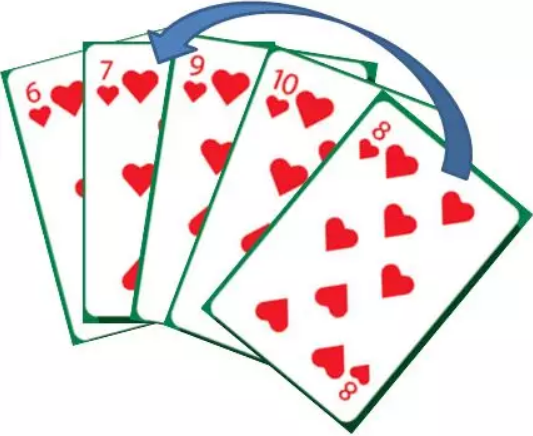
\includegraphics[scale=0.4]{img/C8/8-4/1.png}
	\caption{理牌}
\end{figure}

例如一个有8个数字组成的无序序列,进行升序排序。

\begin{figure}[H]
	\centering
	\begin{tikzpicture}[font=\ttfamily,
			array/.style={matrix of nodes,nodes={draw, minimum size=10mm, fill=green!30},column sep=-\pgflinewidth, row sep=0.5mm, nodes in empty cells,
					row 1/.style={nodes={draw=none, fill=none, minimum size=5mm}},
				}]

		\matrix[array] (array) {
			0 & 1 & 2 & 3 & 4 & 5 & 6 & 7 \\
			5 & 8 & 6 & 3 & 9 & 2 & 1 & 7 \\
			5 & 8 & 6 & 3 & 9 & 2 & 1 & 7 \\
			5 & 6 & 8 & 3 & 9 & 2 & 1 & 7 \\
			3 & 5 & 6 & 8 & 9 & 2 & 1 & 7 \\
			3 & 5 & 6 & 8 & 9 & 2 & 1 & 7 \\
			2 & 3 & 5 & 6 & 8 & 9 & 1 & 7 \\
			1 & 2 & 3 & 5 & 6 & 8 & 9 & 7 \\
			1 & 2 & 3 & 5 & 6 & 7 & 8 & 9 \\
		};

		\draw (-5,3.4) node{原数组};
		\draw (-5,2.4) node{第1轮};
		\draw (-5,1.3) node{第2轮};
		\draw (-5,0.2) node{第3轮};
		\draw (-5,-0.9) node{第4轮};
		\draw (-5,-1.9) node{第5轮};
		\draw (-5,-3) node{第6轮};
		\draw (-5,-4) node{第7轮};

		\draw[-, very thick, blue] (-4,3.9) rectangle (-3,2.95);
		\draw[-, very thick, blue] (-4,2.85) rectangle (-2,1.9);
		\draw[-, very thick, blue] (-4,1.8) rectangle (-1,0.8);
		\draw[-, very thick, blue] (-4,0.7) rectangle (0,-0.25);
		\draw[-, very thick, blue] (-4,-0.35) rectangle (1,-1.3);
		\draw[-, very thick, blue] (-4,-1.4) rectangle (2,-2.4);
		\draw[-, very thick, blue] (-4,-2.5) rectangle (3,-3.45);
		\draw[-, very thick, blue] (-4,-3.55) rectangle (4,-4.5);
	\end{tikzpicture}
	\caption{插入排序}
\end{figure}

\vspace{0.5cm}

\subsection{算法分析}

插入排序要进行n - 1轮,每一轮在最坏情况下的比较复制次数分别是1次、2次、3次、4次...一直到n - 1次,所以最坏时间复杂度是$ O(n^2) $。\\

至于空间复杂度,由于插入排序是在原地进行排序,并没有引入额外的数据结构,所以空间复杂度是$ O(1) $。

\begin{table}[H]
	\centering
	\setlength{\tabcolsep}{5mm}{
		\begin{tabular}{|c|c|c|c|}
			\hline
			\textbf{时间复杂度} & \textbf{空间复杂度} & \textbf{稳定性} & \textbf{设计思想} \\
			\hline
			$ O(n^2) $          & $ O(1) $            & 稳定            & 减治法            \\
			\hline
		\end{tabular}
	}
	\caption{插入排序算法分析}
\end{table}

\mybox{插入排序}

\begin{lstlisting}[language=C]
void insertionSort(int *arr, int n) {
    for(int i = 1; i < n; i++) {
        int temp = arr[i];
        int j = i - 1;
        while(j >= 0 && temp < arr[j]) {
            arr[j+1] = arr[j];
            j--;
        }
        arr[j+1] = temp;
    }
}
\end{lstlisting}

\vspace{0.5cm}

\subsection{折半插入排序(Binary Insertion Sort)}

折半插入排序是对插入排序的改进,其过程就是不断依次将元素插入前面已经排好序的序列中,在寻找插入点时采用了折半查找。\\

\mybox{折半插入排序}

\begin{lstlisting}[language=C]
void binaryInsertionSort(int *arr, int n) {
    for(int i = 1; i < n; i++) {
        int temp = arr[i];
        int start = 0;
        int end = i - 1;
        while(start <= end) {
            int mid = start + (end - start) / 2;
            if(arr[mid] > temp) {
                end = mid - 1;
            } else {
                start = mid + 1;
            }
        }
        int j;
        for(j = i - 1; j > end; j--) {
            arr[j+1] = arr[j];
        }
        arr[j+1] = temp;
    }
}
\end{lstlisting}

\newpage

\section{鸡尾酒排序}

\subsection{鸡尾酒排序(Cocktail Sort)}

对一个无序数组\{2, 3, 4, 5, 6, 7, 8, 1\}进行升序排序,如果按照冒泡排序,步骤如下:

\begin{figure}[H]
	\centering
	\begin{tikzpicture}[font=\ttfamily,
			array/.style={matrix of nodes,nodes={draw, minimum size=10mm, fill=green!30},column sep=-\pgflinewidth, row sep=0.5mm, nodes in empty cells,
					row 1/.style={nodes={draw=none, fill=none, minimum size=5mm}},
				}]

		\matrix[array] (array) {
			0 & 1 & 2 & 3 & 4 & 5 & 6 & 7 \\
			2 & 3 & 4 & 5 & 6 & 7 & 1 & 8 \\
			2 & 3 & 4 & 5 & 6 & 7 & 1 & 8 \\
			2 & 3 & 4 & 5 & 6 & 1 & 7 & 8 \\
			2 & 3 & 4 & 5 & 1 & 6 & 7 & 8 \\
			2 & 3 & 4 & 1 & 5 & 6 & 7 & 8 \\
			2 & 3 & 1 & 4 & 5 & 6 & 7 & 8 \\
			2 & 1 & 3 & 4 & 5 & 6 & 7 & 8 \\
			1 & 2 & 3 & 4 & 5 & 6 & 7 & 8 \\
		};

		\draw (-5,3.4) node{原数组};
		\draw (-5,2.4) node{第1轮};
		\draw (-5,1.3) node{第2轮};
		\draw (-5,0.2) node{第3轮};
		\draw (-5,-0.9) node{第4轮};
		\draw (-5,-1.9) node{第5轮};
		\draw (-5,-3) node{第6轮};
		\draw (-5,-4) node{第7轮};

		\draw[-, very thick, blue] (3,2.85) rectangle (4,1.9);
		\draw[-, very thick, blue] (2,1.8) rectangle (4,0.8);
		\draw[-, very thick, blue] (1,0.7) rectangle (4,-0.25);
		\draw[-, very thick, blue] (0,-0.35) rectangle (4,-1.3);
		\draw[-, very thick, blue] (-1,-1.4) rectangle (4,-2.4);
		\draw[-, very thick, blue] (-2,-2.5) rectangle (4,-3.45);
		\draw[-, very thick, blue] (-3,-3.55) rectangle (4,-4.5);
	\end{tikzpicture}
	\caption{冒泡排序}
\end{figure}

从2到8已经是有序了,只有元素1的位置不对,却还要进行7轮排序,这也太憋屈了吧!\\

鸡尾酒排序正是用于解决这种问题的。鸡尾酒排序又叫快乐小时排序,它基于冒泡排序做了一点小小的优化。\\

鸡尾酒排序的第一轮与冒泡排序相同,从左向右比较和交换。

\begin{figure}[H]
	\centering
	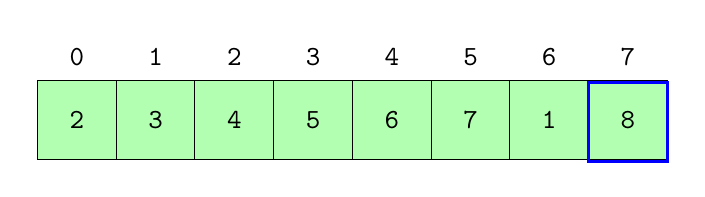
\begin{tikzpicture}[font=\ttfamily,
			array/.style={matrix of nodes,nodes={draw, minimum size=10mm, fill=green!30},column sep=-\pgflinewidth, row sep=0.5mm, nodes in empty cells,
					row 1/.style={nodes={draw=none, fill=none, minimum size=5mm}},
				}]

		\matrix[array] (array) {
			0 & 1 & 2 & 3 & 4 & 5 & 6 & 7 \\
			2 & 3 & 4 & 5 & 6 & 7 & 1 & 8 \\
		};

		\draw[-, very thick, blue] (3,0.2) rectangle (4,-0.8);
	\end{tikzpicture}
	\caption{鸡尾酒排序第1轮}
\end{figure}

第二轮开始不一样了,反过来向右向左比较和交换。

\begin{figure}[H]
	\centering
	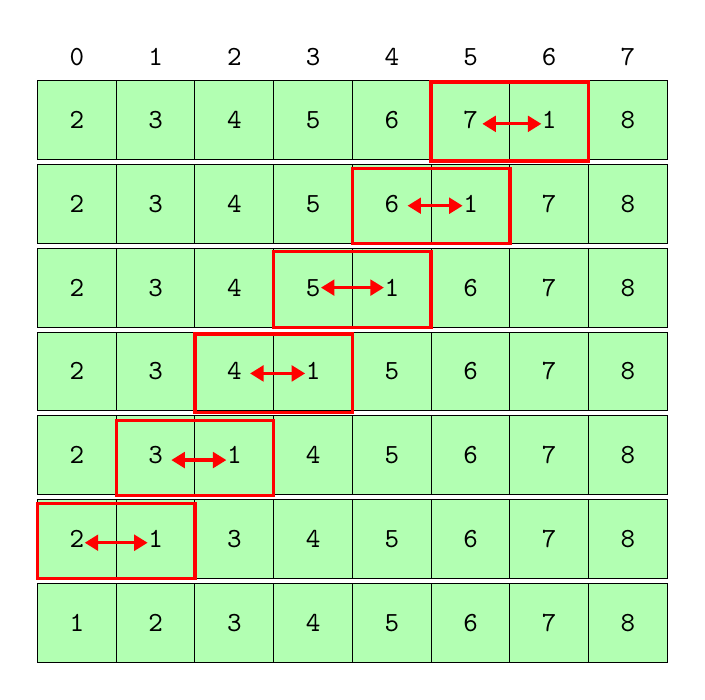
\begin{tikzpicture}[font=\ttfamily,
			array/.style={matrix of nodes,nodes={draw, minimum size=10mm, fill=green!30},column sep=-\pgflinewidth, row sep=0.5mm, nodes in empty cells,
					row 1/.style={nodes={draw=none, fill=none, minimum size=5mm}},
				}]

		\matrix[array] (array) {
			0 & 1 & 2 & 3 & 4 & 5 & 6 & 7 \\
			2 & 3 & 4 & 5 & 6 & 7 & 1 & 8 \\
			2 & 3 & 4 & 5 & 6 & 1 & 7 & 8 \\
			2 & 3 & 4 & 5 & 1 & 6 & 7 & 8 \\
			2 & 3 & 4 & 1 & 5 & 6 & 7 & 8 \\
			2 & 3 & 1 & 4 & 5 & 6 & 7 & 8 \\
			2 & 1 & 3 & 4 & 5 & 6 & 7 & 8 \\
			1 & 2 & 3 & 4 & 5 & 6 & 7 & 8 \\
		};

		\draw[-, very thick, red] (1,3.4) rectangle (3,2.4);
		\draw[-, very thick, red] (0,2.3) rectangle (2,1.35);
		\draw[-, very thick, red] (-1,1.25) rectangle (1,0.28);
		\draw[-, very thick, red] (-2,0.2) rectangle (0,-0.8);
		\draw[-, very thick, red] (-3,-0.9) rectangle (-1,-1.85);
		\draw[-, very thick, red] (-4,-1.95) rectangle (-2,-2.9);

		\draw[<->, very thick, red] (1.65,2.87) -- (2.4,2.87);
		\draw[<->, very thick, red] (0.7,1.83) -- (1.4,1.83);
		\draw[<->, very thick, red] (-0.4,0.79) -- (0.4,0.79);
		\draw[<->, very thick, red] (-1.3,-0.3) -- (-0.6,-0.3);
		\draw[<->, very thick, red] (-2.3,-1.4) -- (-1.6,-1.4);
		\draw[<->, very thick, red] (-3.4,-2.45) -- (-2.6,-2.45);
	\end{tikzpicture}
	\caption{鸡尾酒排序第2轮}
\end{figure}

第二轮结束后,此时虽然已经有序,但是算法并没有结束。\\

第三轮再次从左向右比较和交换,在此过程中,没有元素发生交换,证明已经有序,排序结束。\\

鸡尾酒排序的过程就像钟摆一样,左右来回比较和交换。本来冒泡要用8轮排序的场景,鸡尾酒用3轮就解决了。\\

鸡尾酒排序的优点是能够在大部分元素已经有序的情况下,减少排序的回合数;而缺点也很明显,就是代码量几乎扩大了一倍。\\

\mybox{鸡尾酒排序}

\begin{lstlisting}[language=C]
void cocktailSort1(int *arr, int n) {
    for(int i = 0; i < n / 2; i++) {
        // 从左向右
        bool isSorted = true;   // 标记当前轮是否有序
        for(int j = i; j < n - i - 1; j++) {
            if(arr[j] > arr[j+1]) {
                swap(&arr[j], &arr[j+1]);
                isSorted = false;   // 发生交换
            }
        }
        if(isSorted) {
            break;
        }

        // 从右向左
        isSorted = true;
        for(int j = n - i - 1; j > i; j--) {
            if(arr[j] < arr[j-1]) {
                swap(&arr[j], &arr[j-1]);
                isSorted = false;
            }
        }
        if(isSorted) {
            break;
        }
    }
}
\end{lstlisting}

\vspace{0.5cm}

\subsection{鸡尾酒排序优化}

类似冒泡排序的优化方法,鸡尾酒排序也可以记录每一轮排序后最后一次元素交换的位置。但是对于双向的鸡尾酒排序而言,需要设置两个边界值。\\

\mybox{鸡尾酒排序优化}

\begin{lstlisting}[language=C]
void cocktailSort2(int *arr, int n) {
    int lastLeft = 0;           // 左侧最后一次交换位置
    int lastRight = 0;          // 右侧最后一次交换位置
    int leftBorder = 0;         // 无序区左边界
    int rightBorder = n - 1;    // 无序区右边界

    for(int i = 0; i < n / 2; i++) {
        // 从左向右
        bool isSorted = true;   // 标记当前轮是否有序
        for(int j = leftBorder; j < rightBorder; j++) {
            if(arr[j] > arr[j+1]) {
                swap(&arr[j], &arr[j+1]);
                isSorted = false;   // 发生交换
                lastRight = j;
            }
        }
        if(isSorted) {
            break;
        }
        rightBorder = lastRight;

        // 从右向左
        isSorted = true;
        for(int j = n - i - 1; j > i; j--) {
            if(arr[j] < arr[j-1]) {
                swap(&arr[j], &arr[j-1]);
                isSorted = false;
                lastLeft = j;
            }
        }
        if(isSorted) {
            break;
        }
        leftBorder = lastLeft;
    }
}
\end{lstlisting}

\newpage

\section{归并排序}

\subsection{归并排序(Merge Sort)}

归并排序算法采用分治法:

\begin{enumerate}
	\item 分解:将序列每次折半划分。
	\item 合并:将划分后的序列两两按序合并。
\end{enumerate}

\begin{figure}[H]
	\centering
	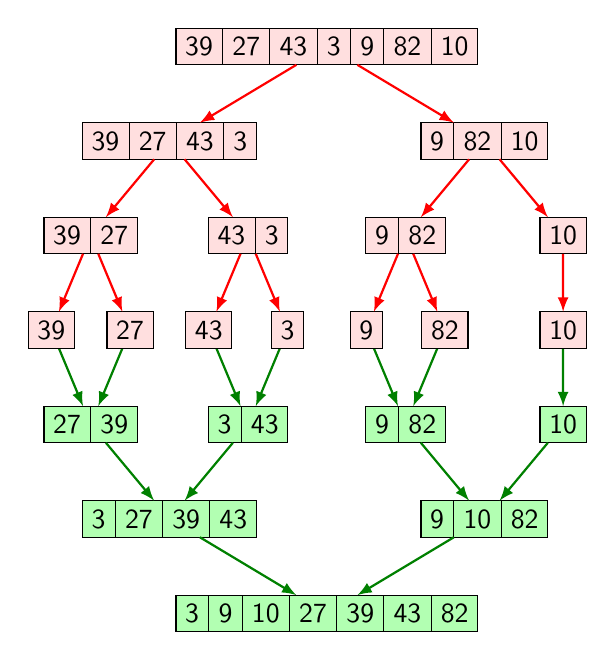
\begin{tikzpicture}[level distance=1.2cm,
			level 1/.style={sibling distance=4cm},
			level 2/.style={sibling distance=2cm},
			level 3/.style={sibling distance=1cm},
			edgedown/.style={edge from parent/.style={draw=red,thick,-latex}},
			edgeup/.style={edge from parent/.style={draw=green!50!black,thick,latex-}}
		]

		\node[gblock=7,yshift=-7.2cm] (A') {3 \nodepart{two} 9 \nodepart{three} 10 \nodepart{four} 27 \nodepart{five} 39 \nodepart{six}43 \nodepart{seven}82}
		[grow=up,edgeup]
		child {node[gblock=3] (B2') {9 \nodepart{two} 10 \nodepart{three} 82}
				child {node[gblock=1] (C4') {10}
						child {node[gblock=1] (D7') {10}}
					}
				child {node[gblock=2] (C2') {9 \nodepart{two} 82}
						child {node[gblock=1] (D3') {82}}
						child {node[gblock=1] (D4') {9}}
					}
			}
		child {node[gblock=4] (B1') {3 \nodepart{two} 27 \nodepart{three} 39 \nodepart{four} 43}
				child {node[gblock=2] (C3') {3 \nodepart{two} 43}
						child {node[gblock=1] (D5') {3}}
						child {node[gblock=1] (D6') {43}}
					}
				child {node[gblock=2] (C1') {27 \nodepart{two} 39}
						child {node[gblock=1] (D1') {27}}
						child {node[gblock=1] (D2') {39}}
					}
			};

		\node[block=7] (A) {39 \nodepart{two} 27 \nodepart{three} 43 \nodepart{four} 3 \nodepart{five} 9 \nodepart{six}82 \nodepart{seven}10}
		[grow=down,edgedown]
		child {node[block=4] (B1) {39 \nodepart{two} 27 \nodepart{three} 43 \nodepart{four} 3}
				child {node[block=2] (C1) {39 \nodepart{two} 27}
						child {node[block=1] (D1) {39}}
						child {node[block=1] (D2) {27}}
					}
				child {node[block=2] (C2) {43 \nodepart{two} 3}
						child {node[block=1] (D3) {43}}
						child {node[block=1] (D4) {3}}
					}
			}
		child {node[block=3] (B2) {9 \nodepart{two} 82 \nodepart{three} 10}
				child {node[block=2] (C3) {9 \nodepart{two} 82}
						child {node[block=1] (D5) {9}}
						child {node[block=1] (D6) {82}}
					}
				child {node[block=1] (C4) {10}
						child {node[block=1] (D7) {10}}
					}
			};
	\end{tikzpicture}
	\caption{归并排序}
\end{figure}

\vspace{0.5cm}

\subsection{算法分析}

归并排序每次将数组折半对分,一共分了$ logn $次,每一层进行合并操作的运算量是n,所以时间复杂度为$ O(nlogn) $。归并排序的速度仅次于快速排序。\\

\begin{table}[H]
	\centering
	\setlength{\tabcolsep}{5mm}{
		\begin{tabular}{|c|c|c|c|}
			\hline
			\textbf{时间复杂度} & \textbf{空间复杂度} & \textbf{稳定性} & \textbf{设计思想} \\
			\hline
			$ O(nlogn) $        & $ O(n) $            & 稳定            & 分治法            \\
			\hline
		\end{tabular}
	}
	\caption{归并排序算法分析}
\end{table}

\mybox{归并排序}

\begin{lstlisting}[language=C]
void merge(int *arr, int start, int mid, int end, int *temp) {
    int i = start;
    int j = mid + 1;
    int k = 0;

    while(i <= mid && j <= end) {
        if(arr[i] <= arr[j]) {
            temp[k++] = arr[i++];
        } else {
            temp[k++] = arr[j++];
        }
    }

    while(i <= mid) {
        temp[k++] = arr[i++];
    }
    while(j <= end) {
        temp[k++] = arr[j++];
    }

    for(int i = 0; i < k; i++) {
        arr[start+i] = temp[i];
    }
}

void mergeSort(int *arr, int start, int end, int *temp) {
    if(start < end) {
        int mid = start + (end - start) / 2;
        mergeSort(arr, start, mid, temp);
        mergeSort(arr, mid+1, end, temp);
        merge(arr, start, mid, end, temp);
    }
}
\end{lstlisting}

\newpage

\section{快速排序}

\subsection{快速排序(Quick Sort)}

快速排序是很重要的算法,与傅里叶变换等算法并称二十世纪十大算法。\\

快速排序之所以快,是因为它使用了分治法。快速排序在每一轮挑选一个基准(pivot)元素,并让其它比它小的元素移动到数列一边,比它大的元素移动到数列的另一边,从而把数列拆解成了两个部分。\\

选择基准元素最简单的方式是选择数列的第一个元素。这种选择在绝大多数情况下是没有问题的,但是如果对一个原本逆序的数列进行升序排序,整个数列并没有被分成一半,每一轮仅仅确定了基准元素的位置。这种情况下数列第一个元素要么是最小值,要么是最大值,根本无法发挥分治法的优势。在这种极端情况下,快速排序需要进行n轮,时间复杂度退化成了$ O(n^2) $。

如何避免这种极端情况呢?可以不选择数列的第一个元素,而是随机选择一个元素作为基准元素。这样一来,即使是在数列完全逆序的情况下,也可以有效地将数列分成两部分。当然,即使是随机选择,每一次也有极小的几率选到数列的最大值或最小值,同样会对分治造成一定影响。\\

确定了基准值后,如何实现将小于基准的元素都移动到基准值一边,大于基准值的都移动到另一边呢?\\

例如一个有8个数字组成的无序序列,进行升序排序。选定基准元素pivot,设置两个指针left和right,指向数列的最左和最右两个元素。

\begin{figure}[H]
	\centering
	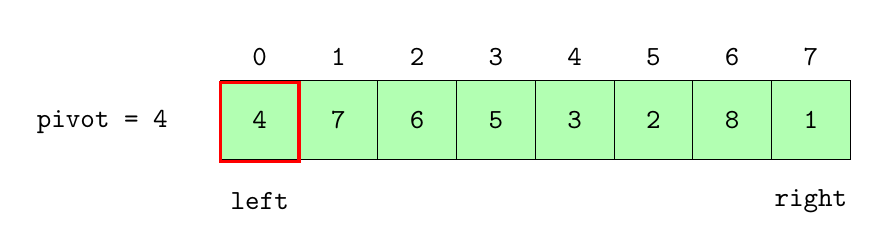
\begin{tikzpicture}[font=\ttfamily,
			array/.style={matrix of nodes,nodes={draw, minimum size=10mm, fill=green!30},column sep=-\pgflinewidth, row sep=0.5mm, nodes in empty cells,
					row 1/.style={nodes={draw=none, fill=none, minimum size=5mm}},
				}]

		\matrix[array] (array) {
			0 & 1 & 2 & 3 & 4 & 5 & 6 & 7 \\
			4 & 7 & 6 & 5 & 3 & 2 & 8 & 1 \\
		};

		\draw (-5.5,-0.3) node{pivot = 4};
		\draw[-, very thick, red] (-4,0.2) rectangle (-3,-0.8);
		\draw (-3.5,-1.3) node{left};
		\draw (3.5,-1.3) node{right};
	\end{tikzpicture}
\end{figure}

从right指针开始,把指针所指向的元素和基准元素做比较。如果比pivot大,则right指针向左移动;如果比pivot小,则把right所指向的元素填入left指针所指向的位置,同时left向右移动一位。

\begin{figure}[H]
	\centering
	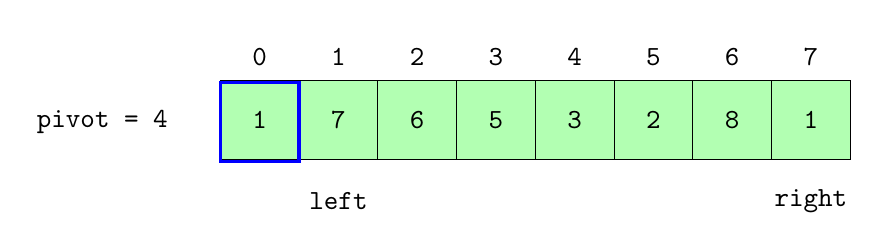
\begin{tikzpicture}[font=\ttfamily,
			array/.style={matrix of nodes,nodes={draw, minimum size=10mm, fill=green!30},column sep=-\pgflinewidth, row sep=0.5mm, nodes in empty cells,
					row 1/.style={nodes={draw=none, fill=none, minimum size=5mm}},
				}]

		\matrix[array] (array) {
			0 & 1 & 2 & 3 & 4 & 5 & 6 & 7 \\
			1 & 7 & 6 & 5 & 3 & 2 & 8 & 1 \\
		};

		\draw (-5.5,-0.3) node{pivot = 4};
		\draw[-, very thick, blue] (-4,0.2) rectangle (-3,-0.8);
		\draw (-2.5,-1.3) node{left};
		\draw (3.5,-1.3) node{right};
	\end{tikzpicture}
\end{figure}

接着,切换到left指针进行比较,把指针所指向的元素和基准元素做比较。如果小于pivot,则left指针向右移动;如果大于pivot,则把left所指向的元素填入right指针所指向的位置,同时right向左移动一位。

\begin{figure}[H]
	\centering
	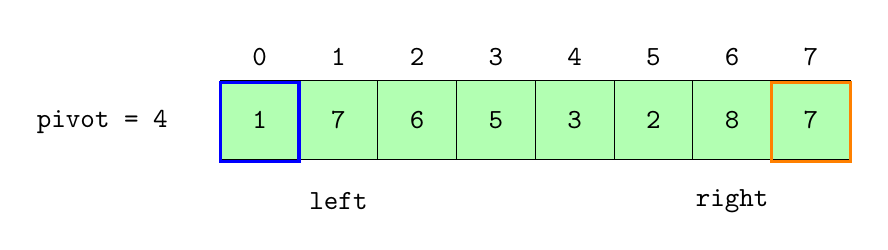
\begin{tikzpicture}[font=\ttfamily,
			array/.style={matrix of nodes,nodes={draw, minimum size=10mm, fill=green!30},column sep=-\pgflinewidth, row sep=0.5mm, nodes in empty cells,
					row 1/.style={nodes={draw=none, fill=none, minimum size=5mm}},
				}]

		\matrix[array] (array) {
			0 & 1 & 2 & 3 & 4 & 5 & 6 & 7 \\
			1 & 7 & 6 & 5 & 3 & 2 & 8 & 7 \\
		};

		\draw (-5.5,-0.3) node{pivot = 4};
		\draw[-, very thick, blue] (-4,0.2) rectangle (-3,-0.8);
		\draw[-, very thick, orange] (3,0.2) rectangle (4,-0.8);
		\draw (-2.5,-1.3) node{left};
		\draw (2.5,-1.3) node{right};
	\end{tikzpicture}
\end{figure}

重复之前的步骤继续排序:

\begin{figure}[H]
	\centering
	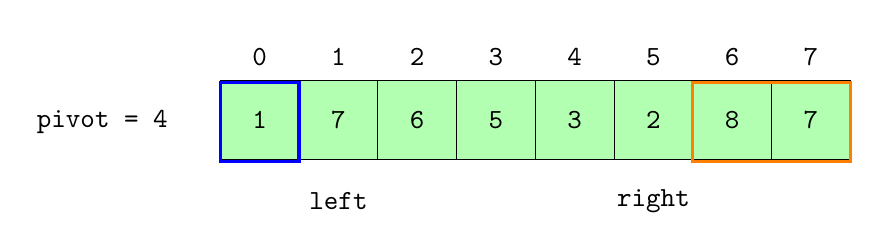
\begin{tikzpicture}[font=\ttfamily,
			array/.style={matrix of nodes,nodes={draw, minimum size=10mm, fill=green!30},column sep=-\pgflinewidth, row sep=0.5mm, nodes in empty cells,
					row 1/.style={nodes={draw=none, fill=none, minimum size=5mm}},
				}]

		\matrix[array] (array) {
			0 & 1 & 2 & 3 & 4 & 5 & 6 & 7 \\
			1 & 7 & 6 & 5 & 3 & 2 & 8 & 7 \\
		};

		\draw (-5.5,-0.3) node{pivot = 4};
		\draw[-, very thick, blue] (-4,0.2) rectangle (-3,-0.8);
		\draw[-, very thick, orange] (2,0.2) rectangle (4,-0.8);
		\draw (-2.5,-1.3) node{left};
		\draw (1.5,-1.3) node{right};
	\end{tikzpicture}

	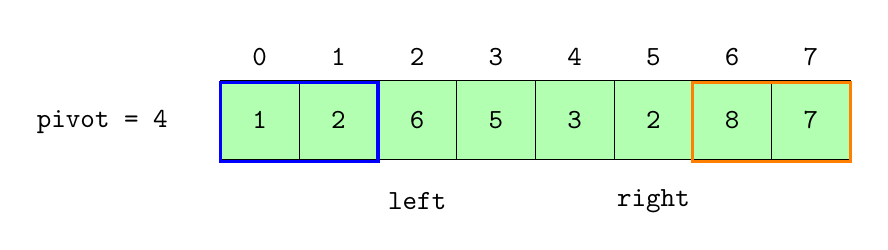
\begin{tikzpicture}[font=\ttfamily,
			array/.style={matrix of nodes,nodes={draw, minimum size=10mm, fill=green!30},column sep=-\pgflinewidth, row sep=0.5mm, nodes in empty cells,
					row 1/.style={nodes={draw=none, fill=none, minimum size=5mm}},
				}]

		\matrix[array] (array) {
			0 & 1 & 2 & 3 & 4 & 5 & 6 & 7 \\
			1 & 2 & 6 & 5 & 3 & 2 & 8 & 7 \\
		};

		\draw (-5.5,-0.3) node{pivot = 4};
		\draw[-, very thick, blue] (-4,0.2) rectangle (-2,-0.8);
		\draw[-, very thick, orange] (2,0.2) rectangle (4,-0.8);
		\draw (-1.5,-1.3) node{left};
		\draw (1.5,-1.3) node{right};
	\end{tikzpicture}

	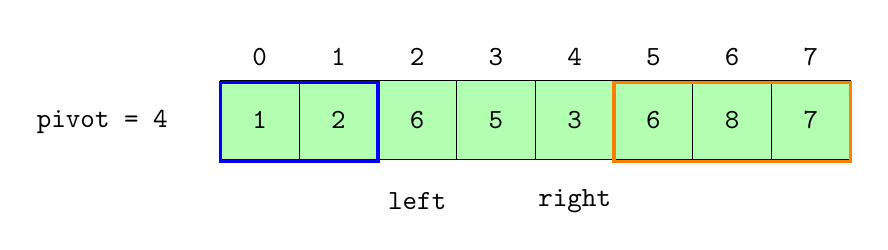
\begin{tikzpicture}[font=\ttfamily,
			array/.style={matrix of nodes,nodes={draw, minimum size=10mm, fill=green!30},column sep=-\pgflinewidth, row sep=0.5mm, nodes in empty cells,
					row 1/.style={nodes={draw=none, fill=none, minimum size=5mm}},
				}]

		\matrix[array] (array) {
			0 & 1 & 2 & 3 & 4 & 5 & 6 & 7 \\
			1 & 2 & 6 & 5 & 3 & 6 & 8 & 7 \\
		};

		\draw (-5.5,-0.3) node{pivot = 4};
		\draw[-, very thick, blue] (-4,0.2) rectangle (-2,-0.8);
		\draw[-, very thick, orange] (1,0.2) rectangle (4,-0.8);
		\draw (-1.5,-1.3) node{left};
		\draw (0.5,-1.3) node{right};
	\end{tikzpicture}

	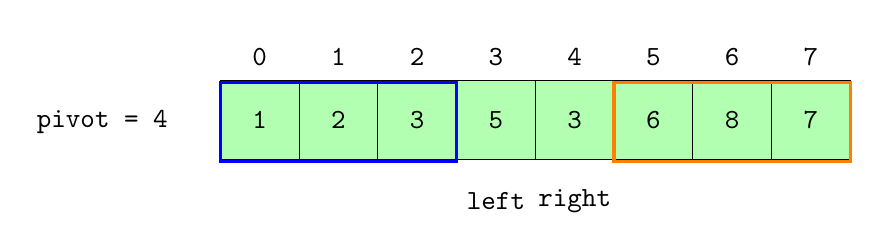
\begin{tikzpicture}[font=\ttfamily,
			array/.style={matrix of nodes,nodes={draw, minimum size=10mm, fill=green!30},column sep=-\pgflinewidth, row sep=0.5mm, nodes in empty cells,
					row 1/.style={nodes={draw=none, fill=none, minimum size=5mm}},
				}]

		\matrix[array] (array) {
			0 & 1 & 2 & 3 & 4 & 5 & 6 & 7 \\
			1 & 2 & 3 & 5 & 3 & 6 & 8 & 7 \\
		};

		\draw (-5.5,-0.3) node{pivot = 4};
		\draw[-, very thick, blue] (-4,0.2) rectangle (-1,-0.8);
		\draw[-, very thick, orange] (1,0.2) rectangle (4,-0.8);
		\draw (-0.5,-1.3) node{left};
		\draw (0.5,-1.3) node{right};
	\end{tikzpicture}

	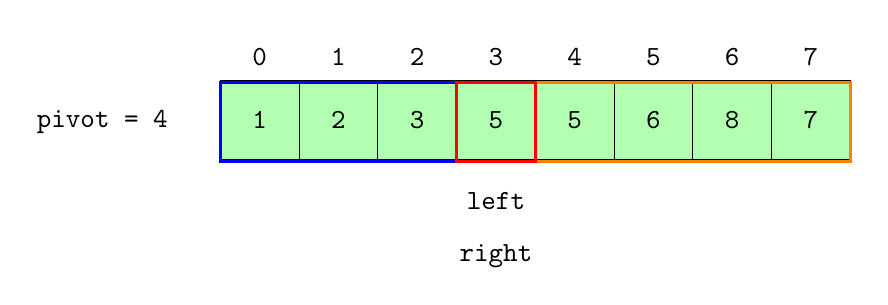
\begin{tikzpicture}[font=\ttfamily,
			array/.style={matrix of nodes,nodes={draw, minimum size=10mm, fill=green!30},column sep=-\pgflinewidth, row sep=0.5mm, nodes in empty cells,
					row 1/.style={nodes={draw=none, fill=none, minimum size=5mm}},
				}]

		\matrix[array] (array) {
			0 & 1 & 2 & 3 & 4 & 5 & 6 & 7 \\
			1 & 2 & 3 & 5 & 5 & 6 & 8 & 7 \\
		};

		\draw (-5.5,-0.3) node{pivot = 4};
		\draw[-, very thick, blue] (-4,0.2) rectangle (-1,-0.8);
		\draw[-, very thick, orange] (0,0.2) rectangle (4,-0.8);
		\draw[-, very thick, red] (-1,0.2) rectangle (0,-0.8);
		\draw (-0.5,-1.3) node{left};
		\draw (-0.5,-2) node{right};
	\end{tikzpicture}
\end{figure}

当left和right指针重合在同一位置的时候,把之前的pivot元素的值填入该重合的位置。此时数列左边的元素都小于基准元素,数列右边的元素都大于基准元素。\\

\subsection{算法分析}

分治法的思想下,原数列在每一轮被拆分成两部分,每一部分在下一轮又被拆分成两部分,直到不可再分为止。这样平均情况下需要$ logn $轮,因此快速排序算法的平均时间复杂度是$ O(nlogn) $。

\begin{table}[H]
	\centering
	\setlength{\tabcolsep}{5mm}{
		\begin{tabular}{|c|c|c|c|}
			\hline
			\textbf{时间复杂度}      & \textbf{空间复杂度}   & \textbf{稳定性} & \textbf{设计思想} \\
			\hline
			$ O(nlogn) \sim O(n^2) $ & $ O(logn) \sim O(n) $ & 不稳定          & 分治法            \\
			\hline
		\end{tabular}
	}
	\caption{快速排序算法分析}
\end{table}

\mybox{快速排序}

\begin{lstlisting}[language=C]
void quickSort(int *arr, int start, int end) {
    if(start < end) {
        int i = start;
        int j = end;
        int pivot = arr[start];

        while(i < j) {
            while(i < j && arr[j] > pivot) {
                j--;
            }
            if(i < j) {
                arr[i] = arr[j];
                i++;
            }
            while(i < j && arr[i] < pivot) {
                i++;
            }
            if(i < j) {
                arr[j] = arr[i];
                j--;
            }
        }
        arr[i] = pivot;
        quickSort(arr, start, i-1);
        quickSort(arr, i+1, end);
    } 
}
\end{lstlisting}

\newpage

\section{计数排序}

\subsection{计数排序(Counting Sort)}

基于比较的排序算法的最优下界为$ \Omega(nlogn) $。计数排序是一种不基于比较的排序算法,而是利用数组下标来确定元素的正确位置。\\

遍历数列,将每一个整数按照其值对号入座,对应数组下标的元素加1。数组的每一个下标位置的值,代表了数列中对应整数出现的次数。有了这个统计结果,直接遍历数组,输出数组元素的下标值,元素的值是多少就输出多少次。\\

从功能角度,这个算法可以实现整数的排序,但是也存在一些问题。如果只以最大值来决定统计数组的长度并不严谨,例如数列\{95, 94, 91, 98, 99, 90, 99, 93, 91, 92\},这个数列的最大值是99,但最小值是90。如果创建长度为100的数组,前面的从0到89的空间位置都浪费了。\\

因此,不应再以数列的max + 1作为统计数组的长度,而是以数列max - min + 1作为统计数组的长度。同时,数列的最小值作为一个偏移量,用于统计数组的对号入座。\\

计数排序适用于一定范围的整数排序,在取值范围不是很大的情况下,它的性能甚至快过那些$ O(nlogn) $的排序算法。\\

\mybox{计数排序}

\begin{lstlisting}[language=C]
void countingSort(int *arr, int n) {
    int max = arr[0];
    int min = arr[0];
    for(int i = 1; i < n; i++) {
        if(arr[i] > max) {
            max = arr[i];
        }
        if(arr[i] < min) {
            min = arr[i];
        }
    }
    
    int range = max - min + 1;
    int table[range];
    memset(table, 0, sizeof(table));

    for(int i = 0; i < n; i++) {
        table[arr[i] - min]++;
    }

    int cnt = 0;
    for(int i = 0; i < range; i++) {
        while(table[i]--) {
            arr[cnt++] = i + min;
        }
    }
}
\end{lstlisting}

\newpage

\section{桶排序}

\subsection{桶排序(Bucket Sort)}

桶排序是计数排序的扩展版本。计数排序可以看成每个桶只存储相同元素,而桶排序每个桶存储一定范围的元素。\\

每一个桶代表一个区间范围,里面可以承载一个或多个元素。通过划分多个范围相同的区间,将每个子区间自排序,最后合并。桶排序需要尽量保证元素分散均匀,否则当所有数据集中在同一个桶中时,桶排序失效。\\

例如一个待排序的序列:

\begin{figure}[H]
	\centering
	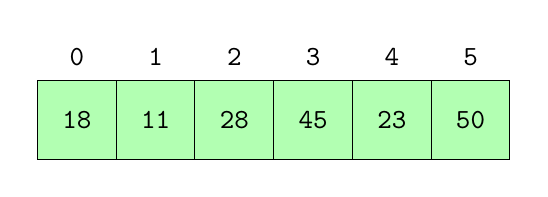
\begin{tikzpicture}[font=\ttfamily,
			array/.style={matrix of nodes,nodes={draw, minimum size=10mm, fill=green!30},column sep=-\pgflinewidth, row sep=0.5mm, nodes in empty cells,
					row 1/.style={nodes={draw=none, fill=none, minimum size=5mm}},
				}]

		\matrix[array] (array) {
			0  & 1  & 2  & 3  & 4  & 5  \\
			18 & 11 & 28 & 45 & 23 & 50 \\
		};
	\end{tikzpicture}
\end{figure}

确定桶的个数与每个桶的取值范围,遍历待排序序列,将元素放入对应的桶中:

\begin{figure}[H]
	\centering
	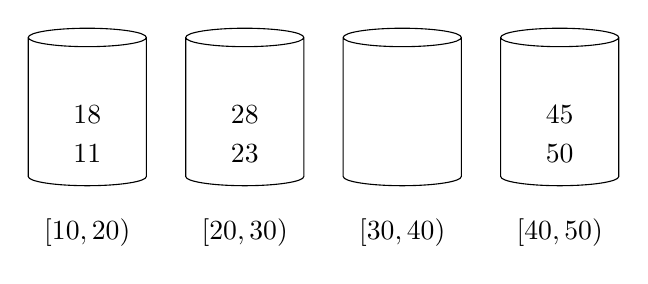
\begin{tikzpicture}
		\node (a) [cylinder, xshift=0cm, shape border rotate=90, draw, minimum height=20mm, minimum width=15mm] {};
		\node (b) [cylinder, xshift=2cm, shape border rotate=90, draw, minimum height=20mm, minimum width=15mm] {};
		\node (c) [cylinder, xshift=4cm, shape border rotate=90, draw, minimum height=20mm, minimum width=15mm] {};
		\node (d) [cylinder, xshift=6cm, shape border rotate=90, draw, minimum height=20mm, minimum width=15mm] {};

		\draw (0,-1.5) node{$ [10, 20) $};
			\draw (2,-1.5) node{$ [20, 30) $};
		\draw (4,-1.5) node{$ [30, 40) $};
			\draw (6,-1.5) node{$ [40, 50) $};

		\draw (0,0) node{18};
		\draw (0,-0.5) node{11};
		\draw (2,0) node{28};
		\draw (2,-0.5) node{23};
		\draw (6,0) node{45};
		\draw (6,-0.5) node{50};
	\end{tikzpicture}
\end{figure}

分别对每个桶中的元素进行排序:

\begin{figure}[H]
	\centering
	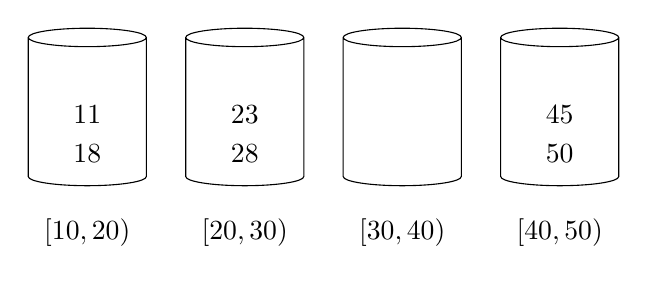
\begin{tikzpicture}
		\node (a) [cylinder, xshift=0cm, shape border rotate=90, draw, minimum height=20mm, minimum width=15mm] {};
		\node (b) [cylinder, xshift=2cm, shape border rotate=90, draw, minimum height=20mm, minimum width=15mm] {};
		\node (c) [cylinder, xshift=4cm, shape border rotate=90, draw, minimum height=20mm, minimum width=15mm] {};
		\node (d) [cylinder, xshift=6cm, shape border rotate=90, draw, minimum height=20mm, minimum width=15mm] {};

		\draw (0,-1.5) node{$ [10, 20) $};
			\draw (2,-1.5) node{$ [20, 30) $};
		\draw (4,-1.5) node{$ [30, 40) $};
			\draw (6,-1.5) node{$ [40, 50) $};

		\draw (0,0) node{11};
		\draw (0,-0.5) node{18};
		\draw (2,0) node{23};
		\draw (2,-0.5) node{28};
		\draw (6,0) node{45};
		\draw (6,-0.5) node{50};
	\end{tikzpicture}
\end{figure}

将桶中的元素按顺序赋值到原始数组中:

\begin{figure}[H]
	\centering
	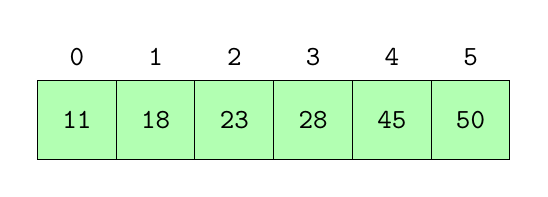
\begin{tikzpicture}[font=\ttfamily,
			array/.style={matrix of nodes,nodes={draw, minimum size=10mm, fill=green!30},column sep=-\pgflinewidth, row sep=0.5mm, nodes in empty cells,
					row 1/.style={nodes={draw=none, fill=none, minimum size=5mm}},
				}]

		\matrix[array] (array) {
			0  & 1  & 2  & 3  & 4  & 5  \\
			11 & 18 & 23 & 28 & 45 & 50 \\
		};
	\end{tikzpicture}
\end{figure}

创建桶的数量取决于数据的区间范围,一般创建桶的数量等于待排序的元素数量,每个桶的区间跨度为:

$$
	max - min \over buckets - 1
$$

\vspace{0.5cm}

\mybox{桶排序}

\begin{lstlisting}[language=Java]
public static void bucketSort(int[] arr) {
        int max = arr[0];
        int min = arr[0];
        for(int i = 1; i < arr.length; i++) {
            if(arr[i] > max) {
                max = arr[i];
            }
            if(arr[i] < min) {
                min = arr[i];
            }
        }
        int diff = max - min;

        // 创建桶
        int bucketNum = arr.length;
        List<LinkedList<Integer>> buckets 
            = new ArrayList<>(bucketNum);
        for(int i = 0; i < bucketNum; i++) {
            buckets.add(new LinkedList<>());
        }

        // 遍历数组,把元素放入对应桶中
        for(int i = 0; i < arr.length; i++) {
            // 计算当前元素所放置的桶号
            int num = (arr[i]-min) / (diff / (bucketNum-1));
            buckets.get(num).add(arr[i]);
        }

        // 桶内排序
        for(int i = 0; i < bucketNum; i++) {
            Collections.sort(buckets.get(i));
        }

        // 取出元素
        int cnt = 0;
        for(LinkedList<Integer> list : buckets) {
            for(int data : list) {
                arr[cnt++] = data;
            }
        }
    }
\end{lstlisting}

\newpage

\section{基数排序}

\subsection{基数排序(Radix Sort)}

基数排序可以看作是桶排序的扩展,主要思想是将整数按位划分。基数排序需要准备10个桶,分别代表0$ \sim $9,根据整数个位数字的数值将元素放入对应的桶中,之后按照输入赋值到原序列中,再依次对十位、百位等进行同样的操作。\\

例如一个待排序的序列:

\begin{figure}[H]
	\centering
	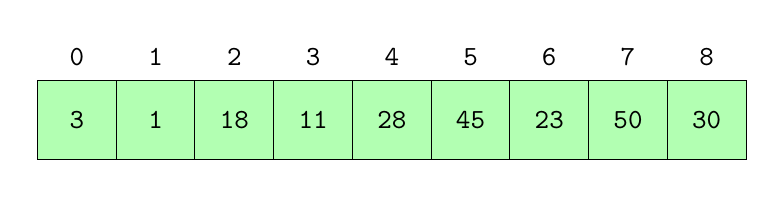
\begin{tikzpicture}[font=\ttfamily,
			array/.style={matrix of nodes,nodes={draw, minimum size=10mm, fill=green!30},column sep=-\pgflinewidth, row sep=0.5mm, nodes in empty cells,
					row 1/.style={nodes={draw=none, fill=none, minimum size=5mm}},
				}]

		\matrix[array] (array) {
			0 & 1 & 2  & 3  & 4  & 5  & 6  & 7  & 8  \\
			3 & 1 & 18 & 11 & 28 & 45 & 23 & 50 & 30 \\
		};
	\end{tikzpicture}
\end{figure}

根据个位数值放入对应的桶中:

\begin{figure}[H]
	\centering
	\begin{tikzpicture}
		\node (a) [cylinder, xshift=0cm, shape border rotate=90, draw, minimum height=15mm, minimum width=10mm] {};
		\node (b) [cylinder, xshift=1.5cm, shape border rotate=90, draw, minimum height=15mm, minimum width=10mm] {};
		\node (c) [cylinder, xshift=3cm, shape border rotate=90, draw, minimum height=15mm, minimum width=10mm] {};
		\node (d) [cylinder, xshift=4.5cm, shape border rotate=90, draw, minimum height=15mm, minimum width=10mm] {};
		\node (e) [cylinder, xshift=6cm, shape border rotate=90, draw, minimum height=15mm, minimum width=10mm] {};
		\node (f) [cylinder, xshift=7.5cm, shape border rotate=90, draw, minimum height=15mm, minimum width=10mm] {};
		\node (g) [cylinder, xshift=9cm, shape border rotate=90, draw, minimum height=15mm, minimum width=10mm] {};
		\node (h) [cylinder, xshift=10.5cm, shape border rotate=90, draw, minimum height=15mm, minimum width=10mm] {};
		\node (i) [cylinder, xshift=12cm, shape border rotate=90, draw, minimum height=15mm, minimum width=10mm] {};
		\node (j) [cylinder, xshift=13.5cm, shape border rotate=90, draw, minimum height=15mm, minimum width=10mm] {};

		\draw (0,-1) node{0};
		\draw (1.5,-1) node{1};
		\draw (3,-1) node{2};
		\draw (4.5,-1) node{3};
		\draw (6,-1) node{4};
		\draw (7.5,-1) node{5};
		\draw (9,-1) node{6};
		\draw (10.5,-1) node{7};
		\draw (12,-1) node{8};
		\draw (13.5,-1) node{9};

		\draw (0,0.3) node{50};
		\draw (0,-0.3) node{30};
		\draw (1.5,0.3) node{1};
		\draw (1.5,-0.3) node{11};
		\draw (4.5,0.3) node{3};
		\draw (4.5,-0.3) node{23};
		\draw (7.5,-0.3) node{45};
		\draw (12,0.3) node{18};
		\draw (12,-0.3) node{28};
	\end{tikzpicture}
\end{figure}

将桶中的元素按顺序赋值到原始数组中:

\begin{figure}[H]
	\centering
	\begin{tikzpicture}[font=\ttfamily,
			array/.style={matrix of nodes,nodes={draw, minimum size=10mm, fill=green!30},column sep=-\pgflinewidth, row sep=0.5mm, nodes in empty cells,
					row 1/.style={nodes={draw=none, fill=none, minimum size=5mm}},
				}]

		\matrix[array] (array) {
			0  & 1  & 2 & 3  & 4 & 5  & 6  & 7  & 8  \\
			50 & 30 & 1 & 11 & 3 & 23 & 45 & 18 & 28 \\
		};
	\end{tikzpicture}
\end{figure}

根据十位数值放入对应的桶中:

\begin{figure}[H]
	\centering
	\begin{tikzpicture}
		\node (a) [cylinder, xshift=0cm, shape border rotate=90, draw, minimum height=15mm, minimum width=10mm] {};
		\node (b) [cylinder, xshift=1.5cm, shape border rotate=90, draw, minimum height=15mm, minimum width=10mm] {};
		\node (c) [cylinder, xshift=3cm, shape border rotate=90, draw, minimum height=15mm, minimum width=10mm] {};
		\node (d) [cylinder, xshift=4.5cm, shape border rotate=90, draw, minimum height=15mm, minimum width=10mm] {};
		\node (e) [cylinder, xshift=6cm, shape border rotate=90, draw, minimum height=15mm, minimum width=10mm] {};
		\node (f) [cylinder, xshift=7.5cm, shape border rotate=90, draw, minimum height=15mm, minimum width=10mm] {};
		\node (g) [cylinder, xshift=9cm, shape border rotate=90, draw, minimum height=15mm, minimum width=10mm] {};
		\node (h) [cylinder, xshift=10.5cm, shape border rotate=90, draw, minimum height=15mm, minimum width=10mm] {};
		\node (i) [cylinder, xshift=12cm, shape border rotate=90, draw, minimum height=15mm, minimum width=10mm] {};
		\node (j) [cylinder, xshift=13.5cm, shape border rotate=90, draw, minimum height=15mm, minimum width=10mm] {};

		\draw (0,-1) node{0};
		\draw (1.5,-1) node{1};
		\draw (3,-1) node{2};
		\draw (4.5,-1) node{3};
		\draw (6,-1) node{4};
		\draw (7.5,-1) node{5};
		\draw (9,-1) node{6};
		\draw (10.5,-1) node{7};
		\draw (12,-1) node{8};
		\draw (13.5,-1) node{9};

		\draw (0,0.3) node{1};
		\draw (0,-0.3) node{3};
		\draw (1.5,0.3) node{11};
		\draw (1.5,-0.3) node{18};
		\draw (3,0.3) node{23};
		\draw (3,-0.3) node{28};
		\draw (4.5,0.3) node{30};
		\draw (4.5,-0.3) node{45};
		\draw (6,-0.3) node{50};
	\end{tikzpicture}
\end{figure}

将桶中的元素按顺序赋值到原始数组中:

\begin{figure}[H]
	\centering
	\begin{tikzpicture}[font=\ttfamily,
			array/.style={matrix of nodes,nodes={draw, minimum size=10mm, fill=green!30},column sep=-\pgflinewidth, row sep=0.5mm, nodes in empty cells,
					row 1/.style={nodes={draw=none, fill=none, minimum size=5mm}},
				}]

		\matrix[array] (array) {
			0 & 1 & 2  & 3  & 4  & 5  & 6  & 7  & 8  \\
			1 & 3 & 11 & 18 & 23 & 28 & 30 & 45 & 50 \\
		};
	\end{tikzpicture}
\end{figure}

\mybox{基数排序}

\begin{lstlisting}[language=Java]
public static void radixSort(int[] arr) {
        int max = arr[0];
        for(int i = 1; i < arr.length; i++) {
            if(arr[i] > max) {
                max = arr[i];
            }
        }

        int bucketNum = 10;
        // 从个位开始
        for(int exp = 1; max / exp > 0; exp *= 10) {
            // 创建桶
            List<LinkedList<Integer>> buckets 
                = new ArrayList<>(bucketNum);
            for(int i = 0; i < bucketNum; i++) {
                buckets.add(new LinkedList<>());
            }

            // 把元素放到对应桶中
            for(int data : arr) {
                int num = (data / exp) % 10;
                buckets.get(num).add(data);
            }

            // 按顺序取出元素
            int cnt = 0;
            for(LinkedList<Integer> bucket : buckets) {
                for(int data : bucket) {
                    arr[cnt++] = data;
                }
            }
        }
    }
\end{lstlisting}

\newpage

\section{珠排序}

\subsection{珠排序(Bead Sort)}

珠排序的算法和算盘非常类似。算盘上有许多圆圆的珠子被串在细杆上,如果把算盘竖起来,算盘上的小珠子会在重力的作用下滑到算盘底部。其中有一个很神奇的细节,如果统计每一横排珠子的数量,下落之后每一排珠子数量正好是下落前珠子数量的升序排序。

\begin{figure}[H]
	\centering
	\begin{tikzpicture}
		\draw[-, very thick] (0,0) -- (0,5);
		\draw[-, very thick] (1,0) -- (1,5);
		\draw[-, very thick] (2,0) -- (2,5);
		\draw[-, very thick] (3,0) -- (3,5);
		\draw[-, very thick] (4,0) -- (4,5);

		\draw (-1,4.5) node{3个};
		\draw (-1,3.5) node{2个};
		\draw (-1,2.5) node{4个};
		\draw (-1,1.5) node{5个};
		\draw (-1,0.5) node{1个};

		\draw[fill=brown] (0,4.5) circle (0.3);
		\draw[fill=brown] (0,3.5) circle (0.3);
		\draw[fill=brown] (0,2.5) circle (0.3);
		\draw[fill=brown] (0,1.5) circle (0.3);
		\draw[fill=brown] (0,0.5) circle (0.3);

		\draw[fill=brown] (1,4.5) circle (0.3);
		\draw[fill=brown] (1,3.5) circle (0.3);
		\draw[fill=brown] (1,2.5) circle (0.3);
		\draw[fill=brown] (1,1.5) circle (0.3);

		\draw[fill=brown] (2,4.5) circle (0.3);
		\draw[fill=brown] (2,2.5) circle (0.3);
		\draw[fill=brown] (2,1.5) circle (0.3);

		\draw[fill=brown] (3,2.5) circle (0.3);
		\draw[fill=brown] (3,1.5) circle (0.3);

		\draw[fill=brown] (4,1.5) circle (0.3);
	\end{tikzpicture}
\end{figure}

\begin{figure}[H]
	\centering
	\begin{tikzpicture}
		\draw[-, very thick] (0,0) -- (0,5);
		\draw[-, very thick] (1,0) -- (1,5);
		\draw[-, very thick] (2,0) -- (2,5);
		\draw[-, very thick] (3,0) -- (3,5);
		\draw[-, very thick] (4,0) -- (4,5);

		\draw (-1,4.5) node{1个};
		\draw (-1,3.5) node{2个};
		\draw (-1,2.5) node{3个};
		\draw (-1,1.5) node{4个};
		\draw (-1,0.5) node{5个};

		\draw[fill=brown] (0,4.5) circle (0.3);
		\draw[fill=brown] (0,3.5) circle (0.3);
		\draw[fill=brown] (0,2.5) circle (0.3);
		\draw[fill=brown] (0,1.5) circle (0.3);
		\draw[fill=brown] (0,0.5) circle (0.3);

		\draw[fill=brown] (1,3.5) circle (0.3);
		\draw[fill=brown] (1,2.5) circle (0.3);
		\draw[fill=brown] (1,1.5) circle (0.3);
		\draw[fill=brown] (1,0.5) circle (0.3);

		\draw[fill=brown] (2,2.5) circle (0.3);
		\draw[fill=brown] (2,1.5) circle (0.3);
		\draw[fill=brown] (2,0.5) circle (0.3);

		\draw[fill=brown] (3,1.5) circle (0.3);
		\draw[fill=brown] (3,0.5) circle (0.3);

		\draw[fill=brown] (4,0.5) circle (0.3);
	\end{tikzpicture}
	\caption{珠子下落}
\end{figure}

通过模拟珠子下落的元素可以对一组正整数进行排序。使用二维数组来模拟算盘,有珠子的位置设为1,没有珠子的位置设为0。例如一个有5个数字组成的无序整型数组\{3, 2, 4, 5, 1\}就可以转化为以下的二维数组:

\begin{table}[H]
	\centering
	\setlength{\tabcolsep}{5mm}{
		\begin{tabular}{|c|c|c|c|c|}
			\hline
			1 & 1 & 1 & 0 & 0 \\
			\hline
			1 & 1 & 0 & 0 & 0 \\
			\hline
			1 & 1 & 1 & 1 & 0 \\
			\hline
			1 & 1 & 1 & 1 & 1 \\
			\hline
			1 & 0 & 0 & 0 & 0 \\
			\hline
		\end{tabular}
	}
	\caption{模拟算盘}
\end{table}

接下来模拟算盘珠子掉落的过程,让所有的元素1都落到二维数组的最底部。

\begin{table}[H]
	\centering
	\setlength{\tabcolsep}{5mm}{
		\begin{tabular}{|c|c|c|c|c|}
			\hline
			1 & 0 & 0 & 0 & 0 \\
			\hline
			1 & 1 & 0 & 0 & 0 \\
			\hline
			1 & 1 & 1 & 0 & 0 \\
			\hline
			1 & 1 & 1 & 1 & 0 \\
			\hline
			1 & 1 & 1 & 1 & 1 \\
			\hline
		\end{tabular}
	}
\end{table}

最后把掉落后的算盘转换为一维有序数组\{1, 2, 3, 4, 5\}。

\newpage

\section{猴子排序}

\subsection{猴子排序(Bogo Sort)}

听说过“猴子和打字机”的理论吗?\\

无限猴子定理(Infinite Monkey Theorem)与薛定谔的猫、电车实验等并居十大思想实验,所谓思想实验即用想象力去进行,而在现实中基本无法去实现的实验。\\

无限猴子定理讲的是如果让一只猴子在打字机上胡乱打字,只要有无限的时间,总有一天可以恰好打出莎士比亚的著作。如果让无限只猴子在无限的空间、无限的时间里不停地敲打打字机,总有一天可以完整打出一本《哈姆雷特》,甚至是可以打出所有可能的文章。

\begin{figure}[H]
	\centering
	
\includegraphics[]{img/C8/8-12/1.png}
	\caption{无限猴子定理}
\end{figure}

这个看似不可能的事情,却可以用现有数学原理被推导出来。但在现实中往往被认为是无法实现的,因为人们认为“无限”这个条件通常无法被满足。根据概率论证,即使可观测宇宙中充满了猴子一直不停地打字,能够打出一部《哈姆雷特》的概率仍然小于$ 1 \over 10^{183900} $。\\

无限猴子定理同样可以用在排序中。如果给数组随机排列顺序,每一次排列之后验证数组是否有序,只要次数足够多,总有一次数组刚好被随机成有序数组。可是要想真的随机出有序数列,恐怕要等到猴年马月了。

\newpage
% \chapter{树}

\section{树}

\subsection{树(Tree)}


% \chapter{图}

\section{图}

\subsection{图(Graph)}

你的微信中有若干好友,而你的好友又有若干好友。许许多多的用户组成了一个多对多的关系网,这个关系网就是数据结构中的图。\\

再例如使用地图导航功能时,导航会根据你的出发地和目的地规划最佳的地铁换乘路线。许许多多的地铁站组成的交通网络也可以认为是图。\\

图是一种比树更为复杂的数据结构。树的结点之间是一对多的关系,并且存在父与子的层级划分。而图的顶点之间是多对多关系,并且所有顶点都是平等的,无所谓谁是父子。\\

在图中,最基本的单元是顶点(vertex),相当于树中的结点。顶点之间的关联关系被称为边(edge)。图中包含一组顶点和一组边,通常用V表示顶点集合,用E表示边集合。边可以看作是顶点对,即$ (v, w) \in E,\ v, w \in V $。\\

在有些图中,每一条边并不是完全等同的。例如地铁线路,站与站之间的距离都有可能不同。因此图中会涉及边的权重(weight),涉及到权重的图被称为带权图(weighted graph),也称为网络。

\begin{figure}[H]
	\centering
	\begin{tikzpicture}
		\begin{scope}[every node/.style={circle,thick,draw}]
			\node (A) at (0,0) {A};
			\node (B) at (0,3) {B};
			\node (C) at (2.5,4) {C};
			\node (D) at (2.5,1) {D};
			\node (E) at (2.5,-3) {E};
			\node (F) at (5,3) {F};
		\end{scope}

		\begin{scope}[>={Stealth[black]},
			every node/.style={fill=white,circle},
			every edge/.style={draw=black,very thick}]
			\path [-] (A) edge node {5} (B);
			\path [-] (B) edge node {3} (C);
			\path [-] (A) edge node {4} (D);
			\path [-] (D) edge node {3} (C);
			\path [-] (A) edge node {3} (E);
			\path [-] (D) edge node {3} (E);
			\path [-] (D) edge node {3} (F);
			\path [-] (C) edge node {5} (F);
			\path [-] (E) edge node {8} (F);
		\end{scope}
	\end{tikzpicture}
	\caption{带权图}
\end{figure}

还有一种图,顶点之间的关联并不是完全对称的。拿微信举例,你的好友列表里有我,但我的好友列表里未必有你。\\

这样一来,顶点之间的边就有了方向的区分,这种带有方向的图被称为有向图(directed graph)。有向边可以使用<v, w>表示从v指向w的边。\\

\begin{figure}[H]
	\centering
	\begin{tikzpicture}
		\begin{scope}[every node/.style={circle,thick,draw}]
			\node (A) at (0,0) {A};
			\node (B) at (0,3) {B};
			\node (C) at (2.5,4) {C};
			\node (D) at (2.5,1) {D};
			\node (E) at (5,0) {E};
		\end{scope}

		\begin{scope}[>={Stealth[black]},
			every node/.style={fill=white,circle},
			every edge/.style={draw=black,very thick}]
			\path [<->] (A) edge node {5} (B);
			\path [->] (B) edge node {3} (C);
			\path [->] (A) edge node {4} (D);
			\path [<->] (D) edge node {3} (C);
			\path [<->] (A) edge node {3} (E);
			\path [->] (D) edge node {3} (E);
		\end{scope}
	\end{tikzpicture}
	\caption{有向图}
\end{figure}

相应地,在QQ中,只要我把你从好友里删除,你在自己的好友列表里就看不到我了。因此QQ的好友关系可以认为是一个没有方向区分的图,这种图被称为无向图(undirected graph)。

\newpage

\section{图的表示}

\subsection{邻接矩阵(Adjacency Matrix)}

拥有n个顶点的图,它所包含的边的数量最多是n(n-1)条,因此,要表达各个顶点之间的关联关系,最清晰易懂的方式是使用邻接矩阵G[N][N]。\\

对于无向图来说,如果顶点之间有关联,那么邻接矩阵中对应的值为1;如果顶点之间没有关联,那么邻接矩阵中对应的值为0。

\vspace{-0.5cm}

\begin{align}\nonumber
	G[i][j] = \begin{cases}
		1 & <v_i, v_j>\text{是G中的边}   \\
		0 & <v_i, v_j>\text{不是G中的边} \\
	\end{cases}
\end{align}

\begin{figure}[H]
	\centering
	\begin{tikzpicture}
		\begin{scope}[every node/.style={circle,thick,draw}]
			\node (A) at (0,0) {A};
			\node (B) at (0,3) {B};
			\node (C) at (2.5,4) {C};
			\node (D) at (2.5,1) {D};
			\node (E) at (4,2) {E};
		\end{scope}

		\begin{scope}[>={Stealth[black]},
			every node/.style={},
			every edge/.style={draw=black,very thick}]
			\path [-] (A) edge node {} (B);
			\path [-] (A) edge node {} (D);
			\path [-] (B) edge node {} (C);
			\path [-] (C) edge node {} (D);
			\path [-] (C) edge node {} (E);
		\end{scope}
	\end{tikzpicture}
\end{figure}

\begin{table}[H]
	\centering
	\setlength{\tabcolsep}{5mm}{
		\begin{tabular}{|c|c|c|c|c|c|}
			\hline
			           & \textbf{A} & \textbf{B} & \textbf{C} & \textbf{D} & \textbf{E} \\
			\hline
			\textbf{A} & 0          & 1          & 0          & 1          & 0          \\
			\hline
			\textbf{B} & 1          & 0          & 1          & 0          & 0          \\
			\hline
			\textbf{C} & 0          & 1          & 0          & 1          & 1          \\
			\hline
			\textbf{D} & 1          & 0          & 1          & 0          & 0          \\
			\hline
			\textbf{E} & 0          & 0          & 1          & 0          & 0          \\
			\hline
		\end{tabular}
	}
	\caption{无向图邻接矩阵}
\end{table}

需要注意的是,邻接矩阵从左上到右下的一条对角线上的元素值必然是0,因为任何一个顶点与它自身是没有连接的。同时,无向图对应的邻接矩阵是一个对称矩阵,假如A和B有关联,那么B和A也必定有关联。\\

但是对于有向图的邻接矩阵,不一定是一个对称矩阵,假如A可以达到B,从B未必能达到A。\\

\begin{figure}[H]
	\centering
	\begin{tikzpicture}
		\begin{scope}[every node/.style={circle,thick,draw}]
			\node (A) at (0,0) {A};
			\node (B) at (0,3) {B};
			\node (C) at (2.5,4) {C};
			\node (D) at (2.5,1) {D};
		\end{scope}

		\begin{scope}[>={Stealth[black]},
			every node/.style={},
			every edge/.style={draw=black,very thick}]
			\path [->] (A) edge node {} (B);
			\path [->] (A) edge node {} (C);
			\path [<->] (C) edge node {} (D);
			\path [->] (D) edge node {} (B);
		\end{scope}
	\end{tikzpicture}
\end{figure}

\begin{table}[H]
	\centering
	\setlength{\tabcolsep}{5mm}{
		\begin{tabular}{|c|c|c|c|c|}
			\hline
			           & \textbf{A} & \textbf{B} & \textbf{C} & \textbf{D} \\
			\hline
			\textbf{A} & 0          & 1          & 1          & 0          \\
			\hline
			\textbf{B} & 0          & 0          & 0          & 0          \\
			\hline
			\textbf{C} & 0          & 0          & 0          & 1          \\
			\hline
			\textbf{D} & 0          & 1          & 1          & 0          \\
			\hline
		\end{tabular}
	}
	\caption{有向图邻接矩阵}
\end{table}

对于网络,只要把邻接矩阵对应位置的值定义为边$ <v_i, v_j> $的权重即可。\\

\begin{figure}[H]
	\centering
	\begin{tikzpicture}
		\begin{scope}[every node/.style={circle,thick,draw}]
			\node (A) at (0,0) {A};
			\node (B) at (3,0) {B};
			\node (C) at (5,2.5) {C};
			\node (D) at (1.5,5) {D};
			\node (E) at (-2,2.5) {E};
			\node (F) at (1.5,2.5) {F};
		\end{scope}

		\begin{scope}[>={Stealth[black]},
			every node/.style={fill=white,circle},
			every edge/.style={draw=black,very thick}]
			\path [->] (A) edge node {5} (B);
			\path [->] (A) edge node {2} (F);
			\path [->] (B) edge node {4} (C);
			\path [->] (C) edge node {9} (D);
			\path [->] (D) edge node {7} (E);
			\path [->] (D) edge node {3} (F);
			\path [->] (E) edge node {1} (A);
			\path [->] (F) edge node {1} (C);
			\path [->] (F) edge node {8} (E);
		\end{scope}
	\end{tikzpicture}
\end{figure}

\begin{table}[H]
	\centering
	\setlength{\tabcolsep}{5mm}{
		\begin{tabular}{|c|c|c|c|c|c|c|}
			\hline
			           & \textbf{A} & \textbf{B} & \textbf{C} & \textbf{D} & \textbf{E} & \textbf{F} \\
			\hline
			\textbf{A} & $ \infty $ & 5          & $ \infty $ & $ \infty $ & $ \infty $ & 2          \\
			\hline
			\textbf{B} & $ \infty $ & $ \infty $ & 4          & $ \infty $ & $ \infty $ & $ \infty $ \\
			\hline
			\textbf{C} & $ \infty $ & $ \infty $ & $ \infty $ & 9          & $ \infty $ & $ \infty $ \\
			\hline
			\textbf{D} & $ \infty $ & $ \infty $ & $ \infty $ & $ \infty $ & 7          & 3          \\
			\hline
			\textbf{E} & 1          & $ \infty $ & $ \infty $ & $ \infty $ & $ \infty $ & $ \infty $ \\
			\hline
			\textbf{F} & $ \infty $ & $ \infty $ & 1          & $ \infty $ & 8          & $ \infty $ \\
			\hline
		\end{tabular}
	}
	\caption{带权图邻接矩阵}
\end{table}

对于带权图,如果$ v_i $和$ v_j $之前没有边应该将权值设为$ \infty $。\\

邻接矩阵的优点:

\begin{enumerate}
	\item 简单、直观。
	\item 可以快速查到一个顶点和另一顶点之间的关联关系。
	\item 方便计算任一顶点的度,对于有向图,从顶点发出的边数为出度,指向顶点的边数为入度。
\end{enumerate}

邻接矩阵的缺点:

\begin{enumerate}
	\item 浪费空间,对于稀疏图(点很多而边很少)有大量无效元素。但对于稠密图(特别是完全图)还是很合算的。
	\item 浪费时间,统计稀疏图中边的个数,也就是计算邻接矩阵中元素1的个数。
\end{enumerate}

\begin{figure}[H]
	\centering
	\begin{tikzpicture}
		\draw[thick,black]  (18:2) \foreach \a in {90,162,234,306} { -- (\a:2) } -- cycle;
		\draw[thick,black] (18:2) \foreach \a in {162,306,90,234} { -- (\a:2) } -- cycle;
		\foreach \a in {18,90,162,234,306} { \node[black,fill=black,circle,inner sep=2pt] at (\a:2){}; }
	\end{tikzpicture}
	\caption{完全图}
\end{figure}

\vspace{0.5cm}

\subsection{邻接表(Adjacency List)}

为了解决邻接矩阵占用空间的问题,人们想到了另一种图的表示方法——邻接表。在邻接表中,图的每一个顶点都是一个链表的头结点,其后连接着该顶点能够直接到达的相邻顶点。对于稀疏图而言,邻接表存储方式占用的空间比邻接矩阵要小得多。\\

\begin{figure}[H]
	\centering
	\begin{tikzpicture}
		\begin{scope}[every node/.style={circle,thick,draw}]
			\node (A) at (0,0) {A};
			\node (B) at (0,3) {B};
			\node (C) at (2.5,4) {C};
			\node (D) at (2.5,1) {D};
		\end{scope}

		\begin{scope}[>={Stealth[black]},
			every node/.style={},
			every edge/.style={draw=black,very thick}]
			\path [->] (A) edge node {} (B);
			\path [->] (A) edge node {} (C);
			\path [<->] (C) edge node {} (D);
			\path [->] (D) edge node {} (A);
		\end{scope}
	\end{tikzpicture}
\end{figure}

\begin{figure}[H]
	\centering
	\begin{tikzpicture}
		\coordinate (0);
		\foreach \t[count=\i from 0,evaluate=\i as\j using int(\i+1)] in {
				1 $ \rightarrow $ 2,
				,
				3,
				1 $ \rightarrow $ 2
			}
		\node at(\i.south)[anchor=north,draw,minimum height=2em,minimum width=1.5em,outer sep=0pt](\j){}
		node at(\j.west)[align=right,left]{\i}
		node at(\j.east)[align=left,right,xshift=-.7em]{$ \rightarrow $ \t};
	\end{tikzpicture}
	\caption{邻接表}
\end{figure}

通过遍历邻接表可以查找到所有能够到达的相邻顶点,但是对于逆向查找,即哪些顶点可以达到一个顶点就会很麻烦。\\

逆邻接表和邻接表是正好相反的,逆邻接表每一个顶点作为链表的头结点,后继结点所存储的是能够直接到达该顶点的相邻顶点。

\begin{figure}[H]
	\centering
	\begin{tikzpicture}
		\coordinate (0);
		\foreach \t[count=\i from 0,evaluate=\i as\j using int(\i+1)] in {
				,
				0 $ \rightarrow $ 3,
				0 $ \rightarrow $ 3,
				2
			}
		\node at(\i.south)[anchor=north,draw,minimum height=2em,minimum width=1.5em,outer sep=0pt](\j){}
		node at(\j.west)[align=right,left]{\i}
		node at(\j.east)[align=left,right,xshift=-.7em]{$ \rightarrow $ \t};
	\end{tikzpicture}
	\caption{逆邻接表}
\end{figure}

可是,一个图要维护正反两个邻接表,也太麻烦了吧?\\

通过十字链表可以把邻接表和逆邻接表结合在一起。\\

\begin{figure}[H]
	\centering
	\begin{tikzpicture}
		\coordinate (0);
		\foreach \t[count=\i from 0,evaluate=\i as\j using int(\i+1)] in {
				1 $ \rightarrow $ 2,
				,
				3,
				1 $ \rightarrow $ 2
			}
		\node at(\i.south)[anchor=north,draw,minimum height=2em,minimum width=1.5em,outer sep=0pt](\j){}
		node at(\j.east)[align=right,left]{\i}
		node at(\j.east)[align=left,right,xshift=-.7em]{$ \rightarrow $ \t};

		\draw (-0.4,-0.5) node{$ \leftarrow $};
		\draw (-1,-1.2) node{$ 3 \leftarrow 0 \leftarrow $};
		\draw (-1,-2) node{$ 3 \leftarrow 0 \leftarrow $};
		\draw (-0.5,-2.9) node{$ 2 \leftarrow $};
	\end{tikzpicture}
	\caption{十字链表}
\end{figure}

\newpage

\section{图的遍历}

\subsection{深度优先搜索(DFS, Depth First Search)}

深度优先搜索是一种一头扎到底的遍历方法,选择一条路,尽可能不断地深入,遇到死路就回退,回退过程中如果遇到没探索的支路,就进入该支路继续深入。\\

例如一个小镇的每个地点都藏有可以实现愿望的光玉,现在要从0号出生点出发去收集所有的光玉。

\begin{figure}[H]
	\centering
	\begin{tikzpicture}
		\begin{scope}[every node/.style={circle,thick,draw}]
			\node (0) at (2.5,4) {0};
			\node (1) at (5,3) {1};
			\node (2) at (2.5,2) {2};
			\node (3) at (1,0) {3};
			\node (4) at (3,0) {4};
			\node (5) at (5,1) {5};
			\node (6) at (6,-1) {6};
			\node (7) at (0,3) {7};
		\end{scope}

		\begin{scope}[>={Stealth[black]},
			every node/.style={},
			every edge/.style={draw=black,very thick}]
			\path [-] (0) edge node {} (1);
			\path [-] (0) edge node {} (2);
			\path [-] (0) edge node {} (7);
			\path [-] (1) edge node {} (4);
			\path [-] (1) edge node {} (5);
			\path [-] (2) edge node {} (4);
			\path [-] (3) edge node {} (4);
			\path [-] (5) edge node {} (6);
		\end{scope}
	\end{tikzpicture}
	\caption{深度优先搜索}
\end{figure}

二叉树的先序遍历本质上也可以认为是图的深度优先遍历。要想实现回溯,可以利用栈的先进后出的特性,也可以采用递归的方式,因为递归本身就是基于方法调用栈来实现的。

\begin{algorithm}[H]
	\caption{深度优先搜索}
	\begin{algorithmic}[1]
		\Procedure{dfs}{Vertex V}
		\State isVisited[V] = true
		\For {v in V}
		\If {!isVisited[v]}
		\State DFS(v)
		\EndIf
		\EndFor
		\EndProcedure
	\end{algorithmic}
\end{algorithm}

\vspace{0.5cm}

\subsection{广度优先搜索(BFS, Breath First Search)}

除了深度优先搜索一头扎到底的方法以外,还有一种方法就是首先把从源点相邻的顶点遍历,然后再遍历稍微远一点的顶点,再去遍历更远一点的顶点。\\

二叉树的层次遍历本质上也可以认为是图的广度优先遍历,需要借助队列来实现重放。

\begin{figure}[H]
	\centering
	\begin{tikzpicture}[
			level distance=1.5cm,
			level 1/.style={sibling distance=4cm},
			level 2/.style={sibling distance=2cm},
			level 3/.style={sibling distance=1cm}
		]
		\node[circle,draw] {1}
		child {
				node[circle,draw] {2}
				child {
						node[circle,draw] {4}
						child {node[circle,draw] {8}}
						child {node[circle,draw] {9}}
					}
				child {
						node[circle,draw] {5}
						child {node[circle,draw] {10}}
						child {node[circle,draw] {11}}
					}
			}
		child {
				node[circle,draw] {3}
				child {
						node[circle,draw] {6}
						child {node[circle,draw] {12}}
						child {node[circle,draw] {13}}
					}
				child {
						node[circle,draw] {7}
						child {node[circle,draw] {14}}
						child {node[circle,draw] {15}}
					}
			};
	\end{tikzpicture}
\end{figure}

\begin{figure}[H]
	\centering
	\begin{tikzpicture}
		\begin{scope}[every node/.style={circle,thick,draw}]
			\node (1) at (0,0) {1};
			\node (2) at (-1,1) {2};
			\node (3) at (1,1) {3};
			\node (4) at (1.5,0) {4};
			\node (5) at (1,-1) {5};
			\node (6) at (-1,-1) {6};
			\node (7) at (-1.5,0) {7};
			\node (8) at (-2,2) {8};
			\node (9) at (-0.5,2) {9};
			\node (10) at (2,2) {10};
			\node (11) at (2.5,1) {11};
			\node (12) at (3,0) {12};
			\node (13) at (2.5,-1) {13};
			\node (14) at (2,-2) {14};
			\node (15) at (0,-2) {15};
			\node (16) at (-2,-2) {16};
			\node (17) at (-2.5,-1) {17};
			\node (18) at (-3,0) {18};
			\node (19) at (-2.5,1) {19};
		\end{scope}

		\begin{scope}[>={Stealth[black]},
			every node/.style={},
			every edge/.style={draw=black,very thick}]
			\path [-] (1) edge node {} (2);
			\path [-] (1) edge node {} (3);
			\path [-] (1) edge node {} (4);
			\path [-] (1) edge node {} (5);
			\path [-] (1) edge node {} (6);
			\path [-] (1) edge node {} (7);
			\path [-] (2) edge node {} (8);
			\path [-] (2) edge node {} (9);
			\path [-] (3) edge node {} (10);
			\path [-] (4) edge node {} (11);
			\path [-] (4) edge node {} (12);
			\path [-] (4) edge node {} (13);
			\path [-] (5) edge node {} (14);
			\path [-] (5) edge node {} (15);
			\path [-] (6) edge node {} (16);
			\path [-] (7) edge node {} (17);
			\path [-] (7) edge node {} (18);
			\path [-] (7) edge node {} (19);
		\end{scope}
	\end{tikzpicture}
	\caption{广度优先搜索}
\end{figure}

\begin{algorithm}[H]
	\caption{广度优先搜索}
	\begin{algorithmic}[1]
		\Procedure{bfs}{Vertex V}
		\State isVisited[V] = true
		\State enqueue(Q, V)
		\While {!isEmpty(Q)}
		\State V = dequeue(Q)
		\For {v in V}
		\If {!isVisited[v]}
		\State isVisited[v] = true
		\State enqueue(Q, v)
		\EndIf
		\EndFor
		\EndWhile
		\EndProcedure
	\end{algorithmic}
\end{algorithm}

\newpage

\section{连通图}

\subsection{连通图}

图还有一些有关路径的术语:

\begin{itemize}
	\item 连通:如果从顶点V到W存在一条路径,则称V和W是连通的。

	\item 路径:顶点V到W的路径是一系列顶点$ \{V, v_1, v_2, \dots, v_n, W\} $的集合,其中任意一对相邻的顶点间都有图中的边。

	\item 路径长度:路径中边的个数,如果是带权图(网络),则是所有边的权重和。

	\item 简单路径:顶点V到W之间的路径中所有顶点都不同。

	\item 回路:起点等于终点的路径。
\end{itemize}

如果图中任意两顶点均连通,那么称这个图是一个连通图。\\

一个图的连通分量指的是图的极大连通子图,极大连通子图需要满足两点要求:

\begin{enumerate}
	\item 顶点数到达极大,即再加一个顶点就不连通了。
	\item 边数达到极大,即包含子图中所有顶点相连的所有边。
\end{enumerate}

\begin{figure}[H]
	\centering
	\begin{tikzpicture}
		\begin{scope}[every node/.style={circle,thick,draw}]
			\node (A) at (0,2) {A};
			\node (B) at (-2,0) {B};
			\node (C) at (0,-2) {C};
			\node (D) at (2,0) {D};
			\node (E) at (-0.75,0) {E};
			\node (F) at (0.75,0) {F};
		\end{scope}

		\begin{scope}[>={Stealth[black]},
			every node/.style={},
			every edge/.style={draw=black,very thick}]
			\path [-] (A) edge node {} (B);
			\path [-] (B) edge node {} (C);
			\path [-] (C) edge node {} (D);
			\path [-] (D) edge node {} (A);
			\path [-] (E) edge node {} (F);
		\end{scope}
	\end{tikzpicture}
	\caption{图G}
\end{figure}

\begin{figure}[H]
	\centering
	\begin{tikzpicture}
		\begin{scope}[every node/.style={circle,thick,draw}]
			\node (A) at (0,2) {A};
			\node (B) at (-2,0) {B};
			\node (C) at (0,-2) {C};
			\node (D) at (2,0) {D};
		\end{scope}

		\begin{scope}[>={Stealth[black]},
			every node/.style={},
			every edge/.style={draw=black,very thick}]
			\path [-] (A) edge node {} (B);
			\path [-] (B) edge node {} (C);
			\path [-] (C) edge node {} (D);
			\path [-] (D) edge node {} (A);
		\end{scope}
	\end{tikzpicture}
	\caption{是图G的极大连通子图}
\end{figure}

\begin{figure}[H]
	\centering
	\begin{tikzpicture}
		\begin{scope}[every node/.style={circle,thick,draw}]
			\node (E) at (-0.75,0) {E};
			\node (F) at (0.75,0) {F};
		\end{scope}

		\begin{scope}[>={Stealth[black]},
			every node/.style={},
			every edge/.style={draw=black,very thick}]
			\path [-] (E) edge node {} (F);
		\end{scope}
	\end{tikzpicture}
	\caption{是图G的极大连通子图}
\end{figure}

\begin{figure}[H]
	\centering
	\begin{tikzpicture}
		\begin{scope}[every node/.style={circle,thick,draw}]
			\node (A) at (0,2) {A};
			\node (B) at (-2,0) {B};
			\node (C) at (0,-2) {C};
			\node (D) at (2,0) {D};
		\end{scope}

		\begin{scope}[>={Stealth[black]},
			every node/.style={},
			every edge/.style={draw=black,very thick}]
			\path [-] (A) edge node {} (B);
			\path [-] (C) edge node {} (D);
			\path [-] (D) edge node {} (A);
		\end{scope}
	\end{tikzpicture}
	\caption{不是图G的极大连通子图}
\end{figure}

\begin{figure}[H]
	\centering
	\begin{tikzpicture}
		\begin{scope}[every node/.style={circle,thick,draw}]
			\node (B) at (-2,0) {B};
			\node (C) at (0,-2) {C};
			\node (D) at (2,0) {D};
		\end{scope}

		\begin{scope}[>={Stealth[black]},
			every node/.style={},
			every edge/.style={draw=black,very thick}]
			\path [-] (B) edge node {} (C);
			\path [-] (C) edge node {} (D);
		\end{scope}
	\end{tikzpicture}
	\caption{不是图G的极大连通子图}
\end{figure}

对于有向图而言,如果有向图中任意一对顶点V和W之间存在双向路径,既可以从$ V $走到$ W $,也可以从$ W $走到$ V $,但这两条路径不一定是同一条,则称该图为强连通图。\\

如果有向图不是强连通图,但将所有的有向边替换为无向边之后可以变为连通图,则称该图为弱连通图。\\

有向图的极大强连通子图称为强连通分量。\\

\begin{figure}[H]
	\centering
	\begin{tikzpicture}
		\begin{scope}[every node/.style={circle,thick,draw}]
			\node (A) at (0,2) {A};
			\node (B) at (-2,0) {B};
			\node (C) at (0,-2) {C};
			\node (D) at (2,0) {D};
		\end{scope}

		\begin{scope}[>={Stealth[black]},
			every node/.style={},
			every edge/.style={draw=black,very thick}]
			\path [->] (A) edge node {} (B);
			\path [->] (B) edge node {} (C);
			\path [->] (C) edge node {} (A);
			\path [->] (A) edge node {} (D);
		\end{scope}
	\end{tikzpicture}
	\caption{有向图G}
\end{figure}

\begin{figure}[H]
	\centering
	\begin{tikzpicture}
		\begin{scope}[every node/.style={circle,thick,draw}]
			\node (A) at (0,2) {A};
			\node (B) at (-2,0) {B};
			\node (C) at (0,-2) {C};
		\end{scope}

		\begin{scope}[>={Stealth[black]},
			every node/.style={},
			every edge/.style={draw=black,very thick}]
			\path [->] (A) edge node {} (B);
			\path [->] (B) edge node {} (C);
			\path [->] (C) edge node {} (A);
		\end{scope}
	\end{tikzpicture}
	\caption{是有向图G的强连通分量}
\end{figure}

\begin{figure}[H]
	\centering
	\begin{tikzpicture}
		\begin{scope}[every node/.style={circle,thick,draw}]
			\node (D) at (2,0) {D};
		\end{scope}
	\end{tikzpicture}
	\caption{是有向图G的强连通分量}
\end{figure}

\vspace{0.5cm}

\subsection{非连通图的遍历}

如果一个图不是连通图,那么无论使用深度优先遍历还是广度优先遍历,都会有顶点无法被访问到。解决这个问题的方式是每调用一次dfs(V)或bfs(V),就把顶点V所在的连通分量遍历一遍。\\

\begin{algorithm}[H]
	\caption{非连通图的深度优先遍历}
	\begin{algorithmic}[1]
		\Procedure{dfs}{Vertex V}
		\State isVisited[V] = true
		\For {v in V}
		\If {!isVisited[v]}
		\State DFS(v)
		\EndIf
		\EndFor
		\EndProcedure
		\\
		\Procedure{listComponents}{Graph G}
		\For {V in G}
		\If {!isVisited[V]}
		\State DFS(V)
		\EndIf
		\EndFor
		\EndProcedure
	\end{algorithmic}
\end{algorithm}

\newpage

\section{最短路径}

\subsection{最短路径(Shortest Path)}

在现实中很多需要都运用到了最短路径的算法,例如从一个地铁站到另一个地铁站的最快换乘路线等。地铁线路图中,地铁站可以看作是图的顶点,站与站之间的线路可以看作是边,权重可以是距离、时间、费用等。\\

\begin{figure}[H]
	\centering
	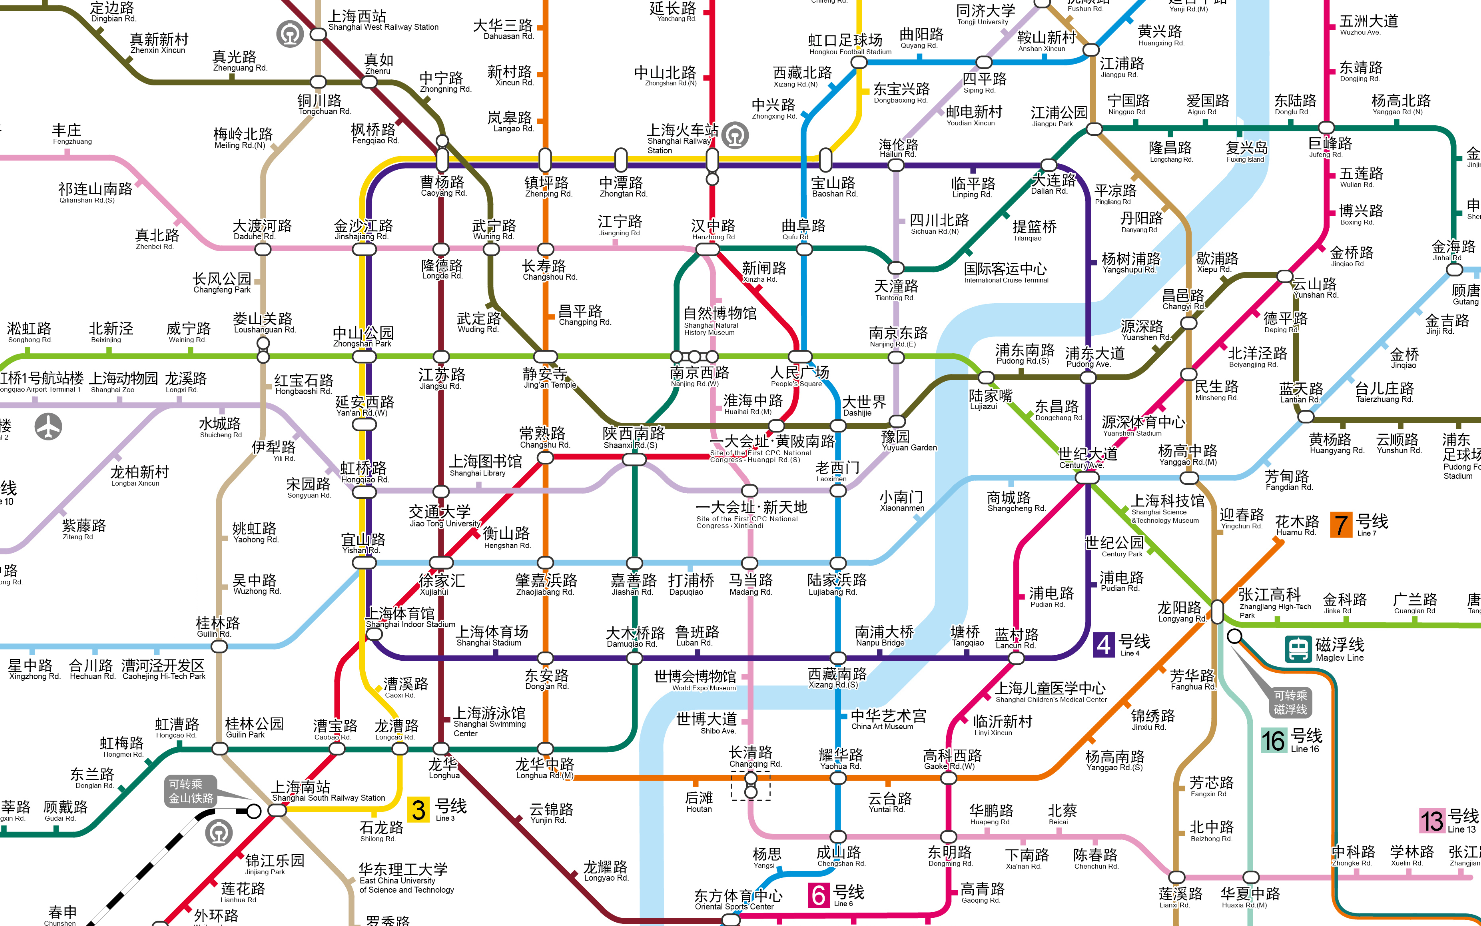
\includegraphics[scale=0.3]{img/C10/10-5/1.png}
	\caption{上海地铁线路图}
\end{figure}

在网络中,求两个不同顶点之间的所有路径中,边的权值之和最小的那一条路径,这条路径就是两点之间的最短路径。其中最短路径的第一个顶点称为源点(source),最后一个顶点为终点(destination)。\\

图的最短路径问题分为2种类型:

\begin{enumerate}
	\item 单源最短路径:从某固定源点出发,求到所有其它顶点的最短路径。
	\item 多源最短路径:求任意两顶点间的最短路径。
\end{enumerate}

\vspace{0.5cm}

\subsection{无权图的单源最短路径算法(SSSP, Single-Source Shortest Path)}

无权图的单源最短路径算法可以按照递增(非递减)的顺序找出到各个顶点的最短路,算法类似广度优先遍历。\\

例如在一个无权图中,以顶点3作为源点,离源点距离为1的顶点有1和6,距离为2的顶点有2和4,距离为3的顶点有5和7。

\begin{figure}[H]
	\centering
	\begin{tikzpicture}
		\begin{scope}[every node/.style={circle,thick,draw}]
			\node (1) at (-1.5,2) {1};
			\node (2) at (1.5,2) {2};
			\node (3) at (-4,0) {3};
			\node (4) at (0,0) {4};
			\node (5) at (4,0) {5};
			\node (6) at (-1.5,-2) {6};
			\node (7) at (1.5,-2) {7};
		\end{scope}

		\begin{scope}[>={Stealth[black]},
			every node/.style={},
			every edge/.style={draw=black,very thick}]
			\path [->] (1) edge node {} (2);
			\path [->] (1) edge node {} (4);
			\path [->] (2) edge node {} (4);
			\path [->] (2) edge node {} (5);
			\path [->] (3) edge node {} (1);
			\path [->] (3) edge node {} (6);
			\path [->] (4) edge node {} (3);
			\path [->] (4) edge node {} (5);
			\path [->] (4) edge node {} (6);
			\path [->] (4) edge node {} (7);
			\path [->] (5) edge node {} (7);
			\path [->] (7) edge node {} (6);
		\end{scope}
	\end{tikzpicture}
\end{figure}

无权图的单元最短路径算法中,dist[v]存储从源点S到v的最短路径,初始化源点dist[S]的距离为0,path[v]表示达到顶点路径v上一个经过的顶点。

\begin{table}[H]
	\centering
	\setlength{\tabcolsep}{5mm}{
		\begin{tabular}{|c|c|c|c|c|c|c|c|}
			\hline
			\textbf{顶点} & \textbf{1} & \textbf{2} & \textbf{3} & \textbf{4} & \textbf{5} & \textbf{6} & \textbf{7} \\
			\hline
			\textbf{dist} & 1          & 2          & 0          & 2          & 3          & 1          & 3          \\
			\hline
			\textbf{path} & 3          & 1          & -1         & 1          & 2          & 3          & 4          \\
			\hline
		\end{tabular}
	}
	\caption{最短路径表}
\end{table}

\begin{algorithm}[H]
	\caption{无权图的单源最短路径}
	\begin{algorithmic}[1]
		\Procedure{unweightedSSSP}{Vertex S}
		\State enqueue(Q, S)
		\While {!isEmpty(Q)}
		\State V = dequeue(Q)
		\For {v in V}
		\If {dist[v] == -1}
		\State dist[v] = dist[V] + 1
		\State path[v] = V
		\State enqueue(Q, v)
		\EndIf
		\EndFor
		\EndWhile
		\EndProcedure
	\end{algorithmic}
\end{algorithm}

\vspace{0.5cm}

\subsection{有权图的单源最短路径算法}

有权图的最短路径不一定是经过顶点树最少的路。如果图中存在负值圈(negative-cost cycle)的话会导致算法失效,因为沿着回路走无穷多次,花销是负无穷。

\begin{figure}[H]
	\centering
	\begin{tikzpicture}
		\begin{scope}[every node/.style={circle,thick,draw}]
			\node (1) at (-1.5,2) {1};
			\node (2) at (1.5,2) {2};
			\node (3) at (-4,0) {3};
			\node (4) at (0,0) {4};
			\node (5) at (4,0) {5};
			\node (6) at (-1.5,-2) {6};
			\node (7) at (1.5,-2) {7};
		\end{scope}

		\begin{scope}[>={Stealth[black]},
			every node/.style={fill=white,circle},
			every edge/.style={draw=black,very thick}]
			\path [->] (1) edge node {2} (2);
			\path [->] (1) edge node {1} (4);
			\path [->, red] (4) edge node {3} (2);
			\path [->, red] (2) edge node {-10} (5);
			\path [->] (3) edge node {4} (1);
			\path [->] (3) edge node {5} (6);
			\path [->] (4) edge node {2} (3);
			\path [->, red] (5) edge node {2} (4);
			\path [->] (4) edge node {8} (6);
			\path [->] (4) edge node {4} (7);
			\path [->] (5) edge node {6} (7);
			\path [->] (7) edge node {1} (6);
		\end{scope}
	\end{tikzpicture}
	\caption{负值圈}
\end{figure}

带权图的单源最短路径可以通过迪杰斯特拉(Dijkstra)算法解决。\\

特斯拉?什么鬼?\\

迪杰斯特拉算法的本质是不断刷新起点与其他各个顶点之间的距离表。Dijkstra算法采用了贪心的思想,每次都未收录的顶点中选取dist值最小的收录。每当收录一个顶点时,可能会影响另外一个顶点的dist值。

\vspace{-0.5cm}

$$
	dist[w] = min\{dist[w], dist[v] + weight_{<v, w>}\}
$$

例如计算从源点A到其它各顶点的最短路径。

\begin{figure}[H]
	\centering
	\begin{tikzpicture}
		\begin{scope}[every node/.style={circle,thick,draw}]
			\node (A) at (-3,2.5) {A};
			\node (B) at (-4,0) {B};
			\node (C) at (0,3) {C};
			\node (D) at (0,0) {D};
			\node (E) at (-1.5,-2.5) {E};
			\node (F) at (2,-1) {F};
			\node (G) at (3,-3) {G};
		\end{scope}

		\begin{scope}[>={Stealth[black]},
			every node/.style={fill=white,circle},
			every edge/.style={draw=black,very thick}]
			\path [-] (A) edge node {5} (B);
			\path [-] (A) edge node {2} (C);
			\path [-] (B) edge node {1} (D);
			\path [-] (B) edge node {6} (E);
			\path [-] (C) edge node {6} (D);
			\path [-] (C) edge node {8} (F);
			\path [-] (E) edge node {1} (D);
			\path [-] (E) edge node {7} (G);
			\path [-] (F) edge node {3} (G);
		\end{scope}
	\end{tikzpicture}
\end{figure}

第1步:创建距离表。其中表中key是顶点名称,value是源点A到对应顶点的已知最短距离。一开始并不知道最短路径是多少,因此value都为$ \infty $。

\begin{table}[H]
	\centering
	\setlength{\tabcolsep}{5mm}{
		\begin{tabular}{|c|c|c|c|c|c|}
			\hline
			\textbf{B} & \textbf{C} & \textbf{D} & \textbf{E} & \textbf{F} & \textbf{G} \\
			\hline
			$ \infty $ & $ \infty $ & $ \infty $ & $ \infty $ & $ \infty $ & $ \infty $ \\
			\hline
		\end{tabular}
	}
\end{table}

第2步:找到源点A的邻接点B和C,从A到B的距离是5,从A到C的距离是2。

\begin{table}[H]
	\centering
	\setlength{\tabcolsep}{5mm}{
		\begin{tabular}{|c|c|c|c|c|c|}
			\hline
			\textbf{B}         & \textbf{C}         & \textbf{D} & \textbf{E} & \textbf{F} & \textbf{G} \\
			\hline
			\textcolor{red}{5} & \textcolor{red}{2} & $ \infty $ & $ \infty $ & $ \infty $ & $ \infty $ \\
			\hline
		\end{tabular}
	}
\end{table}

第3步:从距离表中找到从A出发距离最短的顶点,也就是顶点C。找到顶点C的邻接点D和F(A已经遍历过不需要考虑)。从C到D的距离是6,所以从A到D的距离是2 + 6 = 8;从C到F的距离是8,所以从A到F的距离是2 + 8 = 10。

\begin{table}[H]
	\centering
	\setlength{\tabcolsep}{5mm}{
		\begin{tabular}{|c|c|c|c|c|c|}
			\hline
			\textbf{B} & \textbf{C} & \textbf{D}         & \textbf{E} & \textbf{F}          & \textbf{G} \\
			\hline
			5          & 2          & \textcolor{red}{8} & $ \infty $ & \textcolor{red}{10} & $ \infty $ \\
			\hline
		\end{tabular}
	}
\end{table}

第4步:从距离表中找到从A出发距离最短的顶点(C已经遍历过不需要考虑),也就是顶点B。找到顶点B的邻接点D和E(A已经遍历过不需要考虑)。从B到D的距离是1,所以从A到D的距离是5 + 1 = 6,小于距离表中的8;从B到E的距离是6,所以从A到E的距离是5 + 6 = 11。

\begin{table}[H]
	\centering
	\setlength{\tabcolsep}{5mm}{
		\begin{tabular}{|c|c|c|c|c|c|}
			\hline
			\textbf{B} & \textbf{C} & \textbf{D}         & \textbf{E}          & \textbf{F} & \textbf{G} \\
			\hline
			5          & 2          & \textcolor{red}{6} & \textcolor{red}{11} & 10         & $ \infty $ \\
			\hline
		\end{tabular}
	}
\end{table}

第5步:从距离表中找到从A出发距离最短的顶点(B和C不用考虑),也就是顶点D。找到顶点D的邻接点E和F。从D到E的距离是1,所以从A到E的距离是6 + 1 = 7,小于距离表中的11;从D到F的距离是2,所以从A到F的距离是6 + 2 = 8,小于距离表中的10。

\begin{table}[H]
	\centering
	\setlength{\tabcolsep}{5mm}{
		\begin{tabular}{|c|c|c|c|c|c|}
			\hline
			\textbf{B} & \textbf{C} & \textbf{D} & \textbf{E}         & \textbf{F}         & \textbf{G} \\
			\hline
			5          & 2          & 6          & \textcolor{red}{7} & \textcolor{red}{8} & $ \infty $ \\
			\hline
		\end{tabular}
	}
\end{table}

第6步:从距离表中找到从A出发距离最短的顶点,也就是顶点E。找到顶点E的邻接点G。从E到G的距离是7,所以从A到G的距离是7 + 7 = 14。

\begin{table}[H]
	\centering
	\setlength{\tabcolsep}{5mm}{
		\begin{tabular}{|c|c|c|c|c|c|}
			\hline
			\textbf{B} & \textbf{C} & \textbf{D} & \textbf{E} & \textbf{F} & \textbf{G}          \\
			\hline
			5          & 2          & 6          & 7          & 8          & \textcolor{red}{14} \\
			\hline
		\end{tabular}
	}
\end{table}

第7步:从距离表中找到从A出发距离最短的顶点,也就是顶点F。找到顶点F的邻接点G。从F到G的距离是3,所以从A到G的距离是8 + 3 = 11,小于距离表中的14。

\begin{table}[H]
	\centering
	\setlength{\tabcolsep}{5mm}{
		\begin{tabular}{|c|c|c|c|c|c|}
			\hline
			\textbf{B} & \textbf{C} & \textbf{D} & \textbf{E} & \textbf{F} & \textbf{G}          \\
			\hline
			5          & 2          & 6          & 7          & 8          & \textcolor{red}{11} \\
			\hline
		\end{tabular}
	}
\end{table}

最终,距离表中存储的是从源点A到所有顶点的最短距离。\\

\subsection{多源最短路径算法}

如何能够求出一个带权图中所有顶点两两之间的最短距离呢?\\

对了!刚刚学过了Dijkstra算法,可以对每个顶点都使用一次Dijkstra算法,这样就求出了所有顶点之间的最短距离。\\

这个思路确实可以实现,但是Dijkstra算法的代码逻辑比较复杂,有没有更简单的方法呢?\\

弗洛伊德(Floyd-Warshall)算法是专门用于寻找带权图中多源点之间的最短路径算法。Floyd算法的思想是,若想缩短两点间的距离,仅有一种方式,那就是通过第三顶点绕行。\\

假设$ D^k[i][j] $为路径$ \{i \rightarrow \{l \le k\} \rightarrow j\} $的最小长度。当$ D^{k-1} $已经完成,递推到$ D^k $时:

\begin{enumerate}
	\item 如果$ k \notin \text{最短路径}\{i \rightarrow \{l \le k\} \rightarrow j\} $,则$ D^k = D^{k-1} $。
	\item 如果$ k \in \text{最短路径}\{i \rightarrow \{l \le k\} \rightarrow j\} $,该路径必定由两段最短路径组成,则$ D^k[i][j] = D^{k-1}[i][k] + D^{k-1}[k][j] $。
\end{enumerate}

例如,小哼准备去一些城市旅游,有些城市之间有公路,有些城市之间则没有。为了节省经费以及方便计划旅程,小哼希望在出发之前直到任意两个城市之间的最短路程。\\

如果要让任意两点之间的路程变短,只能引入第三个点,并通过这个顶点中转才有可能缩短原来的路程。这个中转的顶点甚至有时候不只通过一个顶点,而是经过两个或更多点中转会更短。\\

当任意两点之间不允许经过第三个点中转时,这些城市之间的最短路径就是邻接矩阵的初始路径。

\begin{figure}[H]
	\centering
	\begin{tikzpicture}
		\draw (0,0) circle(0.5) node{A};
		\draw (4,0) circle(0.5) node{B};
		\draw (4,4) circle(0.5) node{C};
		\draw (0,4) circle(0.5) node{D};

		\draw[->] (0.5,0) -- (2,0) node[below]{2} -- (3.5,0);
		\draw[->] (0.4,0.25) to[bend right] (3.75,3.6);
		\draw (3,1.5) node{6};
		\draw[->] (3.6,3.75) to[bend right] (0.25,0.4);
		\draw (1,2.5) node{7};
		\draw[->] (0,0.5) -- (0,2) node[left]{4} -- (0,3.5);
		\draw[->] (4,0.5) -- (4,2) node[right]{3} -- (4,3.5);
		\draw[->] (3.5,4) -- (2,4) node[above]{1} -- (0.5,4);
		\draw[->] (-0.5,4) to[bend right] (-0.5,0);
		\draw (-1.5,2) node{5};
		\draw[->] (0,4.5) to[bend left] (4,4.5);
		\draw (2,5.5) node{12};
	\end{tikzpicture}
\end{figure}

\begin{table}[H]
	\centering
	\setlength{\tabcolsep}{5mm}{
		\begin{tabular}{|c|c|c|c|c|}
			\hline
			           & \textbf{A} & \textbf{B} & \textbf{C} & \textbf{D} \\
			\hline
			\textbf{A} & 0          & 2          & 6          & 4          \\
			\hline
			\textbf{B} & $ \infty $ & 0          & 3          & $ \infty $ \\
			\hline
			\textbf{C} & 7          & $ \infty $ & 0          & 1          \\
			\hline
			\textbf{D} & 5          & $ \infty $ & 12         & 0          \\
			\hline
		\end{tabular}
	}
\end{table}

在只允许经过1号顶点中转的情况下,任意两点之间的最短路程更新为:

\begin{table}[H]
	\centering
	\setlength{\tabcolsep}{5mm}{
		\begin{tabular}{|c|c|c|c|c|}
			\hline
			           & \textbf{A} & \textbf{B}         & \textbf{C}          & \textbf{D} \\
			\hline
			\textbf{A} & 0          & 2                  & 6                   & 4          \\
			\hline
			\textbf{B} & $ \infty $ & 0                  & 3                   & $ \infty $ \\
			\hline
			\textbf{C} & 7          & \textcolor{red}{9} & 0                   & 1          \\
			\hline
			\textbf{D} & 5          & \textcolor{red}{7} & \textcolor{red}{11} & 0          \\
			\hline
		\end{tabular}
	}
\end{table}

在只允许经过1号和2号顶点中转的情况下,任意两点之间的最短路程更新为:

\begin{table}[H]
	\centering
	\setlength{\tabcolsep}{5mm}{
		\begin{tabular}{|c|c|c|c|c|}
			\hline
			           & \textbf{A} & \textbf{B} & \textbf{C}          & \textbf{D} \\
			\hline
			\textbf{A} & 0          & 2          & \textcolor{red}{5}  & 4          \\
			\hline
			\textbf{B} & $ \infty $ & 0          & 3                   & $ \infty $ \\
			\hline
			\textbf{C} & 7          & 9          & 0                   & 1          \\
			\hline
			\textbf{D} & 5          & 7          & \textcolor{red}{10} & 0          \\
			\hline
		\end{tabular}
	}
\end{table}

在只允许经过1号、2号和3号顶点中转的情况下,任意两点之间的最短路程更新为:

\begin{table}[H]
	\centering
	\setlength{\tabcolsep}{5mm}{
		\begin{tabular}{|c|c|c|c|c|}
			\hline
			           & \textbf{A}          & \textbf{B} & \textbf{C} & \textbf{D}         \\
			\hline
			\textbf{A} & 0                   & 2          & 5          & 4                  \\
			\hline
			\textbf{B} & \textcolor{red}{10} & 0          & 3          & \textcolor{red}{4} \\
			\hline
			\textbf{C} & 7                   & 9          & 0          & 1                  \\
			\hline
			\textbf{D} & 5                   & 7          & 10         & 0                  \\
			\hline
		\end{tabular}
	}
\end{table}

最后允许通过所有顶点作为中转,任意两点之间的最短路程更新为:

\begin{table}[H]
	\centering
	\setlength{\tabcolsep}{5mm}{
		\begin{tabular}{|c|c|c|c|c|}
			\hline
			           & \textbf{A}         & \textbf{B}         & \textbf{C} & \textbf{D} \\
			\hline
			\textbf{A} & 0                  & 2                  & 5          & 4          \\
			\hline
			\textbf{B} & \textcolor{red}{9} & 0                  & 3          & 4          \\
			\hline
			\textbf{C} & \textcolor{red}{6} & \textcolor{red}{8} & 0          & 1          \\
			\hline
			\textbf{D} & 5                  & 7                  & 10         & 0          \\
			\hline
		\end{tabular}
	}
\end{table}

\mybox{Floyd最短路径}

\begin{lstlisting}[language=C]
void floyd(Graph *g, int dist[MAX][MAX]) {
    // 最短路径矩阵初始化为图的邻接矩阵
    for(int i = 0; i < g->vertexNum; i++) {
        for(int j = 0; j < g->vertexNum; j++) {
            dist[i][j] = g->weight[i][j];
        }
    }

    // Floyd算法
    for(int k = 0; k < g->vertexNum; k++) {
        for(int i = 0; i < g->vertexNum; i++) {
            for(int j = 0; j < g->vertexNum; j++) {
                if(dist[i][k] + dist[k][j] < dist[i][j]) {
                    dist[i][j] = dist[i][k] + dist[k][j];
                }
            }
        }
    }
}
\end{lstlisting}

\newpage

\section{最小生成树}

\subsection{最小生成树(MST, Mininum Spanning Tree)}

所谓最小生成树,就是一个图的极小连通子图,它包含原图的所有顶点,并且所有边的权值之和尽可能小。\\

最小生成树需要满足3个条件:

\begin{enumerate}
	\item 是一棵树:树不能有回路,并且$ |V| $个顶点一定有$ |V| - 1 $条边。

	\item 是生成树:包含原图的全部顶点,树的$ |V| - 1 $条边都必须在图里,并且如果向生成树中任意加一条边都一定构成回路。

	\item 边的权重和最小。
\end{enumerate}

如果最小生成树存在,那么图一定连通,反之亦然。\\

例如一个带权图,蓝色边可以把所有顶点连接起来,又保证边的权值和最小。

\begin{figure}[H]
	\centering
	\begin{tikzpicture}
		\begin{scope}[every node/.style={circle,thick,draw}]
			\node (A) at (-1.5,2) {A};
			\node (B) at (1.5,2) {B};
			\node (C) at (-4,0) {C};
			\node (D) at (0,0) {D};
			\node (E) at (4,0) {E};
			\node (F) at (-1.5,-2) {F};
		\end{scope}

		\begin{scope}[>={Stealth[black]},
			every node/.style={fill=white,circle},
			every edge/.style={draw=black,very thick}]
			\path [->] (B) edge node {7} (E);
			\path [->] (C) edge node {5} (D);
			\path [->] (F) edge node {9} (E);
		\end{scope}

		\begin{scope}[>={Stealth[blue]},
			every node/.style={fill=white,circle},
			every edge/.style={draw=blue,very thick}]
			\path [->] (A) edge node {4} (B);
			\path [->] (A) edge node {3} (C);
			\path [->] (A) edge node {1} (D);
			\path [->] (D) edge node {2} (F);
			\path [->] (D) edge node {3} (E);
		\end{scope}
	\end{tikzpicture}
\end{figure}

\begin{figure}[H]
	\centering
	\begin{tikzpicture}[
			level distance=1.5cm,
			level 1/.style={sibling distance=2cm},
			level 2/.style={sibling distance=1.5cm},
			level 3/.style={sibling distance=1cm}
		]
		\node[circle,draw] {A}
		child {node[circle,draw] {B}}
		child {node[circle,draw] {C}}
		child {
				node[circle,draw] {D}
				child {node[circle,draw] {E}}
				child {node[circle,draw] {F}}
			};
	\end{tikzpicture}
	\caption{最小生成树}
\end{figure}

图的最小生成树不是唯一的,同一个图有可能对应多个最小生成树。\\

最小生成树在现实中很很多用处。假如要在若干个城市之间铺设铁路,而预算又是有限的,那么就需要寻找成本最低的铺设方式。城市之间的交通网就像一个连通图,其实并不需要在每两个城市之间都直接进行连接,只需要一个最小生成树,保证所有的城市都有铁路可以达到即可。\\

\subsection{Prim}

Prim算法是以图的顶点为基础,从一个初始顶点开始,寻找达到其它顶点权值最小的边,并把该顶点加入到已触达顶点的集合中。当全部顶点都加入到集合时,算法的工作就完成了。Prim算法的本质是基于贪心算法(greedy algorithm)。\\

Prim算法可以理解为让一棵小树长大,每次找能够向外生长的最小边。\\

例如使用Prim算法获得一个带权图的最小生成树:

\begin{figure}[H]
	\centering
	\begin{tikzpicture}
		\begin{scope}[every node/.style={circle,thick,draw}]
			\node (A) at (-1.5,2) {A};
			\node (B) at (1.5,2) {B};
			\node (C) at (-4,0) {C};
			\node (D) at (0,0) {D};
			\node (E) at (4,0) {E};
			\node (F) at (-1.5,-2) {F};
			\node (G) at (1.5,-2) {G};
		\end{scope}

		\begin{scope}[>={Stealth[black]},
			every node/.style={fill=white,circle},
			every edge/.style={draw=black,very thick}]
			\path [-] (A) edge node {2} (B);
			\path [-] (A) edge node {1} (D);
			\path [-] (B) edge node {3} (D);
			\path [-] (B) edge node {10} (E);
			\path [-] (C) edge node {4} (A);
			\path [-] (C) edge node {5} (F);
			\path [-] (D) edge node {2} (C);
			\path [-] (D) edge node {7} (E);
			\path [-] (D) edge node {8} (F);
			\path [-] (D) edge node {4} (G);
			\path [-] (E) edge node {6} (G);
			\path [-] (G) edge node {1} (F);
		\end{scope}
	\end{tikzpicture}
\end{figure}

\begin{figure}[H]
	\centering
	\begin{tikzpicture}
		\begin{scope}[every node/.style={circle,thick,draw}]
			\node (A) at (-1.5,2) {\textcolor{red}{A}};
			\node (B) at (1.5,2) {B};
			\node (C) at (-4,0) {C};
			\node (D) at (0,0) {D};
			\node (E) at (4,0) {E};
			\node (F) at (-1.5,-2) {F};
			\node (G) at (1.5,-2) {G};
		\end{scope}

		\begin{scope}[>={Stealth[black]},
			every node/.style={fill=white,circle},
			every edge/.style={draw=black,very thick}]
			\path [-] (A) edge node {2} (B);
			\path [-] (A) edge node {1} (D);
			\path [-] (B) edge node {3} (D);
			\path [-] (B) edge node {10} (E);
			\path [-] (C) edge node {4} (A);
			\path [-] (C) edge node {5} (F);
			\path [-] (D) edge node {2} (C);
			\path [-] (D) edge node {7} (E);
			\path [-] (D) edge node {8} (F);
			\path [-] (D) edge node {4} (G);
			\path [-] (E) edge node {6} (G);
			\path [-] (G) edge node {1} (F);
		\end{scope}
	\end{tikzpicture}
\end{figure}

\begin{figure}[H]
	\centering
	\begin{tikzpicture}
		\begin{scope}[every node/.style={circle,thick,draw}]
			\node (A) at (-1.5,2) {\textcolor{red}{A}};
			\node (B) at (1.5,2) {B};
			\node (C) at (-4,0) {C};
			\node (D) at (0,0) {\textcolor{red}{D}};
			\node (E) at (4,0) {E};
			\node (F) at (-1.5,-2) {F};
			\node (G) at (1.5,-2) {G};
		\end{scope}

		\begin{scope}[>={Stealth[black]},
			every node/.style={fill=white,circle},
			every edge/.style={draw=black,very thick}]
			\path [-] (A) edge node {2} (B);
			\path [-] (B) edge node {3} (D);
			\path [-] (B) edge node {10} (E);
			\path [-] (C) edge node {4} (A);
			\path [-] (C) edge node {5} (F);
			\path [-] (D) edge node {2} (C);
			\path [-] (D) edge node {7} (E);
			\path [-] (D) edge node {8} (F);
			\path [-] (D) edge node {4} (G);
			\path [-] (E) edge node {6} (G);
			\path [-] (G) edge node {1} (F);
		\end{scope}

		\begin{scope}[>={Stealth[red]},
			every node/.style={fill=white,circle},
			every edge/.style={draw=red,very thick}]
			\path [-] (A) edge node {1} (D);
		\end{scope}
	\end{tikzpicture}
\end{figure}

\begin{figure}[H]
	\centering
	\begin{tikzpicture}
		\begin{scope}[every node/.style={circle,thick,draw}]
			\node (A) at (-1.5,2) {\textcolor{red}{A}};
			\node (B) at (1.5,2) {\textcolor{red}{B}};
			\node (C) at (-4,0) {C};
			\node (D) at (0,0) {\textcolor{red}{D}};
			\node (E) at (4,0) {E};
			\node (F) at (-1.5,-2) {F};
			\node (G) at (1.5,-2) {G};
		\end{scope}

		\begin{scope}[>={Stealth[black]},
			every node/.style={fill=white,circle},
			every edge/.style={draw=black,very thick}]
			\path [-] (B) edge node {3} (D);
			\path [-] (B) edge node {10} (E);
			\path [-] (C) edge node {4} (A);
			\path [-] (C) edge node {5} (F);
			\path [-] (D) edge node {2} (C);
			\path [-] (D) edge node {7} (E);
			\path [-] (D) edge node {8} (F);
			\path [-] (D) edge node {4} (G);
			\path [-] (E) edge node {6} (G);
			\path [-] (G) edge node {1} (F);
		\end{scope}

		\begin{scope}[>={Stealth[red]},
			every node/.style={fill=white,circle},
			every edge/.style={draw=red,very thick}]
			\path [-] (A) edge node {1} (D);
			\path [-] (A) edge node {2} (B);
		\end{scope}
	\end{tikzpicture}
\end{figure}

\begin{figure}[H]
	\centering
	\begin{tikzpicture}
		\begin{scope}[every node/.style={circle,thick,draw}]
			\node (A) at (-1.5,2) {\textcolor{red}{A}};
			\node (B) at (1.5,2) {\textcolor{red}{B}};
			\node (C) at (-4,0) {\textcolor{red}{C}};
			\node (D) at (0,0) {\textcolor{red}{D}};
			\node (E) at (4,0) {E};
			\node (F) at (-1.5,-2) {F};
			\node (G) at (1.5,-2) {G};
		\end{scope}

		\begin{scope}[>={Stealth[black]},
			every node/.style={fill=white,circle},
			every edge/.style={draw=black,very thick}]
			\path [-] (B) edge node {3} (D);
			\path [-] (B) edge node {10} (E);
			\path [-] (C) edge node {4} (A);
			\path [-] (C) edge node {5} (F);
			\path [-] (D) edge node {7} (E);
			\path [-] (D) edge node {8} (F);
			\path [-] (D) edge node {4} (G);
			\path [-] (E) edge node {6} (G);
			\path [-] (G) edge node {1} (F);
		\end{scope}

		\begin{scope}[>={Stealth[red]},
			every node/.style={fill=white,circle},
			every edge/.style={draw=red,very thick}]
			\path [-] (A) edge node {1} (D);
			\path [-] (A) edge node {2} (B);
			\path [-] (D) edge node {2} (C);
		\end{scope}
	\end{tikzpicture}
\end{figure}

\begin{figure}[H]
	\centering
	\begin{tikzpicture}
		\begin{scope}[every node/.style={circle,thick,draw}]
			\node (A) at (-1.5,2) {\textcolor{red}{A}};
			\node (B) at (1.5,2) {\textcolor{red}{B}};
			\node (C) at (-4,0) {\textcolor{red}{C}};
			\node (D) at (0,0) {\textcolor{red}{D}};
			\node (E) at (4,0) {E};
			\node (F) at (-1.5,-2) {F};
			\node (G) at (1.5,-2) {\textcolor{red}{G}};
		\end{scope}

		\begin{scope}[>={Stealth[black]},
			every node/.style={fill=white,circle},
			every edge/.style={draw=black,very thick}]
			\path [-] (B) edge node {3} (D);
			\path [-] (B) edge node {10} (E);
			\path [-] (C) edge node {4} (A);
			\path [-] (C) edge node {5} (F);
			\path [-] (D) edge node {7} (E);
			\path [-] (D) edge node {8} (F);
			\path [-] (E) edge node {6} (G);
			\path [-] (G) edge node {1} (F);
		\end{scope}

		\begin{scope}[>={Stealth[red]},
			every node/.style={fill=white,circle},
			every edge/.style={draw=red,very thick}]
			\path [-] (A) edge node {1} (D);
			\path [-] (A) edge node {2} (B);
			\path [-] (D) edge node {2} (C);
			\path [-] (D) edge node {4} (G);
		\end{scope}
	\end{tikzpicture}
\end{figure}

\begin{figure}[H]
	\centering
	\begin{tikzpicture}
		\begin{scope}[every node/.style={circle,thick,draw}]
			\node (A) at (-1.5,2) {\textcolor{red}{A}};
			\node (B) at (1.5,2) {\textcolor{red}{B}};
			\node (C) at (-4,0) {\textcolor{red}{C}};
			\node (D) at (0,0) {\textcolor{red}{D}};
			\node (E) at (4,0) {E};
			\node (F) at (-1.5,-2) {\textcolor{red}{F}};
			\node (G) at (1.5,-2) {\textcolor{red}{G}};
		\end{scope}

		\begin{scope}[>={Stealth[black]},
			every node/.style={fill=white,circle},
			every edge/.style={draw=black,very thick}]
			\path [-] (B) edge node {3} (D);
			\path [-] (B) edge node {10} (E);
			\path [-] (C) edge node {4} (A);
			\path [-] (C) edge node {5} (F);
			\path [-] (D) edge node {7} (E);
			\path [-] (D) edge node {8} (F);
			\path [-] (E) edge node {6} (G);
		\end{scope}

		\begin{scope}[>={Stealth[red]},
			every node/.style={fill=white,circle},
			every edge/.style={draw=red,very thick}]
			\path [-] (A) edge node {1} (D);
			\path [-] (A) edge node {2} (B);
			\path [-] (D) edge node {2} (C);
			\path [-] (D) edge node {4} (G);
			\path [-] (G) edge node {1} (F);
		\end{scope}
	\end{tikzpicture}
\end{figure}

\begin{figure}[H]
	\centering
	\begin{tikzpicture}
		\begin{scope}[every node/.style={circle,thick,draw}]
			\node (A) at (-1.5,2) {\textcolor{red}{A}};
			\node (B) at (1.5,2) {\textcolor{red}{B}};
			\node (C) at (-4,0) {\textcolor{red}{C}};
			\node (D) at (0,0) {\textcolor{red}{D}};
			\node (E) at (4,0) {\textcolor{red}{E}};
			\node (F) at (-1.5,-2) {\textcolor{red}{F}};
			\node (G) at (1.5,-2) {\textcolor{red}{G}};
		\end{scope}

		\begin{scope}[>={Stealth[black]},
			every node/.style={fill=white,circle},
			every edge/.style={draw=black,very thick}]
			\path [-] (B) edge node {3} (D);
			\path [-] (B) edge node {10} (E);
			\path [-] (C) edge node {4} (A);
			\path [-] (C) edge node {5} (F);
			\path [-] (D) edge node {7} (E);
			\path [-] (D) edge node {8} (F);
		\end{scope}

		\begin{scope}[>={Stealth[red]},
			every node/.style={fill=white,circle},
			every edge/.style={draw=red,very thick}]
			\path [-] (A) edge node {1} (D);
			\path [-] (A) edge node {2} (B);
			\path [-] (D) edge node {2} (C);
			\path [-] (D) edge node {4} (G);
			\path [-] (G) edge node {1} (F);
			\path [-] (E) edge node {6} (G);
		\end{scope}
	\end{tikzpicture}
\end{figure}

\vspace{0.5cm}

\subsection{Kruskal}

与Prim算法不同,Prim算法是以顶点为关键来获得最小生成树的,而Kruskal算法是以边为关键获得最小生成树的。\\

Kruskal算法可以理解为将森林合并成树,每次在图中找权值最小的边收录。\\

例如使用Kruskal算法获得一个带权图的最小生成树:

\begin{figure}[H]
	\centering
	\begin{tikzpicture}
		\begin{scope}[every node/.style={circle,thick,draw}]
			\node (A) at (-1.5,2) {\textcolor{red}{A}};
			\node (B) at (1.5,2) {B};
			\node (C) at (-4,0) {C};
			\node (D) at (0,0) {\textcolor{red}{D}};
			\node (E) at (4,0) {E};
			\node (F) at (-1.5,-2) {F};
			\node (G) at (1.5,-2) {G};
		\end{scope}

		\begin{scope}[>={Stealth[black]},
			every node/.style={fill=white,circle},
			every edge/.style={draw=black,very thick}]
			\path [-] (A) edge node {2} (B);
			\path [-] (B) edge node {3} (D);
			\path [-] (B) edge node {10} (E);
			\path [-] (C) edge node {4} (A);
			\path [-] (C) edge node {5} (F);
			\path [-] (D) edge node {2} (C);
			\path [-] (D) edge node {7} (E);
			\path [-] (D) edge node {8} (F);
			\path [-] (D) edge node {4} (G);
			\path [-] (E) edge node {6} (G);
			\path [-] (G) edge node {1} (F);
		\end{scope}

		\begin{scope}[>={Stealth[red]},
			every node/.style={fill=white,circle},
			every edge/.style={draw=red,very thick}]
			\path [-] (A) edge node {1} (D);
		\end{scope}
	\end{tikzpicture}
\end{figure}

\begin{figure}[H]
	\centering
	\begin{tikzpicture}
		\begin{scope}[every node/.style={circle,thick,draw}]
			\node (A) at (-1.5,2) {\textcolor{red}{A}};
			\node (B) at (1.5,2) {B};
			\node (C) at (-4,0) {C};
			\node (D) at (0,0) {\textcolor{red}{D}};
			\node (E) at (4,0) {E};
			\node (F) at (-1.5,-2) {\textcolor{red}{F}};
			\node (G) at (1.5,-2) {\textcolor{red}{G}};
		\end{scope}

		\begin{scope}[>={Stealth[black]},
			every node/.style={fill=white,circle},
			every edge/.style={draw=black,very thick}]
			\path [-] (A) edge node {2} (B);
			\path [-] (B) edge node {3} (D);
			\path [-] (B) edge node {10} (E);
			\path [-] (C) edge node {4} (A);
			\path [-] (C) edge node {5} (F);
			\path [-] (D) edge node {2} (C);
			\path [-] (D) edge node {7} (E);
			\path [-] (D) edge node {8} (F);
			\path [-] (D) edge node {4} (G);
			\path [-] (E) edge node {6} (G);
		\end{scope}

		\begin{scope}[>={Stealth[red]},
			every node/.style={fill=white,circle},
			every edge/.style={draw=red,very thick}]
			\path [-] (A) edge node {1} (D);
			\path [-] (G) edge node {1} (F);
		\end{scope}
	\end{tikzpicture}
\end{figure}

\begin{figure}[H]
	\centering
	\begin{tikzpicture}
		\begin{scope}[every node/.style={circle,thick,draw}]
			\node (A) at (-1.5,2) {\textcolor{red}{A}};
			\node (B) at (1.5,2) {B};
			\node (C) at (-4,0) {\textcolor{red}{C}};
			\node (D) at (0,0) {\textcolor{red}{D}};
			\node (E) at (4,0) {E};
			\node (F) at (-1.5,-2) {\textcolor{red}{F}};
			\node (G) at (1.5,-2) {\textcolor{red}{G}};
		\end{scope}

		\begin{scope}[>={Stealth[black]},
			every node/.style={fill=white,circle},
			every edge/.style={draw=black,very thick}]
			\path [-] (A) edge node {2} (B);
			\path [-] (B) edge node {3} (D);
			\path [-] (B) edge node {10} (E);
			\path [-] (C) edge node {4} (A);
			\path [-] (C) edge node {5} (F);
			\path [-] (D) edge node {7} (E);
			\path [-] (D) edge node {8} (F);
			\path [-] (D) edge node {4} (G);
			\path [-] (E) edge node {6} (G);
		\end{scope}

		\begin{scope}[>={Stealth[red]},
			every node/.style={fill=white,circle},
			every edge/.style={draw=red,very thick}]
			\path [-] (A) edge node {1} (D);
			\path [-] (G) edge node {1} (F);
			\path [-] (D) edge node {2} (C);
		\end{scope}
	\end{tikzpicture}
\end{figure}

\begin{figure}[H]
	\centering
	\begin{tikzpicture}
		\begin{scope}[every node/.style={circle,thick,draw}]
			\node (A) at (-1.5,2) {\textcolor{red}{A}};
			\node (B) at (1.5,2) {\textcolor{red}{B}};
			\node (C) at (-4,0) {\textcolor{red}{C}};
			\node (D) at (0,0) {\textcolor{red}{D}};
			\node (E) at (4,0) {E};
			\node (F) at (-1.5,-2) {\textcolor{red}{F}};
			\node (G) at (1.5,-2) {\textcolor{red}{G}};
		\end{scope}

		\begin{scope}[>={Stealth[black]},
			every node/.style={fill=white,circle},
			every edge/.style={draw=black,very thick}]
			\path [-] (B) edge node {3} (D);
			\path [-] (B) edge node {10} (E);
			\path [-] (C) edge node {4} (A);
			\path [-] (C) edge node {5} (F);
			\path [-] (D) edge node {7} (E);
			\path [-] (D) edge node {8} (F);
			\path [-] (D) edge node {4} (G);
			\path [-] (E) edge node {6} (G);
		\end{scope}

		\begin{scope}[>={Stealth[red]},
			every node/.style={fill=white,circle},
			every edge/.style={draw=red,very thick}]
			\path [-] (A) edge node {1} (D);
			\path [-] (G) edge node {1} (F);
			\path [-] (D) edge node {2} (C);
			\path [-] (A) edge node {2} (B);
		\end{scope}
	\end{tikzpicture}
\end{figure}

\begin{figure}[H]
	\centering
	\begin{tikzpicture}
		\begin{scope}[every node/.style={circle,thick,draw}]
			\node (A) at (-1.5,2) {\textcolor{red}{A}};
			\node (B) at (1.5,2) {\textcolor{red}{B}};
			\node (C) at (-4,0) {\textcolor{red}{C}};
			\node (D) at (0,0) {\textcolor{red}{D}};
			\node (E) at (4,0) {E};
			\node (F) at (-1.5,-2) {\textcolor{red}{F}};
			\node (G) at (1.5,-2) {\textcolor{red}{G}};
		\end{scope}

		\begin{scope}[>={Stealth[black]},
			every node/.style={fill=white,circle},
			every edge/.style={draw=black,very thick}]
			\path [-] (B) edge node {3} (D);
			\path [-] (B) edge node {10} (E);
			\path [-] (C) edge node {4} (A);
			\path [-] (C) edge node {5} (F);
			\path [-] (D) edge node {7} (E);
			\path [-] (D) edge node {8} (F);
			\path [-] (E) edge node {6} (G);
		\end{scope}

		\begin{scope}[>={Stealth[red]},
			every node/.style={fill=white,circle},
			every edge/.style={draw=red,very thick}]
			\path [-] (A) edge node {1} (D);
			\path [-] (G) edge node {1} (F);
			\path [-] (D) edge node {2} (C);
			\path [-] (A) edge node {2} (B);
			\path [-] (D) edge node {4} (G);
		\end{scope}
	\end{tikzpicture}
\end{figure}

\begin{figure}[H]
	\centering
	\begin{tikzpicture}
		\begin{scope}[every node/.style={circle,thick,draw}]
			\node (A) at (-1.5,2) {\textcolor{red}{A}};
			\node (B) at (1.5,2) {\textcolor{red}{B}};
			\node (C) at (-4,0) {\textcolor{red}{C}};
			\node (D) at (0,0) {\textcolor{red}{D}};
			\node (E) at (4,0) {\textcolor{red}{E}};
			\node (F) at (-1.5,-2) {\textcolor{red}{F}};
			\node (G) at (1.5,-2) {\textcolor{red}{G}};
		\end{scope}

		\begin{scope}[>={Stealth[black]},
			every node/.style={fill=white,circle},
			every edge/.style={draw=black,very thick}]
			\path [-] (B) edge node {3} (D);
			\path [-] (B) edge node {10} (E);
			\path [-] (C) edge node {4} (A);
			\path [-] (C) edge node {5} (F);
			\path [-] (D) edge node {7} (E);
			\path [-] (D) edge node {8} (F);
		\end{scope}

		\begin{scope}[>={Stealth[red]},
			every node/.style={fill=white,circle},
			every edge/.style={draw=red,very thick}]
			\path [-] (A) edge node {1} (D);
			\path [-] (G) edge node {1} (F);
			\path [-] (D) edge node {2} (C);
			\path [-] (A) edge node {2} (B);
			\path [-] (D) edge node {4} (G);
			\path [-] (E) edge node {6} (G);
		\end{scope}
	\end{tikzpicture}
\end{figure}

\newpage

\section{拓扑排序}

\subsection{拓扑排序(Topological Sort)}

一项大的工程常被分为多个小的子工程,子工程之间可能存在一定的先后顺序,即某些子工程必须在其它的一些子工程完成后才能开始。在现代化管理中,有向图可以用来描述和分析一项工程的计划和实施过程,其中图的顶点表示活动,有向边表示活动之间的先后关系,这样的图称为AOV(Activity on Vertex)网。

\begin{figure}[H]
	\centering
	\begin{tikzpicture}
		\begin{scope}[every node/.style={circle,thick,draw}]
			\node (A) at (0,0) {A};
			\node (B) at (2,0) {B};
			\node (C) at (3.5,1.5) {C};
			\node (D) at (3.5,-1.5) {D};
			\node (E) at (5,0) {E};
			\node (F) at (7,0){F};
		\end{scope}

		\begin{scope}[>={Stealth[black]},
			every node/.style={},
			every edge/.style={draw=black,very thick}]
			\path [->] (A) edge node {} (B);
			\path [->] (B) edge node {} (C);
			\path [->] (B) edge node {} (D);
			\path [->] (C) edge node {} (E);
			\path [->] (B) edge node {} (E);
			\path [->] (D) edge node {} (E);
			\path [->] (E) edge node {} (F);
		\end{scope}
	\end{tikzpicture}
	\caption{AOV网}
\end{figure}

如果图中从顶点V到W有一条有向路径,则V一定排在W之前,满足此条件的顶点序列称为一个拓扑序。AOV网如果有合理的拓扑序,则必定是有向无环图(DAG, Directed Acyclic Graph)。\\

可以使用卡恩Kahn算法完成拓扑排序。假设列表$ L $用于存放拓扑排序的结果,把所有入度为0的顶点放入L中,然后把这些顶点从图中去掉。重复该操作,直到找不到入度为0的顶点。如果此时L中的元素个数和图的顶点总数相同,说明拓扑排序完成;如果此时L中的元素个数少于图的顶点总数,说明原图中存在环,无法进行拓扑排序。\\

例如对计算机专业课安排学习顺序:

\begin{table}[H]
	\centering
	\setlength{\tabcolsep}{5mm}{
		\begin{tabular}{|c|c|c|}
			\hline
			\textbf{课程代码} & \textbf{课程名称}    & \textbf{预修课程} \\
			\hline
			C1                & 程序设计基础         & 无                \\
			\hline
			C2                & 离散数学             & 无                \\
			\hline
			C3                & 数据结构             & C1、C2            \\
			\hline
			C4                & 微积分(一)         & 无                \\
			\hline
			C5                & 微积分(二)         & C4                \\
			\hline
			C6                & 线性代数             & C5                \\
			\hline
			C7                & 算法分析与设计       & C3                \\
			\hline
			C8                & 逻辑与计算机设计基础 & 无                \\
			\hline
			C9                & 计算机组成           & C8                \\
			\hline
			C10               & 操作系统             & C7、C9            \\
			\hline
			C11               & 编译原理             & C7、C9            \\
			\hline
			C12               & 数据库               & C7                \\
			\hline
			C13               & 计算理论             & C2                \\
			\hline
			C14               & 计算机网络           & C10               \\
			\hline
			C15               & 数值分析             & C6                \\
			\hline
		\end{tabular}
	}
	\caption{计算机专业课}
\end{table}

\begin{figure}[H]
	\centering
	\begin{tikzpicture}
		\begin{scope}[every node/.style={circle,thick,draw}]
			\node (C1) at (0,6) {C1};
			\node (C2) at (0,4) {C2};
			\node (C3) at (2,5) {C3};
			\node (C4) at (0,0) {C4};
			\node (C5) at (2,0) {C5};
			\node (C6) at (4,0) {C6};
			\node (C7) at (4,5) {C7};
			\node (C8) at (0,2) {C8};
			\node (C9) at (2,2) {C9};
			\node (C10) at (6,3) {C10};
			\node (C11) at (4.5,1.5) {C11};
			\node (C12) at (6,5) {C12};
			\node (C13) at (3,3.5) {C13};
			\node (C14) at (8,3) {C14};
			\node (C15) at (6,0) {C15};
		\end{scope}

		\begin{scope}[>={Stealth[black]},
			every node/.style={},
			every edge/.style={draw=black,very thick}]
			\path [->] (C1) edge node {} (C3);
			\path [->] (C2) edge node {} (C3);
			\path [->] (C2) edge node {} (C13);
			\path [->] (C3) edge node {} (C7);
			\path [->] (C7) edge node {} (C12);
			\path [->] (C7) edge node {} (C10);
			\path [->] (C7) edge node {} (C11);
			\path [->] (C8) edge node {} (C9);
			\path [->] (C9) edge node {} (C10);
			\path [->] (C9) edge node {} (C11);
			\path [->] (C4) edge node {} (C5);
			\path [->] (C5) edge node {} (C6);
			\path [->] (C6) edge node {} (C15);
			\path [->] (C10) edge node {} (C14);
		\end{scope}
	\end{tikzpicture}
	\caption{计算机专业课AOV网}
\end{figure}

\begin{figure}[H]
	\centering
	\begin{tikzpicture}
		\begin{scope}[every node/.style={circle,thick,draw}]
			\node (C3) at (2,5) {C3};
			\node (C5) at (2,0) {C5};
			\node (C6) at (4,0) {C6};
			\node (C7) at (4,5) {C7};
			\node (C9) at (2,2) {C9};
			\node (C10) at (6,3) {C10};
			\node (C11) at (4.5,1.5) {C11};
			\node (C12) at (6,5) {C12};
			\node (C13) at (3,3.5) {C13};
			\node (C14) at (8,3) {C14};
			\node (C15) at (6,0) {C15};
		\end{scope}

		\begin{scope}[>={Stealth[black]},
			every node/.style={},
			every edge/.style={draw=black,very thick}]
			\path [->] (C3) edge node {} (C7);
			\path [->] (C7) edge node {} (C12);
			\path [->] (C7) edge node {} (C10);
			\path [->] (C7) edge node {} (C11);
			\path [->] (C9) edge node {} (C10);
			\path [->] (C9) edge node {} (C11);
			\path [->] (C5) edge node {} (C6);
			\path [->] (C6) edge node {} (C15);
			\path [->] (C10) edge node {} (C14);
		\end{scope}
	\end{tikzpicture}
\end{figure}

\begin{table}[H]
	\centering
	\setlength{\tabcolsep}{5mm}{
		\begin{tabular}{|c|c|}
			\hline
			\textbf{学期}     & \textbf{课程}  \\
			\hline
			\textbf{第一学期} & C1、C2、C4、C8 \\
			\hline
		\end{tabular}
	}
	\caption{第一学期课程}
\end{table}

\begin{figure}[H]
	\centering
	\begin{tikzpicture}
		\begin{scope}[every node/.style={circle,thick,draw}]
			\node (C6) at (4,0) {C6};
			\node (C7) at (4,5) {C7};
			\node (C10) at (6,3) {C10};
			\node (C11) at (4.5,1.5) {C11};
			\node (C12) at (6,5) {C12};
			\node (C14) at (8,3) {C14};
			\node (C15) at (6,0) {C15};
		\end{scope}

		\begin{scope}[>={Stealth[black]},
			every node/.style={},
			every edge/.style={draw=black,very thick}]
			\path [->] (C7) edge node {} (C12);
			\path [->] (C7) edge node {} (C10);
			\path [->] (C7) edge node {} (C11);
			\path [->] (C6) edge node {} (C15);
			\path [->] (C10) edge node {} (C14);
		\end{scope}
	\end{tikzpicture}
\end{figure}

\begin{table}[H]
	\centering
	\setlength{\tabcolsep}{5mm}{
		\begin{tabular}{|c|c|}
			\hline
			\textbf{学期}     & \textbf{课程}   \\
			\hline
			\textbf{第一学期} & C1、C2、C4、C8  \\
			\hline
			\textbf{第二学期} & C3、C5、C9、C13 \\
			\hline
		\end{tabular}
	}
	\caption{第二学期课程}
\end{table}

\begin{figure}[H]
	\centering
	\begin{tikzpicture}
		\begin{scope}[every node/.style={circle,thick,draw}]
			\node (C10) at (6,3) {C10};
			\node (C11) at (4.5,1.5) {C11};
			\node (C12) at (6,5) {C12};
			\node (C14) at (8,3) {C14};
			\node (C15) at (6,0) {C15};
		\end{scope}

		\begin{scope}[>={Stealth[black]},
			every node/.style={},
			every edge/.style={draw=black,very thick}]
			\path [->] (C10) edge node {} (C14);
		\end{scope}
	\end{tikzpicture}
\end{figure}

\begin{table}[H]
	\centering
	\setlength{\tabcolsep}{5mm}{
		\begin{tabular}{|c|c|}
			\hline
			\textbf{学期}     & \textbf{课程}   \\
			\hline
			\textbf{第一学期} & C1、C2、C4、C8  \\
			\hline
			\textbf{第二学期} & C3、C5、C9、C13 \\
			\hline
			\textbf{第三学期} & C6、C7          \\
			\hline
		\end{tabular}
	}
	\caption{第三学期课程}
\end{table}

\begin{figure}[H]
	\centering
	\begin{tikzpicture}
		\begin{scope}[every node/.style={circle,thick,draw}]
			\node (C14) at (8,3) {C14};
		\end{scope}
	\end{tikzpicture}
\end{figure}

\begin{table}[H]
	\centering
	\setlength{\tabcolsep}{5mm}{
		\begin{tabular}{|c|c|}
			\hline
			\textbf{学期}     & \textbf{课程}      \\
			\hline
			\textbf{第一学期} & C1、C2、C4、C8     \\
			\hline
			\textbf{第二学期} & C3、C5、C9、C13    \\
			\hline
			\textbf{第三学期} & C6、C7             \\
			\hline
			\textbf{第四学期} & C10、C11、C12、C15 \\
			\hline
		\end{tabular}
	}
	\caption{第四学期课程}
\end{table}

\begin{table}[H]
	\centering
	\setlength{\tabcolsep}{5mm}{
		\begin{tabular}{|c|c|}
			\hline
			\textbf{学期}     & \textbf{课程}      \\
			\hline
			\textbf{第一学期} & C1、C2、C4、C8     \\
			\hline
			\textbf{第二学期} & C3、C5、C9、C13    \\
			\hline
			\textbf{第三学期} & C6、C7             \\
			\hline
			\textbf{第四学期} & C10、C11、C12、C15 \\
			\hline
			\textbf{第五学期} & C14                \\
			\hline
		\end{tabular}
	}
	\caption{第五学期课程}
\end{table}

% \part{进阶篇}

% \chapter{计算复杂性理论}

\section{时间复杂度}

\subsection{输入规模}

算法的时间复杂度是针对指定基本运算,计算算法所做的运算次数。其中基本运算指的是比较、加法、乘法、置指针、交换等操作。\\

算法基本运算可以表示为跟输入规模相关的函数。常见的输入规模有数组的元素个数、调度问题的任务个数、图的顶点数和边数等。对于相同输入规模的不同实例,算法的基本运算次数有可能会不一样。\\

对于排序算法,输入规模为数组的元素个数,基本运算为元素之间的比较。\\

对于整数乘法,$ m $位整数与$ n $位整数相乘需要做$ m \times n $次乘法。\\

对于矩阵乘法,$ i \times j $矩阵与$ j \times k $矩阵相乘需要做$ i \times j \times k $次乘法。\\

\subsection{时间复杂度}

最好情况时间复杂度是指算法在最理想情况下的时间复杂度。例如在查找算法中,目标元素刚好在数组的第一个位置,那么只需要一次就能找到,时间复杂度是常量阶$ O(1) $。\\

最坏情况时间复杂度$ W(n) $是指算法在最坏情况下执行的时间复杂度。例如目标元素在数组最后一个位置或者不在数组中,那么需要遍历完整个数组才能得出结果,时间复杂度为$ O(n) $。\\

平均情况时间复杂度$ A(n) $是指用算法在所有情况下执行的次数的加权平均值表示,也就是算法在求解这类问题所需要的平均时间。\\

假设$ S $是规模n为实例集,实例的$ i \in S $概率是$ p_i $,算法对实例$ i $执行的基本运算次数是$ t_i $:

\vspace{-0.5cm}

$$
	A(n) = \sum_{i \in S} p_i t_i
$$

例如,利用顺序查找算法在一个长度为n的数组中查找元素x。假设x在数组中的概率是$ p $(x不在数组中的概率为$ 1 - p $),且每个位置概率相等:

\vspace{-1cm}

\begin{align*}
	A(n) & = \sum_{i=1}^{n} i {p \over n} + (1 - p)n \\
	     & = {p(n+1) \over 2} + (1 - p)n             \\
	\text{当}p = {1 \over 2},                        \\
	     & = {n+1 \over 4} + {n \over 2}             \\
	     & = {3 \over 4}n
\end{align*}

\vspace{0.5cm}

\subsection{大O符号}

设$ f $和$ g $是定义域为自然数集$ \mathbb{N} $上的函数,若存在正数$ c $和$ n_0 $,使得一切$ n \ge n_0 $满足

\vspace{-0.5cm}

$$
	0 \le f(n) \le cg(n)
$$

则称$ f(n) $的渐进上界是$ g(n) $,即$ f(n) $的阶不高于$ g(n) $的阶,记作:

\vspace{-0.5cm}

$$
	f(n) = O(g(n))
$$

\vspace{0.5cm}

\mybox{大O符号}

\vspace{-1cm}

\begin{align*}
	f(n) & = n^2 + n \\
	f(n) & = O(n^2)  \\
	f(n) & = O(n^3)
\end{align*}

\vspace{0.5cm}

\subsection{大$ \Omega $符号}

设$ f $和$ g $是定义域为自然数集$ \mathbb{N} $上的函数,若存在正数$ c $和$ n_0 $,使得一切$ n \ge n_0 $满足

\vspace{-0.5cm}

$$
	0 \le cg(n) \le f(n)
$$

则称$ f(n) $的渐进下界是$ g(n) $,即$ f(n) $的阶不低于$ g(n) $的阶,记作:

\vspace{-0.5cm}

$$
	f(n) = \Omega(g(n))
$$

\vspace{0.5cm}

\mybox{大$ \Omega $符号}

\vspace{-1cm}

\begin{align*}
	f(n) & = n^2 + n      \\
	f(n) & = \Omega(n^2)  \\
	f(n) & = \Omega(100n)
\end{align*}

\vspace{0.5cm}

\subsection{小o符号}

设$ f $和$ g $是定义域为自然数集$ \mathbb{N} $上的函数,若对于任意正数$ c $都存在$ n_0 $,使得一切$ n \ge n_0 $满足

\vspace{-0.5cm}

$$
	0 \le f(n) < cg(n)
$$

则称$ f(n) $的阶低于$ g(n) $的阶,记作:

\vspace{-0.5cm}

$$
	f(n) = o(g(n))
$$

\vspace{0.5cm}

\mybox{小o符号}

\vspace{-1cm}

\begin{align*}
	f(n) & = n^2 + n \\
	f(n) & = o(n^3)
\end{align*}

\vspace{0.5cm}

\subsection{小$ \omega $符号}

设$ f $和$ g $是定义域为自然数集$ \mathbb{N} $上的函数,若对于任意正数$ c $都存在$ n_0 $,使得一切$ n \ge n_0 $满足

\vspace{-0.5cm}

$$
	0 \le cg(n) < f(n)
$$

则称$ f(n) $的阶高于$ g(n) $的阶,记作:

\vspace{-0.5cm}

$$
	f(n) = \omega(g(n))
$$

\vspace{0.5cm}

\mybox{小$ \omega $符号}

\vspace{-1cm}

\begin{align*}
	f(n) & = n^2 + n   \\
	f(n) & = \omega(n)
\end{align*}

\vspace{0.5cm}

\subsection{$ \Theta $符号}

若$ f(n) = O(g(n)) $且$ f(n) = \Omega(g(n)) $,则称$ f(n) $的阶与$ g(n) $的阶相等,记作:

\vspace{-0.5cm}

$$
	f(n) = \Theta(g(n))
$$

\vspace{0.5cm}

\mybox{$ \Theta $符号}

\vspace{-1cm}

\begin{align*}
	f(n) & = n^2 + n      \\
	g(n) & = 100n^2       \\
	f(n) & = \Theta(g(n))
\end{align*}

\vspace{0.5cm}

\subsection{定理(Theorem)}

\begin{enumerate}
	\item 如果$ \lim\limits_{n \rightarrow \infty} {f(n) \over g(n)} $存在,并且等于某个常数$ c > 0 $,那么$ f(n) = \Theta(g(n)) $。

	\item 如果$ \lim\limits_{n \rightarrow \infty} {f(n) \over g(n)} = 0 $,那么$ f(n) = o(g(n)) $。

	\item 如果$ \lim\limits_{n \rightarrow \infty} {f(n) \over g(n)} = +\infty $,那么$ f(n) = \omega(g(n)) $。

	\item 多项式函数的阶低于指数函数的阶,即$ n^d = o(r^n),\ r > 1,\ d > 0 $。

	\item 对数函数的阶低于幂函数的阶,即$ ln(n) = o(n^d),\ d > 0 $。

	\item 函数的阶之间的关系具有传递性:
	      \begin{itemize}
		      \item 如果$ f = O(g),\ g = O(h) $,那么$ f = O(h) $。

		      \item 如果$ f = \Omega(g),\ g = \Omega(h) $,那么$ f = \Omega(h) $。

		      \item 如果$ f = \Theta(g),\ g = \Theta(h) $,那么$ f = \Theta(h) $。
	      \end{itemize}
\end{enumerate}

\vspace{0.5cm}

\mybox{证明}\\

$ f(n) = {1 \over 2}n^2 - 3n $,证明$ f(n) = \Theta(n^2) $

\vspace{-0.5cm}

\begin{align*}
	 & \lim\limits_{n \rightarrow \infty} {f(n) \over n^2}                  \\
	 & = \lim\limits_{n \rightarrow \infty} {{1 \over 2}n^2 - 3n \over n^2} \\
	 & = {1 \over 2}
\end{align*}

\vspace{0.5cm}

\mybox{证明}\\

证明多项式函数的阶低于指数函数的阶。

\vspace{-0.5cm}

\begin{align*}
	 & \lim\limits_{n \rightarrow \infty} {n^d \over r^n}                    \\
	 & = \lim\limits_{n \rightarrow \infty} {dn^{d-1} \over r^nln(r)}        \\
	 & = \lim\limits_{n \rightarrow \infty} {d(d-1)n^{d-2} \over r^nln(r)^2} \\
	 & = \dots                                                               \\
	 & = \lim\limits_{n \rightarrow \infty} {d! \over r^nln(r)^d}            \\
	 & = 0
\end{align*}

\vspace{0.5cm}

\mybox{证明}\\

证明对数函数的阶低于幂函数的阶。

\vspace{-0.5cm}

\begin{align*}
	 & \lim\limits_{n \rightarrow \infty} {ln(n) \over n^d}              \\
	 & = \lim\limits_{n \rightarrow \infty} {{1 \over n} \over dn^{d-1}} \\
	 & = \lim\limits_{n \rightarrow \infty} {1 \over dn^d}               \\
	 & = 0
\end{align*}

\vspace{0.5cm}

\mybox{排序}

\vspace{-1cm}

\begin{align*}
	 & f(n) = (n^2 + n) / 2 \\
	 & g(n) = 10n           \\
	 & h(n) = 1.5^n         \\
	 & t(n) = n^{1 \over 2}
\end{align*}

按照阶从高到低排序。

\vspace{-1cm}

\begin{align*}
	 & h(n) = \omega(f(n))       \\
	 & f(n) = \omega(g(n))       \\
	 & g(n) = \omega(t(n))       \\
	 & h(n) < f(n) < g(n) < t(n)
\end{align*}

\newpage

\section{均摊时间复杂度}

\subsection{均摊时间复杂度(Amortized Time Complexity)}

均摊时间复杂度也称摊还分析或分摊分析,均摊复杂度是一个更加高级的概念,它是一种特殊的情况,应用的场景也更加特殊和有限。

\vspace{-0.5cm}

\begin{lstlisting}[language=Java]
void insert(int val) {
    if(cnt == arr.length) {
        int sum = 0;
        for(int i = 0; i < arr.length; i++) {
            sum += arr[i];
        }
        arr[0] = sum;
        cnt = 1;
    }
    arr[cnt++] = val;
}
\end{lstlisting}

这段代码实现了一个往数组中插入数据的功能。当数组元素满时,就遍历数组求和,将元素和保存到数组的第0个位置,并清空数组,然后再将新的数据插入。但如果数组一开始就有空闲空间,则直接将数据插入数组。\\

最理想的情况下,数组中有空闲空间,最好情况时间复杂度为$ O(1) $;最坏的情况下,数组中没有空闲空间了,需要先做一次遍历求和,然后再将数据插入,所以最坏情况时间复杂度为$ O(n) $。\\

假设数组的长度是n,根据数据插入的位置的不同,可以分为n种情况,每种情况的时间复杂度是$ O(1) $。除此之外,还有一种情况,就是在数组没有空闲空间时插入一个数据,这个时候的时间复杂度是$ O(n) $。这n + 1种情况发生的概率一样,都是$ 1 \over n+1 $。\\

根据加权平均的计算方法,求得的平均时间复杂度:

\vspace{-0.5cm}

\begin{align*}
	 & 1 \times {1 \over n+1} + 1 \times {1 \over n+1} + \dots + 1 \times {1 \over n+1} + n \times {1 \over n+1} \\
	 & = {2n \over n+1}                                                                                          \\
	 & = O(1)
\end{align*}

对一个数据结构进行一组连续操作中,大部分情况下时间复杂度都很低,只有个别情况下时间复杂度比较高,而且这些操作之间存在前后连贯的时序关系,这个时候就可以将这一组操作放在一块分析,看是否能将较高时间复杂度那次操作的耗时,平摊到其它那些时间复杂度比较低的操作上。而且,在能够应用均摊时间复杂度分析的场合,一般均摊时间复杂度就等于最好情况时间复杂度。

\newpage

\section{递推方程}

\subsection{递推(Recurrence)}

如果数列$ \{a_n\} $的第n项与它前一项的关系可以用一个公式来表示,那么这个公式就叫做这个数列的递推方程。\\

算术级数的递推关系:

\vspace{-1cm}

\begin{align*}
	a_0 & = a           \\
	a_n & = a_{n-1} + d
\end{align*}

几何级数的递推关系:

\vspace{-1cm}

\begin{align*}
	a_0 & = a                \\
	a_n & = a_{n-1} \times r
\end{align*}

\vspace{0.5cm}

\subsection{斐波那契数列(Fibonacci Sequence)}

斐波那契数列$ f_0,\ f_1,\ f_2,\ \dots $的递推公式为:

\vspace{-0.5cm}

\begin{align*}
	f(n) = \begin{cases}
		1               & n = 1  \\
		1               & n = 2  \\
		f(n-1) + f(n-2) & n >= 3
	\end{cases}
\end{align*}

斐波那契数列的通项公式为:

$$
	f_n = {1 \over \sqrt{5}} \left({1 + \sqrt{5} \over 2} \right)^{n+1} - {1 \over \sqrt{5}} \left({1 - \sqrt{5} \over 2} \right)^{n+1}
$$

\vspace{0.5cm}

\mybox{斐波那契数列(递归)}

\begin{lstlisting}[language=C]
int fibonacci(int n) {
    if(n == 1 || n == 2) {
        return 1;
    }
    return fibonacci(n-2) + fibonacci(n-1);
}
\end{lstlisting}

\begin{figure}[H]
	\centering
	\begin{tikzpicture}[
			level distance=2.4cm,
			level 1/.style={sibling distance=6cm},
			level 2/.style={sibling distance=3cm},
			level 3/.style={sibling distance=2cm}
		]
		\node {$ f(5) $}
		child {
				node {$ f(3) $}
				child {node {$ f(1) $}}
				child {
						node {$ f(2) $}
						child {node {$ f(0) $}}
						child {node {$ f(1) $}}
					}
			}
		child {
				node {$ f(4) $}
				child {
						node {$ f(2) $}
						child {node {$ f(0) $}}
						child {node {$ f(1) $}}
					}
				child {
						node {$ f(3) $}
						child {node {$ f(1) $}}
						child {
								node {$ f(2) $}
								child {node {$ f(0) $}}
								child {node {$ f(1) $}}
							}
					}
			};
	\end{tikzpicture}
	\caption{递归树}
\end{figure}

\vspace{0.5cm}

\mybox{斐波那契数列(迭代)}

\begin{lstlisting}[language=C]
int fibonacci(int n) {
    int f[n];
    f[0] = f[1] = 1;
    for(int i = 2; i < n; i++) {
        f[i] = f[i-2] + f[i-1];
    }
    return f[n-1];
}
\end{lstlisting}

\vspace{0.5cm}

\subsection{汉诺塔(Hanoi Tower)}

有三根柱子A、B、C,A柱子上从下到上套有n个圆盘,要求将A柱子上的圆盘移动到C柱子上。每次只能移动一个圆盘,且大圆盘始终不能叠在小圆盘上面。\\

\begin{figure}[H]
	\centering
	\begin{tikzpicture}[scale=0.5]
		\draw[-, gray] (0,0) -- (24,0);
		\draw[-, very thick] (4,0) -- (4,7);
		\draw[-, very thick] (12,0) -- (12,7);
		\draw[-, very thick] (20,0) -- (20,7);

		\draw[fill=red] (2.5,3) rectangle (5.5,4);
		\draw[fill=green] (2,2) rectangle (6,3);
		\draw[fill=blue] (1.5,1) rectangle (6.5,2);
		\draw[fill=yellow] (1,0) rectangle (7,1);
	\end{tikzpicture}
	\caption{汉诺塔}
\end{figure}

递归算法求解汉诺塔问题:

\begin{enumerate}
	\item 将前n - 1个圆盘从A柱借助于C柱搬到B柱。
	\item 将最后一个圆盘直接从A柱搬到C柱。
	\item 将n - 1个圆盘从B柱借助于A柱搬到C柱。
\end{enumerate}

\vspace{0.5cm}

\mybox{汉诺塔}

\begin{lstlisting}[language=Python]
def hanoi(n, A, B, C):
    if n == 1
        move(1, A, C)
    else
        hanoi(n-1, A, C, B)
        move(n, A, C)
        hanoi(n-1, B, A, C)
\end{lstlisting}

假设每次移动花费1秒,解决一个64层的汉诺塔问题大约需要5800亿年。\\

汉诺塔递归算法的递推公式:

\vspace{-0.5cm}

\begin{align*}
	T(n) = \begin{cases}
		1             & n = 1 \\
		2T(n - 1) + 1 & n > 1
	\end{cases}
\end{align*}

利用迭代法,不断用递推方程的右部替换左部,直到出现初值停止迭代。

\vspace{-1cm}

\begin{align*}
	T(n) & = 2 * T(n - 1) + 1                     \\
	     & = 2 * [ 2 * T(n - 2) + 1] + 1          \\
	     & = 2 * [2 * [2 * T(n - 3) + 1] + 1] + 1 \\
	     & = \dots                                \\
	     & = 2^k * T(n - k) + 2^k - 1             \\
	\\
	     & \because n - k = 1                     \\
	     & \therefore k = n - 1                   \\
	\\
	T(n) & = 2^{n-1} * T(1) + 2^{n-1} - 1         \\
	     & = 2^{n-1} + 2^{n-1} - 1                \\
	     & = 2^n - 1                              \\
	     & = O(2^n)
\end{align*}

\begin{figure}[H]
	\centering
	
\includegraphics[]{img/Chapter11/11-3/1.png}
\end{figure}

\vspace{0.5cm}

\subsection{插入排序}

插入排序的递推公式:

\vspace{-0.5cm}

\begin{align*}
	W(n) = \begin{cases}
		0                & n = 1 \\
		W(n - 1) + n - 1 & n > 1
	\end{cases}
\end{align*}

当数组中只有1个元素时,无须进行任何交换。当数组中的元素大于1时,最坏情况下需要进行n - 1次交换。

\vspace{-1cm}

\begin{align*}
	W(n) & = W(n - 1) + n - 1                             \\
	     & = [W(n - 2) + n - 2] + n - 1                   \\
	     & = [[W(n - 3) + n - 3] + n - 2] + n - 1         \\
	     & = \dots                                        \\
	     & = W(n - k) + 1 + 2 + \dots + (n - 2) + (n - 1) \\
	     & = W(1) + n(n - 1) / 2                          \\
	     & = n(n - 1) / 2                                 \\
	     & = O(n^2)
\end{align*}

\vspace{0.5cm}

\subsection{归并排序}

利用换元法,可以将对n个递推式转换成对其它变元k的递推式,通过对k直接迭代,最后将关于k的函数转换成关于n的函数。\\

假设$ n = 2^k $,二分归并排序的递推公式:

\vspace{-0.5cm}

\begin{align*}
	W(n) = \begin{cases}
		0               & n = 1 \\
		2W(n/2) + n - 1 & n > 1
	\end{cases}
\end{align*}

通过换元:

\vspace{-0.5cm}

\begin{align*}
	W(2^k) = \begin{cases}
		0                     & n = 1 \\
		2W(2^{k-1}) + 2^k - 1 & n > 1
	\end{cases}
\end{align*}

\vspace{-0.5cm}

\begin{align*}
	W(2^k) & = 2W(2^{k-1}) + 2^k - 1                                   \\
	       & = 2[2W(2^{k-2}) + 2^{k-1} - 1] + 2^k - 1                  \\
	       & = 2[2[2W(2^{k-3}) + 2^{k-2} - 1] + 2^{k-1} - 1] + 2^k - 1 \\
	       & = \dots                                                   \\
	       & = 2^k W(1) + k2^k - (2^{k-1} + 2^{k-2} + \dots + 2 + 1)   \\
	       & = k2^k - 2^k + 1                                          \\
	       & = nlogn - n + 1                                           \\
	       & = O(nlogn)
\end{align*}

\newpage

\section{Master Theorem}

\subsection{主定理(Master Theorem)}

Master Theorem是算法分析中非常重要的定理。对一个规模为n的问题通过分治,得到a个规模为$ n \over b $的子问题,分解和合并子问题的时间是$ f(n) $。

\vspace{-0.5cm}

$$
	T(n) = aT\left( {n \over b} \right) + f(n)
$$

\begin{enumerate}
	\item 若$ f(n) = O \left( n^{log_b{a-\epsilon}} \right),\ \epsilon > 0 $,那么$ T(n) = \Theta \left( n^{log_b{a}} \right) $。

	\item 若$ f(n) = \Theta \left( n^{log_b{a}} \right) $,那么$ T(n) = \Theta \left( n^{log_b{a}} * logn \right) $。

	\item 若$ f(n) = \Omega \left( n^{log_b{a+\epsilon}} \right),\ \epsilon > 0 $,且对于某个常数$ c < 1 $和充分大的$ n $满足$ af\left( {n \over b} \right) \le cf(n) $,那么$ T(n) = \Theta(f(n)) $。
\end{enumerate}

\vspace{0.5cm}

\mybox{$ T(n) = 9T(n/3) + n $}

\vspace{-1cm}

\begin{align*}
	 & a = 9,\ b = 3,\ f(n) = n                                             \\
	 & n^{log_3{9}} = n^2                                                   \\
	 & \text{取}\epsilon = 1\text{,}f(n) = O \left( n^{log_3{9-1}} \right) \\
	 & \text{满足Master Theorem 1,}T(n) = \Theta(n^2)
\end{align*}

\vspace{0.5cm}

\mybox{$ T(n) = T(2n / 3) + 1 $}

\vspace{-1cm}

\begin{align*}
	 & a = 1,\ b = 3/2,\ f(n) = 1                       \\
	 & n^{log_{3/2}{1}} = n^0 = 1                       \\
	 & \text{满足Master Theorem 2,}T(n) = \Theta(logn)
\end{align*}

\vspace{0.5cm}

\mybox{$ T(n) = 3T(n/4) + nlogn $}

\vspace{-1cm}

\begin{align*}
	 & a = 3,\ b = 4,\ f(n) = nlogn                                                                                                                                          \\
	 & \text{取}\epsilon = 0.2\text{,}f(n) = \Omega \left( n^{log_4{3+\epsilon}} \right) \approx \Omega \left( n^{0.793+\epsilon} \right) = \Omega \left( n^{0.993} \right) \\
	 & \text{要使}af\left( {n \over b} \right) \le cf(n)\text{成立:}3(n/4)log(n/4) \le cnlogn                                                                               \\
	 & \text{当}3/4 \le c < 1\text{,不等式对所有充分大的}n\text{成立}                                                                                                       \\
	 & \text{满足Master Theorem 3,}T(n) = \Theta(nlogn)
\end{align*}

\newpage

\section{旅行商问题}

\subsection{旅行商问题(TSP, Traveling Salesman Problem)}

小灰最近在工作中遇到了一个棘手的问题。公司正在开发一个物流项目,其中一个需求是为快递员自动规划送快递的路线。\\

有一个快递员,要分别给三家顾客送快递,他自己到达每个顾客家的路程各不相同,每个顾客之间的路程也各不相同。那么想要把快递依次送达这三家,并最终回到起点,哪一条路线所走的总距离是最短的呢?

\begin{figure}[H]
	\centering
	\begin{tikzpicture}
		\begin{scope}[every node/.style={circle,thick,draw}]
			\node (A) at (0,0) {出发};
			\node (B) at (-4,3) {客户};
			\node (C) at (1,7) {客户};
			\node (D) at (3,3) {客户};
		\end{scope}

		\begin{scope}[>={Stealth[black]},
			every node/.style={fill=white,circle},
			every edge/.style={draw=black,very thick}]
			\path [-] (A) edge node {2} (B);
			\path [-] (A) edge node {5} (C);
			\path [-] (A) edge node {6} (D);
			\path [-] (B) edge node {3} (C);
			\path [-] (B) edge node {4} (D);
			\path [-] (C) edge node {7} (D);
		\end{scope}
	\end{tikzpicture}
	\caption{快递客户路线}
\end{figure}

为了寻求最优路线,小灰研究了好久,可惜还是没有找到一个高效率的解决方案。\\

不只是小灰,当前的计算机科学家们也没有找到一个行之有效的优化方案,这是典型的旅行商问题。

\begin{figure}[H]
	\centering
	
\includegraphics[scale=0.4]{img/Chapter11/11-5/1.png}
\end{figure}

有一个商品推销员,要去若干个城市推销商品。该推销员从一个城市出发,需要经过所有城市后,回到出发地。每个城市之间都有道路连通,且距离各不相同,推销员应该如何选择路线,使得总行程最短呢?\\

这个问题看起来很简单,却很难找到一个真正高效的求解算法。其中最容易想到的,是使用穷举法把所有可能的路线穷举出来,计算出每一条路线的总行程。\\

通过排列组合,从所有路线中找出总行程最短的路线。显然,这个方法的时间复杂度是$ O(n!) $,随着城市数量的增长,花费的运算时间简直不可想象!\\

后来,人们想出了许多相对优化的解决方案,比如动态规划法和分枝定界法等。但是,这些算法的时间复杂度仍然是指数级的,并没有让性能问题得到根本的解决。\\

像这样的问题有很多,旅行商问题仅仅是其中的一例。对于这类问题,我们统称为NP问题。

\newpage

\section{NP=P?}

\subsection{P和NP}

算法的设计与分析在计算机科学领域有着重要的应用背景。1966 $ \sim $ 2005年期间,Turing奖获奖50人,其中10人以算法设计,7人以计算理论、自动机和复杂性研究领域的杰出贡献获奖。计算复杂性理论中的P = NP?问题是世界七大数学难题之一。

\begin{table}[H]
	\centering
	\setlength{\tabcolsep}{5mm}{
		\begin{tabular}{|c|c|}
			\hline
			\textbf{算法} & \textbf{时间复杂度} \\
			\hline
			二分查找      & $ O(logn) $         \\
			\hline
			归并排序      & $ O(nlogn) $        \\
			\hline
			Floyd最短路径 & $ O(n^3) $          \\
			\hline
		\end{tabular}
	}
	\caption{常见算法时间复杂度}
\end{table}

尽管这些算法的运行时间有数量级上的差别,但是它们的时间复杂度都可以用$ O(n^k) $来表示,其中k是一个常数。因此,这些算法都是多项式时间算法,能用多项式时间算法解决的问题被称为P问题(Polynomial)。\\

人们常说,能用钱解决的问题都不是问题,在计算机科学家眼中,能用多项式时间解决的问题都不是问题。\\

然而,世间还存在许多变态的问题,是无法(至少是暂时无法)在多项式时间内解决的,比如一些算法的时间复杂度是$ O(2^n) $,甚至$ O(n!) $。随着问题规模$ n $的增长,计算量的增长速度是非常恐怖的。这类问题被称为NP问题(Non-deterministic Polynomial),意思是“不确定是否能用多项式时间解决”。\\

有些科学家认为,所有的NP问题终究都可以在多项式时间内解决,只是我们暂时还没有找到方法;也有些科学家认为,某些NP问题永远无法在多项式时间内解决。这个业界争论用NP=P?这个公式来表达。

想不到计算机领域还有这么多难以解决的问题!\\

这还不算完,在所有的NP问题当中,还存在着一些大BOSS,被称为NPC问题。\\

\subsection{规约与NPC}

这里所说的NPC问题可不是游戏当中的NPC,要想理解NPC问题,需要先了解归约的概念。\\

归约(reduction)可以简单理解成问题之间的转化。例如问题是一个一元一次方程的求解问题$ Q: 3x + 6 = 12 $,这个问题可以转化成一个一元二次问题$ Q': 0x^2 + 3x + 6 = 12 $。\\

显然,问题$ Q $并不比问题$ Q' $更难解决,只要有办法解决$ Q' $,就一定能够解决$ Q $。对于这种情况,我们可以说问题$ Q $归约于问题$ Q' $。\\

同时,这种归约可以逐级传递,比如问题A归约于问题B,问题B归约于问题C,问题C归约于问题D,那么可以说问题A归约于问题D。\\

在NP问题之间,也可以存在归约关系。我们把众多的NP问题层层归约,必定会得到一个或多个终极问题,这些归约的终点就是所谓的NPC问题(NP-Complete)。旅行商问题被科学家证明属于NPC问题。\\

就数量上而言,NP问题远比P问题要多,而NP之中的NPC问题也仅占极少数。

\begin{figure}[H]
	\centering
	\begin{tikzpicture}
		\draw (0,0) ellipse (4 and 2) node[yshift=1cm]{NP问题};
		\draw (-1.75,-0.5) ellipse (1.5 and 0.75) node{P问题};
		\draw (1.75,-0.5) ellipse (1.5 and 0.75) node{NPC问题};
	\end{tikzpicture}
	\caption{P、NP与NPC的关系}
\end{figure}

俗话说擒贼先擒王,只要有朝一日,我们能够找到NPC问题的多项式时间算法,就能够解决掉所有的NP问题!但遗憾的是,至今还没有人能够找到可行的方法,很多人认为这些问题是无解的。\\

\subsection{旅行商问题}

回到最初的快递路线规划问题,既然是工程问题,我们与其钻牛角尖寻求最优解,不如用小得多的代价寻求次优解。\\

最简单的办法是使用贪心算法,先选择距离起点最近的地点A,再选择距离A最近的地点B,以此类推,每一步都保证局部最优。\\

这样规划出的路线未必是全局最优,但平均情况下也不会比最优方案差多少。\\

除此之外,人们还找到了许多近似的解决方案,比如遗传算法、蚁群算法等。Google有一款开源工具OR-TOOL,其中也包含路线规划的实现。

\newpage
% \chapter{分治法}

\section{最近点对}

\subsection{最近点对}

在一个平面上有n个点,找到所有点对中距离最短的点对。 \\

暴力解法就是计算任意两点之间的距离,找到其中的最小值,因此时间复杂度为$ O(n^2) $。 \\

利用分治法,可以根据排序后的横坐标将点集分为左右两个部分,然后递归地对两个子问题进行求解。先求出左半部分的最短距离,再求出右半部分的最短距离。但是最短距离的点对也有可能会跨越边界,因此还需要计算一个点在左半部分、另一个点在右半部分的最短距离。三个距离中最短的就是原问题的最终解。 \\

\begin{figure}[H]
    \centering
    \begin{tikzpicture}
        \draw[->] (-5,0)--(5,0);
        \draw[->] (0,-4)--(0,5);

        \draw[fill=yellow] (-4,4.5) circle(0.2);
        \draw[fill=yellow] (-3,3) circle(0.2);
        \draw[fill=yellow] (-2,3.5) circle(0.2);
        \draw[fill=yellow] (-2,-2) circle(0.2);
        \draw[fill=yellow] (0.5,1) circle(0.2);
        \draw[fill=yellow] (2,1.5) circle(0.2);
        \draw[fill=yellow] (3.2,1) circle(0.2);
        \draw[fill=yellow] (3,4) circle(0.2);
        \draw[fill=yellow] (3,-1.5) circle(0.2);
        \draw[fill=yellow] (4.2,-3) circle(0.2);

        \draw[-, red] (1,5) -- (1,-4.5);

        \draw[-, blue] (-2.8,3.1) -- (-2.2,3.4);
        \draw[-, blue] (0.7,1.1) -- (1.8,1.5);
        \draw[-, blue] (2.2,1.5) -- (3,1.1);
    \end{tikzpicture}
    \caption{最近点对}
\end{figure}

在计算出左右两边的最短距离后,两者较小的值d即为跨越边界的范围。 \\

\begin{figure}[H]
    \centering
    \begin{tikzpicture}
        \draw (-2,2) rectangle (2,-2);
        \draw[red] (0,2) -- (0,1) node[right]{d} -- (0,-1) node[right]{d} -- (0,-2);
        \draw[red] (0,0) circle(2);
        \draw[fill=yellow] (0,0) circle(0.1);
    \end{tikzpicture}
    \caption{跨越边界的范围}
\end{figure}

对于处于左边的每个点而言,在右边的每个小长方形中至多存在1个点,即最多只需要比较右边的6个点。如果在右半边存在超过6个点的话,那么就存在一个比d更短的距离,就与之前的最短距离矛盾了。 \\

\begin{figure}[H]
    \centering
    \begin{tikzpicture}
        \draw (-2,2) rectangle (2,-2);
        \draw[red] (0,2.5) -- (0,-2.5);
        \draw[red] (-0.5,0) circle(2);
        \draw[black] (0,0.66) -- (2,0.66);
        \draw[black] (0,-0.66) -- (2,-0.66);
        \draw[black] (1,2) -- (1,-2);
        \draw[fill=yellow] (-0.5,0) circle(0.1);
        \draw (0.5,2.3) node{d};
        \draw (2.5,0) node{2d};
    \end{tikzpicture}
    \caption{检查跨越边界的点}
\end{figure}

检查1个点是常数时间,检查n个点需要$ O(n) $的时间。分治算法中排序需要$ O(nlogn) $,递归处理子问题需要$ T(n/2) + O(n) $。总体时间复杂度为$ O(nlogn) $。

\newpage

\section{凸包}

\subsection{凸包(Convex Hull)}

凸包是计算几何中的概念。在大量离散点的集合中,求一个最小的凸多边形,使得所有点都在该多边形的内部或边上。凸包在形状识别、字形识别、碰撞检测中都有所应用。 \\

利用分治算法,连接最大纵坐标和最小纵坐标的两点,将点集划分成左右两部分,并递归对两个子问题进行求解。 \\

\begin{figure}[H]
    \centering
    \begin{tikzpicture}
        \filldraw (-1,4) circle (.1);
        \filldraw (0.5,3) circle (.1);
        \filldraw (-3,3) circle (.1);
        \filldraw (-4.3,2) circle (.1);
        \filldraw (-4,-1) circle (.1);
        \filldraw (-3,-3) circle (.1);
        \filldraw (3,4) circle (.1);
        \filldraw (4,2) circle (.1);
        \filldraw (2,-2.5) circle (.1);
        \draw (-3,-3)node[right]{$ y_{min} $} -- (3,4)node[right]{$ y_{max} $};
        \draw (0,0) node{d};
    \end{tikzpicture}
    \caption{划分点集}
\end{figure}

例如在左半边中,先找到距离边界d最远的点P。落在形成的三角形内部的点全部排除。接着将边a外的点与a构成作左半边点集的子问题,将边b外的点与b构成另一个左半边点集的子问题。每次将距离边界最远的点加入凸包即可求解原问题。 \\

\begin{figure}[H]
    \centering
    \begin{tikzpicture}
        \filldraw (-1,4) circle (.1);
        \filldraw (0.5,3) circle (.1);
        \filldraw (-3,3) circle (.1) node[left]{P};
        \filldraw (-4.3,2) circle (.1);
        \filldraw (-4,-1) circle (.1);
        \filldraw (-3,-3) circle (.1);
        \filldraw (3,4) circle (.1);
        \filldraw (4,2) circle (.1);
        \filldraw (2,-2.5) circle (.1);
        \draw (-3,-3)node[right]{$ y_{min} $} -- (3,4)node[right]{$ y_{max} $};
        \draw (0,0) node{d};

        \draw[red,dashed] (-3,3) -- (-3,-3) -- (-4,-1) -- (-4.2,2) -- (-3,3);
        \draw[blue,dashed] (-3,3) -- (3,4) -- (-1,4) -- (-3,3);
        \draw[red] (-2.7,0.5) node{a};
        \draw[blue] (0,3.2) node{b};
    \end{tikzpicture}
    \caption{子问题}
\end{figure}

每个子问题可以找到一个凸包上的点,使问题规模缩小1,寻找凸包顶点和划分子问题需要的时间$ O(n) $。当子问题的规模小于3时,可直接进行求解。因此分治算法的时间复杂度为:

\vspace{-0.5cm}

\begin{align*}
    W(n) = \begin{cases}
        O(1)            & n = 3 \\
        W(n - 1) + O(n) & n > 3
    \end{cases}
\end{align*}

求解得到:

\vspace{-0.5cm}

$$
    W(n) = O(n^2)
$$

\subsection{Graham扫描法}

Graham扫描法首先找到最靠近左下角的点,以这个点为极点,其它点按照极角排序。按照逆时针顺序进行扫描,先把点1压入凸包的栈中。

\begin{figure}[H]
    \centering
    \begin{tikzpicture}
        \draw[->] (-6,0)--(6,0);
        \draw[->] (0,-5.2)--(0,5.2);

        \foreach \x in {0,1,...,8}
            {
                \draw[xshift=\x cm] (-4,0) -- (-4,0.1);
                \draw[yshift=\x cm] (0,-4) -- (0.1,-4);
            };

        \node[below] at (0.2,0){0};

        \foreach \x in {-4,-3,...,-1}
        \node[below] at(\x,0){\x};
        \foreach \y in {1,2,...,4}
        \node[below] at(\y,0){\y};

        \foreach \y in {-4,-3,...,-1}
        \node[left] at(0,\y){\y};
        \foreach \y in {1,2,...,4}
        \node[left] at(0,\y){\y};

        \filldraw[blue] (-5,-3.9) circle (.1);
        \filldraw[red] (5.5,-4) circle (.1) node[right]{1};
        \filldraw[red] (1.8,-1.2) circle (.1) node[right]{2};
        \filldraw[red] (4.8,1.8) circle (.1) node[right]{3};
        \filldraw[red] (1,0) circle (.1) node[right]{4};
        \filldraw[red] (-1.8,-1.1) circle (.1) node[right]{5};
        \filldraw[red] (0,0) circle (.1) node[right]{6};
        \filldraw[red] (1,1) circle (.1) node[right]{7};
        \filldraw[red] (-3.5,3) circle (.1) node[right]{8};

        \draw[blue] (-5,-3.9) -- (5.5,-4);
    \end{tikzpicture}
\end{figure}

检查点2是否在点1的一侧,发现点2满足,入栈。

\begin{figure}[H]
    \centering
    \begin{tikzpicture}
        \draw[->] (-6,0)--(6,0);
        \draw[->] (0,-5.2)--(0,5.2);

        \foreach \x in {0,1,...,8}
            {
                \draw[xshift=\x cm] (-4,0) -- (-4,0.1);
                \draw[yshift=\x cm] (0,-4) -- (0.1,-4);
            };

        \node[below] at (0.2,0){0};

        \foreach \x in {-4,-3,...,-1}
        \node[below] at(\x,0){\x};
        \foreach \y in {1,2,...,4}
        \node[below] at(\y,0){\y};

        \foreach \y in {-4,-3,...,-1}
        \node[left] at(0,\y){\y};
        \foreach \y in {1,2,...,4}
        \node[left] at(0,\y){\y};

        \filldraw[blue] (-5,-3.9) circle (.1);
        \filldraw[red] (5.5,-4) circle (.1) node[right]{1};
        \filldraw[red] (1.8,-1.2) circle (.1) node[right]{2};
        \filldraw[red] (4.8,1.8) circle (.1) node[right]{3};
        \filldraw[red] (1,0) circle (.1) node[right]{4};
        \filldraw[red] (-1.8,-1.1) circle (.1) node[right]{5};
        \filldraw[red] (0,0) circle (.1) node[right]{6};
        \filldraw[red] (1,1) circle (.1) node[right]{7};
        \filldraw[red] (-3.5,3) circle (.1) node[right]{8};

        \draw[blue] (-5,-3.9) -- (5.5,-4) -- (1.8,-1.2);
    \end{tikzpicture}
\end{figure}

点3更加靠近外侧,点2出栈,点3入栈。

\begin{figure}[H]
    \centering
    \begin{tikzpicture}
        \draw[->] (-6,0)--(6,0);
        \draw[->] (0,-5.2)--(0,5.2);

        \foreach \x in {0,1,...,8}
            {
                \draw[xshift=\x cm] (-4,0) -- (-4,0.1);
                \draw[yshift=\x cm] (0,-4) -- (0.1,-4);
            };

        \node[below] at (0.2,0){0};

        \foreach \x in {-4,-3,...,-1}
        \node[below] at(\x,0){\x};
        \foreach \y in {1,2,...,4}
        \node[below] at(\y,0){\y};

        \foreach \y in {-4,-3,...,-1}
        \node[left] at(0,\y){\y};
        \foreach \y in {1,2,...,4}
        \node[left] at(0,\y){\y};

        \filldraw[blue] (-5,-3.9) circle (.1);
        \filldraw[red] (5.5,-4) circle (.1) node[right]{1};
        \filldraw[red] (1.8,-1.2) circle (.1) node[right]{2};
        \filldraw[red] (4.8,1.8) circle (.1) node[right]{3};
        \filldraw[red] (1,0) circle (.1) node[right]{4};
        \filldraw[red] (-1.8,-1.1) circle (.1) node[right]{5};
        \filldraw[red] (0,0) circle (.1) node[right]{6};
        \filldraw[red] (1,1) circle (.1) node[right]{7};
        \filldraw[red] (-3.5,3) circle (.1) node[right]{8};

        \draw[blue,dashed] (5.5,-4) -- (1.8,-1.2);
        \draw[blue] (-5,-3.9) -- (5.5,-4) -- (4.8,1.8);
    \end{tikzpicture}
\end{figure}

依次判断,最终所有凸包上的点都会在栈中。

\begin{figure}[H]
    \centering
    \begin{tikzpicture}
        \draw[->] (-6,0)--(6,0);
        \draw[->] (0,-5.2)--(0,5.2);

        \foreach \x in {0,1,...,8}
            {
                \draw[xshift=\x cm] (-4,0) -- (-4,0.1);
                \draw[yshift=\x cm] (0,-4) -- (0.1,-4);
            };

        \node[below] at (0.2,0){0};

        \foreach \x in {-4,-3,...,-1}
        \node[below] at(\x,0){\x};
        \foreach \y in {1,2,...,4}
        \node[below] at(\y,0){\y};

        \foreach \y in {-4,-3,...,-1}
        \node[left] at(0,\y){\y};
        \foreach \y in {1,2,...,4}
        \node[left] at(0,\y){\y};

        \filldraw[blue] (-5,-3.9) circle (.1);
        \filldraw[red] (5.5,-4) circle (.1) node[right]{1};
        \filldraw[red] (1.8,-1.2) circle (.1) node[right]{2};
        \filldraw[red] (4.8,1.8) circle (.1) node[right]{3};
        \filldraw[red] (1,0) circle (.1) node[right]{4};
        \filldraw[red] (-1.8,-1.1) circle (.1) node[right]{5};
        \filldraw[red] (0,0) circle (.1) node[right]{6};
        \filldraw[red] (1,1) circle (.1) node[right]{7};
        \filldraw[red] (-3.5,3) circle (.1) node[right]{8};

        \draw[blue] (-5,-3.9) -- (5.5,-4) -- (4.8,1.8) -- (-3.5,3);
    \end{tikzpicture}
\end{figure}

Graham扫描法的时间复杂度为$ O(nlogn) $。

\newpage

\section{芯片测试}

\subsection{芯片测试}

有两片芯片A和B,将两片芯片互相进行测试,测试报告是好或者坏。假设好芯片的报告一定是正确的,坏芯片的报告是不确定的(有可能会出错)。

\begin{table}[H]
    \centering
    \setlength{\tabcolsep}{5mm}{
        \begin{tabular}{|c|c|c|}
            \hline
            \textbf{A报告} & \textbf{B报告} & \textbf{结论}  \\
            \hline
            B是好的        & A是好的        & AB都好或AB都坏 \\
            \hline
            B是好的        & A是坏的        & 至少一片是坏的 \\
            \hline
            B是坏的        & A是好的        & 至少一片是坏的 \\
            \hline
            B是坏的        & A是坏的        & 至少一片是坏的 \\
            \hline
        \end{tabular}
    }
    \caption{测试结果}
\end{table}

芯片测试问题给定n片芯片,其中好芯片的数量比坏芯片的数量至少多1片,要求设计一种方法,用最少的测试次数,通过测试从n片芯片中挑出1片好芯片。 \\

当需要测试某一片芯片A的好坏时,可以用其它n - 1片芯片对芯片A进行测试。 \\

假设n = 7(好芯片数$ \ge 4 $):

\begin{itemize}
    \item 如果A为好芯片,那么6个报告中至少3个报好。
    \item 如果A为坏芯片,那么6个报告状况至少4个报坏。
\end{itemize}

当n为奇数时(好芯片数$ \ge (n + 1) / 2 $):

\begin{itemize}
    \item 如果A为好芯片,至少有$ (n-1) / 2 $个报好。
    \item 如果A为坏芯片,至少有$ (n+1) / 2 $个报坏。
\end{itemize}

假设n = 8(好芯片数$ \ge 5 $):

\begin{itemize}
    \item 如果A为好芯片,那么7个报告中至少4个报好。
    \item 如果A为坏芯片,那么7个报告状况至少5个报坏。
\end{itemize}

当n为偶数时(好芯片数$ \ge n/2 + 1 $):

\begin{itemize}
    \item 如果A为好芯片,至少有$ n / 2 $个报好。
    \item 如果A为坏芯片,至少有$ n/2 + 1 $个报坏。
\end{itemize}

使用暴力算法,任意一个芯片进行测试,如果是好芯片,则测试结束。如果是坏芯片,则抛弃,再从剩下的芯片中任取一片进行测试,直到找到好芯片。因此暴力算法的时间复杂度为$ \Theta(n) $。

\subsection{分治算法}

假设n为偶数,将n个芯片两两一组做测试淘汰,剩下的芯片构成子问题,进行下一轮分组淘汰。 \\

淘汰的规则为:

\begin{table}[H]
    \centering
    \setlength{\tabcolsep}{5mm}{
        \begin{tabular}{|c|c|}
            \hline
            \textbf{情况} & \textbf{操作} \\
            \hline
            好+好         & 任意保留1片   \\
            \hline
            其它情况      & 全部抛弃      \\
            \hline
        \end{tabular}
    }
    \caption{淘汰规则}
\end{table}

递归的截止条件为$ n \le 3 $,因为当$ n = 1 $或$ n = 2 $,所有芯片一定都为好芯片,无需进行测试。当$ n = 3 $时,只进行1次测试即可得到好芯片。 \\

分治算法要求子问题与原问题性质相同,原问题中在n个芯片中好芯片至少比坏芯片多1片,因此需要验证分治算法子问题的正确性,即证明:当n是偶数时,经过淘汰规则后,剩下的好芯片至少比坏芯片多1片。 \\

假设在分组中,A与B都为好芯片的有i组,A与B一好一坏的有j组,A与B都为坏芯片的有k组,初始芯片的总数为2i + 2j + 2k = n。 \\

根据淘汰规则:

\begin{enumerate}
    \item A与B都为好芯片,任留1片,因此淘汰后好芯片至少有i个。
    \item A与B一好一坏,全部抛弃。
    \item A与B都为坏芯片,有可能A和B同时错报为好,因此淘汰后坏芯片至多有k个。
\end{enumerate}

\vspace{-1cm}

\begin{align*}
    \text{初始好芯片多于坏芯片:}   & 2i + j > 2k + j \\
    \text{子问题好芯片多于坏芯片:} & i > k
\end{align*}

以上算法是基于芯片数量n为偶数情况下的,但是如果当n为奇数时,可能会出现问题。 \\

例如初始芯片为“好、好、好、好、坏、坏、坏”,两两分组得到(好, 好)、(好, 好)、(坏、坏)、(坏),根据规则淘汰后却得到“好、好、坏、坏”。 \\

解决这个问题的处理办法就是额外增加一轮对多余的那个芯片单独测试。如果该芯片为好芯片,则算法结束。如果是坏芯片,则抛弃,将剩余芯片分组淘汰。 \\

每轮分组淘汰后,芯片数量至少减半。对芯片进行测试(包括对额外多余芯片单独测试)的处理时间为$ O(n) $。

\vspace{-0.5cm}

\begin{align*}
    W(n) = \begin{cases}
        0             & n = 1\ or\ n = 2 \\
        1             & n = 3            \\
        W(n/2) + O(n) & n > 3
    \end{cases}
\end{align*}

求解得到:

\vspace{-0.5cm}

$$
    W(n) = O(n)
$$

\newpage

\section{大整数乘法}

\subsection{逐位相乘}

起初对于大整数乘法,认为只要按照大整数相加的思路稍微做一下变形,就可以轻松实现。但是随着深入的学习,才发现事情并没有那么简单。如果沿用大整数加法的思路,通过列竖式求解……

\begin{table}[H]
    \centering
    \begin{tabular}{cD{.}{.}{3}}
                   & 93281           \\
        $ \times $ & 2034            \\
        \hline
                   & 373124          \\
                   & 279843\ \       \\
                   & 000000\ \ \     \\
                   & 186562\ \ \ \ \ \\
        \hline
                   & 189733554
    \end{tabular}
\end{table}

乘法竖式的计算过程可以大体分为两步:

\begin{enumerate}
    \item 整数B的每一个数位和整数A所有数位依次相乘,得到中间结果。
    \item 所有中间结果相加,得到最终结果。
\end{enumerate}

这样的做法确实可以实现大整数乘法,由于两个大整数的所有数位都需要一一彼此相乘。如果整数A的长度为m,整数B的长度为n,那么时间复杂度就是$ O(m * n) $。如果两个大整数的长度接近,那么时间复杂度也可以写为$ O(n^2) $。 \\

那么有没有优化方法,可以让时间复杂度低于$ O(n^2) $呢? \\

\subsection{分治法}

利用分治法可以简化问题的规模,可以把大整数按照数位拆分成两部分。

\vspace{-1cm}

\begin{align*}
    \text{整数1} & = \underbrace{81325}_{A}\underbrace{79076}_{B} \\
    \text{整数2} & = \underbrace{9213}_{C}\underbrace{52184}_{D}
\end{align*}

即:

\vspace{-1cm}

\begin{align*}
    \text{整数1} & = A \times 10^5 + B \\
    \text{整数2} & = C \times 10^5 + D
\end{align*}

如果把两个大整数的长度抽象为m和n,那么:

\vspace{-1cm}

\begin{align*}
    \text{整数1} & = A \times 10^{m/2} + B \\
    \text{整数2} & = C \times 10^{n/2} + D
\end{align*}

因此:

\vspace{-1cm}

\begin{align*}
     & \text{整数1} \times \text{整数2}                                                        \\
     & = (A \times 10^{m/2} + B) \times (C \times 10^{n/2} + D)                                \\
     & = AC \times 10^{m+n \over 2} + AD \times 10^{n \over 2} + BC \times 10^{m \over 2} + BD
\end{align*}

如此一来,原本长度为n的大整数的1次乘积,被转化成了长度为$ n / 2 $的大整数的4次乘积。 \\

通过递归把大整数不断地对半拆分,一直拆分到可以直接计算为止。

\begin{figure}[H]
    \centering
    \begin{tikzpicture}[
            level distance=2cm,
            level 1/.style={sibling distance=8cm},
            level 2/.style={sibling distance=4cm},
            level 3/.style={sibling distance=2cm}
        ]
        \node {100位}
        child {
                node {50位}
                child {
                        node {25位}
                        child {node {12位}}
                        child {node {13位}}
                    }
                child {
                        node {25位}
                        child {node {12位}}
                        child {node {13位}}
                    }
            }
        child {
                node {50位}
                child {
                        node {25位}
                        child {node {12位}}
                        child {node {13位}}
                    }
                child {
                        node {25位}
                        child {node {12位}}
                        child {node {13位}}
                    }
            };
    \end{tikzpicture}
    \caption{大整数拆分}
\end{figure}

但是先别高兴地太早,这个方法真的提高了效率吗?

\vspace{-0.5cm}

\begin{align*}
    T(n) = \begin{cases}
        O(1)           & n = 1 \\
        4T(n/2) + O(n) & n > 1
    \end{cases}
\end{align*}

求解得到:

\vspace{-0.5cm}

$$
    T(n) = O(n^2)
$$

闹了半天,时间复杂度还是$ O(n^2) $啊,白高兴一场。但是努力的方向并没有白费,这里还是有优化的方法的。 \\

\subsection{优化方法}

在大整数乘法运算中,如果只简单地利用分治法将大整数的位置减半,并不能降低时间复杂度的阶。分治法把两个大整数相乘到的问题转化为四个较小整数相乘,性能的瓶颈仍旧在乘法上。 \\

分治算法的时间复杂度方程为$ W(n) = aW(n/b) + f(n) $,其中$ a $为子问题数,$ n / b $为子问题规模,$ f(n) $为划分与合并工作量。当$ a $较大、$ b $较小、$ f(n) $不大时,$ W(n) = \Theta(n^{log_ba}) $。减少$ a $是降低$ W(n) $的阶的一种途径。利用子问题的依赖问题,可以使某些子问题的解通过组合其它子问题的解而得到。 \\

那么,怎样才能减少乘法运算的次数呢?哪怕由四次乘法变成三次乘法也好呀。通过对之前的乘法等式做一些调整,可以减少乘法的次数。

\vspace{-1cm}

\begin{align*}
     & \text{整数1} \times \text{整数2}                                      \\
     & = (A \times 10^{n/2} + B) \times (C \times 10^{n/2} + D)              \\
     & = AC \times 10^n + AD \times 10^{n/2} + BC \times 10^{n/2} + BD       \\
     & = AC \times 10^n + (AD + BC) \times 10^{n/2} + BD                     \\
     & = AC \times 10^n + (AD - AC - BD + BC + AC + BD) \times 10^{n/2} + BD \\
     & = AC \times 10^n + ((A - B)(D - C) + AC + BD) \times 10^{n/2} + BD
\end{align*}

这样一来,原本的4次乘法和3次加法,转变成了3次乘法和6次加法。 \\

骗人!最后式子里明明包含五次乘法啊! \\

AC出现了两次,BD也出现了两次,这两个乘积分别只需计算一次就行了,所以总共只需要三次乘法。

\vspace{-0.5cm}

\begin{align*}
    T(n) = \begin{cases}
        O(1)           & n = 1 \\
        3T(n/2) + O(n) & n > 1
    \end{cases}
\end{align*}

求解得到:

\vspace{-0.5cm}

$$
    T(n) = O(n^{log_2{3}}) \approx O(n^{1.59})
$$

\vspace{0.5cm}

\mybox{大整数乘法}

\begin{lstlisting}[language=Python]
def big_int_mul(num1, num2):
    # 有一个为空,结果为0
    if not num1 or not num2:
        return '0'
    # 终止条件
    elif len(num1) == 1 and len(num2) == 1:
        return str(int(num1) * int(num2))
    
    mid1 = len(num1) // 2
    mid2 = len(num2) // 2

    # 将num1分成两部分
    a = num1[:mid1]
    b = num1[mid1:]
    # 将num2分成两部分
    c = num2[:mid2]
    d = num2[mid2:]

    m = len(b)      # m次幂
    n = len(d)      # n次幂

    # 分治计算,分别补上幂次
    x1 = big_int_mul(a, c) + '0' * (m + n)
    x2 = big_int_mul(b, c) + '0' * n
    x3 = big_int_mul(a, d) + '0' * m
    x4 = big_int_mul(b, d)

    # 将计算结果根据最长的补零,方便之后直接相加
    max_len = max(len(x1), len(x2), len(x3), len(x4))
    x1 = '0' * (max_len - len(x1)) + x1
    x2 = '0' * (max_len - len(x2)) + x2
    x3 = '0' * (max_len - len(x3)) + x3
    x4 = '0' * (max_len - len(x4)) + x4

    # 计算x1 + x2 + x3 + x4的值,也就是原问题的解
    result = ""
    carry = 0           # 保存进位
    for i in range(max_len - 1, -1, -1):
        s = int(x1[i]) + int(x2[i]) 
            + int(x3[i]) + int(x4[i])
            + carry
        result = str(s % 10) + result
        carry = s // 10
    # 判断是否存在进位
    if carry > 0:
        result = str(carry) + result
    
    # 去除结果前面多余的0
    i = 0
    while i < len(result) and result[i] == '0':
        i += 1
    return result[i:]
\end{lstlisting}

\newpage

\section{快速幂}

\subsection{快速幂(Fast Exponentiation)}

使用传统算法计算$ a^n $的时间复杂度为$ \Theta(n) $,然而利用快速幂的算法时间复杂度为$ \Theta(logn) $。

\vspace{-0.5cm}

\begin{align*}
    a^n = \begin{cases}
        a^{n/2} * a^{n/2}             & n\text{为偶数} \\
        a^{(n-1)/2} * a^{(n-1)/2} * a & n\text{为奇数}
    \end{cases}
\end{align*}

例如计算$ 2^{18} $只需要4步即可:

\vspace{-0.5cm}

\begin{align*}
    2^{18} & = 2^9 * 2^9     \\
    2^9    & = 2^4 * 2^4 * 2 \\
    2^4    & = 2^2 * 2^2     \\
    2^2    & = 2^1 * 2
\end{align*}

\mybox{快速幂}

\begin{lstlisting}[language=C]
/**
 * @brief  快速幂计算a^n
 */
int fastExp(int a, int n) {
    int result = 1;
    while(n) {
        if(n & 1) {
            result *= a;
        }
        a *= a;
        n >>= 1;
    }
    return result;
}
\end{lstlisting}

\subsection{矩阵快速幂}

Fibonacci数列$ \{0, 1, 1, 2, 3, 5, 8, 13, 21, \dots \} $可以通过递归公式$ F_n = F_{n-1} + F_{n-2} $计算出第n项的值,时间复杂度为$ \Theta(n) $。但是利用矩阵快速幂的算法可以在将时间复杂度降低为$ \Theta(logn) $。 \\

令$ M = \left[\begin{matrix} 1 & 1 \\ 1 & 0\end{matrix} \right] $,通过计算$ M^n $即可计算出$ F_n $的值。即:

$$
    \left[\begin{matrix} F_{n+1} & F_n \\ F_n & F_{n-1} \end{matrix} \right]
    = \left[\begin{matrix} 1 & 1 \\ 1 & 0 \end{matrix} \right]^n
$$

通过数学归纳法可以证明该性质: \\

当$ n = 1 $时,

\vspace{-1cm}

\begin{align*}
     & \left[\begin{matrix} F_2 & F_1 \\ F_1 & F_0 \end{matrix} \right]
    = \left[\begin{matrix} 1 & 1 \\ 1 & 0 \end{matrix} \right]  \\
\end{align*}

\vspace{-1cm}

当$ n \ge 2 $时,

\vspace{-1cm}

\begin{align*}
     & \left[\begin{matrix} F_{n+2} & F_{n+1} \\ F_{n+1} & F_n \end{matrix} \right]         \\
     & = \left[\begin{matrix} F_{n+1} & F_{n} \\ F_{n} & F_{n-1} \end{matrix} \right]
    \left[\begin{matrix} 1 & 1 \\ 1 & 0 \end{matrix} \right]            \\
     & = \left[\begin{matrix} 1 & 1 \\ 1 & 0 \end{matrix} \right]^n
    \left[\begin{matrix} 1 & 1 \\ 1 & 0 \end{matrix} \right]            \\
     & = \left[\begin{matrix} 1 & 1 \\ 1 & 0 \end{matrix} \right]^{n+1}
\end{align*}

\mybox{矩阵快速幂}

\begin{lstlisting}[language=Python]
N = 2

def matrix_multiply(a, b):
    c = [
        [0, 0],
        [0, 0]
    ]
    for i in range(N):
        for j in range(N):
            for k in range(N):
                c[i][j] += a[i][k] * b[k][j]
    return c

def matrix_fast_exp(n):
    result = [
        [1, 1],
        [1, 0]
    ]
    M = [
        [1, 1],
        [1, 0]
    ]

    while n > 0:
        if n & 1:
            result = matrix_multiply(result, M)
        M = matrix_multiply(M, M)
        n >>= 1
    
    return result[0][0]
\end{lstlisting}

\newpage

\section{矩阵乘法}

\subsection{矩阵乘法}

假设A和B为n阶矩阵($ n = 2^k $),计算时,对于C中$ n^2 $个元素,每个元素都需要做n次乘法,因此$ W(n) = O(n^3) $。 \\

利用简单的分治策略,可以将矩阵分块计算计算。

\vspace{-0.5cm}

\begin{align*}
    \left( \begin{matrix}
        A_{11} & A_{12} \\
        A_{21} & A_{22}
    \end{matrix} \right)
    \left( \begin{matrix}
        B_{11} & B_{12} \\
        B_{21} & B_{22}
    \end{matrix} \right)
    =
    \left( \begin{matrix}
        C_{11} & C_{12} \\
        C_{21} & C_{22}
    \end{matrix} \right)
\end{align*}

其中,

\vspace{-1cm}

\begin{align*}
    C_{11} = A_{11}B_{11} + A_{12}B_{21} \\
    C_{12} = A_{12}B_{12} + A_{12}B_{22} \\
    C_{21} = A_{21}B_{11} + A_{22}B_{21} \\
    C_{22} = A_{21}B_{12} + A_{21}B_{22}
\end{align*}

这样就把原问题转换为了8个子问题,递推方程为:

\vspace{-0.5cm}

\begin{align*}
    W(n) = \begin{cases}
        1              & n = 1 \\
        8W(n/2) + cn^2 & n > 1
    \end{cases}
\end{align*}

求解得到:

\vspace{-0.5cm}

$$
    W(n) - O(n^3)
$$

简单的分治算法并不能降低时间复杂度的阶,但是矩阵乘法可以通过减少子问题的个数进行优化。

\subsection{Strassen矩阵乘法}

让$  M_1,\ M_2,\ \dots,\ M_7 $分别对应矩阵乘法的7个子问题:

\vspace{-0.5cm}

\begin{align*}
    M_1 & = A_{11}(B_{12} - B_{22})            \\
    M_2 & = (A_{11} + A_{12})B_{22}            \\
    M_3 & = (A_{21} + A_{22})B_{11}            \\
    M_4 & = A_{22}(B_{21} - B_{11})            \\
    M_5 & = (A_{11} + A_{22})(B_{11} + B_{22}) \\
    M_6 & = (A_{12} - A_{22})(B_{21} + B_{22}) \\
    M_7 & = (A_{11} - A_{21})(B_{11} + B_{12})
\end{align*}

利用这些中间矩阵,可以得到结果矩阵:

\vspace{-1cm}

\begin{align*}
    C_{11} & = M_5 + M_4 - M_2 + M_6 \\
    C_{12} & = M_1 + M_2             \\
    C_{21} & = M_3 + M_4             \\
    C_{22} & = M_5 + M_1 - M_3 - M_7
\end{align*}

在这些运算中,一共有7个子问题和18次矩阵加减法,时间复杂度为:

\vspace{-1cm}

\begin{align*}
    W(n) = \begin{cases}
        1                   & n = 1 \\
        7W(n/2) + 18(n/2)^2 & n > 1
    \end{cases}
\end{align*}

求解得到:

\vspace{-0.5cm}

$$
    W(n) = O(n^{log7}) \approx O(n^{2.8075})
$$

Coppersmith-Winograd算法是目前已知最好的矩阵乘法算法,时间复杂度为$ O(n^{2.376}) $。矩阵乘法可以应用在科学计算、图形处理、数据挖掘等方面,在回归、聚类、主成分分析、决策树等挖掘算法中常常涉及大规模矩阵运算。

\newpage
% \chapter{排序算法}

\section{希尔排序}

\subsection{希尔排序(Shell Sort)}

希尔排序本质上是直接插入排序的升级版。对于插入排序而言,在大多数元素已经有序的情况下,工作量会比较小。这个结论很明显,如果一个数组大部分元素都有序,那么数组中的元素自然不需要频繁地进行比较和交换。 \\

如何能够让待排序的数组中大部分元素有序呢?需要对原始数组进行预处理,使得原始数组的大部分元素变得有序。采用分组的方法,可以将数组进行一定程度地粗略调整。 \\

例如一个有8个数字组成的无序序列\{5, 8, 6, 3, 9, 2, 1, 7\},进行升序排序。让元素两两一组,同组两个元素之间的跨度为数组总长度的一半。 \\

接着让每组元素进行独立排序,排序方式使用直接插入排序即可。由于每一组的元素数量很少,所以插入排序的工作量很少。这样一来,仅仅经过几次简单的交换,数组整体的有序程序得到了显著提高,使得后续再进行直接插入排序的工作量大大减少。 \\

但是这样还不算完,还可以进一步缩小分组跨度,重复上述工作。 \\

例如一个有8个数字组成的无序序列\{5, 8, 6, 3, 9, 2, 1, 7\},进行升序排序。

\begin{figure}[H]
    \centering
    \begin{tikzpicture}[font=\ttfamily,
            array/.style={matrix of nodes,nodes={draw, minimum size=10mm, fill=green!30},column sep=-\pgflinewidth, row sep=0.5mm, nodes in empty cells,
                    row 1/.style={nodes={draw=none, fill=none, minimum size=5mm}},
                }]

        \matrix[array] (array) {
            0 & 1 & 2 & 3 & 4 & 5 & 6 & 7 \\
            5 & 2 & 1 & 3 & 9 & 8 & 6 & 7 \\
        };

        \draw[-, red] (-3.5,-0.8) -- (-3.5,-1.2) -- (0.5,-1.2) -- (0.5,-0.8);
        \draw[-, red] (-2.5,-0.8) -- (-2.5,-1.4) -- (1.5,-1.4) -- (1.5,-0.8);
        \draw[-, red] (-1.5,-0.8) -- (-1.5,-1.6) -- (2.5,-1.6) -- (2.5,-0.8);
        \draw[-, red] (-0.5,-0.8) -- (-0.5,-1.8) -- (3.5,-1.8) -- (3.5,-0.8);
    \end{tikzpicture}
    \caption{跨度为4分组交换}
\end{figure}

\begin{figure}[H]
    \centering
    \begin{tikzpicture}[font=\ttfamily,
            array/.style={matrix of nodes,nodes={draw, minimum size=10mm, fill=green!30},column sep=-\pgflinewidth, row sep=0.5mm, nodes in empty cells,
                    row 1/.style={nodes={draw=none, fill=none, minimum size=5mm}},
                }]

        \matrix[array] (array) {
            0 & 1 & 2 & 3 & 4 & 5 & 6 & 7 \\
            1 & 2 & 5 & 3 & 6 & 7 & 9 & 8 \\
        };

        \draw[-, red] (-3.5,-0.8) -- (-3.5,-1.2) -- (-1.6,-1.2) -- (-1.6,-0.8);
        \draw[-, red] (-2.5,-0.8) -- (-2.5,-1.4) -- (-0.6,-1.4) -- (-0.6,-0.8);
        \draw[-, red] (-1.5,-0.8) -- (-1.5,-1.6) -- (0.4,-1.6) -- (0.4,-0.8);
        \draw[-, red] (-0.5,-0.8) -- (-0.5,-1.2) -- (1.4,-1.2) -- (1.4,-0.8);
        \draw[-, red] (0.5,-0.8) -- (0.5,-1.4) -- (2.5,-1.4) -- (2.5,-0.8);
        \draw[-, red] (1.5,-0.8) -- (1.5,-1.6) -- (3.5,-1.6) -- (3.5,-0.8);
    \end{tikzpicture}
    \caption{跨度为2分组交换}
\end{figure}

\begin{figure}[H]
    \centering
    \begin{tikzpicture}[font=\ttfamily,
            array/.style={matrix of nodes,nodes={draw, minimum size=10mm, fill=green!30},column sep=-\pgflinewidth, row sep=0.5mm, nodes in empty cells,
                    row 1/.style={nodes={draw=none, fill=none, minimum size=5mm}},
                }]

        \matrix[array] (array) {
            0 & 1 & 2 & 3 & 4 & 5 & 6 & 7 \\
            1 & 2 & 3 & 5 & 6 & 7 & 8 & 9 \\
        };
    \end{tikzpicture}
    \caption{跨度为1分组交换}
\end{figure}

希尔排序的发明者是计算机科学家Donald Shell。希尔排序中说使用的分组跨度被称为希尔排序的增量。增量的选择可以有很多种,最朴素的就是Donald Shell在发明希尔排序时所提出的逐步折半的方法。 \\

\mybox{希尔排序}

\begin{lstlisting}[language=C]
void shellSort(int *arr, int n) {
    int gap = n;
    while(gap > 1) {
        gap /= 2;
        for(int i = 0; i < gap; i++) {
            for(int j = i+gap; j < n; j += gap) {
                int temp = arr[j];
                int k = j - gap;
                while(k >= 0 && arr[k] > temp) {
                    arr[k+gap] = arr[k];
                    k -= gap;
                }
                arr[k+gap] = temp;
            }
        }
    }    
}
\end{lstlisting}

\subsection{算法分析}

希尔排序利用分组粗略调整的方式减少了直接插入排序的工作量,使得算法的平均时间复杂度低于$ O(n^2) $。但是在某些极端情况下,希尔排序的最坏时间复杂度仍然是$ O(n^2) $,甚至比插入排序更慢。 \\

例如\{2, 1, 5, 3, 7, 6, 9, 8\},无论是以4为增量,还是以2为增量,每组内部的元素都没有任何交换。直到增量缩减为1,数组才会按照直接插入排序的方式进行调整。 \\

对于这样的数组,希尔排序不但没有减少直接插入排序的工作量,反而白白增加了分组操作的成本。 \\

这是因为每一轮希尔增量之间都是等比的,这就导致了希尔增量存在盲区。为了避免这样的极端情况,科学家发明了许多更为严谨的增量方式。其中最具有代表性的是Hibbard增量和Sedgewick增量。

\subsubsection{Hibbard增量序列}

Hibbard增量序列为$ 1, 3, 7, 15, \dots $,通项公式为$ 2^i - 1 $。 \\

利用这种增量方式的希尔排序,最坏时间复杂度是$ O(n^{3/2}) $。 \\

\mybox{Hibbard增量序列}

\begin{lstlisting}[language=Python]
def get_hibbard_sequence(n):
    """
        生成Hibbard序列
        1, 3, 7, 15, 31, 63, ...
    """
    sequence = []
    i = 1
    while i <= n:
        sequence.append(i)
        i = (i << 1) + 1
    sequence.reverse()
    return sequence

def shell_sort_hibbard(lst):
    """
        希尔排序(Hibbard增量序列)
    """
    n = len(lst)
    hibbard = get_hibbard_sequence(n)
    for gap in hibbard:
        for i in range(gap, n):
            j = i
            temp = lst[j]
            while j >= gap:
                if temp < lst[j-gap]:
                    lst[j] = lst[j-gap]
                    j -= gap
                else:
                    break
            lst[j] = temp
\end{lstlisting}

\subsubsection{Sedgewick增量序列}

Sedgewick增量序列为$ 1, 5, 19, 41, 109, \dots $,通项公式为$ 9 \times 4^i - 9 \times 2^i + 1 $和$ 4^{i+2} - 3 \times 2^{i+2} + 1 $。 \\

利用这种增量方式的希尔排序,最坏时间复杂度是$ O(n^{4/3}) $。 \\

\mybox{Sedgewick增量序列}

\begin{lstlisting}[language=Python]
def get_sedgewick_sequence(n):
    """
        生成Sedgewick序列
        1, 5, 19, 41, 109, ...
    """
    sequence = []
    i = 0
    while True:
        # 9 * 4^i - 9 * 2^i + 1
        # ==> 9 * (2^(2*i) - 2^i) + 1
        item = 9 * ((1 << (2 * i)) - (1 << i)) + 1
        if item <= n:
            sequence.append(item)
        else:
            break

        # 4^(i+2) - 3 * 2^(i+2) + 1
        # ==> 2^(2i+4) - 3 * 2^(i+2) + 1
        item = (1 << (2 * i + 4)) - 3 * (1 << (i + 2)) + 1
        if item <= n:
            sequence.append(item)
        else:
            break
        
        i += 1
    return sequence

def shell_sort_sedgewick(lst):
    """
        希尔排序(Sedgewick增量序列)
    """
    n = len(lst)
    sedgewick = get_sedgewick_sequence(n)
    for gap in sedgewick:
        for i in range(gap, n):
            j = i
            temp = lst[j]
            while j >= gap:
                if temp < lst[j-gap]:
                    lst[j] = lst[j-gap]
                    j -= gap
                else:
                    break
            lst[j] = temp
\end{lstlisting}

这两种增量方式的时间复杂度需要很复杂的数学证明,有些是人们的大致猜想。

\begin{table}[H]
    \centering
    \setlength{\tabcolsep}{5mm}{
        \begin{tabular}{|c|c|c|}
            \hline
            \textbf{时间复杂度}   & \textbf{空间复杂度} & \textbf{稳定性} \\
            \hline
            $ O(n^{1.3 \sim 2}) $ & $ O(1) $            & 不稳定          \\
            \hline
        \end{tabular}
    }
    \caption{希尔排序算法分析}
\end{table}

\newpage

\section{归并排序}

\subsection{归并排序优化}

简单的归并排序利用分治法,递归地将对小规模子数组进行处理。但是递归会使小规模问题中方法调用太过频繁,因此对于规模较小的子数组可以采用插入排序。一般来说插入排序在小数组中比归并更快,这种优化可以使归并排序的运行时间缩短10\% $ \sim $ 15\%。 \\

另一个可以优化的地方是对于单次合并的过程,例如将子数组$ arr[start..mid] $和$ arr[mid+1..end] $进行合并,如果$ arr[mid] \le arr[mid+1] $的话,说明$ arr[start..end] $已经为有序状态,无序再进行不必要的合并。 \\

\mybox{归并排序优化}

\begin{lstlisting}[language=C]
void mergeSortWorker(int *arr, int start, int end, int *temp) {
    // 列表长度小于10时,采用二分插入排序
    if(end - start <= 10) {
        binaryInsertionSort(arr, start, end);
        return;
    }
    if(start < end) {
        int mid = start + (end - start) / 2;
        mergeSortWorker(arr, start, mid, temp);
        mergeSortWorker(arr, mid+1, end, temp);
        // 避免不必要的合并
        if(arr[mid] <= arr[mid+1]) {
            return;
        }
        merge(arr, start, mid, end, temp);
    }
}
\end{lstlisting}

\subsection{归并排序迭代实现}

递归实现的归并排序是自顶向下的过程,基于循环的归并排序是自底向上进行的。非递归的归并排序避免了递归时深度为$ logn $的栈空间,空间上只用到了长度为n的临时空间。 \\

\mybox{归并排序(迭代)}

\begin{lstlisting}[language=Java]
public static void mergeSort(int[] arr) {
    int n = arr.length;
    int[] temp = new int[n];
    int pos = 0;            // 临时数组的下表
    int left1, left2;       // 左子数组边界
    int right1, right2;     // 右子数组边界

    for (int i = 1; i < n; i *= 2) {
        for (left1 = 0; left1 < n - i; left1 = right2) {
            // 设置子数组边界
            right1 = left2 = left1 + i;
            right2 = left2 + i;

            // 防止右边界越界
            right2 = right2 > n ? n : right2;

            pos = 0;
            while (left1 < left2 && right1 < right2) {
                if (arr[left1] < arr[right1]) {
                    temp[pos++] = arr[left1++];
                } else {
                    temp[pos++] = arr[right1++];
                }
            }

            while (left1 < left2) {
                arr[--right1] = arr[--left2];
            }

            // 将排好序的部分保存回数组
            while (pos > 0) {
                arr[--right1] = temp[--pos];
            }
        }
    }
}
\end{lstlisting}

\subsection{外部排序}

在内存中进行的排序称为内部排序,而在许多实际应用中,经常需要对大文件进行排序。因为文件中的信息量庞大,无法将整个文件拷贝进内存进行排序。因此需要将待排序的记录存储在外存上,排序时再把数据一部分一部分调入内存进行排序,再讲排好序的记录写回文件中。 \\

因为磁盘读写的时间远超过内存计算的时间,因此外部排序过程中的时间代价主要是磁盘I/O次数。 \\

假如需要对一个包含40亿个int类型整数的文件进行排序,而计算机的内存只有2GB。一个int占4个字节,40亿个需要160亿字节,大概占用8GB的内存。因此可以把8GB分割成4份2GB的数据进行排序,然后再把它们凑回去。 \\

\begin{figure}[H]
    \centering
    \begin{tikzpicture}
        \draw (0,0) rectangle node{8G无序数据} (3,2);
        \draw (1.5,2.5) node{硬盘文件};
        \draw (5,0) rectangle node{2G内存} (7,2);
        \draw (9,-1) rectangle (12,3);
        \draw (9,0) -- (12,0);
        \draw (9,1) -- (12,1);
        \draw (9,2) -- (12,2);
        \draw (10.5,-0.5) node{2G有数数据};
        \draw (10.5,0.5) node{2G有数数据};
        \draw (10.5,1.5) node{2G有数数据};
        \draw (10.5,2.5) node{2G有数数据};

        \draw[->] (3,1) -- (4,1) node[above]{加载} -- (5,1);
        \draw[->] (7,1) -- (8,1) node[above]{排序} -- (9,1);
    \end{tikzpicture}
    \caption{分割数据}
\end{figure}

排序的时候可以采用归并排序,每次将两个有序子串合并层一个大的有序子串。 \\

\begin{figure}[H]
    \centering
    \begin{tikzpicture}
        \draw (0,0) rectangle (3,2);
        \draw (0,1) -- (3,1);
        \draw (1.5,1.5) node{2G有序数据};
        \draw (1.5,0.5) node{2G有序数据};
        \draw (5,0) rectangle node{2G内存} (7,2);
        \draw (9,0.5) rectangle (12,1.5);
        \draw (10.5,1) node{4G有序数据};

        \draw[->] (3,1) -- (4,1) node[above]{读取} -- (5,1);
        \draw[->] (7,1) -- (8,1) node[above]{写入硬盘} -- (9,1);
    \end{tikzpicture}
    \caption{二路归并}
\end{figure}

不过硬盘的读写速度比内存要慢得多,通过优化可以降低数据从硬盘读写的次数。 \\

在进行有序数据合并的时候,不采取两两合并的方法,而是可以三组或四组数据一起合并。n个有序数据的合并被称为n路归并。

\newpage

\section{快速排序}

\subsection{随机选择基准值}

快速排序利用分治法,通过一趟排序将数组分为两部分,其中一部分小于等于基准值,另一部分大于等于基准值,然后再递归对两个子问题排序。 \\

基本的快速排序采用序列的第一个元素作为基准值,但是这不是一种好方法。当数组已经有序时,这样的分割效率非常糟糕。为了缓解这种极端情况,可以在待排序数组中随机选择一个元素作为基准值。 \\

\mybox{随机选取基准值}

\begin{lstlisting}[language=C]
int selectRandomPivot(int *arr, int start, int end) {
    srand(time(NULL));
    int pos = rand() % (end - start) + start;
    swap(&arr[pos], &arr[start]);
    return arr[start];
}
\end{lstlisting}

\subsection{三数取中}

虽然随机选取基准值可以减少出现分割不好的几率,但是最坏情况下还是$ O(n) $。另一种选取基准值的方法就是三数取中,也就是取序列中start、mid、end三个元素的中间值作为基准值。 \\

\mybox{三数取中}

\begin{lstlisting}[language=C]
int selectMedianPivot(int *arr, int start, int end) {
    int mid = start + (end - start) / 2;
    if(arr[mid] > arr[end]) {
        swap(&arr[mid], &arr[end]);
    }
    if(arr[start] > arr[end]) {
        swap(&arr[start], &arr[end]);
    }
    if(arr[mid] > arr[start]) {
        swap(&arr[mid], &arr[start]);
    }
    // 此时arr[mid] <= arr[start] <= arr[end]
    return arr[start];
}
\end{lstlisting}

\subsection{三数取中+插入排序}

对于很小和部分有序的数组,快速排序的效率不如插入排序。因此当待排序数组被分割到一定大小后,可直接采用插入排序。 \\

\mybox{三数取中+插入排序}

\begin{lstlisting}[language=C]
void quickSort(int *arr, int start, int end) {
    if(end - start <= 10) {
        binaryInsertionSort(arr, start, end);
        return;
    }
    
    if(start < end) {
        int i = start;
        int j = end;
        int pivot = selectMedianPivot(arr, start, end);

        while(i < j) {
            while(i < j && arr[j] > pivot) {
                j--;
            }
            if(i < j) {
                arr[i] = arr[j];
                i++;
            }
            while(i < j && arr[i] < pivot) {
                i++;
            }
            if(i < j) {
                arr[j] = arr[i];
                j--;
            }
        }
        arr[i] = pivot;
        quickSort(arr, start, i-1);
        quickSort(arr, i+1, end);
    } 
}
\end{lstlisting}

\subsection{聚集相等基准值}

在一次分割结束后,可以把所有与基准值相等的元素聚集在一起,这样在下次分割时,就不用对这些值再分割了。 \\

例如待排序序列为\{1, 4, 6, 7, 6, 6, 7, 6, 8, 6\},选择6(下标为4)作为基准值。在进行一次分割后,得到两个子序列\{1, 4, 6\}和\{7, 6, 7, 6, 8, 6\}。将所有与基准值相等的元素聚集后,可得到\{1, 4, 6, 6, 6, 6, 6, 7, 8, 7\}。这样下一次分割的子序列可以减少为\{1, 4\}和\{7, 8, 7\}。 \\

\mybox{聚集相等基准值}

\begin{lstlisting}[language=C]
/**
 * @brief  聚集相等基准值
 * @param  arr: 待排序数组
 * @param  start: 数组开始位置
 * @param  end: 数组结束位置
 * @param  pivotPos: 基准值下标
 * @param  left: 相等基准值左边界
 * @param  right: 相等基准值右边界
 */
void gather(int *arr, int start, int end, 
            int pivotPos, int *left, int *right) {
    if(start >= end) {
        return;
    }

    int cnt = pivotPos - 1;
    for(int i = pivotPos - 1; i >= start; i--) {
        if(arr[i] == arr[pivotPos]) {
            swap(&arr[i], &arr[cnt]);
            cnt--;
        }
    }
    *left = cnt;

    cnt = pivotPos + 1;
    for(int i = pivotPos + 1; i <= end; i++) {
        if(arr[i] == arr[pivotPos]) {
            swap(&arr[i], &arr[cnt]);
            cnt++;
        }
    }
    *right = cnt;
}
\end{lstlisting}

\subsection{尾递归优化}

快速排序在函数尾部有2次递归操作,可以对其中的尾递归进行优化。因为在第一次递归后,start就没用了,第二次递归可以用循环代替。 \\

\mybox{尾递归优化}

\begin{lstlisting}[language=C]
void quickSort(int *arr, int start, int end) {
    if(end - start <= 10) {
        binaryInsertionSort(arr, start, end);
        return;
    }
    
    while(start < end) {
        int i = start;
        int j = end;
        int pivot = selectMedianPivot(arr, start, end);

        while(i < j) {
            while(i < j && arr[j] > pivot) {
                j--;
            }
            if(i < j) {
                arr[i] = arr[j];
                i++;
            }
            while(i < j && arr[i] < pivot) {
                i++;
            }
            if(i < j) {
                arr[j] = arr[i];
                j--;
            }
        }
        arr[i] = pivot;

        // 聚集与基准值相等元素
        int left, right;
        gather(arr, start, end, i, &left, &right);
        
        quickSort(arr, start, left);
        // quickSort(arr, right, end);  // 消除尾递归
        start = right;
    }
}
\end{lstlisting}

其实这种优化编译器会自己进行优化,因此相比不使用优化的方法,运行时间几乎无异。

\subsection{快速排序迭代实现}

递归实现主要是在划分子区间,因此可以通过利用栈的特性来保存区间即可,因为递归本身就是压栈的过程。 \\

\mybox{快速排序(迭代)}

\begin{lstlisting}[language=C]
int partition(int *arr, int start, int end) {
    int i = start - 1;
    int pivot = arr[end];

    for(int j = start; j < end; j++) {
        if(arr[j] <= pivot) {
            i++;
            swap(&arr[i], &arr[j]);
        }
    }

    swap(&arr[i+1], &arr[end]);
    return i + 1;
}

void quickSort(int *arr, int start, int end) {
    Stack *s = initStack(end - start + 1);
    push(s, start);
    push(s, end);

    while(!isEmptyStack(s)) {
        int right = pop(s);
        int left = pop(s);

        int index = partition(arr, left, right);
        if(index - 1 > left) {
            push(s, left);
            push(s, index - 1);
        }
        if(index + 1 < right) {
            push(s, index + 1);
            push(s, right);
        }
    }
}
\end{lstlisting}

\newpage

\section{堆排序}

\subsection{堆(Heap)}

二叉堆本质上是一种完全二叉树,分为最大堆和最小堆两个类型。在最大堆中,任何一个父结点的值都大于等于它左右孩子结点的值。在最小堆中,任何一个父结点的值都小于等于它左右孩子结点的值。 \\

\begin{figure}[H]
    \centering
    \begin{tikzpicture}[
            level distance=1.5cm,
            level 1/.style={sibling distance=4cm},
            level 2/.style={sibling distance=2cm},
            level 3/.style={sibling distance=1cm}
        ]
        \node[circle,draw] {10}
        child {
                node[circle,draw] {8}
                child {
                        node[circle,draw] {7}
                        child {node[circle,draw] {3}}
                        child {node[circle,draw] {2}}
                    }
                child {node[circle,draw] {5}}
            }
        child {
                node[circle,draw] {9}
                child {node[circle,draw] {4}}
                child {node[circle,draw] {6}}
            };
    \end{tikzpicture}
    \caption{大顶堆}
\end{figure}

\begin{figure}[H]
    \centering
    \begin{tikzpicture}[
            level distance=1.5cm,
            level 1/.style={sibling distance=4cm},
            level 2/.style={sibling distance=2cm},
            level 3/.style={sibling distance=1cm}
        ]
        \node[circle,draw] {1}
        child {
                node[circle,draw] {3}
                child {
                        node[circle,draw] {6}
                        child {node[circle,draw] {9}}
                        child {node[circle,draw] {10}}
                    }
                child {node[circle,draw] {5}}
            }
        child {
                node[circle,draw] {2}
                child {node[circle,draw] {7}}
                child {node[circle,draw] {8}}
            };
    \end{tikzpicture}
    \caption{小顶堆}
\end{figure}

二叉堆的根结点称为堆顶,在最大堆中堆顶是整个堆中的最大元素,在最小堆中堆顶是整个堆中的最小元素。 \\

在二叉堆中插入结点、删除结点、构造二叉堆的操作都基于堆的自我调整。 \\

二叉堆虽然是一棵完全二叉树,但它的存储方式并不是链式存储,而是顺序存储。数组中,通过下标可以定位到结点的左右孩子,假设父结点的下标是parent,那么它的左孩子下标为2 * parent + 1、右孩子下标为2 * parent + 2。

\subsection{插入结点}

二叉堆的插入操作可以看成是结点上浮,当在堆中插入一个结点时,必须满足完全二叉树的标准,那么被插入结点的位置是完全二叉树的最后一个位置。在最大堆中,如果新结点的值大于它的父结点的值,则让新结点上浮,即和父结点交换位置。 \\

堆的插入时间复杂度取决于树高为$ O(logn) $。 \\

例如在大顶堆\{20, 15, 2, 14, 10\}中插入21: \\

\begin{figure}[H]
    \centering
    \begin{tikzpicture}[
            level distance=1.5cm,
            level 1/.style={sibling distance=4cm},
            level 2/.style={sibling distance=2cm},
            level 3/.style={sibling distance=1cm}
        ]
        \node[circle,draw] {20}
        child {
                node[circle,draw] {15}
                child {node[circle,draw] {14}}
                child {node[circle,draw] {10}}
            }
        child {
                node[circle,draw] {2}
                child {node[circle,draw] {\textcolor{red}{21}}}
                child[missing] {}
            };
    \end{tikzpicture}
\end{figure}

\begin{figure}[H]
    \centering
    \begin{tikzpicture}[font=\ttfamily,
            array/.style={matrix of nodes,nodes={draw, minimum size=10mm, fill=green!30},column sep=-\pgflinewidth, row sep=0.5mm, nodes in empty cells,
                    row 1/.style={nodes={draw=none, fill=none, minimum size=5mm}},
                }]

        \matrix[array] (array) {
            0  & 1  & 2 & 3  & 4  & 5                      \\
            20 & 15 & 2 & 14 & 10 & \textcolor{red}{21} \\
        };
    \end{tikzpicture}
\end{figure}

将新元素21与其父结点2比较,因为21 > 2,将21和2的位置交换: \\

\begin{figure}[H]
    \centering
    \begin{tikzpicture}[
            level distance=1.5cm,
            level 1/.style={sibling distance=4cm},
            level 2/.style={sibling distance=2cm},
            level 3/.style={sibling distance=1cm}
        ]
        \node[circle,draw] {20}
        child {
                node[circle,draw] {15}
                child {node[circle,draw] {14}}
                child {node[circle,draw] {10}}
            }
        child {
                node[circle,draw] {\textcolor{red}{21}}
                child {node[circle,draw] {2}}
                child[missing] {}
            };
    \end{tikzpicture}
\end{figure}

\begin{figure}[H]
    \centering
    \begin{tikzpicture}[font=\ttfamily,
            array/.style={matrix of nodes,nodes={draw, minimum size=10mm, fill=green!30},column sep=-\pgflinewidth, row sep=0.5mm, nodes in empty cells,
                    row 1/.style={nodes={draw=none, fill=none, minimum size=5mm}},
                }]

        \matrix[array] (array) {
            0  & 1  & 2                      & 3  & 4  & 5 \\
            20 & 15 & \textcolor{red}{21} & 14 & 10 & 2 \\
        };
    \end{tikzpicture}
\end{figure}

因为21 > 20,将21与20的位置交换: \\

\begin{figure}[H]
    \centering
    \begin{tikzpicture}[
            level distance=1.5cm,
            level 1/.style={sibling distance=4cm},
            level 2/.style={sibling distance=2cm},
            level 3/.style={sibling distance=1cm}
        ]
        \node[circle,draw] {\textcolor{red}{21}}
        child {
                node[circle,draw] {15}
                child {node[circle,draw] {14}}
                child {node[circle,draw] {10}}
            }
        child {
                node[circle,draw] {20}
                child {node[circle,draw] {2}}
                child[missing] {}
            };
    \end{tikzpicture}
\end{figure}

\begin{figure}[H]
    \centering
    \begin{tikzpicture}[font=\ttfamily,
            array/.style={matrix of nodes,nodes={draw, minimum size=10mm, fill=green!30},column sep=-\pgflinewidth, row sep=0.5mm, nodes in empty cells,
                    row 1/.style={nodes={draw=none, fill=none, minimum size=5mm}},
                }]

        \matrix[array] (array) {
            0                      & 1  & 2  & 3  & 4  & 5 \\
            \textcolor{red}{21} & 15 & 20 & 14 & 10 & 2 \\
        };
    \end{tikzpicture}
\end{figure}

\subsection{删除结点}

二叉堆的删除操作总是从堆的根结点删除元素。根结点被删除之后为了能够保证该树还是一棵完全二叉树,需要将完全二叉树的最后一个结点补到根结点的位置,让其继续符合完全二叉树的定义。二叉堆的删除结点操作可以看作是结点下沉。在最大堆中,如果新堆顶元素小于它的左右孩子中较大的那个结点,则与它的较大的子结点交换位置。 \\

堆的删除时间复杂度取决于树高为$ O(logn) $。 \\

例如删除大顶堆的堆顶元素20: \\

\begin{figure}[H]
    \centering
    \begin{tikzpicture}[
            level distance=1.5cm,
            level 1/.style={sibling distance=4cm},
            level 2/.style={sibling distance=2cm},
            level 3/.style={sibling distance=1cm}
        ]
        \node[circle,draw] {20}
        child {
                node[circle,draw] {15}
                child {node[circle,draw] {14}}
                child {node[circle,draw] {10}}
            }
        child {
                node[circle,draw] {2}
                child {node[circle,draw] {1}}
                child[missing] {}
            };

        \draw[very thick, red] (-0.5,1) -- (0.5,-1);
    \end{tikzpicture}
\end{figure}

\begin{figure}[H]
    \centering
    \begin{tikzpicture}[font=\ttfamily,
            array/.style={matrix of nodes,nodes={draw, minimum size=10mm, fill=green!30},column sep=-\pgflinewidth, row sep=0.5mm, nodes in empty cells,
                    row 1/.style={nodes={draw=none, fill=none, minimum size=5mm}},
                }]

        \matrix[array] (array) {
            0                      & 1  & 2 & 3  & 4  & 5 \\
            \textcolor{red}{20} & 15 & 2 & 14 & 10 & 1 \\
        };
    \end{tikzpicture}
\end{figure}

移动最后一个结点到堆顶,使其满足二叉树的性质: \\

\begin{figure}[H]
    \centering
    \begin{tikzpicture}[
            level distance=1.5cm,
            level 1/.style={sibling distance=4cm},
            level 2/.style={sibling distance=2cm},
            level 3/.style={sibling distance=1cm}
        ]
        \node[circle,draw] {\textcolor{red}{1}}
        child {
                node[circle,draw] {15}
                child {node[circle,draw] {14}}
                child {node[circle,draw] {10}}
            }
        child {node[circle,draw] {2}};
    \end{tikzpicture}
\end{figure}

\begin{figure}[H]
    \centering
    \begin{tikzpicture}[font=\ttfamily,
            array/.style={matrix of nodes,nodes={draw, minimum size=10mm, fill=green!30},column sep=-\pgflinewidth, row sep=0.5mm, nodes in empty cells,
                    row 1/.style={nodes={draw=none, fill=none, minimum size=5mm}},
                }]

        \matrix[array] (array) {
            0                      & 1  & 2 & 3  & 4  \\
            \textcolor{red}{1} & 15 & 2 & 14 & 10 \\
        };
    \end{tikzpicture}
\end{figure}

将堆顶元素1与其子结点比较,因为15 > 2,交换较大子结点15与1的位置: \\

\begin{figure}[H]
    \centering
    \begin{tikzpicture}[
            level distance=1.5cm,
            level 1/.style={sibling distance=4cm},
            level 2/.style={sibling distance=2cm},
            level 3/.style={sibling distance=1cm}
        ]
        \node[circle,draw] {15}
        child {
                node[circle,draw] {\textcolor{red}{1}}
                child {node[circle,draw] {14}}
                child {node[circle,draw] {10}}
            }
        child {node[circle,draw] {2}};
    \end{tikzpicture}
\end{figure}

\begin{figure}[H]
    \centering
    \begin{tikzpicture}[font=\ttfamily,
            array/.style={matrix of nodes,nodes={draw, minimum size=10mm, fill=green!30},column sep=-\pgflinewidth, row sep=0.5mm, nodes in empty cells,
                    row 1/.style={nodes={draw=none, fill=none, minimum size=5mm}},
                }]

        \matrix[array] (array) {
            0  & 1                      & 2 & 3  & 4  \\
            15 & \textcolor{red}{1} & 2 & 14 & 10 \\
        };
    \end{tikzpicture}
\end{figure}

继续将元素1与其子结点比较,因为14 > 10,交换较大子结点14与1的位置: \\

\begin{figure}[H]
    \centering
    \begin{tikzpicture}[
            level distance=1.5cm,
            level 1/.style={sibling distance=4cm},
            level 2/.style={sibling distance=2cm},
            level 3/.style={sibling distance=1cm}
        ]
        \node[circle,draw] {15}
        child {
                node[circle,draw] {14}
                child {node[circle,draw] {\textcolor{red}{1}}}
                child {node[circle,draw] {10}}
            }
        child {node[circle,draw] {2}};
    \end{tikzpicture}
\end{figure}

\begin{figure}[H]
    \centering
    \begin{tikzpicture}[font=\ttfamily,
            array/.style={matrix of nodes,nodes={draw, minimum size=10mm, fill=green!30},column sep=-\pgflinewidth, row sep=0.5mm, nodes in empty cells,
                    row 1/.style={nodes={draw=none, fill=none, minimum size=5mm}},
                }]

        \matrix[array] (array) {
            0  & 1 & 2 & 3                      & 4  \\
            15 & 1 & 2 & \textcolor{red}{1} & 10 \\
        };
    \end{tikzpicture}
\end{figure}

\subsection{构建二叉堆}

构建二叉堆,就是把一个无序的完全二叉树调整为二叉堆,本质上就是让所有非叶子结点依次下沉。 \\

例如将一个无序的完全二叉树构建成最小堆: \\

\begin{figure}[H]
    \centering
    \begin{tikzpicture}[
            level distance=1.5cm,
            level 1/.style={sibling distance=4cm},
            level 2/.style={sibling distance=2cm},
            level 3/.style={sibling distance=1cm}
        ]
        \node[circle,draw] {7}
        child {
                node[circle,draw] {1}
                child {
                        node[circle,draw] {10}
                        child {node[circle,draw] {9}}
                        child {node[circle,draw] {6}}
                    }
                child {node[circle,draw] {5}}
            }
        child {
                node[circle,draw] {3}
                child {node[circle,draw] {2}}
                child {node[circle,draw] {8}}
            };
    \end{tikzpicture}
\end{figure}

首先从最后一个非叶子结点开始,结点10下沉: \\

\begin{figure}[H]
    \centering
    \begin{tikzpicture}[
            level distance=1.5cm,
            level 1/.style={sibling distance=4cm},
            level 2/.style={sibling distance=2cm},
            level 3/.style={sibling distance=1cm}
        ]
        \node[circle,draw] {7}
        child {
                node[circle,draw] {1}
                child {
                        node[circle,draw] {6}
                        child {node[circle,draw] {9}}
                        child {node[circle,draw] {\textcolor{red}{10}}}
                    }
                child {node[circle,draw] {5}}
            }
        child {
                node[circle,draw] {3}
                child {node[circle,draw] {2}}
                child {node[circle,draw] {8}}
            };
    \end{tikzpicture}
\end{figure}

接着处理倒数第二个非叶子结点,结点3下沉: \\

\begin{figure}[H]
    \centering
    \begin{tikzpicture}[
            level distance=1.5cm,
            level 1/.style={sibling distance=4cm},
            level 2/.style={sibling distance=2cm},
            level 3/.style={sibling distance=1cm}
        ]
        \node[circle,draw] {7}
        child {
                node[circle,draw] {1}
                child {
                        node[circle,draw] {6}
                        child {node[circle,draw] {9}}
                        child {node[circle,draw] {10}}
                    }
                child {node[circle,draw] {5}}
            }
        child {
                node[circle,draw] {2}
                child {node[circle,draw] {\textcolor{red}{3}}}
                child {node[circle,draw] {8}}
            };
    \end{tikzpicture}
\end{figure}

倒数第三个非叶子结点1无需移动。 \\

最后处理倒数第四个非叶子结点7下沉: \\

\begin{figure}[H]
    \centering
    \begin{tikzpicture}[
            level distance=1.5cm,
            level 1/.style={sibling distance=4cm},
            level 2/.style={sibling distance=2cm},
            level 3/.style={sibling distance=1cm}
        ]
        \node[circle,draw] {1}
        child {
                node[circle,draw] {5}
                child {
                        node[circle,draw] {6}
                        child {node[circle,draw] {9}}
                        child {node[circle,draw] {10}}
                    }
                child {node[circle,draw] {\textcolor{red}{7}}}
            }
        child {
                node[circle,draw] {2}
                child {node[circle,draw] {3}}
                child {node[circle,draw] {8}}
            };
    \end{tikzpicture}
\end{figure}

最终一棵无序完全二叉树就调整成了一个最小堆。

\subsection{堆排序(Heap Sort)}

有了二叉堆的构建、删除和自我调节,实现堆排序就是水到聚成了。当删除一个最大堆的堆顶后(并不是完全删除,而是替换到堆的最后面),经过自我调节,第二大的元素就会被交换上来,成为最大堆的新堆顶。 \\

首先将待排序数组构建成大顶堆: \\

\begin{figure}[H]
    \centering
    \begin{tikzpicture}[
            level distance=1.5cm,
            level 1/.style={sibling distance=4cm},
            level 2/.style={sibling distance=2cm},
            level 3/.style={sibling distance=1cm}
        ]
        \node[circle,draw] {10}
        child {
                node[circle,draw] {8}
                child {
                        node[circle,draw] {7}
                        child {node[circle,draw] {3}}
                        child {node[circle,draw] {2}}
                    }
                child {node[circle,draw] {5}}
            }
        child {
                node[circle,draw] {9}
                child {node[circle,draw] {4}}
                child {node[circle,draw] {6}}
            };
    \end{tikzpicture}
\end{figure}

移除堆顶元素(与最后元素交换): \\

\begin{figure}[H]
    \centering
    \begin{tikzpicture}[
            level distance=1.5cm,
            level 1/.style={sibling distance=4cm},
            level 2/.style={sibling distance=2cm},
            level 3/.style={sibling distance=1cm}
        ]
        \node[circle,draw] {\textcolor{red}{2}}
        child {
                node[circle,draw] {8}
                child {
                        node[circle,draw] {7}
                        child {node[circle,draw] {3}}
                        child {node[circle,draw] {\textcolor{blue}{10}}}
                    }
                child {node[circle,draw] {5}}
            }
        child {
                node[circle,draw] {9}
                child {node[circle,draw] {4}}
                child {node[circle,draw] {6}}
            };
    \end{tikzpicture}
\end{figure}

将新的堆顶元素进行下沉,重新调整为大顶堆: \\

\begin{figure}[H]
    \centering
    \begin{tikzpicture}[
            level distance=1.5cm,
            level 1/.style={sibling distance=4cm},
            level 2/.style={sibling distance=2cm},
            level 3/.style={sibling distance=1cm}
        ]
        \node[circle,draw] {9}
        child {
                node[circle,draw] {8}
                child {
                        node[circle,draw] {7}
                        child {node[circle,draw] {3}}
                        child {node[circle,draw] {\textcolor{blue}{10}}}
                    }
                child {node[circle,draw] {5}}
            }
        child {
                node[circle,draw] {6}
                child {node[circle,draw] {4}}
                child {node[circle,draw] {\textcolor{red}{2}}}
            };
    \end{tikzpicture}
\end{figure}

只要反复删除堆顶,反复调节二叉堆,所得到的的集合就成为了一个有序集合。 \\

\begin{figure}[H]
    \centering
    \begin{tikzpicture}[
            level distance=1.5cm,
            level 1/.style={sibling distance=4cm},
            level 2/.style={sibling distance=2cm},
            level 3/.style={sibling distance=1cm}
        ]
        \node[circle,draw] {2}
        child {
                node[circle,draw] {3}
                child {
                        node[circle,draw] {5}
                        child {node[circle,draw] {9}}
                        child {node[circle,draw] {10}}
                    }
                child {node[circle,draw] {6}}
            }
        child {
                node[circle,draw] {4}
                child {node[circle,draw] {7}}
                child {node[circle,draw] {8}}
            };
    \end{tikzpicture}
\end{figure}

\mybox{堆排序}

\begin{lstlisting}[language=Java]
public static void downAdjust(int[] arr, int parentIndex, int len) {
    // 保存父结点的值,用于最后的赋值
    int temp = arr[parentIndex];
    int childIndex = 2 * parentIndex + 1;

    while(childIndex < len) {
        // 如果有右孩子,且右孩子大于左孩子的值,则定位到右孩子
        if(childIndex + 1 < len 
            && arr[childIndex + 1] > arr[childIndex]) {
            childIndex++;
        }
        // 如果父结点小于任何一个孩子的值,直接跳出
        if(temp >= arr[childIndex]) {
            break;
        }
        // 无需真正交换,单向赋值即可
        arr[parentIndex] = arr[childIndex];
        parentIndex = childIndex;
        childIndex = 2 * childIndex + 1;
    }
    arr[parentIndex] = temp;
}

public static void heapSort(int[] arr) {
    // 把无序数组构建成二叉堆
    for(int i = (arr.length-2) / 2; i >= 0; i--) {
        downAdjust(arr, i, arr.length);
    }

    // 循环删除堆顶元素,移到数组尾部,调节堆产生新的堆顶
    for(int i = arr.length - 1; i > 0; i--) {
        // 最后一个元素和第一个元素交换
        int temp = arr[i];
        arr[i] = arr[0];
        arr[0] = temp;
        // 下沉调整最大堆
        downAdjust(arr, 0, i);
    }
}
\end{lstlisting}

堆排序的空间复杂度为$ O(1) $,因为算法并没有开辟额外的集合空间。 \\

至于空间复杂度,假设二叉堆总共有n个元素,那么下沉调整的最坏时间复杂度就等同于二叉堆的高度$ O(logn) $。 \\

堆排序的算法步骤分为两部分:

\begin{enumerate}
    \item 把无序数组构建成二叉堆:进行$ n / 2 $次循环,每次循环进行一次下沉调节,因为此步骤的计算规模为$ n/2 * logn $,时间复杂度为$ O(nlogn) $。

    \item 循环删除堆顶元素,移到数组尾部,调节堆产生新堆顶:进行n - 1次循环,每次循环进行一次下沉调节,因此次步骤的计算规模为$ (n-1) * logn $,时间复杂度为$ O(nlogn) $。
\end{enumerate}

综合堆排序的两个步骤,整体时间复杂度为$ O(nlogn) $。

\newpage
% \chapter{贪心算法}

\section{贪心算法}

\subsection{贪心算法(Greedy Algorithm)}

贪心算法,又称贪婪算法,是指在对问题求解时,总是做出在当前看来是最好的选择,也就是说不从整体最优上加以考虑。算法得到的是在某种意义上的局部最优解。贪心算法不是对所有问题都能得到整体最优解,关键在于贪心策略的选择。 \\

贪心算法没有固定的算法框架,算法设计的关键是贪心策略的选择。必须注意的是,贪心算法不是对所有问题都能得到整体最优解,选择的贪心策略必须具备无后效性,即某个状态以后的过程不会影响以前的状态,只与当前状态有关。 \\

在利用贪心算法求解问题之前,必须需要清楚什么样的问题适合用贪心算法。一般而言,能够利用贪心算法求解的问题都会具备以下两点性质:

\begin{enumerate}
    \item 贪心选择:当某一个问题的整体最优解可通过一系列局部最优解的选择达到,并且每次做出的选择可以依赖以前做出的选择,但不需要依赖后面需要做出的选择。

    \item 最优子结构:如果一个问题的最优解包含其子问题的最优解,则此问题具备最优子结构的性质。
\end{enumerate}

贪心算法的基本思路分为:

\begin{enumerate}
    \item 建立数学模型描述问题。
    \item 把求解的问题分成若干个子问题。
    \item 对每个子问题求解,得到子问题的局部最优解。
    \item 把子问题的局部最优解合成为原问题的解。
\end{enumerate}

\mybox{买卖股票的最佳时期} \\

给定一个数组,它的第i个元素是一支给定股票第i天的价格。设计一个算法来计算所能获取的最大利润。(提示:可以尽可能地完成更多的交易,但不能同时参与多笔交易,在再次购买前出售掉之前的股票)。 \\

\textbf{示例}

输入:[7, 1, 5, 3, 6, 4]

输出:7

解释:在第2天(股票价格 = 1)的时候买入,在第3天(股票价格 = 5)的时候卖出, 这笔交易所能获得利润 = 5 - 1 = 4。随后,在第4天(股票价格 = 3)的时候买入,在第5天(股票价格 = 6)的时候卖出, 这笔交易所能获得利润 = 6 - 3 = 3。

\vspace{-0.5cm}

\begin{lstlisting}[language=Java]
public static int maxProfit(int[] prices) {
    int profit = 0;
    for(int i = 0; i < prices.length - 1; i++) {
        if(prices[i] < prices[i+1]) {
            profit += prices[i+1] - prices[i];
        }
    }
    return profit;
}
\end{lstlisting}

\vspace{0.5cm}

\mybox{分发饼干} \\

有一群孩子和一堆饼干,每个孩子有一个饥饿度,每个饼干都有大小。每个孩子最多只能吃一个饼干,且只有饼干的大小大于等于孩子的饥饿度时,这个孩子才能吃饱。求解最多有多少孩子可以吃饱。 \\

\textbf{示例1}

输入:children = [1, 2, 3], cookies = [1, 1]

输出:1

解释:有三个孩子和两块饼干,3个孩子的饥饿度分别是1, 2, 3。虽然有两块饼干,由于它们的大小都是1,只能让饥饿度是1的孩子满足。所以应该输出1。 \\

\textbf{示例2}

输入:children = [1, 2], cookies = [1, 2, 3]

输出:2

解释:有两个孩子和三块饼干,2个孩子的饥饿度分别是1, 2。拥有的饼干数量和大小都足以让所有孩子满足。所以应该输出2。 \\

因为饥饿度最小的孩子最容易吃饱,所以先考虑这个孩子。为了尽量使得剩下的饼干可以满足饥饿度更大的孩子,所以应该把大于等于这个孩子饥饿度的、且大小最小的饼干给这个孩子。满足了这个孩子之后,采取同样的策略,考虑剩下孩子里饥饿度最小的孩子,直到没有满足条件的饼干存在。 \\

这里的贪心策略是,给剩余孩子里最小饥饿度的孩子分配最小的能饱腹的饼干。因为需要获得大小关系,一个便捷的方法就是把孩子和饼干分别排序,这样就可以从饥饿度最小的孩子和大小最小的饼干出发,计算有多少个孩子可以吃饱。

\vspace{-0.5cm}

\begin{lstlisting}[language=Java]
public static int distribute(int[] children, int[] cookies) {
    Arrays.sort(children);
    Arrays.sort(cookies);
    int child = 0;
    int cookie = 0;
    while (child < children.length && cookie < cookies.length) {
        if (children[child] <= cookies[cookie++]) {
            child++;
        }
    }
    return child;
}
\end{lstlisting}

\vspace{0.5cm}

\mybox{硬币找零} \\

假设硬币的面值分别为1元、5元、10元、25元和100元,有一个小店拥有各面值硬币数量无限个,顾客买东西之后需要给顾客找零,如何能够使找零的硬币个数最少? \\

\textbf{示例}

输入:36

输出:3

解释:找零[25, 10, 1] \\

为了尽量减少硬币的数量,首先得尽可能地多使用面值大的硬币,也就是优先使用大面值的硬币。

\vspace{-0.5cm}

\begin{lstlisting}[language=Python]
def get_min_coins(coins, price):
    """
        最少硬币找零
        Args:
            coins (list): 硬币面值
            price (int): 找零数量
    """
    solution = []
    coins = sorted(coins, reverse=True)
    for coin in coins:
        num = price // coin
        solution += [coin] * num
        price -= coin * num
        if price <= 0:
            break
    return solution
\end{lstlisting}

\newpage

\section{活动安排}

\subsection{活动安排}

假设有n个活动的集合$ S = \{a_1, a_2, a_3, \dots, a_n\} $,其中每个活动都要使用同一种资源(如场馆等),而在同一时间内只能有一个活动使用这个资源。每个活动$ a_i $都有一个开始时间$ s_i $和结束时间$ f_i $($ s_i < f_i $)。如果某个活动$ a_i $被选择,那么活动$ a_i $的发生时间在半开区间$ [s_i, f_i) $内。如果两个活动$ a_i $和$ a_j $满足$ [s_i, f_i) $和$ [s_j, f_j) $不重叠,则称它们是兼容的。活动安排问题就是要求选出最大兼容活动集。 \\

假设活动已经按照结束时间的单调递增顺序排序好:

\begin{table}[H]
    \centering
    \setlength{\tabcolsep}{4.5mm}{
        \begin{tabular}{|c|c|c|c|c|c|c|c|c|c|c|c|}
            \hline
            \textbf{i}       & \textbf{1} & \textbf{2} & \textbf{3} & \textbf{4} & \textbf{5} & \textbf{6} & \textbf{7} & \textbf{8} & \textbf{9} & \textbf{10} & \textbf{11} \\
            \hline
            \textbf{$ s_i $} & 1          & 3          & 0          & 5          & 3          & 5          & 6          & 8          & 8          & 2           & 12          \\
            \hline
            \textbf{$ f_i $} & 4          & 5          & 6          & 7          & 9          & 9          & 10         & 11         & 12         & 14          & 16          \\
            \hline
        \end{tabular}
    }
    \caption{活动安排}
\end{table}

对于活动安排问题的贪心选择,应该选择一个这样的活动,选择它之后剩下的资源可以被尽量多的其它活动所占用。活动安排问题中的贪心选择就是每次选择最先结束的活动。 \\

一个贪心选择的日常应用场景就比如有多个不同的兼职岗位,每个岗位都有一个开始时间和结束时间,小灰在同一时间内只能做一份兼职,小灰每天最多可以做多少份兼职。面对这样的问题,在日常生活中,我们的第一选择肯定是先把结束时间早的兼职做了,这样就可以留出更多的时间做其它兼职。 \\

\mybox{活动安排}

\begin{lstlisting}[language=Java]
public static List<Integer> selectActivity(int[] a, int[] s, int[] f){
    List<Integer> activity = new ArrayList<Integer>();
    int n = s.length;
    activity.add(a[0]);
    int k = 0;
    for(int i = 1; i < n; i++) {
        if(s[i] >= f[k]) {
            activity.add(a[i]);
            k = i;
        }
    }
    return activity;
}
\end{lstlisting}

\newpage

\section{部分背包}

\subsection{部分背包(Knapsack)}

假设有一个小偷,背着一个容量为c的背包(最多可以放的物品重量不能超过c)。商店中一共有n种物品,每种物品i的重量和价值分别为$ w_i $和$ v_i $。如何选择物品放入背包才能使得总价值最大? \\

假设背包的容量为30,各类物品对应的重量和价格如下:

\begin{table}[H]
    \centering
    \setlength{\tabcolsep}{5mm}{
        \begin{tabular}{|c|c|c|c|c|c|}
            \hline
            \textbf{物品}  & \textbf{1} & \textbf{2} & \textbf{3} & \textbf{4} & \textbf{5} \\
            \hline
            \textbf{重量w} & 10         & 5          & 15         & 10         & 20         \\
            \hline
            \textbf{价值v} & 20         & 30         & 15         & 25         & 10         \\
            \hline
        \end{tabular}
    }
    \caption{物品信息}
\end{table}

对于背包问题,很显然它是满足最优子结构性质的,因为一个容量为c的背包问题必然包含容量小于c的背包问题的最优解。如果要使最终的价值最大,那么必定需要使得选择的单位中联的物品的价值最大。所以背包问题的贪心策略是优先选择单位重量价值最大的物品,当这个物品选择完之后,继续选择其它价值最大的物品。 \\

\mybox{部分背包}

\begin{lstlisting}[language=Python]
class Item:
    def __init__(self, type, weight, value):
        """
            初始化物品
            Args:
                type (int): 物品类型
                weight (float): 重量
                value (float): 价值
        """
        self.type = type
        self.weight = weight
        self.value = value
        self.unit_value = value / weight    # 单位价值

def main():
    capacity = 30       # 背包容量
    item_type = [1, 2, 3, 4, 5]
    item_weight = [10, 5, 15, 10, 30]
    item_value = [20, 30, 15, 25, 10]

    items = []
    for i in range(len(item_type)):
        items.append(
            Item(item_type[i], item_weight[i], item_value[i])
        )
    
    # 物品按照单价降序排列
    items.sort(key=lambda x: x.unit_value, reverse=True)

    # 背包选择
    selected_items = []
    cur_weight = 0          # 当前背包重量
    for item in items:
        if cur_weight + item.weight <= capacity:
            cur_weight += item.weight
            selected_items.append(item)
        else:
            item.weight = capacity - cur_weight
            selected_items.append(item)
            break
    
    # 输出选择结果
    for item in selected_items:
        print("类型:%d,重量:%.2f" % (item.type, item.weight))

if __name__ == "__main__":
    main()
\end{lstlisting}

\newpage

\section{贪心算法局限性}

\subsection{局限性}

贪心算法可以用来解决优化问题,与其他算法相比,贪心算法的最大优点是在大多数情况下易于实现且非常高效,但也存在一些问题。 \\

贪心算法不能保证解是最佳的,因为它总是从局部出发,并没从整体考虑。尽管贪心算法给出了接近最优的解决方案,但它未能产生最优的解决方案。背包问题和旅行商问题是贪心算法无法产生最佳解决方案的问题示例。 \\

当需要实时解决方案且近似答案足够好时,贪心算法最适用。显然,贪心算法可在确保产生最佳解决方案的同时最大程度地减少时间,因此更适用于需要较少时间的情况。

\subsection{硬币找零}

假设有1元、5元、11元这三种面值的硬币,给定一个找零金额,比如28元,最少使用的硬币组合是什么? \\

使用贪心算法可以得到结果为[11, 11, 5, 1],总共是4个硬币。对于这个例子而言,4个硬币的确是最优解。但是假如找零是15元呢?使用贪心算法结果为[11, 1, 1, 1, 1],共用了5个硬币,然而最优解是[5, 5, 5],共3个硬币。硬币找零问题可以使用动态规划计算出最优解。

\subsection{0-1背包}

部分背包问题可以用贪心算法实现,是因为选择放入的物品可以进行拆分,即并不需要放入整个物品。与之对应的另一种背包问题为0-1背包问题,这个时候整个物品不可以拆分,只可以选择放入或者不放入。0-1背包问题用贪心算法并不能求得准确的解,需要用动态规划算法求解。 \\

假设0-1背包的容量为8,物品的重量和价值分别为:

\begin{table}[H]
    \centering
    \setlength{\tabcolsep}{5mm}{
        \begin{tabular}{|c|c|c|c|c|}
            \hline
            \textbf{物品}     & \textbf{1} & \textbf{2} & \textbf{3} & \textbf{4} \\
            \hline
            \textbf{重量w}    & 2          & 3          & 4          & 5          \\
            \hline
            \textbf{价值v}    & 3          & 4          & 5          & 6          \\
            \hline
            \textbf{单位价值} & 1.5        & 1.33       & 1.25       & 1.2        \\
            \hline
        \end{tabular}
    }
    \caption{物品信息}
\end{table}

使用贪心算法会优先选择单位重量价值最高的物品,当拿完物品1和物品2后,背包剩余容量为8 - 2 - 3 = 3。由于物品不可拆分,背包无法装入物品3和物品4。最终总价值为3 + 4 = 7。 \\

但是使用动态规划可以计算出最佳方案是选择物品2和物品4,最大价值为4 + 6 = 10。

\newpage
% \chapter{动态规划}

\section{动态规划}

\subsection{动态规划(Dynamic Programming)}

动态规划在数学上属于运筹学的分支,是求解决策过程最优化的数学方法,同时也是计算机科学与技术领域中一种常见的算法思想。 \\

动态规划算法的基本思想与分治法类似,也是将带求解的问题分解为若干个子问题,按顺序求解子问题。前一子问题的解,为后一子问题的求解提供了有用的信息。 \\

在求解任一子问题时,列出各种可能的局部解,通过决策保留那些有可能达到最优的局部解,丢弃其它局部解。依次解决各子问题,最后一个子问题就是初始问题的解。 \\

动态规划的本质是对问题状态的定义和状态转移方程的定义。动态规划通过拆分问题,定义问题状态和状态之间的关系,使得问题能够以递推的方式去解决。因此在一个典型的动态规划问题上,需要定义问题状态以及写出状态转移方程,这样对于问题的解答就会一目了然。

\subsection{爬楼梯}

有一座高度是10级台阶的楼梯,从下往上走,每跨一步只能向上1级或者2级台阶,要求求出一共有多少种走法。 \\

比如,每次走1级台阶,一共走10步,这是其中一种走法,可以简写成[1, 1, 1, 1, 1, 1, 1, 1, 1, 1]。再比如,每次走2级台阶,一共走5步,这是另一种走法,可以简写成[2, 2, 2, 2, 2]。当然,除此之外,还有很多很多种走法。 \\

暴力枚举的算法利用排列组合的思想,通过多重循环遍历出所有的可能性。但是暴力枚举的时间复杂度是指数级的,有没有更高效的解法呢? \\

要不找个楼梯走一下试试吧!正好能减肥! \\

动态规划是一种分阶段求解决策问题的数学思想,它不止用于编程领域,也应用于管理学、经济学、生物学等。总的来说就是大事化小,小事化了。 \\

在爬楼梯问题中,假设你只差最后一步就走到第10级台阶,这时候会出现几种情况? \\

当然是两种喽,因为每一步只许走1级或2级,所以最后一步要么是从第9级走到第10级,要么是从第8级走到第10级。 \\

接下来就引申出了一个新的问题,如果已知从第0级走到第9级的走法有X种,从第0级走到第8级的走法有Y种,那么从第0级走到第10级的走法就有X + Y种。 \\


% \chapter{模式匹配}

\section{BF}

\subsection{BF(Brute Force)}

在一个字符串中查找另一个字符串的操作称为模式匹配。其中,被查找的字符串被称为文本串,需要查找的子串称为模式串。 \\

查找子串的最简单的算法就是采用暴力匹配的方式。暴力匹配的基本思想就是逐个比较相应位置的字符。 \\

假设文本串为S,模式串为P:

\begin{enumerate}
	\item 如果当前字符匹配成功(即S[i] == P[j]),则i++, j++,继续匹配下一个字符。

	\item 如果失配(即S[i] != P[j]),令i = i - j + 1,j = 0,相当于每次匹配失败时,i回溯,j被置为0。
\end{enumerate}

例如当文本串S = "BBC ABCDAB ABCDABCDABDE",P = "ABCDABD"。 \\

S[0]为B,P[0]为A,不匹配(情形2)。

\begin{table}[H]
	\centering
	\setlength{\tabcolsep}{1.3mm}{
		\begin{tabular}{|c|c|c|c|c|c|c|c|c|c|c|c|c|c|c|c|c|c|c|c|c|c|c|}
			\hline
			\textbf{0}         & \textbf{1} & \textbf{2} & \textbf{3} & \textbf{4} & \textbf{5} & \textbf{6} & \textbf{7} & \textbf{8} & \textbf{9} & \textbf{10} & \textbf{11} & \textbf{12} & \textbf{13} & \textbf{14} & \textbf{15} & \textbf{16} & \textbf{17} & \textbf{18} & \textbf{19} & \textbf{20} & \textbf{21} & \textbf{22} \\
			\hline
			\textcolor{red}{B} & B          & C          &            & A          & B          & C          & D          & A          & B          &             & A           & B           & C           & D           & A           & B           & C           & D           & A           & B           & D           & E           \\
			\hline
			\textcolor{red}{A} & B          & C          & D          & A          & B          & D          &            &            &            &             &             &             &             &             &             &             &             &             &             &             &             &             \\
			\hline
		\end{tabular}
	}
\end{table}

然后再判断S[1]和P[0]是否匹配,相当于模式串向右移动一位。S[1]与P[0]还是不匹配(情形2)。

\begin{table}[H]
	\centering
	\setlength{\tabcolsep}{1.3mm}{
		\begin{tabular}{|c|c|c|c|c|c|c|c|c|c|c|c|c|c|c|c|c|c|c|c|c|c|c|}
			\hline
			\textbf{0} & \textbf{1}         & \textbf{2} & \textbf{3} & \textbf{4} & \textbf{5} & \textbf{6} & \textbf{7} & \textbf{8} & \textbf{9} & \textbf{10} & \textbf{11} & \textbf{12} & \textbf{13} & \textbf{14} & \textbf{15} & \textbf{16} & \textbf{17} & \textbf{18} & \textbf{19} & \textbf{20} & \textbf{21} & \textbf{22} \\
			\hline
			B          & \textcolor{red}{B} & C          &            & A          & B          & C          & D          & A          & B          &             & A           & B           & C           & D           & A           & B           & C           & D           & A           & B           & D           & E           \\
			\hline
			           & \textcolor{red}{A} & B          & C          & D          & A          & B          & D          &            &            &             &             &             &             &             &             &             &             &             &             &             &             &             \\
			\hline
		\end{tabular}
	}
\end{table}

然后再判断S[2]和P[0]是否匹配,模式串再向右移动一位。直到S[4]与P[0]匹配成功(情形1)。

\begin{table}[H]
	\centering
	\setlength{\tabcolsep}{1.3mm}{
		\begin{tabular}{|c|c|c|c|c|c|c|c|c|c|c|c|c|c|c|c|c|c|c|c|c|c|c|}
			\hline
			\textbf{0} & \textbf{1} & \textbf{2} & \textbf{3} & \textbf{4}         & \textbf{5} & \textbf{6} & \textbf{7} & \textbf{8} & \textbf{9} & \textbf{10} & \textbf{11} & \textbf{12} & \textbf{13} & \textbf{14} & \textbf{15} & \textbf{16} & \textbf{17} & \textbf{18} & \textbf{19} & \textbf{20} & \textbf{21} & \textbf{22} \\
			\hline
			B          & B          & C          &            & \textcolor{red}{A} & B          & C          & D          & A          & B          &             & A           & B           & C           & D           & A           & B           & C           & D           & A           & B           & D           & E           \\
			\hline
			           &            &            &            & \textcolor{red}{A} & B          & C          & D          & A          & B          & D           &             &             &             &             &             &             &             &             &             &             &             &             \\
			\hline
		\end{tabular}
	}
\end{table}

此时i = 5,j = 1,接下来判断S[5]与P[1]是否匹配。S[5]与P[1]匹配成功(情形1)。可得i = 6,j = 2。

\begin{table}[H]
	\centering
	\setlength{\tabcolsep}{1.3mm}{
		\begin{tabular}{|c|c|c|c|c|c|c|c|c|c|c|c|c|c|c|c|c|c|c|c|c|c|c|}
			\hline
			\textbf{0} & \textbf{1} & \textbf{2} & \textbf{3} & \textbf{4}         & \textbf{5}         & \textbf{6} & \textbf{7} & \textbf{8} & \textbf{9} & \textbf{10} & \textbf{11} & \textbf{12} & \textbf{13} & \textbf{14} & \textbf{15} & \textbf{16} & \textbf{17} & \textbf{18} & \textbf{19} & \textbf{20} & \textbf{21} & \textbf{22} \\
			\hline
			B          & B          & C          &            & \textcolor{red}{A} & \textcolor{red}{B} & C          & D          & A          & B          &             & A           & B           & C           & D           & A           & B           & C           & D           & A           & B           & D           & E           \\
			\hline
			           &            &            &            & \textcolor{red}{A} & \textcolor{red}{B} & C          & D          & A          & B          & D           &             &             &             &             &             &             &             &             &             &             &             &             \\
			\hline
		\end{tabular}
	}
\end{table}

直到S[10]为空格,P[6]为D,不匹配(情形2)。

\begin{table}[H]
	\centering
	\setlength{\tabcolsep}{1.3mm}{
		\begin{tabular}{|c|c|c|c|c|c|c|c|c|c|c|c|c|c|c|c|c|c|c|c|c|c|c|}
			\hline
			\textbf{0} & \textbf{1} & \textbf{2} & \textbf{3} & \textbf{4}         & \textbf{5}         & \textbf{6}         & \textbf{7}         & \textbf{8}         & \textbf{9}         & \textbf{10}        & \textbf{11} & \textbf{12} & \textbf{13} & \textbf{14} & \textbf{15} & \textbf{16} & \textbf{17} & \textbf{18} & \textbf{19} & \textbf{20} & \textbf{21} & \textbf{22} \\
			\hline
			B          & B          & C          &            & \textcolor{red}{A} & \textcolor{red}{B} & \textcolor{red}{C} & \textcolor{red}{D} & \textcolor{red}{A} & \textcolor{red}{B} &                    & A           & B           & C           & D           & A           & B           & C           & D           & A           & B           & D           & E           \\
			\hline
			           &            &            &            & \textcolor{red}{A} & \textcolor{red}{B} & \textcolor{red}{C} & \textcolor{red}{D} & \textcolor{red}{A} & \textcolor{red}{B} & \textcolor{red}{D} &             &             &             &             &             &             &             &             &             &             &             &             \\
			\hline
		\end{tabular}
	}
\end{table}

此时i = 5,j = 0,相当于判断S[5]跟P[0]是否匹配。

\begin{table}[H]
	\centering
	\setlength{\tabcolsep}{1.3mm}{
		\begin{tabular}{|c|c|c|c|c|c|c|c|c|c|c|c|c|c|c|c|c|c|c|c|c|c|c|}
			\hline
			\textbf{0} & \textbf{1} & \textbf{2} & \textbf{3} & \textbf{4} & \textbf{5}         & \textbf{6} & \textbf{7} & \textbf{8} & \textbf{9} & \textbf{10} & \textbf{11} & \textbf{12} & \textbf{13} & \textbf{14} & \textbf{15} & \textbf{16} & \textbf{17} & \textbf{18} & \textbf{19} & \textbf{20} & \textbf{21} & \textbf{22} \\
			\hline
			B          & B          & C          &            & A          & \textcolor{red}{B} & C          & D          & A          & B          &             & A           & B           & C           & D           & A           & B           & C           & D           & A           & B           & D           & E           \\
			\hline
			           &            &            &            &            & \textcolor{red}{A} & B          & C          & D          & A          & B           & D           &             &             &             &             &             &             &             &             &             &             &             \\
			\hline
		\end{tabular}
	}
\end{table}

至此可以看出,按照暴力匹配算法的思路。同理,直到找到匹配的字符串或文本串遍历结束退出。 \\

BF暴力匹配在最坏情况下时间复杂度是$ O(mn) $。 \\

\mybox{BF}

\begin{lstlisting}[language=Python]
def brute_force(s, p):
    s_len = len(s)
    p_len = len(p)
    i = 0
    j = 0

    while i < s_len and j < p_len:
        if s[i] == p[j]:
            i += 1
            j += 1
        else:
            i = i - j + 1
            j = 0
    
    if j == p_len:
        return i - j
    else:
        return -1
\end{lstlisting}

\newpage

\section{Sunday}

\subsection{Sunday}

Sunday是从前往后匹配的算法,在匹配失败时重点关注的是文本串中参加匹配的最末位字符的下一位字符。如果该字符没有在模式串中出现则直接跳过,移动位数为模式串长度 + 1,否则移动位数为模式串长度 - 该字符最右出现的下标。 \\

Sunday算法巧妙的地方在于它发现匹配失败之后可以直接考察文本串中参加匹配的最末尾字符的下一个字符。 \\

例如当文本串S = "bcaitsnaxzfinihao",P = "nihao"。 \\

S[0]为b,P[0]为n,匹配失败。关注文本串中参加匹配的最末位字符的下一位字符s,该字符并没在模式串中出现,因此将模式串向右移动模式串长度 + 1,即5 + 1 = 6。

\begin{table}[H]
	\centering
	\setlength{\tabcolsep}{3mm}{
		\begin{tabular}{|c|c|c|c|c|c|c|c|c|c|c|c|c|c|c|c|c|}
			\hline
			\textbf{0}         & \textbf{1} & \textbf{2} & \textbf{3} & \textbf{4} & \textbf{5}          & \textbf{6} & \textbf{7} & \textbf{8} & \textbf{9} & \textbf{10} & \textbf{11} & \textbf{12} & \textbf{13} & \textbf{14} & \textbf{15} & \textbf{16} \\
			\hline
			\textcolor{red}{b} & c          & a          & i          & t          & \textcolor{blue}{s} & n          & a          & x          & z          & f           & i           & n           & i           & h           & a           & o           \\
			\hline
			\textcolor{red}{n} & i          & h          & a          & o          &                     &            &            &            &            &             &             &             &             &             &             &             \\
			\hline
		\end{tabular}
	}
\end{table}

S[7]为a,P[1]为i,匹配失败。关注文本串中参加匹配的最末位字符的下一位字符i,该字符在模式串中最右出现出现下标为1,因此将模式串向右移动模式串长度 - 最右下标,即5 - 1 = 4。

\begin{table}[H]
	\centering
	\setlength{\tabcolsep}{3mm}{
		\begin{tabular}{|c|c|c|c|c|c|c|c|c|c|c|c|c|c|c|c|c|}
			\hline
			\textbf{0} & \textbf{1} & \textbf{2} & \textbf{3} & \textbf{4} & \textbf{5} & \textbf{6}         & \textbf{7}         & \textbf{8} & \textbf{9} & \textbf{10} & \textbf{11}         & \textbf{12} & \textbf{13} & \textbf{14} & \textbf{15} & \textbf{16} \\
			\hline
			b          & c          & a          & i          & t          & s          & \textcolor{red}{n} & \textcolor{red}{a} & x          & z          & f           & \textcolor{blue}{i} & n           & i           & h           & a           & o           \\
			\hline
			           &            &            &            &            &            & \textcolor{red}{n} & \textcolor{red}{i} & h          & a          & o           &                     &             &             &             &             &             \\
			\hline
		\end{tabular}
	}
\end{table}

\begin{table}[H]
	\centering
	\setlength{\tabcolsep}{3mm}{
		\begin{tabular}{|c|c|c|c|c|c|c|c|c|c|c|c|c|c|c|c|c|}
			\hline
			\textbf{0} & \textbf{1} & \textbf{2} & \textbf{3} & \textbf{4} & \textbf{5} & \textbf{6} & \textbf{7} & \textbf{8} & \textbf{9} & \textbf{10} & \textbf{11}         & \textbf{12} & \textbf{13} & \textbf{14} & \textbf{15} & \textbf{16} \\
			\hline
			b          & c          & a          & i          & t          & s          & n          & a          & x          & z          & f           & \textcolor{blue}{i} & n           & i           & h           & a           & o           \\
			\hline
			           &            &            &            &            &            &            &            &            &            & n           & \textcolor{blue}{i} & h           & a           & o           &             &             \\
			\hline
		\end{tabular}
	}
\end{table}

S[10]为f,P[0]为n,匹配失败。关注文本串中参加匹配的最末位字符的下一位字符a,该字符在模式串中最右出现出现下标为3,因此将模式串向右移动模式串长度 - 最右下标,即5 - 3 = 2。

\begin{table}[H]
	\centering
	\setlength{\tabcolsep}{3mm}{
		\begin{tabular}{|c|c|c|c|c|c|c|c|c|c|c|c|c|c|c|c|c|}
			\hline
			\textbf{0} & \textbf{1} & \textbf{2} & \textbf{3} & \textbf{4} & \textbf{5} & \textbf{6} & \textbf{7} & \textbf{8} & \textbf{9} & \textbf{10}        & \textbf{11} & \textbf{12} & \textbf{13} & \textbf{14} & \textbf{15}         & \textbf{16} \\
			\hline
			b          & c          & a          & i          & t          & s          & n          & a          & x          & z          & \textcolor{red}{f} & i           & n           & i           & h           & \textcolor{blue}{a} & o           \\
			\hline
			           &            &            &            &            &            &            &            &            &            & \textcolor{red}{n} & i           & h           & a           & o           &                     &             \\
			\hline
		\end{tabular}
	}
\end{table}

\begin{table}[H]
	\centering
	\setlength{\tabcolsep}{3mm}{
		\begin{tabular}{|c|c|c|c|c|c|c|c|c|c|c|c|c|c|c|c|c|}
			\hline
			\textbf{0} & \textbf{1} & \textbf{2} & \textbf{3} & \textbf{4} & \textbf{5} & \textbf{6} & \textbf{7} & \textbf{8} & \textbf{9} & \textbf{10} & \textbf{11} & \textbf{12} & \textbf{13} & \textbf{14} & \textbf{15}         & \textbf{16} \\
			\hline
			b          & c          & a          & i          & t          & s          & n          & a          & x          & z          & f           & i           & n           & i           & h           & \textcolor{blue}{a} & o           \\
			\hline
			           &            &            &            &            &            &            &            &            &            &             &             & n           & i           & h           & \textcolor{blue}{a} & o           \\
			\hline
		\end{tabular}
	}
\end{table}

此时,模式串匹配成功。 \\

\mybox{Sunday}

\begin{lstlisting}[language=Python]
def sunday(s, p):
    s_len = len(s)
    p_len = len(p)
    i = 0
    j = 0
    result = 0
    
    while i < s_len and j < p_len:
        if s[i] == p[j]:
            i += 1
            j += 1
            continue

        idx = result + p_len
        if idx >= s_len:
            return -1

        k = p_len - 1
        while k >= 0 and s[idx] != p[k]:
            k -= 1

        i = result
        i += p_len - k
        result = i
        j = 0

        if result + p_len > s_len:
            return -1

    return result
\end{lstlisting}

\newpage

\section{RK}

\subsection{RK(Rabin-Karp)}

RK算法的命名由Rabin和Karp两位发明者的名字而来,它的实现方式有点与众不同。BF算法只是简单粗暴地对两个字符串的所有字符依次比较,而RK算法比较的是两个字符串的哈希值。 \\

RK算法的基本思想就是将模式串P的哈希值跟文本串S中每一个长度为|S|的子串的哈希值进行比较。如果两个字符串哈希值不相同,则它们肯定不匹配。如果它们的哈希值相同,它们有可能匹配(因为可能存在哈希冲突)。 \\

由于哈希函数有可能会产生哈希冲突,哈希值相等的两个字符串不一定相同。因此如果两个字符串的哈希值相等,就把这两个字符串本身进行一次比较即可。这种方法的前提是要控制冲突概率,达到可以接受的状态。 \\

不过每次hash的时间复杂度为$ O(n) $,如果把全部子串都进行hash,总的时间复杂度不是和BF算法一样,都是$ O(mn) $了吗? \\

其实对子串的hash计算并不是独立的,从第二个子串开始,每一次子串的hash都可以由上一次子串进行简单的加减得到(减去第一个字符的hash,加上新字符的hash)。因此通过设计特殊的哈希算法,只需扫描一遍文本串就能计算出所有子串的哈希值。期间最多需要比较m - n + 1个子串的哈希值。 \\

相比于BF算法,RK算法采用哈希值比较的方式,免去了许多无谓的字符比较,所以时间复杂度大大提高了。RK算法的缺点在于哈希冲突,每一次哈希冲突的时候,RK算法都要对子串和模式串进行逐个字符的比较。如果冲突太多了,RK算法就退化成了BF算法。 \\

\mybox{RK}

\begin{lstlisting}[language=Java]
public static int rk(String s, String p) {
    int sLen = s.length();
    int pLen = p.length();

    int sHash = hash(s.substring(0, pLen)); // 文本串子串哈希值
    int pHash = hash(p);                    // 模式串哈希值

    for(int i = 0; i < sLen - pLen + 1; i++) {
        if(sHash == pHash) {
            if(match(s.substring(i, i + pLen), p)) {
                return i;
            }
        }
        if(i < sLen - pLen) {
            sHash = nextHash(s, sHash, i, pLen);
        }
    }

    return -1;
}

public static int hash(String s) {
    int hashCode = 0;
    for(int i = 0; i < s.length(); i++) {
        hashCode += s.charAt(i) - 'a';
    }
    return hashCode;
}

public static int nextHash(String s, int hash, int start, int n) {
    hash -= s.charAt(start) - 'a';
    hash += s.charAt(start + n) - 'a';
    return hash;
}

public static boolean match(String s, String p) {
    return s.equals(p);
}
\end{lstlisting}

\newpage

\section{BM}

\subsection{BM(Boyer-Moore)}

BM算法的名字取自于它的两位发明者,计算机科学家Bob Boyer和J Strother Moore。 \\

为了能减少比较,BM算法制定了两条规则:

\begin{itemize}
	\item 坏字符规则(bad character)
	\item 好后缀规则(good suffix)
\end{itemize}

\subsection{坏字符规则}

坏字符是指文本串与模式串不匹配的字符。

\begin{table}[H]
	\centering
	\setlength{\tabcolsep}{1.5mm}{
		\begin{tabular}{|c|c|c|c|c|c|c|c|c|c|c|c|c|c|c|c|c|c|c|c|c|}
			\hline
			\textbf{0} & \textbf{1} & \textbf{2} & \textbf{3} & \textbf{4} & \textbf{5} & \textbf{6} & \textbf{7} & \textbf{8}         & \textbf{9} & \textbf{10} & \textbf{11} & \textbf{12} & \textbf{13} & \textbf{14} & \textbf{15} & \textbf{16} & \textbf{17} & \textbf{18} & \textbf{19} & \textbf{20} \\
			\hline
			G          & T          & T          & A          & T          & A          & G          & C          & \textcolor{red}{T} & G          & G           & T           & A           & G           & C           & G           & G           & C           & G           & A           & A           \\
			\hline
			G          & T          & A          & G          & C          & G          & G          & C          & \textcolor{red}{G} &            &             &             &             &             &             &             &             &             &             &             &             \\
			\hline
		\end{tabular}
	}
\end{table}

咦?为什么坏字符不是主串中下标为2的字符T呢?那个位置不是先被检测的到吗? \\

BM算法的检测顺序是从字符串的最右侧向最左侧进行的。当检测到第一个坏字符后,并没有必要让模式串一位一位向后挪动并比较。因为只有模式串与坏字符对齐的位置相同的情况下,两者才有匹配的可能。由于模式串的第1位字符也是T,这样就可以直接把模式串中的T与文本串的坏字符对齐,进行下一轮比较。

\begin{table}[H]
	\centering
	\setlength{\tabcolsep}{1.5mm}{
		\begin{tabular}{|c|c|c|c|c|c|c|c|c|c|c|c|c|c|c|c|c|c|c|c|c|}
			\hline
			\textbf{0} & \textbf{1} & \textbf{2} & \textbf{3} & \textbf{4} & \textbf{5} & \textbf{6} & \textbf{7} & \textbf{8}          & \textbf{9} & \textbf{10} & \textbf{11} & \textbf{12} & \textbf{13} & \textbf{14} & \textbf{15} & \textbf{16} & \textbf{17} & \textbf{18} & \textbf{19} & \textbf{20} \\
			\hline
			G          & T          & T          & A          & T          & A          & G          & C          & \textcolor{blue}{T} & G          & G           & T           & A           & G           & C           & G           & G           & C           & G           & A           & A           \\
			\hline
			           &            &            &            &            &            &            & G          & \textcolor{blue}{T} & A          & G           & C           & G           & G           & C           & G           &             &             &             &             &             \\
			\hline
		\end{tabular}
	}
\end{table}

坏字符的位置越靠右,下一轮模式串的挪动跨度就可能越长,节省的比较次数也就越多。这就是BM算法从右向左检测的好处。 \\

接着,从右向左成功匹配GCG,并遇到坏字符A。

\begin{table}[H]
	\centering
	\setlength{\tabcolsep}{1.5mm}{
		\begin{tabular}{|c|c|c|c|c|c|c|c|c|c|c|c|c|c|c|c|c|c|c|c|c|}
			\hline
			\textbf{0} & \textbf{1} & \textbf{2} & \textbf{3} & \textbf{4} & \textbf{5} & \textbf{6} & \textbf{7} & \textbf{8} & \textbf{9}          & \textbf{10} & \textbf{11} & \textbf{12}         & \textbf{13}        & \textbf{14}        & \textbf{15}        & \textbf{16} & \textbf{17} & \textbf{18} & \textbf{19} & \textbf{20} \\
			\hline
			G          & T          & T          & A          & T          & A          & G          & C          & T          & G                   & G           & T           & \textcolor{blue}{A} & \textcolor{red}{G} & \textcolor{red}{C} & \textcolor{red}{G} & G           & C           & G           & A           & A           \\
			\hline
			           &            &            &            &            &            &            & G          & T          & \textcolor{blue}{A} & G           & C           & \textcolor{red}{G}  & \textcolor{red}{G} & \textcolor{red}{C} & \textcolor{red}{G} &             &             &             &             &             \\
			\hline
		\end{tabular}
	}
\end{table}

按照类似的方式,找到模式串的第2位字符A,将它与文本串的坏字符对齐。

\begin{table}[H]
	\centering
	\setlength{\tabcolsep}{1.5mm}{
		\begin{tabular}{|c|c|c|c|c|c|c|c|c|c|c|c|c|c|c|c|c|c|c|c|c|}
			\hline
			\textbf{0} & \textbf{1} & \textbf{2} & \textbf{3} & \textbf{4} & \textbf{5} & \textbf{6} & \textbf{7} & \textbf{8} & \textbf{9} & \textbf{10}        & \textbf{11}        & \textbf{12}        & \textbf{13}        & \textbf{14}        & \textbf{15}        & \textbf{16}        & \textbf{17}        & \textbf{18}        & \textbf{19} & \textbf{20} \\
			\hline
			G          & T          & T          & A          & T          & A          & G          & C          & T          & G          & \textcolor{red}{G} & \textcolor{red}{T} & \textcolor{red}{A} & \textcolor{red}{G} & \textcolor{red}{C} & \textcolor{red}{G} & \textcolor{red}{G} & \textcolor{red}{C} & \textcolor{red}{G} & A           & A           \\
			\hline
			           &            &            &            &            &            &            &            &            &            & \textcolor{red}{G} & \textcolor{red}{T} & \textcolor{red}{A} & \textcolor{red}{G} & \textcolor{red}{C} & \textcolor{red}{G} & \textcolor{red}{G} & \textcolor{red}{C} & \textcolor{red}{G} &             &             \\
			\hline
		\end{tabular}
	}
\end{table}

如果出现坏字符在模式串中不存在的情况,就直接把模式串挪到主串坏字符的下一位。

\begin{table}[H]
	\centering
	\setlength{\tabcolsep}{1.5mm}{
		\begin{tabular}{|c|c|c|c|c|c|c|c|c|c|c|c|c|c|c|c|c|c|c|c|c|}
			\hline
			\textbf{0} & \textbf{1} & \textbf{2} & \textbf{3} & \textbf{4} & \textbf{5} & \textbf{6} & \textbf{7} & \textbf{8}         & \textbf{9} & \textbf{10} & \textbf{11} & \textbf{12} & \textbf{13} & \textbf{14} & \textbf{15} & \textbf{16} & \textbf{17} & \textbf{18} & \textbf{19} & \textbf{20} \\
			\hline
			G          & T          & T          & A          & T          & A          & G          & C          & \textcolor{red}{T} & G          & G           & T           & A           & G           & C           & G           & G           & C           & G           & A           & A           \\
			\hline
			G          & C          & A          & I          & C          & G          & G          & C          & \textcolor{red}{G} &            &             &             &             &             &             &             &             &             &             &             &             \\
			\hline
		\end{tabular}
	}
\end{table}

\begin{table}[H]
	\centering
	\setlength{\tabcolsep}{1.5mm}{
		\begin{tabular}{|c|c|c|c|c|c|c|c|c|c|c|c|c|c|c|c|c|c|c|c|c|}
			\hline
			\textbf{0} & \textbf{1} & \textbf{2} & \textbf{3} & \textbf{4} & \textbf{5} & \textbf{6} & \textbf{7} & \textbf{8}         & \textbf{9} & \textbf{10} & \textbf{11} & \textbf{12} & \textbf{13} & \textbf{14} & \textbf{15} & \textbf{16} & \textbf{17} & \textbf{18} & \textbf{19} & \textbf{20} \\
			\hline
			G          & T          & T          & A          & T          & A          & G          & C          & \textcolor{red}{T} & G          & G           & T           & A           & G           & C           & G           & G           & C           & G           & A           & A           \\
			\hline
			           &            &            &            &            &            &            &            &                    & G          & C           & A           & I           & C           & G           & G           & C           & G           &             &             &             \\
			\hline
		\end{tabular}
	}
\end{table}

\subsection{好后缀规则}

好后缀是指文本串与模式串当中相匹配的后缀。 \\

例如对于这个例子,如果继续使用坏字符规则,模式串只能向后挪动一位。

\begin{table}[H]
	\centering
	\setlength{\tabcolsep}{2.5mm}{
		\begin{tabular}{|c|c|c|c|c|c|c|c|c|c|c|c|c|c|c|c|c|c|c|c|c|}
			\hline
			\textbf{0} & \textbf{1} & \textbf{2}          & \textbf{3}          & \textbf{4}         & \textbf{5}         & \textbf{6}         & \textbf{7} & \textbf{8} & \textbf{9} & \textbf{10} & \textbf{11} & \textbf{12} & \textbf{13} \\
			\hline
			C          & T          & G                   & \textcolor{blue}{G} & \textcolor{red}{G} & \textcolor{red}{C} & \textcolor{red}{G} & A          & G          & C          & G           & G           & A           & A           \\
			\hline
			G          & C          & \textcolor{blue}{G} & \textcolor{red}{A}  & \textcolor{red}{G} & \textcolor{red}{C} & \textcolor{red}{G} &            &            &            &             &             &             &             \\
			\hline
		\end{tabular}
	}
\end{table}

为了能真正减少比较次数,就需要使用好后缀规则。在第一轮比较中,文本串和模式串都有共同的后缀GCG,这就是所谓的好后缀。如果模式串的其它位置也包含与GCG相同的子串,那么就可以挪动模式串,让这个子串与好后缀对齐。

\begin{table}[H]
	\centering
	\setlength{\tabcolsep}{2.5mm}{
		\begin{tabular}{|c|c|c|c|c|c|c|c|c|c|c|c|c|c|c|c|c|c|c|c|c|}
			\hline
			\textbf{0}          & \textbf{1}          & \textbf{2}          & \textbf{3} & \textbf{4}          & \textbf{5}          & \textbf{6}          & \textbf{7} & \textbf{8} & \textbf{9} & \textbf{10} & \textbf{11} & \textbf{12} & \textbf{13} \\
			\hline
			C                   & T                   & G                   & G          & \textcolor{blue}{G} & \textcolor{blue}{C} & \textcolor{blue}{G} & A          & G          & C          & G           & G           & A           & A           \\
			\hline
			\textcolor{blue}{G} & \textcolor{blue}{C} & \textcolor{blue}{G} & A          & \textcolor{red}{G}  & \textcolor{red}{C}  & \textcolor{red}{G}  &            &            &            &             &             &             &             \\
			\hline
		\end{tabular}
	}
\end{table}

\begin{table}[H]
	\centering
	\setlength{\tabcolsep}{2.5mm}{
		\begin{tabular}{|c|c|c|c|c|c|c|c|c|c|c|c|c|c|c|c|c|c|c|c|c|}
			\hline
			\textbf{0} & \textbf{1} & \textbf{2} & \textbf{3} & \textbf{4}          & \textbf{5}          & \textbf{6}          & \textbf{7} & \textbf{8} & \textbf{9} & \textbf{10} & \textbf{11} & \textbf{12} & \textbf{13} \\
			\hline
			C          & T          & G          & G          & \textcolor{blue}{G} & \textcolor{blue}{C} & \textcolor{blue}{G} & A          & G          & C          & G           & G           & A           & A           \\
			\hline
			           &            &            &            & \textcolor{blue}{G} & \textcolor{blue}{C} & \textcolor{blue}{G} & A          & G          & C          & G           &             &             &             \\
			\hline
		\end{tabular}
	}
\end{table}

如果模式串中不存在其它与好后缀相同的片段,是不是可以直接把模式串挪到好后缀之后? \\

使不得!这里还要判断一种特殊情况,模式串的前缀是否和好后缀的后缀相匹配,免得挪过头了。

\begin{table}[H]
	\centering
	\setlength{\tabcolsep}{2.5mm}{
		\begin{tabular}{|c|c|c|c|c|c|c|c|c|c|c|c|c|}
			\hline
			\textbf{0}          & \textbf{1}          & \textbf{2} & \textbf{3} & \textbf{4}          & \textbf{5}          & \textbf{6} & \textbf{7} & \textbf{8} & \textbf{9} & \textbf{10} & \textbf{11} & \textbf{12} \\
			\hline
			T                   & G                   & G          & G          & \textcolor{blue}{C} & \textcolor{blue}{G} & A          & G          & C          & G          & G           & A           & A           \\
			\hline
			\textcolor{blue}{C} & \textcolor{blue}{G} & A          & G          & C                   & G                   &            &            &            &            &             &             &             \\
			\hline
		\end{tabular}
	}
\end{table}

\begin{table}[H]
	\centering
	\setlength{\tabcolsep}{2.5mm}{
		\begin{tabular}{|c|c|c|c|c|c|c|c|c|c|c|c|c|}
			\hline
			\textbf{0} & \textbf{1} & \textbf{2} & \textbf{3} & \textbf{4}          & \textbf{5}          & \textbf{6} & \textbf{7} & \textbf{8} & \textbf{9} & \textbf{10} & \textbf{11} & \textbf{12} \\
			\hline
			T          & G          & G          & G          & \textcolor{blue}{C} & \textcolor{blue}{G} & A          & G          & C          & G          & G           & A           & A           \\
			\hline
			           &            &            &            & \textcolor{blue}{C} & \textcolor{blue}{G} & A          & G          & C          & G          &             &             &             \\
			\hline
		\end{tabular}
	}
\end{table}

那应该什么时候用坏字符规则,什么时候用好后缀规则呢? \\

可以在每一轮字符比较之后,按照坏字符和好后缀规则分别计算相应的挪动距离,哪一种距离更长,就把模式串挪动对应的长度。比如坏字符可以让模式串在下一轮挪动3位,好后缀可以让模式串移动5位,那么就应该采用好后缀规则。

\newpage

\section{KMP}

\subsection{KMP(Knuth-Morris-Pratt)}

KMP算法是一个里程碑似的算法,它的出现宣告了人类找到了线性时间复杂度的字符串匹配算法。在此之后才出现了其它线性时间的字符串匹配算法,比如BM算法和Sunday算法。 \\

KMP算法由三位计算机科学家D. E. Knuth、J. H. Morris和V. R. Pratt提出,KMP这个算法名字正是取自这三个人的姓氏首字母。 \\

与BM算法类似,KMP算法也在试图减少无谓的字符比较,但KMP算法把专注点放在了已匹配的前缀。 \\

在每一次匹配过程中,其实可以判断出后续几次匹配是否会成功。算法的核心就是每次匹配过程中推断出后续完全不可能匹配成功的部分,从而减少比较的次数。 \\

例如主串中已匹配末尾的GTG是最长可匹配后缀,模式串中开头的GTG是最长可匹配前缀。

\begin{table}[H]
	\centering
	\setlength{\tabcolsep}{1.5mm}{
		\begin{tabular}{|c|c|c|c|c|c|c|c|c|c|c|c|c|c|c|c|c|c|c|c|c|}
			\hline
			\textbf{0}          & \textbf{1}          & \textbf{2}          & \textbf{3}          & \textbf{4}          & \textbf{5}         & \textbf{6} & \textbf{7} & \textbf{8} & \textbf{9} & \textbf{10} & \textbf{11} & \textbf{12} & \textbf{13} & \textbf{14} & \textbf{15} & \textbf{16} & \textbf{17} & \textbf{18} & \textbf{19} & \textbf{20} \\
			\hline
			G                   & T                   & \textcolor{blue}{G} & \textcolor{blue}{T} & \textcolor{blue}{G} & \textcolor{red}{A} & G          & C          & T          & G          & G           & T           & G           & T           & G           & T           & G           & C           & F           & A           & A           \\
			\hline
			\textcolor{blue}{G} & \textcolor{blue}{T} & \textcolor{blue}{G} & T                   & G                   & \textcolor{red}{C} & F          &            &            &            &             &             &             &             &             &             &             &             &             &             &             \\
			\hline
		\end{tabular}
	}
\end{table}

将最长可匹配后缀与最长可匹配前缀对齐。

\begin{table}[H]
	\centering
	\setlength{\tabcolsep}{1.5mm}{
		\begin{tabular}{|c|c|c|c|c|c|c|c|c|c|c|c|c|c|c|c|c|c|c|c|c|}
			\hline
			\textbf{0} & \textbf{1} & \textbf{2}          & \textbf{3}          & \textbf{4}          & \textbf{5}         & \textbf{6} & \textbf{7} & \textbf{8} & \textbf{9} & \textbf{10} & \textbf{11} & \textbf{12} & \textbf{13} & \textbf{14} & \textbf{15} & \textbf{16} & \textbf{17} & \textbf{18} & \textbf{19} & \textbf{20} \\
			\hline
			G          & T          & \textcolor{blue}{G} & \textcolor{blue}{T} & \textcolor{blue}{G} & \textcolor{red}{A} & G          & C          & T          & G          & G           & T           & G           & T           & G           & T           & G           & C           & F           & A           & A           \\
			\hline
			           &            & \textcolor{blue}{G} & \textcolor{blue}{T} & \textcolor{blue}{G} & \textcolor{red}{T} & G          & C          & F          &            &             &             &             &             &             &             &             &             &             &             &             \\
			\hline
		\end{tabular}
	}
\end{table}

主串中已匹配末尾的G是最长可匹配后缀,模式串中开头的G是最长可匹配前缀。

\begin{table}[H]
	\centering
	\setlength{\tabcolsep}{1.5mm}{
		\begin{tabular}{|c|c|c|c|c|c|c|c|c|c|c|c|c|c|c|c|c|c|c|c|c|}
			\hline
			\textbf{0} & \textbf{1} & \textbf{2}          & \textbf{3} & \textbf{4}          & \textbf{5} & \textbf{6} & \textbf{7} & \textbf{8} & \textbf{9} & \textbf{10} & \textbf{11} & \textbf{12} & \textbf{13} & \textbf{14} & \textbf{15} & \textbf{16} & \textbf{17} & \textbf{18} & \textbf{19} & \textbf{20} \\
			\hline
			G          & T          & G                   & T          & \textcolor{blue}{G} & A          & G          & C          & T          & G          & G           & T           & G           & T           & G           & T           & G           & C           & F           & A           & A           \\
			\hline
			           &            & \textcolor{blue}{G} & T          & G                   & T          & G          & C          & F          &            &             &             &             &             &             &             &             &             &             &             &             \\
			\hline
		\end{tabular}
	}
\end{table}

将最长可匹配后缀与最长可匹配前缀对齐。

\begin{table}[H]
	\centering
	\setlength{\tabcolsep}{1.5mm}{
		\begin{tabular}{|c|c|c|c|c|c|c|c|c|c|c|c|c|c|c|c|c|c|c|c|c|}
			\hline
			\textbf{0} & \textbf{1} & \textbf{2} & \textbf{3} & \textbf{4}          & \textbf{5} & \textbf{6} & \textbf{7} & \textbf{8} & \textbf{9} & \textbf{10} & \textbf{11} & \textbf{12} & \textbf{13} & \textbf{14} & \textbf{15} & \textbf{16} & \textbf{17} & \textbf{18} & \textbf{19} & \textbf{20} \\
			\hline
			G          & T          & G          & T          & \textcolor{blue}{G} & A          & G          & C          & T          & G          & G           & T           & G           & T           & G           & T           & G           & C           & F           & A           & A           \\
			\hline
			           &            &            &            & \textcolor{blue}{G} & T          & G          & T          & G          & C          & F           &             &             &             &             &             &             &             &             &             &             \\
			\hline
		\end{tabular}
	}
\end{table}

KMP算法的整体思路就是在已匹配的前缀当中寻找最长可匹配后缀子串和最长可匹配前缀子串,在下一轮直接把两者对齐,从而实现模式串的快速移动。 \\

那么如何找到一个字符串前缀的最长可匹配后缀子串和最长可匹配前缀子串呢?难道在每一轮都要重新遍历吗? \\

要找到这两个子串没有必要每次都去遍历,可以事先缓存到一个集合当中,用的时候再去集合里面取。这个集合被称为next数组,如何生成next数组是KMP算法的最大难点。

\subsection{next数组}
% \chapter{树}

\section{AVL树}

\subsection{AVL树}

AVL树的命名是取自两位发明者的首字母G. M. Adelson-Velsky和E. M. Landis,AVL树也称为平衡二叉树。AVL树能够调整自身的平衡性,AVL树遵循高度平衡,任何结点的两个子树高度差不会超过1。\\

对于AVL树的每一个结点,平衡因子(balance factor)是它左子树高度和右子树高度的差值。只有当二叉树所有结点的平衡因子都是-1、0、1这三个值时,这棵树才是一个合格的AVL树。

\begin{figure}[H]
	\centering
	\begin{tikzpicture}[
			level distance=1.4cm,
			level 1/.style={sibling distance=4cm},
			level 2/.style={sibling distance=2cm},
			level 3/.style={sibling distance=1cm}
		]
		\node[circle,draw] {A}
		child {
				node[circle,draw] {B}
				child {
						node[circle,draw] {D}
						child[missing] {}
						child {node[circle,draw] {G}}
					}
				child {node[circle,draw] {E}}
			}
		child {
				node[circle,draw] {C}
				child[missing] {}
				child {node[circle,draw] {F}}
			};
	\end{tikzpicture}
	\caption{AVL树}
\end{figure}

\begin{figure}[H]
	\centering
	\begin{tikzpicture}[
			level distance=1.4cm,
			level 1/.style={sibling distance=4cm},
			level 2/.style={sibling distance=2cm},
			level 3/.style={sibling distance=1cm}
		]
		\node[circle,draw] {A}
		child {
				node[circle,draw] {B}
				child {
						node[circle,draw] {D}
						child[missing] {}
						child {node[circle,draw] {G}}
					}
				child {node[circle,draw] {E}}
			}
		child {node[circle,draw] {C}};
	\end{tikzpicture}
	\caption{非AVL树}
\end{figure}

\begin{figure}[H]
	\centering
	\begin{tikzpicture}[
			level distance=1.5cm,
			level 1/.style={sibling distance=4cm},
			level 2/.style={sibling distance=2cm},
			level 3/.style={sibling distance=1cm}
		]
		\node[circle,draw] {A}
		child {
				node[circle,draw] {B}
				child {
						node[circle,draw] {D}
						child {node[circle,draw] {F}}
						child[missing] {}
					}
				child[missing] {}
			}
		child {
				node[circle,draw] {C}
				child[missing] {}
				child {
						node[circle,draw] {E}
						child[missing] {}
						child {node[circle,draw] {G}}
					}
			};
	\end{tikzpicture}
	\caption{非AVL树}
\end{figure}

\vspace{0.5cm}

\subsection{失衡调整}

当AVL树插入或删除结点时,平衡有可能被打破。\\

\begin{figure}[H]
	\centering
	\begin{tikzpicture}[
			level distance=1.5cm,
			level 1/.style={sibling distance=4cm},
			level 2/.style={sibling distance=2cm},
			level 3/.style={sibling distance=1cm}
		]
		\node[circle,draw] {A}
		child {
				node[circle,draw] {B}
				child {
						node[circle,draw] {D}
						child {node[circle,draw] {\textcolor{red}{G}}}
						child[missing] {}
					}
				child[missing] {}
			}
		child {
				node[circle,draw] {C}
				child {node[circle,draw] {E}}
				child {node[circle,draw] {F}}
			};
	\end{tikzpicture}
	\caption{失衡}
\end{figure}

通过对AVL树进行左旋转、右旋转的操作,就能使其重新恢复平衡。

\subsubsection{左旋转}

逆时针旋转AVL树的两个结点X和Y,使得父结点被自己的右孩子取代,而自己成为左孩子。

\begin{figure}[H]
	\centering
	\begin{tikzpicture}[
			level distance=1.5cm,
			level 1/.style={sibling distance=3cm},
			level 2/.style={sibling distance=2cm},
			level 3/.style={sibling distance=1cm}
		]
		\node[circle,draw] {X}
		child {node[rectangle,draw] {1}}
		child {
				node[circle,draw] {Y}
				child {node[rectangle,draw] {2}}
				child {node[rectangle,draw] {\textcolor{red}{3}}}
			};

		\draw[->, very thick, red] (2.5,-1.5) to[bend right] (0.5,0.5);
	\end{tikzpicture}
	\caption{左旋转(前)}
\end{figure}

\begin{figure}[H]
	\centering
	\begin{tikzpicture}[
			level distance=1.5cm,
			level 1/.style={sibling distance=3cm},
			level 2/.style={sibling distance=2cm},
			level 3/.style={sibling distance=1cm}
		]
		\node[circle,draw] {Y}
		child {
				node[circle,draw] {X}
				child {node[rectangle,draw] {1}}
				child {node[rectangle,draw] {2}}
			}
		child {
				node[rectangle,draw] {\textcolor{red}{3}}
			};
	\end{tikzpicture}
	\caption{左旋转(后)}
\end{figure}

\subsubsection{右旋转}

顺时针旋转AVL树的两个结点X和Y,使得父结点被自己的左孩子取代,而自己成为右孩子。

\begin{figure}[H]
	\centering
	\begin{tikzpicture}[
			level distance=1.5cm,
			level 1/.style={sibling distance=3cm},
			level 2/.style={sibling distance=2cm},
			level 3/.style={sibling distance=1cm}
		]
		\node[circle,draw] {X}
		child {
				node[circle,draw] {Y}
				child {node[rectangle,draw] {\textcolor{red}{1}}}
				child {node[rectangle,draw] {2}}
			}
		child {node[rectangle,draw] {3}};

		\draw[->, very thick, red] (-2.5,-1.5) to[bend left] (-0.5,0.5);
	\end{tikzpicture}
	\caption{右旋转(前)}
\end{figure}

\begin{figure}[H]
	\centering
	\begin{tikzpicture}[
			level distance=1.5cm,
			level 1/.style={sibling distance=3cm},
			level 2/.style={sibling distance=2cm},
			level 3/.style={sibling distance=1cm}
		]
		\node[circle,draw] {Y}
		child {node[rectangle,draw] {\textcolor{red}{1}}}
		child {
				node[circle,draw] {X}
				child {node[rectangle,draw] {2}}
				child {node[rectangle,draw] {3}}
			};
	\end{tikzpicture}
	\caption{右旋转(后)}
\end{figure}

AVL树的失衡调整可以分为四种情况:

\subsubsection{左左局面(LL):右旋转}

\begin{figure}[H]
	\centering
	\begin{tikzpicture}[
			level distance=1.5cm,
			level 1/.style={sibling distance=3cm},
			level 2/.style={sibling distance=2cm},
			level 3/.style={sibling distance=1cm}
		]
		\node[circle,draw] {k2}
		child {
				node[circle,draw] {k1}
				child {node[rectangle,draw] {\textcolor{red}{X}}}
				child {node[rectangle,draw] {Y}}
			}
		child {node[rectangle,draw] {Z}};

		\draw[->, very thick, red] (-2.5,-1.5) to[bend left] (-0.5,0.5);
	\end{tikzpicture}
	\caption{左左局面}
\end{figure}

\begin{figure}[H]
	\centering
	\begin{tikzpicture}[
			level distance=1.5cm,
			level 1/.style={sibling distance=3cm},
			level 2/.style={sibling distance=2cm},
			level 3/.style={sibling distance=1cm}
		]
		\node[circle,draw] {k1}
		child {node[rectangle,draw] {\textcolor{red}{X}}}
		child {
				node[circle,draw] {k2}
				child {node[rectangle,draw] {Y}}
				child {node[rectangle,draw] {Z}}
			};
	\end{tikzpicture}
	\caption{右旋转}
\end{figure}

\mybox{LL旋转}

\begin{lstlisting}[language=C]
static AVLNode* LLRotation(AVLTree *k2) {
    AVLTree *k1 = k2->left;
    k2->left = k1->right;
    k1->right = k2;
    
    k2->height = max(height(k2->left), height(k2->right)) + 1;
    k1->height = max(height(k1->left), k2->height) + 1;
    return k1;
}
\end{lstlisting}

\subsubsection{右右局面(RR):左旋转}

\begin{figure}[H]
	\centering
	\begin{tikzpicture}[
			level distance=1.5cm,
			level 1/.style={sibling distance=3cm},
			level 2/.style={sibling distance=2cm},
			level 3/.style={sibling distance=1cm}
		]
		\node[circle,draw] {k1}
		child {node[rectangle,draw] {X}}
		child {
				node[circle,draw] {k2}
				child {node[rectangle,draw] {Y}}
				child {node[rectangle,draw] {\textcolor{red}{Z}}}
			};

		\draw[->, very thick, red] (2.5,-1.5) to[bend right] (0.5,0.5);
	\end{tikzpicture}
	\caption{右右局面}
\end{figure}

\begin{figure}[H]
	\centering
	\begin{tikzpicture}[
			level distance=1.5cm,
			level 1/.style={sibling distance=3cm},
			level 2/.style={sibling distance=2cm},
			level 3/.style={sibling distance=1cm}
		]
		\node[circle,draw] {k2}
		child {
				node[circle,draw] {k1}
				child {node[rectangle,draw] {X}}
				child {node[rectangle,draw] {Y}}
			}
		child {node[rectangle,draw] {\textcolor{red}{Z}}};
	\end{tikzpicture}
	\caption{左旋转}
\end{figure}

\mybox{RR旋转}

\begin{lstlisting}[language=C]
static AVLNode* RRRotation(AVLTree *k1) {
    AVLTree *k2 = k1->right;
    k1->right = k2->left;
    k2->left = k1;

    k1->height = max(height(k1->left), height(k1->right)) + 1;
    k2->height = max(k1->height, height(k2->right)) + 1;
    return k2;
}
\end{lstlisting}

\subsubsection{左右局面(LR):先左旋转、再右旋转}

\begin{figure}[H]
	\centering
	\begin{tikzpicture}[
			level distance=1.5cm,
			level 1/.style={sibling distance=3cm},
			level 2/.style={sibling distance=2cm},
			level 3/.style={sibling distance=2cm}
		]
		\node[circle,draw] {k3}
		child {
				node[circle,draw] {k1}
				child {node[rectangle,draw] {A}}
				child {
						node[circle,draw] {k2}
						child {node[rectangle,draw] {\textcolor{red}{B}}}
						child {node[rectangle,draw] {\textcolor{red}{C}}}
					}
			}
		child {node[rectangle,draw] {D}};

		\draw[->, very thick, red] (0.5,-3) to[bend right] (-0.5,-1.5);
	\end{tikzpicture}
	\caption{左右局面}
\end{figure}

\begin{figure}[H]
	\centering
	\begin{tikzpicture}[
			level distance=1.5cm,
			level 1/.style={sibling distance=3cm},
			level 2/.style={sibling distance=2cm},
			level 3/.style={sibling distance=2cm}
		]
		\node[circle,draw] {k3}
		child {
				node[circle,draw] {k2}
				child {
						node[circle,draw] {k1}
						child {node[rectangle,draw] {\textcolor{red}{A}}}
						child {node[rectangle,draw] {\textcolor{red}{B}}}
					}
				child {node[rectangle,draw] {C}}
			}
		child {node[rectangle,draw] {D}};

		\draw[->, very thick, red] (-2.5,-1.5) to[bend left] (-0.5,0.5);
	\end{tikzpicture}
	\caption{左旋转}
\end{figure}

\begin{figure}[H]
	\centering
	\begin{tikzpicture}[
			level distance=1.5cm,
			level 1/.style={sibling distance=3cm},
			level 2/.style={sibling distance=2cm},
			level 3/.style={sibling distance=2cm}
		]
		\node[circle,draw] {k2}
		child {
				node[circle,draw] {k1}
				child {node[rectangle,draw] {A}}
				child {node[rectangle,draw] {B}}
			}
		child {
				node[circle,draw] {k3}
				child {node[rectangle,draw] {C}}
				child {node[rectangle,draw] {D}}
			};
	\end{tikzpicture}
	\caption{右旋转}
\end{figure}

\mybox{LR旋转}

\begin{lstlisting}[language=C]
static AVLNode* LRRotation(AVLTree *k3) {
    k3->left = RRRotation(k3->left);
    return LLRotation(k3);
}
\end{lstlisting}

\subsubsection{右左局面(RL):先右旋转、再左旋转}

\begin{figure}[H]
	\centering
	\begin{tikzpicture}[
			level distance=1.5cm,
			level 1/.style={sibling distance=3cm},
			level 2/.style={sibling distance=2cm},
			level 3/.style={sibling distance=2cm}
		]
		\node[circle,draw] {k1}
		child {node[rectangle,draw] {A}}
		child {
				node[circle,draw] {k3}
				child {
						node[circle,draw] {k2}
						child {node[rectangle,draw] {\textcolor{red}{B}}}
						child {node[rectangle,draw] {\textcolor{red}{C}}}
					}
				child {node[rectangle,draw] {D}}
			};

		\draw[->, very thick, red] (-0.5,-3) to[bend left] (0.5,-1.5);
	\end{tikzpicture}
	\caption{右左局面}
\end{figure}

\begin{figure}[H]
	\centering
	\begin{tikzpicture}[
			level distance=1.5cm,
			level 1/.style={sibling distance=3cm},
			level 2/.style={sibling distance=2cm},
			level 3/.style={sibling distance=2cm}
		]
		\node[circle,draw] {k1}
		child {node[rectangle,draw] {A}}
		child {
				node[circle,draw] {k2}
				child {node[rectangle,draw] {B}}
				child {
						node[circle,draw] {k3}
						child {node[rectangle,draw] {\textcolor{red}{C}}}
						child {node[rectangle,draw] {\textcolor{red}{D}}}
					}
			};

		\draw[->, very thick, red] (2.5,-1.5) to[bend right] (0.5,0.5);
	\end{tikzpicture}
	\caption{右旋转}
\end{figure}

\begin{figure}[H]
	\centering
	\begin{tikzpicture}[
			level distance=1.5cm,
			level 1/.style={sibling distance=3cm},
			level 2/.style={sibling distance=2cm},
			level 3/.style={sibling distance=2cm}
		]
		\node[circle,draw] {k2}
		child {
				node[circle,draw] {k1}
				child {node[rectangle,draw] {A}}
				child {node[rectangle,draw] {B}}
			}
		child {
				node[circle,draw] {k3}
				child {node[rectangle,draw] {C}}
				child {node[rectangle,draw] {D}}
			};
	\end{tikzpicture}
	\caption{左旋转}
\end{figure}

\mybox{RL旋转}

\begin{lstlisting}[language=C]
static AVLNode* RLRotation(AVLTree *k1) {
    k1->right = LLRotation(k1->right);
    return RRRotation(k1);
}
\end{lstlisting}

\vspace{0.5cm}

\subsection{插入/删除结点}

例如依次向AVL树添加结点3, 2, 1, 4, 5, 6, 7, 16, 15, 14。

\begin{figure}[H]
	\centering
	\begin{tikzpicture}[
			level distance=1.5cm,
			level 1/.style={sibling distance=3cm},
			level 2/.style={sibling distance=2cm},
			level 3/.style={sibling distance=2cm}
		]
		\node[circle,draw] {3}
		child {
				node[circle,draw] {2}
				child {node[circle,draw] {1}}
				child[missing] {}
			}
		child[missing] {};
	\end{tikzpicture}
	\caption{左左局面:插入3、2、1}
\end{figure}

\begin{figure}[H]
	\centering
	\begin{tikzpicture}[
			level distance=1.5cm,
			level 1/.style={sibling distance=3cm},
			level 2/.style={sibling distance=2cm},
			level 3/.style={sibling distance=2cm}
		]
		\node[circle,draw] {2}
		child {node[circle,draw] {1}}
		child {node[circle,draw] {3}};
	\end{tikzpicture}
	\caption{右旋转}
\end{figure}

\begin{figure}[H]
	\centering
	\begin{tikzpicture}[
			level distance=1.5cm,
			level 1/.style={sibling distance=3cm},
			level 2/.style={sibling distance=2cm},
			level 3/.style={sibling distance=2cm}
		]
		\node[circle,draw] {2}
		child {node[circle,draw] {1}}
		child {
				node[circle,draw] {3}
				child[missing] {}
				child {
						node[circle,draw] {4}
						child[missing] {}
						child {node[circle,draw] {5}}
					}
			};
	\end{tikzpicture}
	\caption{右右局面:插入4、5}
\end{figure}

\begin{figure}[H]
	\centering
	\begin{tikzpicture}[
			level distance=1.5cm,
			level 1/.style={sibling distance=3cm},
			level 2/.style={sibling distance=2cm},
			level 3/.style={sibling distance=2cm}
		]
		\node[circle,draw] {2}
		child {node[circle,draw] {1}}
		child {
				node[circle,draw] {4}
				child {node[circle,draw] {3}}
				child {node[circle,draw] {5}}
			};
	\end{tikzpicture}
	\caption{左旋转}
\end{figure}

\begin{figure}[H]
	\centering
	\begin{tikzpicture}[
			level distance=1.5cm,
			level 1/.style={sibling distance=3cm},
			level 2/.style={sibling distance=2cm},
			level 3/.style={sibling distance=2cm}
		]
		\node[circle,draw] {2}
		child {node[circle,draw] {1}}
		child {
				node[circle,draw] {4}
				child {node[circle,draw] {3}}
				child {
						node[circle,draw] {5}
						child[missing] {}
						child {node[circle,draw] {6}}
					}
			};
	\end{tikzpicture}
	\caption{右右局面:插入6}
\end{figure}

\begin{figure}[H]
	\centering
	\begin{tikzpicture}[
			level distance=1.5cm,
			level 1/.style={sibling distance=3cm},
			level 2/.style={sibling distance=2cm},
			level 3/.style={sibling distance=2cm}
		]
		\node[circle,draw] {4}
		child {
				node[circle,draw] {2}
				child {node[circle,draw] {1}}
				child {node[circle,draw] {3}}
			}
		child {
				node[circle,draw] {5}
				child[missing] {}
				child {node[circle,draw] {6}}
			};
	\end{tikzpicture}
	\caption{左旋转}
\end{figure}

\begin{figure}[H]
	\centering
	\begin{tikzpicture}[
			level distance=1.5cm,
			level 1/.style={sibling distance=3cm},
			level 2/.style={sibling distance=2cm},
			level 3/.style={sibling distance=2cm}
		]
		\node[circle,draw] {4}
		child {
				node[circle,draw] {2}
				child {node[circle,draw] {1}}
				child {node[circle,draw] {3}}
			}
		child {
				node[circle,draw] {5}
				child[missing] {}
				child {
						node[circle,draw] {6}
						child[missing] {}
						child {node[circle,draw] {7}}
					}
			};
	\end{tikzpicture}
	\caption{右右局面:插入7}
\end{figure}

\begin{figure}[H]
	\centering
	\begin{tikzpicture}[
			level distance=1.5cm,
			level 1/.style={sibling distance=3cm},
			level 2/.style={sibling distance=2cm},
			level 3/.style={sibling distance=2cm}
		]
		\node[circle,draw] {4}
		child {
				node[circle,draw] {2}
				child {node[circle,draw] {1}}
				child {node[circle,draw] {3}}
			}
		child {
				node[circle,draw] {6}
				child {node[circle,draw] {5}}
				child {node[circle,draw] {7}}
			};
	\end{tikzpicture}
	\caption{左旋转}
\end{figure}

\begin{figure}[H]
	\centering
	\begin{tikzpicture}[
			level distance=1.5cm,
			level 1/.style={sibling distance=3cm},
			level 2/.style={sibling distance=2cm},
			level 3/.style={sibling distance=2cm}
		]
		\node[circle,draw] {4}
		child {
				node[circle,draw] {2}
				child {node[circle,draw] {1}}
				child {node[circle,draw] {3}}
			}
		child {
				node[circle,draw] {6}
				child {node[circle,draw] {5}}
				child {
						node[circle,draw] {7}
						child[missing] {}
						child {
								node[circle,draw] {16}
								child {node[circle,draw] {15}}
								child[missing] {}
							}
					}
			};
	\end{tikzpicture}
	\caption{右左局面:插入16、15}
\end{figure}

\begin{figure}[H]
	\centering
	\begin{tikzpicture}[
			level distance=1.5cm,
			level 1/.style={sibling distance=3cm},
			level 2/.style={sibling distance=2cm},
			level 3/.style={sibling distance=2cm}
		]
		\node[circle,draw] {4}
		child {
				node[circle,draw] {2}
				child {node[circle,draw] {1}}
				child {node[circle,draw] {3}}
			}
		child {
				node[circle,draw] {6}
				child {node[circle,draw] {5}}
				child {
						node[circle,draw] {7}
						child[missing] {}
						child {
								node[circle,draw] {15}
								child[missing] {}
								child {node[circle,draw] {16}}
							}
					}
			};
	\end{tikzpicture}
	\caption{右旋转}
\end{figure}

\begin{figure}[H]
	\centering
	\begin{tikzpicture}[
			level distance=1.5cm,
			level 1/.style={sibling distance=3cm},
			level 2/.style={sibling distance=2cm},
			level 3/.style={sibling distance=2cm}
		]
		\node[circle,draw] {4}
		child {
				node[circle,draw] {2}
				child {node[circle,draw] {1}}
				child {node[circle,draw] {3}}
			}
		child {
				node[circle,draw] {6}
				child {node[circle,draw] {5}}
				child {
						node[circle,draw] {15}
						child {node[circle,draw] {7}}
						child {node[circle,draw] {16}}
					}
			};
	\end{tikzpicture}
	\caption{左旋转}
\end{figure}

\begin{figure}[H]
	\centering
	\begin{tikzpicture}[
			level distance=1.5cm,
			level 1/.style={sibling distance=3cm},
			level 2/.style={sibling distance=2cm},
			level 3/.style={sibling distance=2cm}
		]
		\node[circle,draw] {4}
		child {
				node[circle,draw] {2}
				child {node[circle,draw] {1}}
				child {node[circle,draw] {3}}
			}
		child {
				node[circle,draw] {6}
				child {node[circle,draw] {5}}
				child {
						node[circle,draw] {15}
						child {
								node[circle,draw] {7}
								child[missing] {}
								child {node[circle,draw] {14}}
							}
						child {node[circle,draw] {16}}
					}
			};
	\end{tikzpicture}
	\caption{右左局面:插入14}
\end{figure}

\begin{figure}[H]
	\centering
	\begin{tikzpicture}[
			level distance=1.5cm,
			level 1/.style={sibling distance=3cm},
			level 2/.style={sibling distance=2cm},
			level 3/.style={sibling distance=2cm}
		]
		\node[circle,draw] {4}
		child {
				node[circle,draw] {2}
				child {node[circle,draw] {1}}
				child {node[circle,draw] {3}}
			}
		child {
				node[circle,draw] {6}
				child {node[circle,draw] {5}}
				child {
						node[circle,draw] {7}
						child {node[circle,draw] {14}}
						child {
								node[circle,draw] {15}
								child[missing] {}
								child {node[circle,draw] {16}}
							}
					}
			};
	\end{tikzpicture}
	\caption{右旋转}
\end{figure}

\begin{figure}[H]
	\centering
	\begin{tikzpicture}[
			level distance=1.5cm,
			level 1/.style={sibling distance=3cm},
			level 2/.style={sibling distance=2cm},
			level 3/.style={sibling distance=2cm}
		]
		\node[circle,draw] {4}
		child {
				node[circle,draw] {2}
				child {node[circle,draw] {1}}
				child {node[circle,draw] {3}}
			}
		child {
				node[circle,draw] {7}
				child {
						node[circle,draw] {6}
						child {node[circle,draw] {5}}
						child[missing] {}
					}
				child {
						node[circle,draw] {15}
						child {node[circle,draw] {14}}
						child {node[circle,draw] {16}}
					}
			};
	\end{tikzpicture}
	\caption{左旋转}
\end{figure}

\mybox{插入结点}

\begin{lstlisting}[language=C]
AVLNode* insert(AVLTree *tree, dataType val) {
    if(!tree) {
        tree = createNode(val, NULL, NULL);
        tree->height = 1;
        return tree;
    }

    if(val < tree->data) {
        tree->left = insert(tree->left, val);
        if(height(tree->left) - height(tree->right) == 2) {
            if(val < tree->left->data) {
                tree = LLRotation(tree);
            } else {
                tree = LRRotation(tree);
            }
        }
    } else {
        tree->right = insert(tree->right, val);
        if(height(tree->right) - height(tree->left) == 2) {
            if(val > tree->right->data) {
                tree = RRRotation(tree);
            } else {
                tree = RLRotation(tree);
            }
        }
    }

    tree->height = max(height(tree->left), height(tree->right)) + 1;
    return tree;
}
\end{lstlisting}

\vspace{0.5cm}

\mybox{删除结点}

\begin{lstlisting}[language=C]
static AVLNode* deleteNode(AVLTree *tree, AVLNode *del) {
    if(!tree || !del) {
        return NULL;
    }

    if(del->data < tree->data) {
        tree->left = deleteNode(tree->left, del);
        if(height(tree->right) - height(tree->left) == 2) {
            AVLNode *rightNode = tree->right;
            if(height(rightNode->left) > height(rightNode->right)) {
                tree = RLRotation(tree);
            } else {
                tree = RRRotation(tree);
            }
        }
    } else if(del->data > tree->data) {
        tree->right = deleteNode(tree->right, del);
        if(height(tree->left) - height(tree->right) == 2) {
            AVLNode *leftNode = tree->left;
            if(height(leftNode->right) > height(leftNode->left)) {
                tree = LRRotation(tree);
            } else {
                tree = LLRotation(tree);
            }
        }
    } else {
        if(tree->left && tree->right) {
            if(height(tree->left) > height(tree->right)) {
                // 如果左子树比右子树高:
                // 1. 找出左子树的最大结点
                // 2. 将最大结点的值赋给tree
                // 3. 删除最大结点
                AVLNode *max = getMax(tree->left);
                tree->data = max->data;
                tree->left = deleteNode(tree->left, max);
            } else {
                // 如果右子树比左子树高(或相等):
                // 1. 找出右子树的最小结点
                // 2. 将最小结点的值赋给tree
                // 3. 删除最小结点
                AVLNode *min = getMin(tree->right);
                tree->data = min->data;
                tree->right = deleteNode(tree->right, min);
            }
        } else {
            AVLNode *temp = tree;
            tree = tree->left ? tree->left : tree->right;
            free(temp);
        }
    }
    return tree;
}
\end{lstlisting}

\newpage

\section{伸展树}

\subsection{伸展树(Splay Tree)}

为了维持二叉搜索树的高效率查找,就需要对二叉搜索树进行平衡调整。著名的AVL树和红黑树就是典型的自平衡二叉搜索树。\\

伸展树是一种相当奇特的树,它不需要平衡因子、颜色等信息,甚至它没有时刻维护全树的平衡状态,却仍然能保持各项操作达到均摊为$ O(logn) $。\\

伸展树考虑到局部性原理(刚被访问的内容下次可能仍会被访问,查找次数多的内容下一次仍可能被访问),为了使整体查找时间更小,被查频率高的结点应该处于靠近树根的位置。\\

伸展树的核心是每次查找结点后对树进行重构,把被查找结点旋转到根结点,伸展树的旋转操作沿用了AVL树中的旋转方式。\\

例如需要在伸展树中查找元素11,需要通过两次左旋转,将其旋转到根结点。

\begin{figure}[H]
	\centering
	\begin{tikzpicture}[
			level distance=1.5cm,
			level 1/.style={sibling distance=3cm},
			level 2/.style={sibling distance=2cm},
			level 3/.style={sibling distance=2cm}
		]
		\node[circle,draw] {7}
		child {node[circle,draw] {3}}
		child {
				node[circle,draw] {9}
				child[missing] {}
				child {
						node[circle,draw] {11}
						child[missing] {}
						child {node[circle,draw] {16}}
					}
			};
	\end{tikzpicture}
\end{figure}

\begin{figure}[H]
	\centering
	\begin{tikzpicture}[
			level distance=1.5cm,
			level 1/.style={sibling distance=3cm},
			level 2/.style={sibling distance=2cm},
			level 3/.style={sibling distance=2cm}
		]
		\node[circle,draw] {9}
		child {
				node[circle,draw] {7}
				child {node[circle,draw] {3}}
				child[missing] {}
			}
		child {
				node[circle,draw] {11}
				child[missing] {}
				child {node[circle,draw] {16}}
			};
	\end{tikzpicture}
	\caption{左旋转}
\end{figure}

\begin{figure}[H]
	\centering
	\begin{tikzpicture}[
			level distance=1.5cm,
			level 1/.style={sibling distance=3cm},
			level 2/.style={sibling distance=2cm},
			level 3/.style={sibling distance=2cm}
		]
		\node[circle,draw] {11}
		child {
				node[circle,draw] {9}
				child {
						node[circle,draw] {7}
						child {node[circle,draw] {3}}
						child[missing] {}
					}
				child[missing] {}
			}
		child {node[circle,draw] {16}};
	\end{tikzpicture}
	\caption{左旋转}
\end{figure}

\newpage

\section{红黑树}

\subsection{红黑树(Red Black Tree)}

红黑树是一种自平衡的二叉查找树,除了符合二叉查找树的基本特性外,它还具有如下附加特性:

\begin{enumerate}
	\item 结点是红色或黑色的。
	\item 根结点是黑色的。
	\item 叶子结点都是黑色的空结点NIL。
	\item 红色结点的两个子结点都是黑色的,即从叶子到根的所有路径上不能有连续的两个红色结点。
	\item 从任一结点到其每个叶子的所有路径都包含相同数目的黑色结点。
\end{enumerate}

\begin{figure}[H]
	\centering
	\begin{tikzpicture}[font=\sffamily, very thick,
			level distance=1.5cm,
			level 1/.style={sibling distance=8cm},
			level 2/.style={sibling distance=4cm},
			level 3/.style={sibling distance=2cm},
			level 4/.style={sibling distance=1cm},
		]
		\node [blackVertex] (r){13}
		child {
				node [redVertex] {8}
				child {
						node [blackVertex] {1}
						child {node [nil] {NIL}}
						child {
								node [redVertex] {6}
								child {node [nil] {NIL}}
								child {node [nil] {NIL}}
							}
					}
				child {
						node [blackVertex] {11}
						child {node [nil] {NIL}}
						child {node [nil] {NIL}}
					}
			}
		child {
				node [redVertex] {17}
				child {
						node [blackVertex] {15}
						child {node [nil] {NIL}}
						child {node [nil] {NIL}}
					}
				child {
						node [blackVertex] {25}
						child {
								node [redVertex] {22}
								child {node [nil] {NIL}}
								child {node [nil] {NIL}}
							}
						child {
								node [redVertex] {27}
								child {node [nil] {NIL}}
								child {node [nil] {NIL}}
							}
					}
			};
	\end{tikzpicture}
	\caption{红黑树}
\end{figure}

天呐,这条条框框的太多了吧!\\

正是因为这些规则限制,才保证了红黑树的自平衡,红黑树从根到叶子的最长路径不会超过最短路径的2倍。\\

红黑树的应用有很多,其中JDK的集合类TreeMap和TreeSet底层就是红黑树实现的。在Java8中,连HashMap也用到了红黑树。\\

\subsection{失衡调整}

当插入或删除结点时,红黑树的规则可能被破坏,需要调整使其重新符合规则。\\

例如向红黑树中插入新结点14,由于父结点15是黑色结点,这种情况不会破坏红黑树的规则,无需做任何调整。

\begin{figure}[H]
	\centering
	\begin{tikzpicture}[font=\sffamily, very thick,
			level distance=1.5cm,
			level 1/.style={sibling distance=8cm},
			level 2/.style={sibling distance=4cm},
			level 3/.style={sibling distance=2cm},
			level 4/.style={sibling distance=1cm},
		]
		\node [blackVertex] (r){13}
		child {
				node [redVertex] {8}
				child {
						node [blackVertex] {1}
						child {node [nil] {NIL}}
						child {
								node [redVertex] {6}
								child {node [nil] {NIL}}
								child {node [nil] {NIL}}
							}
					}
				child {
						node [blackVertex] {11}
						child {node [nil] {NIL}}
						child {node [nil] {NIL}}
					}
			}
		child {
				node [redVertex] {17}
				child {
						node [blackVertex] {15}
						child {
								node [redVertex] {14}
								child {node [nil] {NIL}}
								child {node [nil] {NIL}}
							}
						child {node [nil] {NIL}}
					}
				child {
						node [blackVertex] {25}
						child {
								node [redVertex] {22}
								child {node [nil] {NIL}}
								child {node [nil] {NIL}}
							}
						child {
								node [redVertex] {27}
								child {node [nil] {NIL}}
								child {node [nil] {NIL}}
							}
					}
			};
	\end{tikzpicture}
	\caption{插入14}
\end{figure}

向红黑树中插入新结点21,由于父结点22是红色结点,违反了红黑树的规则4(红色结点的两个子结点都是黑色的)。

\begin{figure}[H]
	\centering
	\begin{tikzpicture}[font=\sffamily, very thick,
			level distance=1.5cm,
			level 1/.style={sibling distance=8cm},
			level 2/.style={sibling distance=4cm},
			level 3/.style={sibling distance=2cm},
			level 4/.style={sibling distance=1cm},
		]
		\node [blackVertex] (r){13}
		child {
				node [redVertex] {8}
				child {
						node [blackVertex] {1}
						child {node [nil] {NIL}}
						child {
								node [redVertex] {6}
								child {node [nil] {NIL}}
								child {node [nil] {NIL}}
							}
					}
				child {
						node [blackVertex] {11}
						child {node [nil] {NIL}}
						child {node [nil] {NIL}}
					}
			}
		child {
				node [redVertex] {17}
				child {
						node [blackVertex] {15}
						child {node [nil] {NIL}}
						child {node [nil] {NIL}}
					}
				child {
						node [blackVertex] {25}
						child {
								node [redVertex] {22}
								child {
										node [redVertex] {21}
										child {node [nil] {NIL}}
										child {node [nil] {NIL}}
									}
								child {node [nil] {NIL}}
							}
						child {
								node [redVertex] {27}
								child {node [nil] {NIL}}
								child {node [nil] {NIL}}
							}
					}
			};
	\end{tikzpicture}
	\caption{插入21}
\end{figure}

调整的方法有变色和旋转两种,而旋转又包含左旋转和右旋转两种方式。\\

为了重新符合红黑树的规则,有时需要把红色结点变为黑色,或是把黑色结点变为红色。\\

例如对于红黑树的一部分(子树),新插入的结点Y是红色结点,它的父结点X也是红色结点,不符合规则4(红色结点的两个子结点都是黑色的),因此可以把结点X变为黑色。

\begin{figure}[H]
	\centering
	\begin{tikzpicture}[font=\sffamily, very thick,
			level distance=1.5cm,
			level 1/.style={sibling distance=4cm},
			level 2/.style={sibling distance=2cm},
			level 3/.style={sibling distance=1cm}
		]
		\node [redVertex] (r){X}
		child {
				node [redVertex] {Y}
				child {node [nil] {NIL}}
				child {node [nil] {NIL}}
			}
		child {node [nil] {NIL}};
	\end{tikzpicture}
	\caption{违反规则4}
\end{figure}

\begin{figure}[H]
	\centering
	\begin{tikzpicture}[font=\sffamily, very thick,
			level distance=1.5cm,
			level 1/.style={sibling distance=4cm},
			level 2/.style={sibling distance=2cm},
			level 3/.style={sibling distance=1cm}
		]
		\node [blackVertex] (r){X}
		child {
				node [redVertex] {Y}
				child {node [nil] {NIL}}
				child {node [nil] {NIL}}
			}
		child {node [nil] {NIL}};
	\end{tikzpicture}
	\caption{变色}
\end{figure}

但是,如果这是简单的把一个结点变色,会导致相关路径凭空多出一个黑色结点,这样就会打破规则5(从任一结点到其每个叶子的所有路径都包含相同数目的黑色结点),因此还需要其它的调整策略。\\

\subsection{红黑树插入结点}

红黑树插入新结点时,可以分为五种不同的局面。每一种局面有不同的调整方法。

\subsubsection{局面1}

新结点(A)位于树根,没有父结点。

\begin{figure}[H]
	\centering
	\begin{tikzpicture}[font=\sffamily, very thick,
			level distance=1.5cm,
			level 1/.style={sibling distance=2cm},
			level 2/.style={sibling distance=1cm}
		]
		\node [redVertex] (r){A}
		child {node[rectangle,draw] {1}}
		child {node[rectangle,draw] {2}};
	\end{tikzpicture}
	\caption{局面1}
\end{figure}

这种局面,直接让新结点变色为黑色,规则2(根结点是黑色的)满足。同时黑色的根结点使每条路径上的黑色结点数目都增加了1,因此并没有打破规则5(从任一结点到其每个叶子的所有路径都包含相同数目的黑色结点)。

\begin{figure}[H]
	\centering
	\begin{tikzpicture}[font=\sffamily, very thick,
			level distance=1.5cm,
			level 1/.style={sibling distance=2cm},
			level 2/.style={sibling distance=1cm}
		]
		\node [blackVertex] (r){A}
		child {node[rectangle,draw] {1}}
		child {node[rectangle,draw] {2}};
	\end{tikzpicture}
\end{figure}

\subsubsection{局面2}

新结点(B)的父结点是黑色的。新插入的红色结点B并没有打破规则,无需调整。

\begin{figure}[H]
	\centering
	\begin{tikzpicture}[font=\sffamily, very thick,
			level distance=1.5cm,
			level 1/.style={sibling distance=2cm},
			level 2/.style={sibling distance=1cm}
		]
		\node [blackVertex] (r){A}
		child {
				node [redVertex] {B}
				child {node[rectangle,draw] {1}}
				child {node[rectangle,draw] {2}}
			}
		child {node[rectangle,draw] {3}};
	\end{tikzpicture}
	\caption{局面2}
\end{figure}

\subsubsection{局面3}

新结点(D)的父结点和叔叔结点都是红色。

\begin{figure}[H]
	\centering
	\begin{tikzpicture}[font=\sffamily, very thick,
			level distance=1.5cm,
			level 1/.style={sibling distance=2cm},
			level 2/.style={sibling distance=1cm},
			level 3/.style={sibling distance=1cm}
		]
		\node [blackVertex] (r){A}
		child {
				node [redVertex] {B}
				child {
						node [redVertex] {D}
						child {node[rectangle,draw] {1}}
						child {node[rectangle,draw] {2}}
					}
				child {node[rectangle,draw] {3}}
			}
		child {
				node [redVertex] {C}
				child {node[rectangle,draw] {4}}
				child {node[rectangle,draw] {5}}
			};
	\end{tikzpicture}
	\caption{局面3}
\end{figure}

这种局面,两个红色结点B和D连续,违反了规则4(红色结点的两个子结点都是黑色的),因此需要先让结点B变为黑色。

\begin{figure}[H]
	\centering
	\begin{tikzpicture}[font=\sffamily, very thick,
			level distance=1.5cm,
			level 1/.style={sibling distance=2cm},
			level 2/.style={sibling distance=1cm},
			level 3/.style={sibling distance=1cm}
		]
		\node [blackVertex] (r){A}
		child {
				node [blackVertex] {B}
				child {
						node [redVertex] {D}
						child {node[rectangle,draw] {1}}
						child {node[rectangle,draw] {2}}
					}
				child {node[rectangle,draw] {3}}
			}
		child {
				node [redVertex] {C}
				child {node[rectangle,draw] {4}}
				child {node[rectangle,draw] {5}}
			};
	\end{tikzpicture}
\end{figure}

但是这样一来,结点B所在路径凭空多出了一个黑色结点,打破了规则5(从任一结点到其每个叶子的所有路径都包含相同数目的黑色结点),因此再让结点A变为红色。

\begin{figure}[H]
	\centering
	\begin{tikzpicture}[font=\sffamily, very thick,
			level distance=1.5cm,
			level 1/.style={sibling distance=2cm},
			level 2/.style={sibling distance=1cm},
			level 3/.style={sibling distance=1cm}
		]
		\node [redVertex] (r){A}
		child {
				node [blackVertex] {B}
				child {
						node [redVertex] {D}
						child {node[rectangle,draw] {1}}
						child {node[rectangle,draw] {2}}
					}
				child {node[rectangle,draw] {3}}
			}
		child {
				node [redVertex] {C}
				child {node[rectangle,draw] {4}}
				child {node[rectangle,draw] {5}}
			};
	\end{tikzpicture}
\end{figure}

这时结点A和C又成为了连续的红色结点,再将结点C变为黑色。

\begin{figure}[H]
	\centering
	\begin{tikzpicture}[font=\sffamily, very thick,
			level distance=1.5cm,
			level 1/.style={sibling distance=2cm},
			level 2/.style={sibling distance=1cm},
			level 3/.style={sibling distance=1cm}
		]
		\node [redVertex] (r){A}
		child {
				node [blackVertex] {B}
				child {
						node [redVertex] {D}
						child {node[rectangle,draw] {1}}
						child {node[rectangle,draw] {2}}
					}
				child {node[rectangle,draw] {3}}
			}
		child {
				node [blackVertex] {C}
				child {node[rectangle,draw] {4}}
				child {node[rectangle,draw] {5}}
			};
	\end{tikzpicture}
\end{figure}

\subsubsection{局面4}

新结点(D)的父结点是红色,叔叔结点是黑色或者没有叔叔,且新结点是父结点的右孩子,父结点是祖父结点的左孩子。

\begin{figure}[H]
	\centering
	\begin{tikzpicture}[font=\sffamily, very thick,
			level distance=1.5cm,
			level 1/.style={sibling distance=2cm},
			level 2/.style={sibling distance=1cm},
			level 3/.style={sibling distance=1cm}
		]
		\node [blackVertex] (r){A}
		child {
				node [redVertex] {B}
				child {node[rectangle,draw] {1}}
				child {
						node [redVertex] {D}
						child {node[rectangle,draw] {2}}
						child {node[rectangle,draw] {3}}
					}
			}
		child {
				node [blackVertex] {C}
				child {node[rectangle,draw] {4}}
				child {node[rectangle,draw] {5}}
			};
	\end{tikzpicture}
	\caption{局面4}
\end{figure}

这个局面可以以结点B为轴,做一次左旋转,使得新结点D成为父结点,结点B成为D的左孩子。这样一来进入了局面5。

\begin{figure}[H]
	\centering
	\begin{tikzpicture}[font=\sffamily, very thick,
			level distance=1.5cm,
			level 1/.style={sibling distance=2cm},
			level 2/.style={sibling distance=1cm},
			level 3/.style={sibling distance=1cm}
		]
		\node [blackVertex] (r){A}
		child {
				node [redVertex] {D}
				child {
						node [redVertex] {B}
						child {node[rectangle,draw] {1}}
						child {node[rectangle,draw] {2}}
					}
				child {node[rectangle,draw] {3}}
			}
		child {
				node [blackVertex] {C}
				child {node[rectangle,draw] {4}}
				child {node[rectangle,draw] {5}}
			};
	\end{tikzpicture}
\end{figure}

\subsubsection{局面5}

新结点(D)的父结点是红色,叔叔结点是黑色或者没有叔叔,且新结点是父结点的左孩子,父结点是祖父结点的左孩子。

\begin{figure}[H]
	\centering
	\begin{tikzpicture}[font=\sffamily, very thick,
			level distance=1.5cm,
			level 1/.style={sibling distance=2cm},
			level 2/.style={sibling distance=1cm},
			level 3/.style={sibling distance=1cm}
		]
		\node [blackVertex] (r){A}
		child {
				node [redVertex] {B}
				child {
						node [redVertex] {D}
						child {node[rectangle,draw] {1}}
						child {node[rectangle,draw] {2}}
					}
				child {node[rectangle,draw] {3}}
			}
		child {
				node [blackVertex] {C}
				child {node[rectangle,draw] {4}}
				child {node[rectangle,draw] {5}}
			};
	\end{tikzpicture}
	\caption{局面5}
\end{figure}

这一局面可以以结点A为轴,做一次右旋转,使得结点B成为祖父结点,结点A成为B的右孩子。

\begin{figure}[H]
	\centering
	\begin{tikzpicture}[font=\sffamily, very thick,
			level distance=1.5cm,
			level 1/.style={sibling distance=2cm},
			level 2/.style={sibling distance=1cm},
			level 3/.style={sibling distance=1cm}
		]
		\node [redVertex] (r){B}
		child {
				node [redVertex] {D}
				child {node[rectangle,draw] {1}}
				child {node[rectangle,draw] {2}}
			}
		child {
				node [blackVertex] {A}
				child {node[rectangle,draw] {3}}
				child {
						node [blackVertex] {C}
						child {node[rectangle,draw] {4}}
						child {node[rectangle,draw] {5}}
					}
			};
	\end{tikzpicture}
\end{figure}

再将结点B变为黑色,结点A变为红色。

\begin{figure}[H]
	\centering
	\begin{tikzpicture}[font=\sffamily, very thick,
			level distance=1.5cm,
			level 1/.style={sibling distance=2cm},
			level 2/.style={sibling distance=1cm},
			level 3/.style={sibling distance=1cm}
		]
		\node [blackVertex] (r){B}
		child {
				node [redVertex] {D}
				child {node[rectangle,draw] {1}}
				child {node[rectangle,draw] {2}}
			}
		child {
				node [redVertex] {A}
				child {node[rectangle,draw] {3}}
				child {
						node [blackVertex] {C}
						child {node[rectangle,draw] {4}}
						child {node[rectangle,draw] {5}}
					}
			};
	\end{tikzpicture}
\end{figure}

红黑树的插入操作设计到这5种局面。如果局面4中父结点B是右孩子,则成为了局面5的镜像,原本的右旋转改为左旋转;如果局面5中父结点B是右孩子,则成为了局面4的镜像,原本的左旋转改为右旋转。\\

例如在一个红黑树中插入新结点21,需要根据不同局面进行调整。

\begin{figure}[H]
	\centering
	\begin{tikzpicture}[font=\sffamily, very thick,
			level distance=1.5cm,
			level 1/.style={sibling distance=8cm},
			level 2/.style={sibling distance=4cm},
			level 3/.style={sibling distance=2cm},
			level 4/.style={sibling distance=1cm},
		]
		\node [blackVertex] (r){13}
		child {
				node [redVertex] {8}
				child {
						node [blackVertex] {1}
						child {node [nil] {NIL}}
						child {node [nil] {NIL}}
					}
				child {
						node [blackVertex] {11}
						child {node [nil] {NIL}}
						child {node [nil] {NIL}}
					}
			}
		child {
				node [redVertex] {17}
				child {
						node [blackVertex] {15}
						child {node [nil] {NIL}}
						child {node [nil] {NIL}}
					}
				child {
						node [blackVertex] {25}
						child {
								node [redVertex] {22}
								child {
										node [redVertex] {21}
										child {node [nil] {NIL}}
										child {node [nil] {NIL}}
									}
								child {node [nil] {NIL}}
							}
						child {
								node [redVertex] {27}
								child {node [nil] {NIL}}
								child {node [nil] {NIL}}
							}
					}
			};
	\end{tikzpicture}
\end{figure}

新结点21和它的父结点22是连续的红色结点,违背了规则4。当前情况符合局面3(新结点的父结点和叔叔结点都是红色)。于是经过三次变色(22变为黑色,25变为红色,27变为黑色),将以结点25为根的子树符合了红黑树的规则。

\begin{figure}[H]
	\centering
	\begin{tikzpicture}[font=\sffamily, very thick,
			level distance=1.5cm,
			level 1/.style={sibling distance=8cm},
			level 2/.style={sibling distance=4cm},
			level 3/.style={sibling distance=2cm},
			level 4/.style={sibling distance=1cm},
		]
		\node [blackVertex] (r){13}
		child {
				node [redVertex] {8}
				child {
						node [blackVertex] {1}
						child {node [nil] {NIL}}
						child {node [nil] {NIL}}
					}
				child {
						node [blackVertex] {11}
						child {node [nil] {NIL}}
						child {node [nil] {NIL}}
					}
			}
		child {
				node [redVertex] {17}
				child {
						node [blackVertex] {15}
						child {node [nil] {NIL}}
						child {node [nil] {NIL}}
					}
				child {
						node [redVertex] {25}
						child {
								node [blackVertex] {22}
								child {
										node [redVertex] {21}
										child {node [nil] {NIL}}
										child {node [nil] {NIL}}
									}
								child {node [nil] {NIL}}
							}
						child {
								node [blackVertex] {27}
								child {node [nil] {NIL}}
								child {node [nil] {NIL}}
							}
					}
			};
	\end{tikzpicture}
\end{figure}

但结点25和结点17成为了连续的红色结点,违背了规则4。于是可以将结点25看做一个新结点,当前正好符合局面5的镜像(新结点的父结点是红色,叔叔是黑色或者没有叔叔,且新结点是父结点的右孩子,父结点是祖父结点的右孩子)。因此可以以根结点13为轴进行左旋转,使得结点17成为新的根结点。

\begin{figure}[H]
	\centering
	\begin{tikzpicture}[font=\sffamily, very thick,
			level distance=1.5cm,
			level 1/.style={sibling distance=8cm},
			level 2/.style={sibling distance=4cm},
			level 3/.style={sibling distance=2cm},
			level 4/.style={sibling distance=1cm},
		]
		\node [redVertex] (r){17}
		child {
				node [blackVertex] {13}
				child {
						node [blackVertex] {8}
						child {
								node [redVertex] {1}
								child {node [nil] {NIL}}
								child {node [nil] {NIL}}
							}
						child {
								node [redVertex] {11}
								child {node [nil] {NIL}}
								child {node [nil] {NIL}}
							}
					}
				child {
						node [blackVertex] {15}
						child {node [nil] {NIL}}
						child {node [nil] {NIL}}
					}
			}
		child {
				node [redVertex] {25}
				child {
						node [blackVertex] {22}
						child {
								node [redVertex] {21}
								child {node [nil] {NIL}}
								child {node [nil] {NIL}}
							}
						child {node [nil] {NIL}}
					}
				child {
						node [blackVertex] {27}
						child {node [nil] {NIL}}
						child {node [nil] {NIL}}
					}
			};
	\end{tikzpicture}
\end{figure}

再让结点17变为黑色,13变为红色,使红黑树重新符合规则。

\begin{figure}[H]
	\centering
	\begin{tikzpicture}[font=\sffamily, very thick,
			level distance=1.5cm,
			level 1/.style={sibling distance=8cm},
			level 2/.style={sibling distance=4cm},
			level 3/.style={sibling distance=2cm},
			level 4/.style={sibling distance=1cm},
		]
		\node [blackVertex] (r){17}
		child {
				node [redVertex] {13}
				child {
						node [blackVertex] {8}
						child {
								node [redVertex] {1}
								child {node [nil] {NIL}}
								child {node [nil] {NIL}}
							}
						child {
								node [redVertex] {11}
								child {node [nil] {NIL}}
								child {node [nil] {NIL}}
							}
					}
				child {
						node [blackVertex] {15}
						child {node [nil] {NIL}}
						child {node [nil] {NIL}}
					}
			}
		child {
				node [redVertex] {25}
				child {
						node [blackVertex] {22}
						child {
								node [redVertex] {21}
								child {node [nil] {NIL}}
								child {node [nil] {NIL}}
							}
						child {node [nil] {NIL}}
					}
				child {
						node [blackVertex] {27}
						child {node [nil] {NIL}}
						child {node [nil] {NIL}}
					}
			};
	\end{tikzpicture}
\end{figure}

\vspace{0.5cm}

\subsection{二叉查找树删除结点}

在介绍红黑树的删除操作之前,需要先理解二叉查找树的删除操作。\\

二叉查找树的删除可分为三种情况:

\subsubsection{待删除结点无子结点}

如果待删除结点没有子结点,直接删除即可。

\begin{figure}[H]
	\centering
	\begin{tikzpicture}[
			level distance=1.5cm,
			level 1/.style={sibling distance=8cm},
			level 2/.style={sibling distance=4cm},
			level 3/.style={sibling distance=2cm}
		]
		\node[circle,draw] {9}
		child {
				node[circle,draw] {5}
				child {
						node[circle,draw] {2}
						child {node[circle,draw] {1}}
						child {node[circle,draw] {3}}
					}
				child {
						node[circle,draw] {7}
						child {node[circle,draw] {6}}
						child {node[circle,draw] {8}}
					}
			}
		child {
				node[circle,draw] {13}
				child {
						node[circle,draw] {11}
						child {node[circle,draw] {10}}
						child {node[circle,draw] {\textcolor{red}{12}}}
					}
				child[missing] {}
			};
	\end{tikzpicture}
	\caption{删除结点12}
\end{figure}

\subsubsection{待删除结点只有一个孩子}

如果待删除结点只有一个孩子,让孩子取代待被删除结点。

\begin{figure}[H]
	\centering
	\begin{tikzpicture}[
			level distance=1.5cm,
			level 1/.style={sibling distance=8cm},
			level 2/.style={sibling distance=4cm},
			level 3/.style={sibling distance=2cm}
		]
		\node[circle,draw] {9}
		child {
				node[circle,draw] {5}
				child {
						node[circle,draw] {2}
						child {node[circle,draw] {1}}
						child {node[circle,draw] {3}}
					}
				child {
						node[circle,draw] {7}
						child {node[circle,draw] {6}}
						child {node[circle,draw] {8}}
					}
			}
		child {
				node[circle,draw] {\textcolor{red}{13}}
				child {
						node[circle,draw] {11}
						child {node[circle,draw] {10}}
						child {node[circle,draw] {12}}
					}
				child[missing] {}
			};
	\end{tikzpicture}
	\caption{删除结点13}
\end{figure}

\begin{figure}[H]
	\centering
	\begin{tikzpicture}[
			level distance=1.5cm,
			level 1/.style={sibling distance=8cm},
			level 2/.style={sibling distance=4cm},
			level 3/.style={sibling distance=2cm}
		]
		\node[circle,draw] {9}
		child {
				node[circle,draw] {5}
				child {
						node[circle,draw] {2}
						child {node[circle,draw] {1}}
						child {node[circle,draw] {3}}
					}
				child {
						node[circle,draw] {7}
						child {node[circle,draw] {6}}
						child {node[circle,draw] {8}}
					}
			}
		child {
				node[circle,draw] {11}
				child {node[circle,draw] {10}}
				child {node[circle,draw] {12}}
			};
	\end{tikzpicture}
\end{figure}

\subsubsection{待删除结点有两个孩子}

选择仅小于或仅大于待删除结点的结点取代,习惯上更多地会选择仅大于待删除结点的结点。

\begin{figure}[H]
	\centering
	\begin{tikzpicture}[
			level distance=1.5cm,
			level 1/.style={sibling distance=8cm},
			level 2/.style={sibling distance=4cm},
			level 3/.style={sibling distance=2cm}
		]
		\node[circle,draw] {9}
		child {
				node[circle,draw] {\textcolor{red}{5}}
				child {
						node[circle,draw] {2}
						child {node[circle,draw] {1}}
						child {node[circle,draw] {3}}
					}
				child {
						node[circle,draw] {7}
						child {node[circle,draw] {6}}
						child {node[circle,draw] {8}}
					}
			}
		child {
				node[circle,draw] {13}
				child {
						node[circle,draw] {11}
						child {node[circle,draw] {10}}
						child {node[circle,draw] {12}}
					}
				child[missing] {}
			};
	\end{tikzpicture}
	\caption{删除结点5}
\end{figure}

\begin{figure}[H]
	\centering
	\begin{tikzpicture}[
			level distance=1.5cm,
			level 1/.style={sibling distance=8cm},
			level 2/.style={sibling distance=4cm},
			level 3/.style={sibling distance=2cm}
		]
		\node[circle,draw] {9}
		child {
				node[circle,draw] {\textcolor{red}{6}}
				child {
						node[circle,draw] {2}
						child {node[circle,draw] {1}}
						child {node[circle,draw] {3}}
					}
				child {
						node[circle,draw] {7}
						child[missing] {}
						child {node[circle,draw] {8}}
					}
			}
		child {
				node[circle,draw] {13}
				child {
						node[circle,draw] {11}
						child {node[circle,draw] {10}}
						child {node[circle,draw] {12}}
					}
				child[missing] {}
			};
	\end{tikzpicture}
\end{figure}

\vspace{0.5cm}

\subsection{红黑树删除结点}

红黑树的删除操作要比插入操作复杂得多。

\subsubsection{第一步}

如果待删除结点有两个非空的孩子结点,转化成待删除结点只有一个孩子(或没有孩子)的情况。\\

例如删除结点8:

\begin{figure}[H]
	\centering
	\begin{tikzpicture}[font=\sffamily, very thick,
			level distance=1.5cm,
			level 1/.style={sibling distance=2cm},
			level 2/.style={sibling distance=1cm},
			level 3/.style={sibling distance=1cm}
		]
		\node [blackVertex] (r){8}
		child {
				node [redVertex] {6}
				child {node[rectangle,draw] {1}}
				child {node[rectangle,draw] {2}}
			}
		child {
				node [redVertex] {11}
				child {
						node [blackVertex] {10}
						child {node [nil] {NIL}}
						child {node[rectangle,draw] {3}}
					}
				child {node[rectangle,draw] {4}}
			};
	\end{tikzpicture}
\end{figure}

因为结点8有两个孩子,可以选择仅大于8的结点10复制到8的位置,结点颜色变成待删除结点的颜色。

\begin{figure}[H]
	\centering
	\begin{tikzpicture}[font=\sffamily, very thick,
			level distance=1.5cm,
			level 1/.style={sibling distance=2cm},
			level 2/.style={sibling distance=1cm},
			level 3/.style={sibling distance=1cm}
		]
		\node [blackVertex] (r){10}
		child {
				node [redVertex] {6}
				child {node[rectangle,draw] {1}}
				child {node[rectangle,draw] {2}}
			}
		child {
				node [redVertex] {11}
				child {
						node [blackVertex] {10}
						child {node [nil] {NIL}}
						child {node[rectangle,draw] {3}}
					}
				child {node[rectangle,draw] {4}}
			};
	\end{tikzpicture}
\end{figure}

结点10能成为仅大于8的结点,必定没有左孩子结点,所以问题转换成了待删除结点只有一个右孩子(或者没有孩子)的情况。

\subsubsection{第二步}

根据待删除结点和其唯一子结点的颜色,分情况处理。\\

\textbf{情况1:}自身是红色,子结点是黑色。直接按照二叉查找树的删除操作,删除结点1即可。

\begin{figure}[H]
	\centering
	\begin{tikzpicture}[font=\sffamily, very thick,
			level distance=1.5cm,
			level 1/.style={sibling distance=2cm},
			level 2/.style={sibling distance=1cm}
		]
		\node [redVertex] (r){1}
		child {node [nil] {NIL}}
		child {
				node [blackVertex] {2}
				child {node[rectangle,draw] {1}}
				child {node[rectangle,draw] {2}}
			};
	\end{tikzpicture}
\end{figure}

\begin{figure}[H]
	\centering
	\begin{tikzpicture}[font=\sffamily, very thick,
			level distance=1.5cm,
			level 1/.style={sibling distance=2cm},
			level 2/.style={sibling distance=1cm}
		]
		\node [blackVertex] (r){2}
		child {node[rectangle,draw] {1}}
		child {node[rectangle,draw] {2}};
	\end{tikzpicture}
\end{figure}

\textbf{情况2:}自身是黑色,子结点是红色。按照二叉查找树的删除操作,删除结点1。此时这条路径凭空少了一个黑色结点,因此需要将结点2变成黑色即可。

\begin{figure}[H]
	\centering
	\begin{tikzpicture}[font=\sffamily, very thick,
			level distance=1.5cm,
			level 1/.style={sibling distance=2cm},
			level 2/.style={sibling distance=1cm}
		]
		\node [blackVertex] (r){1}
		child {node [nil] {NIL}}
		child {
				node [redVertex] {2}
				child {node[rectangle,draw] {1}}
				child {node[rectangle,draw] {2}}
			};
	\end{tikzpicture}
\end{figure}

\begin{figure}[H]
	\centering
	\begin{tikzpicture}[font=\sffamily, very thick,
			level distance=1.5cm,
			level 1/.style={sibling distance=2cm},
			level 2/.style={sibling distance=1cm}
		]
		\node [redVertex] (r){2}
		child {node[rectangle,draw] {1}}
		child {node[rectangle,draw] {2}};
	\end{tikzpicture}
\end{figure}

\textbf{情况3:}自身是黑色,子结点也是黑色,或者子结点是空叶子结点。这种情况最为复杂,涉及到很多变化。首先还是按照二叉查找树的删除操作,删除结点1。此时这条路径凭空少了一个黑色结点,而且并不能改变结点2的颜色来解决问题。这时需要进入第三步,专门解决父子双黑的情况。

\begin{figure}[H]
	\centering
	\begin{tikzpicture}[font=\sffamily, very thick,
			level distance=1.5cm,
			level 1/.style={sibling distance=2cm},
			level 2/.style={sibling distance=1cm}
		]
		\node [blackVertex] (r){1}
		child {node [nil] {NIL}}
		child {
				node [blackVertex] {2}
				child {node[rectangle,draw] {1}}
				child {node[rectangle,draw] {2}}
			};
	\end{tikzpicture}
\end{figure}

\subsubsection{第三步}

遇到双黑结点,在子结点顶替父结点后,可分为6种情况处理。\\

\textbf{情况1:}结点2是红黑树的根。此时所有路径都减少了一个黑色结点,并未打破规则,无需调整。

\begin{figure}[H]
	\centering
	\begin{tikzpicture}[font=\sffamily, very thick,
			level distance=1.5cm,
			level 1/.style={sibling distance=2cm},
			level 2/.style={sibling distance=1cm}
		]
		\node [blackVertex] (r){2}
		child {node[rectangle,draw] {1}}
		child {node[rectangle,draw] {2}};
	\end{tikzpicture}
\end{figure}

\textbf{情况2:}结点2的父亲、兄弟和侄子结点都是黑色。

\begin{figure}[H]
	\centering
	\begin{tikzpicture}[font=\sffamily, very thick,
			level distance=1.5cm,
			level 1/.style={sibling distance=4cm},
			level 2/.style={sibling distance=2cm},
			level 3/.style={sibling distance=1cm},
		]
		\node [blackVertex] (r){A}
		child {
				node [blackVertex] {2}
				child {node[rectangle,draw] {1}}
				child {node[rectangle,draw] {2}}
			}
		child {
				node [blackVertex] {B}
				child {
						node [blackVertex] {C}
						child {node[rectangle,draw] {3}}
						child {node[rectangle,draw] {4}}
					}
				child {
						node [blackVertex] {D}
						child {node[rectangle,draw] {5}}
						child {node[rectangle,draw] {6}}
					}
			};
	\end{tikzpicture}
\end{figure}

直接把结点2的兄弟结点变为红色。这样结点B所在路径少了一个黑色结点,两边扯平了。

\begin{figure}[H]
	\centering
	\begin{tikzpicture}[font=\sffamily, very thick,
			level distance=1.5cm,
			level 1/.style={sibling distance=4cm},
			level 2/.style={sibling distance=2cm},
			level 3/.style={sibling distance=1cm},
		]
		\node [blackVertex] (r){A}
		child {
				node [blackVertex] {2}
				child {node[rectangle,draw] {1}}
				child {node[rectangle,draw] {2}}
			}
		child {
				node [redVertex] {B}
				child {
						node [blackVertex] {C}
						child {node[rectangle,draw] {3}}
						child {node[rectangle,draw] {4}}
					}
				child {
						node [blackVertex] {D}
						child {node[rectangle,draw] {5}}
						child {node[rectangle,draw] {6}}
					}
			};
	\end{tikzpicture}
\end{figure}

\textbf{情况3:}结点2的兄弟结点是红色。

\begin{figure}[H]
	\centering
	\begin{tikzpicture}[font=\sffamily, very thick,
			level distance=1.5cm,
			level 1/.style={sibling distance=4cm},
			level 2/.style={sibling distance=2cm},
			level 3/.style={sibling distance=1cm},
		]
		\node [blackVertex] (r){A}
		child {
				node [blackVertex] {2}
				child {node[rectangle,draw] {1}}
				child {node[rectangle,draw] {2}}
			}
		child {
				node [redVertex] {B}
				child {
						node [blackVertex] {C}
						child {node[rectangle,draw] {3}}
						child {node[rectangle,draw] {4}}
					}
				child {
						node [blackVertex] {D}
						child {node[rectangle,draw] {5}}
						child {node[rectangle,draw] {6}}
					}
			};
	\end{tikzpicture}
\end{figure}

以结点2的父结点A为轴进行左旋转。

\begin{figure}[H]
	\centering
	\begin{tikzpicture}[font=\sffamily, very thick,
			level distance=1.5cm,
			level 1/.style={sibling distance=4cm},
			level 2/.style={sibling distance=2cm},
			level 3/.style={sibling distance=1cm},
		]
		\node [redVertex] (r){B}
		child {
				node [blackVertex] {A}
				child {
						node [blackVertex] {2}
						child {node[rectangle,draw] {1}}
						child {node[rectangle,draw] {2}}
					}
				child {
						node[blackVertex] {C}
						child {node[rectangle,draw] {3}}
						child {node[rectangle,draw] {4}}
					}
			}
		child {
				node [blackVertex] {D}
				child {node[rectangle,draw] {5}}
				child {node[rectangle,draw] {6}}
			};
	\end{tikzpicture}
\end{figure}

然后结点A变为红色,结点B变为黑色。

\begin{figure}[H]
	\centering
	\begin{tikzpicture}[font=\sffamily, very thick,
			level distance=1.5cm,
			level 1/.style={sibling distance=4cm},
			level 2/.style={sibling distance=2cm},
			level 3/.style={sibling distance=1cm},
		]
		\node [blackVertex] (r){B}
		child {
				node [redVertex] {A}
				child {
						node [blackVertex] {2}
						child {node[rectangle,draw] {1}}
						child {node[rectangle,draw] {2}}
					}
				child {
						node[blackVertex] {C}
						child {node[rectangle,draw] {3}}
						child {node[rectangle,draw] {4}}
					}
			}
		child {
				node [blackVertex] {D}
				child {node[rectangle,draw] {5}}
				child {node[rectangle,draw] {6}}
			};
	\end{tikzpicture}
\end{figure}

这样的变化就有可能转换成情况4、5、6中的任意一种。\\

\textbf{情况4:}结点2的父结点是红色,兄弟和侄子结点是黑色。

\begin{figure}[H]
	\centering
	\begin{tikzpicture}[font=\sffamily, very thick,
			level distance=1.5cm,
			level 1/.style={sibling distance=4cm},
			level 2/.style={sibling distance=2cm},
			level 3/.style={sibling distance=1cm},
		]
		\node [redVertex] (r){A}
		child {
				node [blackVertex] {2}
				child {node[rectangle,draw] {1}}
				child {node[rectangle,draw] {2}}
			}
		child {
				node [blackVertex] {B}
				child {
						node [blackVertex] {C}
						child {node[rectangle,draw] {3}}
						child {node[rectangle,draw] {4}}
					}
				child {
						node [blackVertex] {D}
						child {node[rectangle,draw] {5}}
						child {node[rectangle,draw] {6}}
					}
			};
	\end{tikzpicture}
\end{figure}

将结点2的父结点A变为黑色,兄弟结点B变为红色。这样结点2的路径补充了黑色结点,而结点B的路径并没有减少黑色结点。

\begin{figure}[H]
	\centering
	\begin{tikzpicture}[font=\sffamily, very thick,
			level distance=1.5cm,
			level 1/.style={sibling distance=4cm},
			level 2/.style={sibling distance=2cm},
			level 3/.style={sibling distance=1cm},
		]
		\node [blackVertex] (r){A}
		child {
				node [blackVertex] {2}
				child {node[rectangle,draw] {1}}
				child {node[rectangle,draw] {2}}
			}
		child {
				node [redVertex] {B}
				child {
						node [blackVertex] {C}
						child {node[rectangle,draw] {3}}
						child {node[rectangle,draw] {4}}
					}
				child {
						node [blackVertex] {D}
						child {node[rectangle,draw] {5}}
						child {node[rectangle,draw] {6}}
					}
			};
	\end{tikzpicture}
\end{figure}

\textbf{情况5:}结点2的父结点随意,兄弟结点B是黑色右孩子,结点2的左侄子是红色,右侄子是黑色。

\begin{figure}[H]
	\centering
	\begin{tikzpicture}[font=\sffamily, very thick,
			level distance=1.5cm,
			level 1/.style={sibling distance=4cm},
			level 2/.style={sibling distance=2cm},
			level 3/.style={sibling distance=1cm},
		]
		\node [circle,draw] (r){A}
		child {
				node [blackVertex] {2}
				child {node[rectangle,draw] {1}}
				child {node[rectangle,draw] {2}}
			}
		child {
				node [blackVertex] {B}
				child {
						node [redVertex] {C}
						child {node[rectangle,draw] {3}}
						child {node[rectangle,draw] {4}}
					}
				child {
						node [blackVertex] {D}
						child {node[rectangle,draw] {5}}
						child {node[rectangle,draw] {6}}
					}
			};
	\end{tikzpicture}
\end{figure}

以结点2的兄弟结点B为轴进行右旋转。

\begin{figure}[H]
	\centering
	\begin{tikzpicture}[font=\sffamily, very thick,
			level distance=1.5cm,
			level 1/.style={sibling distance=4cm},
			level 2/.style={sibling distance=2cm},
			level 3/.style={sibling distance=1cm},
		]
		\node [circle,draw] (r){A}
		child {
				node [blackVertex] {2}
				child {node[rectangle,draw] {1}}
				child {node[rectangle,draw] {2}}
			}
		child {
				node [redVertex] {C}
				child {node[rectangle,draw] {3}}
				child {
						node [blackVertex] {B}
						child {node[rectangle,draw] {4}}
						child {
								node [blackVertex] {D}
								child {node[rectangle,draw] {5}}
								child {node[rectangle,draw] {6}}
							}
					}
			};
	\end{tikzpicture}
\end{figure}

将结点B变为红色,结点C变为黑色。

\begin{figure}[H]
	\centering
	\begin{tikzpicture}[font=\sffamily, very thick,
			level distance=1.5cm,
			level 1/.style={sibling distance=4cm},
			level 2/.style={sibling distance=2cm},
			level 3/.style={sibling distance=1cm},
		]
		\node [circle,draw] (r){A}
		child {
				node [blackVertex] {2}
				child {node[rectangle,draw] {1}}
				child {node[rectangle,draw] {2}}
			}
		child {
				node [blackVertex] {C}
				child {node[rectangle,draw] {3}}
				child {
						node [redVertex] {B}
						child {node[rectangle,draw] {4}}
						child {
								node [blackVertex] {D}
								child {node[rectangle,draw] {5}}
								child {node[rectangle,draw] {6}}
							}
					}
			};
	\end{tikzpicture}
\end{figure}

这样的变化就转换成了情况6。\\

\textbf{情况6:}结点2的父结点随意,兄弟结点B是黑色右孩子,结点2的右侄子的红色。

\begin{figure}[H]
	\centering
	\begin{tikzpicture}[font=\sffamily, very thick,
			level distance=1.5cm,
			level 1/.style={sibling distance=4cm},
			level 2/.style={sibling distance=2cm},
			level 3/.style={sibling distance=1cm},
		]
		\node [circle,draw] (r){A}
		child {
				node [blackVertex] {2}
				child {node[rectangle,draw] {1}}
				child {node[rectangle,draw] {2}}
			}
		child {
				node [blackVertex] {B}
				child {node[rectangle,draw] {3}}
				child {
						node [redVertex] {D}
						child {node[rectangle,draw] {4}}
						child {node[rectangle,draw] {5}}
					}
			};
	\end{tikzpicture}
\end{figure}

以结点2的父结点A为轴进行左旋转。

\begin{figure}[H]
	\centering
	\begin{tikzpicture}[font=\sffamily, very thick,
			level distance=1.5cm,
			level 1/.style={sibling distance=4cm},
			level 2/.style={sibling distance=2cm},
			level 3/.style={sibling distance=1cm},
		]
		\node [blackVertex] {B}
		child {
				node [circle,draw] (r){A}
				child {
						node [blackVertex] {2}
						child {node[rectangle,draw] {1}}
						child {node[rectangle,draw] {2}}
					}
				child {node[rectangle,draw] {3}}
			}
		child {
				node [redVertex] {D}
				child {node[rectangle,draw] {4}}
				child {node[rectangle,draw] {5}}
			};
	\end{tikzpicture}
\end{figure}

将结点A和B的颜色交换,让结点D变为黑色。

\begin{figure}[H]
	\centering
	\begin{tikzpicture}[font=\sffamily, very thick,
			level distance=1.5cm,
			level 1/.style={sibling distance=4cm},
			level 2/.style={sibling distance=2cm},
			level 3/.style={sibling distance=1cm},
		]
		\node [circle,draw] {B}
		child {
				node [blackVertex] (r){A}
				child {
						node [blackVertex] {2}
						child {node[rectangle,draw] {1}}
						child {node[rectangle,draw] {2}}
					}
				child {node[rectangle,draw] {3}}
			}
		child {
				node [blackVertex] {D}
				child {node[rectangle,draw] {4}}
				child {node[rectangle,draw] {5}}
			};
	\end{tikzpicture}
\end{figure}

这样经过结点2的路径由之前的随机 + 黑变成了随机 + 黑 + 黑,补充了一个黑色结点。经过结点D的路径由之前的随机 + 黑 + 红变成了随机 + 黑,黑色结点并没有减少。\\

例如在一个红黑树中删除结点17,需要根据不同情况进行调整。

\begin{figure}[H]
	\centering
	\begin{tikzpicture}[font=\sffamily, very thick,
			level distance=1.5cm,
			level 1/.style={sibling distance=8cm},
			level 2/.style={sibling distance=4cm},
			level 3/.style={sibling distance=2cm},
			level 4/.style={sibling distance=1cm},
		]
		\node [blackVertex] (r){13}
		child {
				node [blackVertex] {8}
				child {
						node [blackVertex] {1}
						child {node [nil] {NIL}}
						child {
								node [redVertex] {6}
								child {node [nil] {NIL}}
								child {node [nil] {NIL}}
							}
					}
				child {
						node [blackVertex] {11}
						child {node [nil] {NIL}}
						child {node [nil] {NIL}}
					}
			}
		child {
				node [blackVertex] {17}
				child {
						node [blackVertex] {15}
						child {node [nil] {NIL}}
						child {
								node [redVertex] {16}
								child {node [nil] {NIL}}
								child {node [nil] {NIL}}
							}
					}
				child {
						node [blackVertex] {25}
						child {node [nil] {NIL}}
						child {node [nil] {NIL}}
					}
			};
	\end{tikzpicture}
\end{figure}

由于待删除结点17有两个孩子,子树当中仅大于17的结点是25,所以把结点25复制到17的位置,保持黑色。

\begin{figure}[H]
	\centering
	\begin{tikzpicture}[font=\sffamily, very thick,
			level distance=1.5cm,
			level 1/.style={sibling distance=8cm},
			level 2/.style={sibling distance=4cm},
			level 3/.style={sibling distance=2cm},
			level 4/.style={sibling distance=1cm},
		]
		\node [blackVertex] (r){13}
		child {
				node [blackVertex] {8}
				child {
						node [blackVertex] {1}
						child {node [nil] {NIL}}
						child {
								node [redVertex] {6}
								child {node [nil] {NIL}}
								child {node [nil] {NIL}}
							}
					}
				child {
						node [blackVertex] {11}
						child {node [nil] {NIL}}
						child {node [nil] {NIL}}
					}
			}
		child {
				node [blackVertex] {25}
				child {
						node [blackVertex] {15}
						child {node [nil] {NIL}}
						child {
								node [redVertex] {16}
								child {node [nil] {NIL}}
								child {node [nil] {NIL}}
							}
					}
				child {
						node [blackVertex] {25}
						child {node [nil] {NIL}}
						child {node [nil] {NIL}}
					}
			};
	\end{tikzpicture}
\end{figure}

接着需要删除原本的结点25,这个情况对应的是删除结点操作中的第二步情况3(待删除结点是黑色,子结点是空叶子结点)。

\begin{figure}[H]
	\centering
	\begin{tikzpicture}[font=\sffamily, very thick,
			level distance=1.5cm,
			level 1/.style={sibling distance=8cm},
			level 2/.style={sibling distance=4cm},
			level 3/.style={sibling distance=2cm},
			level 4/.style={sibling distance=1cm},
		]
		\node [blackVertex] (r){13}
		child {
				node [blackVertex] {8}
				child {
						node [blackVertex] {1}
						child {node [nil] {NIL}}
						child {
								node [redVertex] {6}
								child {node [nil] {NIL}}
								child {node [nil] {NIL}}
							}
					}
				child {
						node [blackVertex] {11}
						child {node [nil] {NIL}}
						child {node [nil] {NIL}}
					}
			}
		child {
				node [blackVertex] {25}
				child {
						node [blackVertex] {15}
						child {node [nil] {NIL}}
						child {
								node [redVertex] {16}
								child {node [nil] {NIL}}
								child {node [nil] {NIL}}
							}
					}
				child {node [nil] {NIL}}
			};
	\end{tikzpicture}
\end{figure}

此时,以结点25为根的子树符合第三步情况5的镜像(结点NIL的父结点随意,兄弟结点15是黑色左孩子,结点NIL的右侄子是红色,左侄子是黑色)。\\

通过左旋转和变色,将子树转化成第三步情况6的镜像(结点NIL的父结点随意,兄弟结点16是黑色左孩子,结点NIL的左侄子是红色)。

\begin{figure}[H]
	\centering
	\begin{tikzpicture}[font=\sffamily, very thick,
			level distance=1.5cm,
			level 1/.style={sibling distance=8cm},
			level 2/.style={sibling distance=4cm},
			level 3/.style={sibling distance=2cm},
			level 4/.style={sibling distance=1cm},
		]
		\node [blackVertex] (r){13}
		child {
				node [blackVertex] {8}
				child {
						node [blackVertex] {1}
						child {node [nil] {NIL}}
						child {
								node [redVertex] {6}
								child {node [nil] {NIL}}
								child {node [nil] {NIL}}
							}
					}
				child {
						node [blackVertex] {11}
						child {node [nil] {NIL}}
						child {node [nil] {NIL}}
					}
			}
		child {
				node [blackVertex] {25}
				child {
						node [blackVertex] {16}
						child {
								node [redVertex] {15}
								child {node [nil] {NIL}}
								child {node [nil] {NIL}}
							}
						child {node [nil] {NIL}}
					}
				child {node [nil] {NIL}}
			};
	\end{tikzpicture}
\end{figure}

通过右旋转和变色,使整棵二叉树重新符合红黑树的规则。

\begin{figure}[H]
	\centering
	\begin{tikzpicture}[font=\sffamily, very thick,
			level distance=1.5cm,
			level 1/.style={sibling distance=8cm},
			level 2/.style={sibling distance=4cm},
			level 3/.style={sibling distance=2cm},
			level 4/.style={sibling distance=1cm},
		]
		\node [blackVertex] (r){13}
		child {
				node [blackVertex] {8}
				child {
						node [blackVertex] {1}
						child {node [nil] {NIL}}
						child {
								node [redVertex] {6}
								child {node [nil] {NIL}}
								child {node [nil] {NIL}}
							}
					}
				child {
						node [blackVertex] {11}
						child {node [nil] {NIL}}
						child {node [nil] {NIL}}
					}
			}
		child {
				node [blackVertex] {16}
				child {
						node [blackVertex] {15}
						child {node [nil] {NIL}}
						child {node [nil] {NIL}}
					}
				child {
						node [blackVertex] {25}
						child {node [nil] {NIL}}
						child {node [nil] {NIL}}
					}
			};
	\end{tikzpicture}
\end{figure}

\vspace{0.5cm}

\subsection{红黑树与AVL树的区别}

AVL树是严格平衡的二叉树,要求每个结点的左右子树高度差不超过1,而红黑树则要宽松一些,要求任何一条路径的长度不超过其它路径长度的2倍。\\

正因为这个差别,AVL树的查找效率更高,但平衡调整的成本也更高。在需要频繁查找时,选用AVL树更合适,在需要频繁插入删除时,选用红黑树更合适。

\newpage

\section{Trie树}

\subsection{Trie树}

Trie树的名字取自检索(retrieval),发音同tree,但为了防止误解,也可发音为try。\\

Trie树也称字典树或前缀树,因此它专门用于处理字符串的匹配,用来解决在一组字符串集合中快速查找某个字符串的问题。

\begin{figure}[H]
	\centering
	\begin{tikzpicture}[
			level distance=1.5cm,
			level 1/.style={sibling distance=3cm},
			level 2/.style={sibling distance=2cm},
			level 3/.style={sibling distance=1cm}
		]
		\node[circle,draw] { }
		child {
				node[circle,draw] {c}
				child {
						node[circle,draw] {a}
						child {
								node[circle,draw] {\textcolor{orange}{t}}
							}
					}
			}
		child {
				node[circle,draw] {h}
				child {
						node[circle,draw] {e}
						child {node[circle,draw] {\textcolor{orange}{r}}}
					}
				child {
						node[circle,draw] {i}
						child {node[circle,draw] {\textcolor{orange}{m}}}
					}
			}
		child {
				node[circle,draw] {n}
				child {
						node[circle,draw] {\textcolor{orange}{o}}
						child {
								node[circle,draw] {v}
								child {node[circle,draw] {\textcolor{orange}{a}}}
							}
					}
			};

		\draw (-3,-5.5) node{cat};
		\draw (-1,-5.5) node{her};
		\draw (1,-5.5) node{him};
		\draw (4,-3) node{no};
		\draw (3,-7) node{nova};
	\end{tikzpicture}
	\caption{Trie树}
\end{figure}

Trie树的核心思想就是利用空间换时间,通过最大限度地减少无谓的字符串比较,做到高效查询和插入,时间复杂度为$ O(k) $,k为字符串长度,缺点是如果大量字符串没有公共前缀时会消耗大量内存。\\

Trie树的根结点不包含字符,除根结点外每一个结点都只包含一个字符。从根结点到某一结点,路径上经过的字符连接起来,就为该结点对应的字符串。\\

Trie树在实现过程中,会在结点中设置一个标志,用来表示该结点是否是一个字符串的结尾。\\

\subsection{查询}

在Trie树中查找一个字符串时,可以将待查找字符串分割成单个字符,从根结点开始匹配。\\

Trie树可以用于前缀匹配,也就是找出一个字符串集合中所有指定前缀的字符串。例如在进行搜索时,可以根据用户输入返回前缀匹配的搜索结果。

\begin{figure}[H]
	\centering
	
\includegraphics[scale=0.8]{img/C17/17-4/1.png}
	\caption{前缀匹配}
\end{figure}

\vspace{0.5cm}

\subsection{插入与删除}

Trie树的插入操作就是将字符串的每个字符逐一插入,插入前先判断字符对应结点是否存在,存在则共享结点,不存在则创建新结点。当字符串插入Trie树后,将该字符串最后一个字符所对应的结点中设置标志位,表示该字符为该路径上某一字符串的末尾。\\

Trie树的删除操作分为3种情况:

\begin{enumerate}
	\item 删除整个字符串:例如删除cat,从树根依次找到结点c、a、t。因为结点t为标志位,所以去除其标志位。同时结点t是叶子结点,将其删除。删除后结点a变为叶子结点,并且结点a不是标志位,也将其删除。删除后结点c变为叶子结点,并且结点c不是标志位,也将其删除。

	\item 删除前缀字符串:例如删除no,首先查找到末尾字符结点o,因为结点o不是叶子结点,只需将其标志位去除即可。

	\item 删除分支字符串:例如删除him,方法与删除整个字符串类似,区别在于当删除到共享结点h时,由于h不是叶子结点,停止删除。
\end{enumerate}

\newpage

\section{B树}

\subsection{B树}

B-树就是B树,中间的是连字符而不是减号,谁要是把B-树读成“B减树”,那可就丢人现眼了。\\

B树主要应用于文件系统以及部分数据库索引,比如著名的非关系型数据库MongoDB。数据库索引使用树型结构的原因在于树的查询效率高,而且可以保持有序。既然这样,为什么索引没有采用二叉查找树来实现呢?二叉查找树查询的时间复杂度是$ O(logn) $,性能已经足够高了,难道B树可以比它更快?\\

其实从算法逻辑上来讲,二叉查找树的查找速度和比较次数都是最小的。但是,我们不得不考虑一个现实的问题——磁盘I/O。数据库索引是存储在磁盘上的,当数据量比较大的时候,索引的大小可能有好几个G甚至更多。当利用索引查询的时候,显然不可能把整个索引全部加载到内存,能做的只有逐一加载每一页的磁盘页,这里的磁盘页就对应着索引树的结点。\\

如果利用二叉查找树作为索引结构,假设需要查询数据10,一共需要进行4次磁盘I/O。

\begin{figure}[H]
	\centering
	\begin{tikzpicture}[
			level distance=1.5cm,
			level 1/.style={sibling distance=8cm},
			level 2/.style={sibling distance=4cm},
			level 3/.style={sibling distance=2cm}
		]
		\node[circle,draw] {9}
		child {
				node[circle,draw] {5}
				child {
						node[circle,draw] {2}
						child {node[circle,draw] {1}}
						child {node[circle,draw] {3}}
					}
				child {
						node[circle,draw] {7}
						child {node[circle,draw] {6}}
						child {node[circle,draw] {8}}
					}
			}
		child {
				node[circle,draw] {13}
				child {
						node[circle,draw] {11}
						child {node[circle,draw] {10}}
						child {node[circle,draw] {12}}
					}
				child {node[circle,draw] {15}}
			};
	\end{tikzpicture}
	\caption{索引树}
\end{figure}

最坏情况下,磁盘I/O的次数等于索引树的高度。既然如此,为了减少磁盘I/O次数,就需要把原本瘦高的树结构变得矮胖,这就是B树的特征之一。\\

B树是一种多路平衡查找树,它的每一个结点最多包含k个孩子,k被称为B树的阶,k的大小取决于磁盘页的大小。\\

一个m阶的B树具有以下特征:

\begin{enumerate}
	\item 根结点至少有2个孩子。

	\item 每个中间结点都包含k - 1个元素和k个孩子($ {m \over 2} \le k \le m $)。

	\item 每个叶子结点都包含k - 1个元素($ {m \over 2} \le k \le m $)。

	\item 所有叶子结点都位于同一层。

	\item 每个结点中的元素从小到大排列,结点中k - 1个元素正好是k个孩子包含的元素的值域分划。
\end{enumerate}

例如对于一个3阶B树:

\begin{figure}[H]
	\centering
	\begin{tikzpicture}
		\tikzstyle{bplus}=[rectangle split, rectangle split horizontal,rectangle split ignore empty parts,draw, fill=white]
		\tikzstyle{every node}=[bplus]
		\tikzstyle{level 1}=[sibling distance=6cm]
		\tikzstyle{level 2}=[sibling distance=2cm]

		\node {9} [-]
		child {node {2 \nodepart{two} 6}
				child {node {1}}
				child {node {3 \nodepart{two} 5}}
				child {node {8}}
			}
		child {node {12}
				child[sibling distance=20mm] {node {11}}
				child {node {13 \nodepart{two} 15}}
			};
	\end{tikzpicture}
	\caption{3阶B树}
\end{figure}

其中结点(2, 6)包含两个元素,并且有三个孩子1、(3, 5)和8,其中1小于元素2,(3, 5)在元素2和6之间,8大于6。\\

\subsection{查询结点}

这树长得真奇怪,它真的能实现高效查询吗?\\

例如查询数据5,只需进行3次磁盘I/O。B树在查询中的比较次数其实不比二叉查找树少,尤其当单一结点中的元素数量很多时。可是相比磁盘I/O的速度,内存中的比较耗时是几乎可以忽略的。所以只要树的高度足够低,I/O次数足够少,就可以提升查询效率。相比之下结点内部元素多一些也没有关系,仅仅是多了几次内存交互,只要不超过磁盘页的大小即可。这些就是B树的优势之一。\\

\subsection{插入结点}

例如在3阶B树中插入元素4,由于结点(3, 5)已经是两元素结点,无法再增加。父结点(2, 6)也是两元素结点,也无法再增加。根结点9是单元素结点,可以升级为两元素结点。于是拆分结点(3, 5)和结点(2, 6),让根结点9升级为(4, 9),结点6独立为根结点的第二个孩子。

\begin{figure}[H]
	\centering
	\begin{tikzpicture}
		\tikzstyle{bplus}=[rectangle split, rectangle split horizontal,rectangle split ignore empty parts,draw, fill=white]
		\tikzstyle{every node}=[bplus]
		\tikzstyle{level 1}=[sibling distance=5cm]
		\tikzstyle{level 2}=[sibling distance=2cm]

		\node {4 \nodepart{two} 9} [-]
		child {node {2}
				child {node {1}}
				child {node {3}}
			}
		child {node {6}
				child {node {5}}
				child {node {8}}
			}
		child {node {12}
				child[sibling distance=20mm] {node {11}}
				child {node {13 \nodepart{two} 15}}
			};
	\end{tikzpicture}
	\caption{插入结点4}
\end{figure}

为了插入一个元素,让整个B树的那么多结点都发生了连锁改变,确实有点麻烦。但也正因为如此,让B树能够始终维持多路平衡。因此自平衡是B树的另一大优势。\\

\subsection{删除结点}

例如在3阶B树中删除元素11,删除结点11后,结点12只有一个孩子,不符合B树特征。因此找出12、13和15中的中位数13,取代结点12,而结点12下移成为第一个孩子。

\begin{figure}[H]
	\centering
	\begin{tikzpicture}
		\tikzstyle{bplus}=[rectangle split, rectangle split horizontal,rectangle split ignore empty parts,draw, fill=white]
		\tikzstyle{every node}=[bplus]
		\tikzstyle{level 1}=[sibling distance=5cm]
		\tikzstyle{level 2}=[sibling distance=2cm]

		\node {4 \nodepart{two} 9} [-]
		child {node {2}
				child {node {1}}
				child {node {3}}
			}
		child {node {6}
				child {node {5}}
				child {node {8}}
			}
		child {node {13}
				child[sibling distance=20mm] {node {12}}
				child {node {15}}
			};
	\end{tikzpicture}
	\caption{删除结点11}
\end{figure}

\newpage

\section{B+树}

\subsection{B+树}

B+树是B树的一种变体,有着比B树更高的查询性能。B+树和B树有一些共同点,但是B+树也具备一些新的特征。\\

一个m阶的B+树具有以下特征:

\begin{enumerate}
	\item 有k个子树的中间结点包含k个元素(B树中是k - 1个元素)。

	\item 所有的叶子结点中包含了全部元素的信息,及指向含这些元素记录的指针,且叶子结点本身按照关键字大小连接。

	\item 所有中间结点元素都同时存在于子结点,在子结点元素中是最大(或最小)元素。
\end{enumerate}

\begin{figure}[H]
	\centering
	\begin{tikzpicture}
		\tikzstyle{bplus}=[rectangle split, rectangle split horizontal,rectangle split ignore empty parts,draw, fill=white]
		\tikzstyle{every node}=[bplus]
		\tikzstyle{level 1}=[sibling distance=6cm]
		\tikzstyle{level 2}=[sibling distance=2cm]

		\node {8 \nodepart{two} 15} [-]
		child {node {2 \nodepart{two} 5 \nodepart{three} 8}
				child {node {1 \nodepart{two} 2}}
				child {node {3 \nodepart{two} 5}}
				child {node {6 \nodepart{two} 8}}
			}
		child {node {11 \nodepart{two} 15}
				child {node {9 \nodepart{two} 11}}
				child {node {13 \nodepart{two} 15}}
			};

		\draw[->] (-4.5,-3) -- (-3.5,-3);
		\draw[->] (-2.5,-3) -- (-1.5,-3);
		\draw[->] (-0.5,-3) -- (1.4,-3);
		\draw[->] (2.6,-3) -- (3.3,-3);
	\end{tikzpicture}
	\caption{B+树}
\end{figure}

这又是什么怪树?不但结点之间含有重复元素,而且叶子结点之间还用指针连在一起。\\

这些正是B+树的几个特性。首先,每一个父结点的元素都出现在子结点中,是子结点的最大(或最小)元素。因此根结点的最大元素也就是整个B+树的最大元素,之后无论插入或删除多少元素,始终要保持最大元素在根结点中。至于叶子结点,由于父结点的元素都出现在子结点,因此所有叶子结点包含了全部元素信息。并且每一个叶子结点都带有指向下一个结点的指针,形成了一个有序链表。\\

\subsection{单行查询}

B+树的好处主要体现在查询性能上。在单元素查询的时候,B+树会自顶向下逐层查找结点,最终找到匹配的叶子结点。例如在B+树中查询元素3,需要进行3次磁盘I/O。\\

虽然流程看起来和B树差不多,但是有两点不同。首先,B+树的中间结点并不关联数据,仅仅是索引,所以同样大小的磁盘页可以容纳更多的结点元素。这就意味着,数据量相同的情况下,B+树的结构比B树更加矮胖,因此查询时I/O次数也更少。\\

其次,B+树的查询性能必须最终查找到叶子结点,而B树只要找到匹配元素即可。因此,B树的查询性能并不稳定,最好情况下只查询根结点,最坏情况下是查到叶子结点,而B+树的每一次查询都是稳定的。\\

\subsection{范围查询}

B树中进行范围查询只能通过繁琐的中序遍历。例如在B树中查询范围为3到11的元素:

\begin{figure}[H]
	\centering
	\begin{tikzpicture}
		\tikzstyle{bplus}=[rectangle split, rectangle split horizontal,rectangle split ignore empty parts,draw, fill=white]
		\tikzstyle{every node}=[bplus]
		\tikzstyle{level 1}=[sibling distance=6cm]
		\tikzstyle{level 2}=[sibling distance=2cm]

		\node {9} [-]
		child {node {2 \nodepart{two} 6}
				child {node {1}}
				child {node {\textcolor{red}{3} \nodepart{two} \textcolor{red}{5}}}
				child {node {8}}
			}
		child {node {12}
				child[sibling distance=20mm] {node {11}}
				child {node {13 \nodepart{two} 15}}
			};
	\end{tikzpicture}
\end{figure}

\begin{figure}[H]
	\centering
	\begin{tikzpicture}
		\tikzstyle{bplus}=[rectangle split, rectangle split horizontal,rectangle split ignore empty parts,draw, fill=white]
		\tikzstyle{every node}=[bplus]
		\tikzstyle{level 1}=[sibling distance=6cm]
		\tikzstyle{level 2}=[sibling distance=2cm]

		\node {9} [-]
		child {node {2 \nodepart{two} \textcolor{red}{6}}
				child {node {1}}
				child {node {\textcolor{red}{3} \nodepart{two} \textcolor{red}{5}}}
				child {node {8}}
			}
		child {node {12}
				child[sibling distance=20mm] {node {11}}
				child {node {13 \nodepart{two} 15}}
			};
	\end{tikzpicture}
\end{figure}

\begin{figure}[H]
	\centering
	\begin{tikzpicture}
		\tikzstyle{bplus}=[rectangle split, rectangle split horizontal,rectangle split ignore empty parts,draw, fill=white]
		\tikzstyle{every node}=[bplus]
		\tikzstyle{level 1}=[sibling distance=6cm]
		\tikzstyle{level 2}=[sibling distance=2cm]

		\node {9} [-]
		child {node {2 \nodepart{two} \textcolor{red}{6}}
				child {node {1}}
				child {node {\textcolor{red}{3} \nodepart{two} \textcolor{red}{5}}}
				child {node {\textcolor{red}{8}}}
			}
		child {node {12}
				child[sibling distance=20mm] {node {11}}
				child {node {13 \nodepart{two} 15}}
			};
	\end{tikzpicture}
\end{figure}

\begin{figure}[H]
	\centering
	\begin{tikzpicture}
		\tikzstyle{bplus}=[rectangle split, rectangle split horizontal,rectangle split ignore empty parts,draw, fill=white]
		\tikzstyle{every node}=[bplus]
		\tikzstyle{level 1}=[sibling distance=6cm]
		\tikzstyle{level 2}=[sibling distance=2cm]

		\node {\textcolor{red}{9}} [-]
		child {node {2 \nodepart{two} \textcolor{red}{6}}
				child {node {1}}
				child {node {\textcolor{red}{3} \nodepart{two} \textcolor{red}{5}}}
				child {node {\textcolor{red}{8}}}
			}
		child {node {12}
				child[sibling distance=20mm] {node {11}}
				child {node {13 \nodepart{two} 15}}
			};
	\end{tikzpicture}
\end{figure}

\begin{figure}[H]
	\centering
	\begin{tikzpicture}
		\tikzstyle{bplus}=[rectangle split, rectangle split horizontal,rectangle split ignore empty parts,draw, fill=white]
		\tikzstyle{every node}=[bplus]
		\tikzstyle{level 1}=[sibling distance=6cm]
		\tikzstyle{level 2}=[sibling distance=2cm]

		\node {\textcolor{red}{9}} [-]
		child {node {2 \nodepart{two} \textcolor{red}{6}}
				child {node {1}}
				child {node {\textcolor{red}{3} \nodepart{two} \textcolor{red}{5}}}
				child {node {\textcolor{red}{8}}}
			}
		child {node {12}
				child[sibling distance=20mm] {node {\textcolor{red}{11}}}
				child {node {13 \nodepart{two} 15}}
			};
	\end{tikzpicture}
\end{figure}

反观B+树的范围查询,则要简单的多,只需要在链表上做遍历即可:\\

\begin{figure}[H]
	\centering
	\begin{tikzpicture}
		\tikzstyle{bplus}=[rectangle split, rectangle split horizontal,rectangle split ignore empty parts,draw, fill=white]
		\tikzstyle{every node}=[bplus]
		\tikzstyle{level 1}=[sibling distance=6cm]
		\tikzstyle{level 2}=[sibling distance=2cm]

		\node {8 \nodepart{two} 15} [-]
		child {node {2 \nodepart{two} 5 \nodepart{three} 8}
				child {node {1 \nodepart{two} 2}}
				child {node {\textcolor{red}{3} \nodepart{two} \textcolor{red}{5}}}
				child {node {6 \nodepart{two} 8}}
			}
		child {node {11 \nodepart{two} 15}
				child {node {9 \nodepart{two} 11}}
				child {node {13 \nodepart{two} 15}}
			};

		\draw[->] (-4.5,-3) -- (-3.5,-3);
		\draw[->] (-2.5,-3) -- (-1.5,-3);
		\draw[->] (-0.5,-3) -- (1.4,-3);
		\draw[->] (2.6,-3) -- (3.3,-3);
	\end{tikzpicture}
\end{figure}

\begin{figure}[H]
	\centering
	\begin{tikzpicture}
		\tikzstyle{bplus}=[rectangle split, rectangle split horizontal,rectangle split ignore empty parts,draw, fill=white]
		\tikzstyle{every node}=[bplus]
		\tikzstyle{level 1}=[sibling distance=6cm]
		\tikzstyle{level 2}=[sibling distance=2cm]

		\node {8 \nodepart{two} 15} [-]
		child {node {2 \nodepart{two} 5 \nodepart{three} 8}
				child {node {1 \nodepart{two} 2}}
				child {node {\textcolor{red}{3} \nodepart{two} \textcolor{red}{5}}}
				child {node {\textcolor{red}{6} \nodepart{two} \textcolor{red}{8}}}
			}
		child {node {11 \nodepart{two} 15}
				child {node {9 \nodepart{two} 11}}
				child {node {13 \nodepart{two} 15}}
			};

		\draw[->] (-4.5,-3) -- (-3.5,-3);
		\draw[->] (-2.5,-3) -- (-1.5,-3);
		\draw[->] (-0.5,-3) -- (1.4,-3);
		\draw[->] (2.6,-3) -- (3.3,-3);
	\end{tikzpicture}
\end{figure}

\begin{figure}[H]
	\centering
	\begin{tikzpicture}
		\tikzstyle{bplus}=[rectangle split, rectangle split horizontal,rectangle split ignore empty parts,draw, fill=white]
		\tikzstyle{every node}=[bplus]
		\tikzstyle{level 1}=[sibling distance=6cm]
		\tikzstyle{level 2}=[sibling distance=2cm]

		\node {8 \nodepart{two} 15} [-]
		child {node {2 \nodepart{two} 5 \nodepart{three} 8}
				child {node {1 \nodepart{two} 2}}
				child {node {\textcolor{red}{3} \nodepart{two} \textcolor{red}{5}}}
				child {node {\textcolor{red}{6} \nodepart{two} \textcolor{red}{8}}}
			}
		child {node {11 \nodepart{two} 15}
				child {node {\textcolor{red}{9} \nodepart{two} \textcolor{red}{11}}}
				child {node {13 \nodepart{two} 15}}
			};

		\draw[->] (-4.5,-3) -- (-3.5,-3);
		\draw[->] (-2.5,-3) -- (-1.5,-3);
		\draw[->] (-0.5,-3) -- (1.4,-3);
		\draw[->] (2.6,-3) -- (3.3,-3);
	\end{tikzpicture}
\end{figure}

\newpage

\section{并查集}

\subsection{并查集(Disjoint Set)}

并查集是一种简洁优雅的数据结构,主要用于解决一些元素分组的问题。\\

它管理一系列不相交的集合,并支持两种操作:

\begin{enumerate}
	\item 合并(union):把两个不相交的集合合并为一个集合。
	\item 查询(find):查询两个元素是否在同一个集合中。
\end{enumerate}

例如在某个家族中,如果x和y是亲戚,y和z是亲戚,那么x和z也是亲戚。如果x和y是亲戚,那么x的亲戚都是y的亲戚,y的亲戚也都是x的亲戚。为了判断两个人是否为亲戚,只需判断他们是否属于同一个集合即可。\\

并查集的思想在于用集合中的一个元素代表集合,类似于把集合看做帮派,代表元素则是帮主,最开始所有元素各自为一个集合(各自的帮主就是自己)。

\begin{figure}[H]
	\centering
	\begin{tikzpicture}
		\node[circle,minimum width=30pt,minimum height=30pt,draw=black] (1) at(0,0){1};
		\node[circle,minimum width=30pt,minimum height=30pt,draw=black] (2) at(2,2){2};
		\node[circle,minimum width=30pt,minimum height=30pt,draw=black] (3) at(4,-2){3};
		\node[circle,minimum width=30pt,minimum height=30pt,draw=black] (4) at(6,0){4};
		\node[circle,minimum width=30pt,minimum height=30pt,draw=black] (5) at(8,-2){5};
		\node[circle,minimum width=30pt,minimum height=30pt,draw=black] (6) at(10,2){6};

		\draw[->] (1) to[out=90,in=180,loop,looseness=4.8] (1);
		\draw[->] (2) to[out=90,in=180,loop,looseness=4.8] (2);
		\draw[->] (3) to[out=90,in=180,loop,looseness=4.8] (3);
		\draw[->] (4) to[out=90,in=180,loop,looseness=4.8] (4);
		\draw[->] (5) to[out=90,in=180,loop,looseness=4.8] (5);
		\draw[->] (6) to[out=90,in=180,loop,looseness=4.8] (6);
	\end{tikzpicture}
\end{figure}

例如将元素1和3合并,就是将1和3比武,假设1赢了,3就认1作帮主。

\begin{figure}[H]
	\centering
	\begin{tikzpicture}
		\node[circle,minimum width=30pt,minimum height=30pt,draw=black] (1) at(0,0){1};
		\node[circle,minimum width=30pt,minimum height=30pt,draw=black] (2) at(2,2){2};
		\node[circle,minimum width=30pt,minimum height=30pt,draw=black] (3) at(4,-2){3};
		\node[circle,minimum width=30pt,minimum height=30pt,draw=black] (4) at(6,0){4};
		\node[circle,minimum width=30pt,minimum height=30pt,draw=black] (5) at(8,-2){5};
		\node[circle,minimum width=30pt,minimum height=30pt,draw=black] (6) at(10,2){6};

		\draw[->] (1) to[out=90,in=180,loop,looseness=4.8] (1);
		\draw[->] (2) to[out=90,in=180,loop,looseness=4.8] (2);
		\draw[->] (3) to[bend left] (1);
		\draw[->] (4) to[out=90,in=180,loop,looseness=4.8] (4);
		\draw[->] (5) to[out=90,in=180,loop,looseness=4.8] (5);
		\draw[->] (6) to[out=90,in=180,loop,looseness=4.8] (6);
	\end{tikzpicture}
	\caption{合并1和3}
\end{figure}

再合并元素2和3,但3表示“别跟我打,让我的帮主来收拾你”。假设还是1赢了,2也认1作帮主。

\begin{figure}[H]
	\centering
	\begin{tikzpicture}
		\node[circle,minimum width=30pt,minimum height=30pt,draw=black] (1) at(0,0){1};
		\node[circle,minimum width=30pt,minimum height=30pt,draw=black] (2) at(2,2){2};
		\node[circle,minimum width=30pt,minimum height=30pt,draw=black] (3) at(4,-2){3};
		\node[circle,minimum width=30pt,minimum height=30pt,draw=black] (4) at(6,0){4};
		\node[circle,minimum width=30pt,minimum height=30pt,draw=black] (5) at(8,-2){5};
		\node[circle,minimum width=30pt,minimum height=30pt,draw=black] (6) at(10,2){6};

		\draw[->] (1) to[out=90,in=180,loop,looseness=4.8] (1);
		\draw[->] (2) to[bend right] (1);
		\draw[->] (3) to[bend left] (1);
		\draw[->] (4) to[out=90,in=180,loop,looseness=4.8] (4);
		\draw[->] (5) to[out=90,in=180,loop,looseness=4.8] (5);
		\draw[->] (6) to[out=90,in=180,loop,looseness=4.8] (6);
	\end{tikzpicture}
	\caption{合并2和3}
\end{figure}

假设元素4、5、6也进行了相关合并:

\begin{figure}[H]
	\centering
	\begin{tikzpicture}
		\node[circle,minimum width=30pt,minimum height=30pt,draw=black] (1) at(0,0){1};
		\node[circle,minimum width=30pt,minimum height=30pt,draw=black] (2) at(2,2){2};
		\node[circle,minimum width=30pt,minimum height=30pt,draw=black] (3) at(4,-2){3};
		\node[circle,minimum width=30pt,minimum height=30pt,draw=black] (4) at(6,0){4};
		\node[circle,minimum width=30pt,minimum height=30pt,draw=black] (5) at(8,-2){5};
		\node[circle,minimum width=30pt,minimum height=30pt,draw=black] (6) at(10,2){6};

		\draw[->] (1) to[out=90,in=180,loop,looseness=4.8] (1);
		\draw[->] (2) to[bend right] (1);
		\draw[->] (3) to[bend left] (1);
		\draw[->] (4) to[out=90,in=180,loop,looseness=4.8] (4);
		\draw[->] (5) to[bend left] (4);
		\draw[->] (6) to[bend right] (4);
	\end{tikzpicture}
	\caption{合并4、5、6}
\end{figure}

现在再合并元素2和6,将它们的帮主1和4比武,假设1胜利后,4认1为帮主,当然它的手下也都跟着投降了。

\begin{figure}[H]
	\centering
	\begin{tikzpicture}
		\node[circle,minimum width=30pt,minimum height=30pt,draw=black] (1) at(0,0){1};
		\node[circle,minimum width=30pt,minimum height=30pt,draw=black] (2) at(2,2){2};
		\node[circle,minimum width=30pt,minimum height=30pt,draw=black] (3) at(4,-2){3};
		\node[circle,minimum width=30pt,minimum height=30pt,draw=black] (4) at(6,0){4};
		\node[circle,minimum width=30pt,minimum height=30pt,draw=black] (5) at(8,-2){5};
		\node[circle,minimum width=30pt,minimum height=30pt,draw=black] (6) at(10,2){6};

		\draw[->] (1) to[out=90,in=180,loop,looseness=4.8] (1);
		\draw[->] (2) to[bend right] (1);
		\draw[->] (3) to[bend left] (1);
		\draw[->] (4) -- (1);
		\draw[->] (5) to[bend left] (4);
		\draw[->] (6) to[bend right] (4);
	\end{tikzpicture}
	\caption{合并2和6}
\end{figure}

并查集是一种树型结构,要寻找集合的代表元素,只需要一层一层向上访问父结点,直达树的根结点即可。根结点的父结点就是它自己。\\

假设有n个元素,利用数组parent存放每个元素的父结点,一开始每个元素的父结点为自己。\\

\mybox{初始化}

\begin{lstlisting}[language=C]
void init(int n) {
    parent = (int *)malloc(sizeof(int) * n);
    for(int i = 0; i < n; i++) {
        parent[i] = i;
    }
}
\end{lstlisting}

要判断两个元素是否属于同一个集合,只需要看它们的根结点是否相同。利用递归的方法可以实现对代表元素的查询,一层一层访问父结点,直至根结点。\\

\mybox{查询}

\begin{lstlisting}[language=C]
int find(int val) {
    if(parent[val] == val) {
        return val;
    }
    return find(parent[val]);
}
\end{lstlisting}

合并操作需要先找到两个集合的根结点,将前者的父结点设置为后者即可(也可将后者的父结点设置为前者)。\\

\mybox{合并}

\begin{lstlisting}[language=C]
void merge(int i, int j) {
    parent[find(i)] = find(j);
}
\end{lstlisting}

\vspace{0.5cm}

\subsection{路径压缩(Path Compression)}

最简单的并查集效率是比较低的,分别进行merge(2, 3)和merge(2, 4):

\begin{figure}[H]
	\centering
	\begin{tikzpicture}
		\node[circle,minimum width=30pt,minimum height=30pt,draw=black] (1) at(0,0){1};
		\node[circle,minimum width=30pt,minimum height=30pt,draw=black] (2) at(0,-2){2};
		\node[circle,minimum width=30pt,minimum height=30pt,draw=black] (3) at(3,-1){3};
		\node[circle,minimum width=30pt,minimum height=30pt,draw=black] (4) at(6,-1){4};

		\draw[->] (1) to[out=370,in=115,loop,looseness=4.8] (1);
		\draw[->] (2) -- (1);
		\draw[->] (3) to[out=370,in=115,loop,looseness=4.8] (3);
		\draw[->] (4) to[out=370,in=115,loop,looseness=4.8] (4);
	\end{tikzpicture}
\end{figure}

\begin{figure}[H]
	\centering
	\begin{tikzpicture}
		\node[circle,minimum width=30pt,minimum height=30pt,draw=black] (1) at(0,0){1};
		\node[circle,minimum width=30pt,minimum height=30pt,draw=black] (2) at(0,-2){2};
		\node[circle,minimum width=30pt,minimum height=30pt,draw=black] (3) at(0,2){3};
		\node[circle,minimum width=30pt,minimum height=30pt,draw=black] (4) at(3,0){4};

		\draw[->] (1) -- (3);
		\draw[->] (2) -- (1);
		\draw[->] (3) to[out=370,in=115,loop,looseness=4.8] (3);
		\draw[->] (4) to[out=370,in=115,loop,looseness=4.8] (4);
	\end{tikzpicture}
\end{figure}

\begin{figure}[H]
	\centering
	\begin{tikzpicture}
		\node[circle,minimum width=30pt,minimum height=30pt,draw=black] (1) at(0,0){1};
		\node[circle,minimum width=30pt,minimum height=30pt,draw=black] (2) at(0,-2){2};
		\node[circle,minimum width=30pt,minimum height=30pt,draw=black] (3) at(0,2){3};
		\node[circle,minimum width=30pt,minimum height=30pt,draw=black] (4) at(0,4){4};

		\draw[->] (1) -- (3);
		\draw[->] (2) -- (1);
		\draw[->] (3) -- (4);
		\draw[->] (4) to[out=370,in=115,loop,looseness=4.8] (4);
	\end{tikzpicture}
\end{figure}

这样可能会形成一条长链,随着链越来越长,想要从底部找到根结点会变得越来越难。利用路径压缩的方法可以解决这个问题,因为我们只关心一个元素所对应的根结点,因此每个元素到根结点的路径最好尽可能短。\\

实现的时候只需在查询过程中,把沿途的每个结点的父结点都设置为根结点即可。在下一次查询的时候,就可以节省很多时间。

\begin{figure}[H]
	\centering
	\begin{tikzpicture}
		\node[circle,minimum width=30pt,minimum height=30pt,draw=black] (1) at(0,0){1};
		\node[circle,minimum width=30pt,minimum height=30pt,draw=black] (2) at(0,-2){2};
		\node[circle,minimum width=30pt,minimum height=30pt,draw=black] (3) at(0,2){3};
		\node[circle,minimum width=30pt,minimum height=30pt,draw=black] (4) at(0,4){4};

		\draw[->] (1) to[bend left] (4);
		\draw[->] (2) to[bend right] (4);
		\draw[->] (3) -- (4);
		\draw[->] (4) to[out=370,in=115,loop,looseness=4.8] (4);
	\end{tikzpicture}
\end{figure}

\mybox{查询(路径压缩)}

\begin{lstlisting}[language=C]
int find(int val) {
    if(parent[val] == val) {
        return val;
    } else {
        parent[val] = find(parent[val]);
        return parent[val];
    }
}
\end{lstlisting}

\vspace{0.5cm}

\subsection{按秩合并}

如果需要将一棵比较复杂的树与一个单元素进行合并,例如merge(7, 8)时,是把元素7的父结点设为8好,还是把8的父结点设为7呢?

\begin{figure}[H]
	\centering
	\begin{tikzpicture}
		\node[circle,minimum width=30pt,minimum height=30pt,draw=black] (1) at(0,0){1};
		\node[circle,minimum width=30pt,minimum height=30pt,draw=black] (2) at(2,0){2};
		\node[circle,minimum width=30pt,minimum height=30pt,draw=black] (3) at(4,0){3};
		\node[circle,minimum width=30pt,minimum height=30pt,draw=black] (4) at(1,2){4};
		\node[circle,minimum width=30pt,minimum height=30pt,draw=black] (5) at(3,2){5};
		\node[circle,minimum width=30pt,minimum height=30pt,draw=black] (6) at(2,4){6};
		\node[circle,minimum width=30pt,minimum height=30pt,draw=black] (7) at(2,6){7};
		\node[circle,minimum width=30pt,minimum height=30pt,draw=black] (8) at(6,3){8};

		\draw[->] (1) -- (4);
		\draw[->] (2) -- (4);
		\draw[->] (3) -- (5);
		\draw[->] (4) -- (6);
		\draw[->] (5) -- (6);
		\draw[->] (6) -- (7);
		\draw[->] (7) to[out=370,in=115,loop,looseness=4.8] (7);
		\draw[->] (8) to[out=370,in=115,loop,looseness=4.8] (8);
	\end{tikzpicture}
\end{figure}

如果把7的父结点设为8,会使树的深度加深,原来树中的每个元素到根结点的距离都变长了,之后寻找根结点的路径也会变长。虽然有路径压缩,但路径压缩也是要消耗时间的。而把8的父结点设为7,并不会影响到不相关的结点。

\begin{figure}[H]
	\centering
	\begin{tikzpicture}
		\node[circle,minimum width=30pt,minimum height=30pt,draw=black] (1) at(0,0){1};
		\node[circle,minimum width=30pt,minimum height=30pt,draw=black] (2) at(2,0){2};
		\node[circle,minimum width=30pt,minimum height=30pt,draw=black] (3) at(4,0){3};
		\node[circle,minimum width=30pt,minimum height=30pt,draw=black] (4) at(1,2){4};
		\node[circle,minimum width=30pt,minimum height=30pt,draw=black] (5) at(3,2){5};
		\node[circle,minimum width=30pt,minimum height=30pt,draw=black] (6) at(2,4){6};
		\node[circle,minimum width=30pt,minimum height=30pt,draw=black] (7) at(3,6){7};
		\node[circle,minimum width=30pt,minimum height=30pt,draw=black] (8) at(4,4){8};

		\draw[->] (1) -- (4);
		\draw[->] (2) -- (4);
		\draw[->] (3) -- (5);
		\draw[->] (4) -- (6);
		\draw[->] (5) -- (6);
		\draw[->] (6) -- (7);
		\draw[->] (7) to[out=370,in=115,loop,looseness=4.8] (7);
		\draw[->] (8) -- (7);
	\end{tikzpicture}
\end{figure}

因此在合并两个集合时,应该把简单的树往复杂的树上合并。利用数组rank记录每个结点对应的树的深度,一开始所有元素的rank设为1。合并时比较两个根结点,把rank较小者往较大者上合并。深度相同的情况下,无论如何合并,都会使树的深度增加1。\\

\mybox{按秩合并}

\begin{lstlisting}[language=C]
void init(int n) {
    parent = (int *)malloc(sizeof(int) * n);
    rank = (int *)malloc(sizeof(int) * n);
    for(int i = 0; i < n; i++) {
        parent[i] = i;
        rank[i] = 1;
    }
}

void merge(int i, int j) {
    // 找到对应根结点
    int x = find(i);
    int y = find(j);
    if(rank[x] <= rank[y]) {
        parent[x] = y;
    } else {
        parent[y] = x;
    }
    // 如果深度相同且根结点不同,则新的根结点深度+1
    if(rank[x] == rank[y] && x != y) {
        rank[y]++;
    }
}
\end{lstlisting}
\section{红黑树}

\subsection{红黑树(Red Black Tree)}

红黑树是一种自平衡的二叉查找树,除了符合二叉查找树的基本特性外,它还具有如下附加特性:

\begin{enumerate}
	\item 结点是红色或黑色的。
	\item 根结点是黑色的。
	\item 叶子结点都是黑色的空结点NIL。
	\item 红色结点的两个子结点都是黑色的,即从叶子到根的所有路径上不能有连续的两个红色结点。
	\item 从任一结点到其每个叶子的所有路径都包含相同数目的黑色结点。
\end{enumerate}

\begin{figure}[H]
	\centering
	\begin{tikzpicture}[font=\sffamily, very thick,
			level distance=1.5cm,
			level 1/.style={sibling distance=8cm},
			level 2/.style={sibling distance=4cm},
			level 3/.style={sibling distance=2cm},
			level 4/.style={sibling distance=1cm},
		]
		\node [blackVertex] (r){13}
		child {
				node [redVertex] {8}
				child {
						node [blackVertex] {1}
						child {node [nil] {NIL}}
						child {
								node [redVertex] {6}
								child {node [nil] {NIL}}
								child {node [nil] {NIL}}
							}
					}
				child {
						node [blackVertex] {11}
						child {node [nil] {NIL}}
						child {node [nil] {NIL}}
					}
			}
		child {
				node [redVertex] {17}
				child {
						node [blackVertex] {15}
						child {node [nil] {NIL}}
						child {node [nil] {NIL}}
					}
				child {
						node [blackVertex] {25}
						child {
								node [redVertex] {22}
								child {node [nil] {NIL}}
								child {node [nil] {NIL}}
							}
						child {
								node [redVertex] {27}
								child {node [nil] {NIL}}
								child {node [nil] {NIL}}
							}
					}
			};
	\end{tikzpicture}
	\caption{红黑树}
\end{figure}

天呐,这条条框框的太多了吧! \\

正是因为这些规则限制,才保证了红黑树的自平衡,红黑树从根到叶子的最长路径不会超过最短路径的2倍。 \\

红黑树的应用有很多,其中JDK的集合类TreeMap和TreeSet底层就是红黑树实现的。在Java8中,连HashMap也用到了红黑树。

\subsection{失衡调整}

当插入或删除结点时,红黑树的规则可能被破坏,需要调整使其重新符合规则。 \\

例如向红黑树中插入新结点14,由于父结点15是黑色结点,这种情况不会破坏红黑树的规则,无需做任何调整。

\begin{figure}[H]
	\centering
	\begin{tikzpicture}[font=\sffamily, very thick,
			level distance=1.5cm,
			level 1/.style={sibling distance=8cm},
			level 2/.style={sibling distance=4cm},
			level 3/.style={sibling distance=2cm},
			level 4/.style={sibling distance=1cm},
		]
		\node [blackVertex] (r){13}
		child {
				node [redVertex] {8}
				child {
						node [blackVertex] {1}
						child {node [nil] {NIL}}
						child {
								node [redVertex] {6}
								child {node [nil] {NIL}}
								child {node [nil] {NIL}}
							}
					}
				child {
						node [blackVertex] {11}
						child {node [nil] {NIL}}
						child {node [nil] {NIL}}
					}
			}
		child {
				node [redVertex] {17}
				child {
						node [blackVertex] {15}
						child {
								node [redVertex] {14}
								child {node [nil] {NIL}}
								child {node [nil] {NIL}}
							}
						child {node [nil] {NIL}}
					}
				child {
						node [blackVertex] {25}
						child {
								node [redVertex] {22}
								child {node [nil] {NIL}}
								child {node [nil] {NIL}}
							}
						child {
								node [redVertex] {27}
								child {node [nil] {NIL}}
								child {node [nil] {NIL}}
							}
					}
			};
	\end{tikzpicture}
	\caption{插入14}
\end{figure}

向红黑树中插入新结点21,由于父结点22是红色结点,违反了红黑树的规则4(红色结点的两个子结点都是黑色的)。

\begin{figure}[H]
	\centering
	\begin{tikzpicture}[font=\sffamily, very thick,
			level distance=1.5cm,
			level 1/.style={sibling distance=8cm},
			level 2/.style={sibling distance=4cm},
			level 3/.style={sibling distance=2cm},
			level 4/.style={sibling distance=1cm},
		]
		\node [blackVertex] (r){13}
		child {
				node [redVertex] {8}
				child {
						node [blackVertex] {1}
						child {node [nil] {NIL}}
						child {
								node [redVertex] {6}
								child {node [nil] {NIL}}
								child {node [nil] {NIL}}
							}
					}
				child {
						node [blackVertex] {11}
						child {node [nil] {NIL}}
						child {node [nil] {NIL}}
					}
			}
		child {
				node [redVertex] {17}
				child {
						node [blackVertex] {15}
						child {node [nil] {NIL}}
						child {node [nil] {NIL}}
					}
				child {
						node [blackVertex] {25}
						child {
								node [redVertex] {22}
								child {
										node [redVertex] {21}
										child {node [nil] {NIL}}
										child {node [nil] {NIL}}
									}
								child {node [nil] {NIL}}
							}
						child {
								node [redVertex] {27}
								child {node [nil] {NIL}}
								child {node [nil] {NIL}}
							}
					}
			};
	\end{tikzpicture}
	\caption{插入21}
\end{figure}

调整的方法有变色和旋转两种,而旋转又包含左旋转和右旋转两种方式。 \\

为了重新符合红黑树的规则,有时需要把红色结点变为黑色,或是把黑色结点变为红色。 \\

例如对于红黑树的一部分(子树),新插入的结点Y是红色结点,它的父结点X也是红色结点,不符合规则4(红色结点的两个子结点都是黑色的),因此可以把结点X变为黑色。

\begin{figure}[H]
	\centering
	\begin{tikzpicture}[font=\sffamily, very thick,
			level distance=1.5cm,
			level 1/.style={sibling distance=4cm},
			level 2/.style={sibling distance=2cm},
			level 3/.style={sibling distance=1cm}
		]
		\node [redVertex] (r){X}
		child {
				node [redVertex] {Y}
				child {node [nil] {NIL}}
				child {node [nil] {NIL}}
			}
		child {node [nil] {NIL}};
	\end{tikzpicture}
	\caption{违反规则4}
\end{figure}

\begin{figure}[H]
	\centering
	\begin{tikzpicture}[font=\sffamily, very thick,
			level distance=1.5cm,
			level 1/.style={sibling distance=4cm},
			level 2/.style={sibling distance=2cm},
			level 3/.style={sibling distance=1cm}
		]
		\node [blackVertex] (r){X}
		child {
				node [redVertex] {Y}
				child {node [nil] {NIL}}
				child {node [nil] {NIL}}
			}
		child {node [nil] {NIL}};
	\end{tikzpicture}
	\caption{变色}
\end{figure}

但是,如果这是简单的把一个结点变色,会导致相关路径凭空多出一个黑色结点,这样就会打破规则5(从任一结点到其每个叶子的所有路径都包含相同数目的黑色结点),因此还需要其它的调整策略。

\subsection{红黑树插入结点}

红黑树插入新结点时,可以分为五种不同的局面。每一种局面有不同的调整方法。

\subsubsection{局面1}

新结点(A)位于树根,没有父结点。

\begin{figure}[H]
	\centering
	\begin{tikzpicture}[font=\sffamily, very thick,
			level distance=1.5cm,
			level 1/.style={sibling distance=2cm},
			level 2/.style={sibling distance=1cm}
		]
		\node [redVertex] (r){A}
		child {node[rectangle,draw] {1}}
		child {node[rectangle,draw] {2}};
	\end{tikzpicture}
	\caption{局面1}
\end{figure}

这种局面,直接让新结点变色为黑色,规则2(根结点是黑色的)满足。同时黑色的根结点使每条路径上的黑色结点数目都增加了1,因此并没有打破规则5(从任一结点到其每个叶子的所有路径都包含相同数目的黑色结点)。

\begin{figure}[H]
	\centering
	\begin{tikzpicture}[font=\sffamily, very thick,
			level distance=1.5cm,
			level 1/.style={sibling distance=2cm},
			level 2/.style={sibling distance=1cm}
		]
		\node [blackVertex] (r){A}
		child {node[rectangle,draw] {1}}
		child {node[rectangle,draw] {2}};
	\end{tikzpicture}
\end{figure}

\subsubsection{局面2}

新结点(B)的父结点是黑色的。新插入的红色结点B并没有打破规则,无需调整。

\begin{figure}[H]
	\centering
	\begin{tikzpicture}[font=\sffamily, very thick,
			level distance=1.5cm,
			level 1/.style={sibling distance=2cm},
			level 2/.style={sibling distance=1cm}
		]
		\node [blackVertex] (r){A}
		child {
				node [redVertex] {B}
				child {node[rectangle,draw] {1}}
				child {node[rectangle,draw] {2}}
			}
		child {node[rectangle,draw] {3}};
	\end{tikzpicture}
	\caption{局面2}
\end{figure}

\subsubsection{局面3}

新结点(D)的父结点和叔叔结点都是红色。

\begin{figure}[H]
	\centering
	\begin{tikzpicture}[font=\sffamily, very thick,
			level distance=1.5cm,
			level 1/.style={sibling distance=2cm},
			level 2/.style={sibling distance=1cm},
			level 3/.style={sibling distance=1cm}
		]
		\node [blackVertex] (r){A}
		child {
				node [redVertex] {B}
				child {
						node [redVertex] {D}
						child {node[rectangle,draw] {1}}
						child {node[rectangle,draw] {2}}
					}
				child {node[rectangle,draw] {3}}
			}
		child {
				node [redVertex] {C}
				child {node[rectangle,draw] {4}}
				child {node[rectangle,draw] {5}}
			};
	\end{tikzpicture}
	\caption{局面3}
\end{figure}

这种局面,两个红色结点B和D连续,违反了规则4(红色结点的两个子结点都是黑色的),因此需要先让结点B变为黑色。

\begin{figure}[H]
	\centering
	\begin{tikzpicture}[font=\sffamily, very thick,
			level distance=1.5cm,
			level 1/.style={sibling distance=2cm},
			level 2/.style={sibling distance=1cm},
			level 3/.style={sibling distance=1cm}
		]
		\node [blackVertex] (r){A}
		child {
				node [blackVertex] {B}
				child {
						node [redVertex] {D}
						child {node[rectangle,draw] {1}}
						child {node[rectangle,draw] {2}}
					}
				child {node[rectangle,draw] {3}}
			}
		child {
				node [redVertex] {C}
				child {node[rectangle,draw] {4}}
				child {node[rectangle,draw] {5}}
			};
	\end{tikzpicture}
\end{figure}

但是这样一来,结点B所在路径凭空多出了一个黑色结点,打破了规则5(从任一结点到其每个叶子的所有路径都包含相同数目的黑色结点),因此再让结点A变为红色。

\begin{figure}[H]
	\centering
	\begin{tikzpicture}[font=\sffamily, very thick,
			level distance=1.5cm,
			level 1/.style={sibling distance=2cm},
			level 2/.style={sibling distance=1cm},
			level 3/.style={sibling distance=1cm}
		]
		\node [redVertex] (r){A}
		child {
				node [blackVertex] {B}
				child {
						node [redVertex] {D}
						child {node[rectangle,draw] {1}}
						child {node[rectangle,draw] {2}}
					}
				child {node[rectangle,draw] {3}}
			}
		child {
				node [redVertex] {C}
				child {node[rectangle,draw] {4}}
				child {node[rectangle,draw] {5}}
			};
	\end{tikzpicture}
\end{figure}

这时结点A和C又成为了连续的红色结点,再将结点C变为黑色。

\begin{figure}[H]
	\centering
	\begin{tikzpicture}[font=\sffamily, very thick,
			level distance=1.5cm,
			level 1/.style={sibling distance=2cm},
			level 2/.style={sibling distance=1cm},
			level 3/.style={sibling distance=1cm}
		]
		\node [redVertex] (r){A}
		child {
				node [blackVertex] {B}
				child {
						node [redVertex] {D}
						child {node[rectangle,draw] {1}}
						child {node[rectangle,draw] {2}}
					}
				child {node[rectangle,draw] {3}}
			}
		child {
				node [blackVertex] {C}
				child {node[rectangle,draw] {4}}
				child {node[rectangle,draw] {5}}
			};
	\end{tikzpicture}
\end{figure}

如果红色结点A是根结点,那么违反了规则2(根结点是黑色),参考局面1的方法,将其变为黑色。

\begin{figure}[H]
	\centering
	\begin{tikzpicture}[font=\sffamily, very thick,
			level distance=1.5cm,
			level 1/.style={sibling distance=2cm},
			level 2/.style={sibling distance=1cm},
			level 3/.style={sibling distance=1cm}
		]
		\node [blackVertex] (r){A}
		child {
				node [blackVertex] {B}
				child {
						node [redVertex] {D}
						child {node[rectangle,draw] {1}}
						child {node[rectangle,draw] {2}}
					}
				child {node[rectangle,draw] {3}}
			}
		child {
				node [blackVertex] {C}
				child {node[rectangle,draw] {4}}
				child {node[rectangle,draw] {5}}
			};
	\end{tikzpicture}
\end{figure}

\subsubsection{局面4}

新结点(D)的父结点是红色,叔叔结点是黑色或者没有叔叔,且新结点是父结点的右孩子,父结点是祖父结点的左孩子。

\begin{figure}[H]
	\centering
	\begin{tikzpicture}[font=\sffamily, very thick,
			level distance=1.5cm,
			level 1/.style={sibling distance=2cm},
			level 2/.style={sibling distance=1cm},
			level 3/.style={sibling distance=1cm}
		]
		\node [blackVertex] (r){A}
		child {
				node [blackVertex] {B}
				child {
						node [redVertex] {D}
						child {node[rectangle,draw] {1}}
						child {node[rectangle,draw] {2}}
					}
				child {node[rectangle,draw] {3}}
			}
		child {
				node [blackVertex] {C}
				child {node[rectangle,draw] {4}}
				child {node[rectangle,draw] {5}}
			};
	\end{tikzpicture}
    \caption{局面4}
\end{figure}

\end{document}